\documentclass[twoside]{book}

% Packages required by doxygen
\usepackage{fixltx2e}
\usepackage{calc}
\usepackage{doxygen}
\usepackage{graphicx}
\usepackage[utf8]{inputenc}
\usepackage{makeidx}
\usepackage{multicol}
\usepackage{multirow}
\PassOptionsToPackage{warn}{textcomp}
\usepackage{textcomp}
\usepackage[nointegrals]{wasysym}
\usepackage[table]{xcolor}

% Font selection
\usepackage[T1]{fontenc}
\usepackage{mathptmx}
\usepackage[scaled=.90]{helvet}
\usepackage{courier}
\usepackage{amssymb}
\usepackage{sectsty}
\renewcommand{\familydefault}{\sfdefault}
\allsectionsfont{%
  \fontseries{bc}\selectfont%
  \color{darkgray}%
}
\renewcommand{\DoxyLabelFont}{%
  \fontseries{bc}\selectfont%
  \color{darkgray}%
}
\newcommand{\+}{\discretionary{\mbox{\scriptsize$\hookleftarrow$}}{}{}}

% Page & text layout
\usepackage{geometry}
\geometry{%
  a4paper,%
  top=2.5cm,%
  bottom=2.5cm,%
  left=2.5cm,%
  right=2.5cm%
}
\tolerance=750
\hfuzz=15pt
\hbadness=750
\setlength{\emergencystretch}{15pt}
\setlength{\parindent}{0cm}
\setlength{\parskip}{0.2cm}
\makeatletter
\renewcommand{\paragraph}{%
  \@startsection{paragraph}{4}{0ex}{-1.0ex}{1.0ex}{%
    \normalfont\normalsize\bfseries\SS@parafont%
  }%
}
\renewcommand{\subparagraph}{%
  \@startsection{subparagraph}{5}{0ex}{-1.0ex}{1.0ex}{%
    \normalfont\normalsize\bfseries\SS@subparafont%
  }%
}
\makeatother

% Headers & footers
\usepackage{fancyhdr}
\pagestyle{fancyplain}
\fancyhead[LE]{\fancyplain{}{\bfseries\thepage}}
\fancyhead[CE]{\fancyplain{}{}}
\fancyhead[RE]{\fancyplain{}{\bfseries\leftmark}}
\fancyhead[LO]{\fancyplain{}{\bfseries\rightmark}}
\fancyhead[CO]{\fancyplain{}{}}
\fancyhead[RO]{\fancyplain{}{\bfseries\thepage}}
\fancyfoot[LE]{\fancyplain{}{}}
\fancyfoot[CE]{\fancyplain{}{}}
\fancyfoot[RE]{\fancyplain{}{\bfseries\scriptsize Generated on Fri Aug 29 2014 14\+:11\+:56 for Populo by Doxygen }}
\fancyfoot[LO]{\fancyplain{}{\bfseries\scriptsize Generated on Fri Aug 29 2014 14\+:11\+:56 for Populo by Doxygen }}
\fancyfoot[CO]{\fancyplain{}{}}
\fancyfoot[RO]{\fancyplain{}{}}
\renewcommand{\footrulewidth}{0.4pt}
\renewcommand{\chaptermark}[1]{%
  \markboth{#1}{}%
}
\renewcommand{\sectionmark}[1]{%
  \markright{\thesection\ #1}%
}

% Indices & bibliography
\usepackage{natbib}
\usepackage[titles]{tocloft}
\setcounter{tocdepth}{3}
\setcounter{secnumdepth}{5}
\makeindex

% Hyperlinks (required, but should be loaded last)
\usepackage{ifpdf}
\ifpdf
  \usepackage[pdftex,pagebackref=true]{hyperref}
\else
  \usepackage[ps2pdf,pagebackref=true]{hyperref}
\fi
\hypersetup{%
  colorlinks=true,%
  linkcolor=blue,%
  citecolor=blue,%
  unicode%
}

% Custom commands
\newcommand{\clearemptydoublepage}{%
  \newpage{\pagestyle{empty}\cleardoublepage}%
}


%===== C O N T E N T S =====

\begin{document}

% Titlepage & ToC
\hypersetup{pageanchor=false,
             bookmarks=true,
             bookmarksnumbered=true,
             pdfencoding=unicode
            }
\pagenumbering{roman}
\begin{titlepage}
\vspace*{7cm}
\begin{center}%
{\Large Populo }\\
\vspace*{1cm}
{\large Generated by Doxygen 1.8.8}\\
\vspace*{0.5cm}
{\small Fri Aug 29 2014 14:11:56}\\
\end{center}
\end{titlepage}
\clearemptydoublepage
\tableofcontents
\clearemptydoublepage
\pagenumbering{arabic}
\hypersetup{pageanchor=true}

%--- Begin generated contents ---
\chapter{Namespace Index}
\section{Packages}
Here are the packages with brief descriptions (if available)\+:\begin{DoxyCompactList}
\item\contentsline{section}{\hyperlink{namespace_harmony_editor}{Harmony\+Editor} }{\pageref{namespace_harmony_editor}}{}
\item\contentsline{section}{\hyperlink{namespace_harmony_editor_1_1_properties}{Harmony\+Editor.\+Properties} }{\pageref{namespace_harmony_editor_1_1_properties}}{}
\item\contentsline{section}{\hyperlink{namespace_music_population}{Music\+Population} }{\pageref{namespace_music_population}}{}
\item\contentsline{section}{\hyperlink{namespace_periodic_chords}{Periodic\+Chords} }{\pageref{namespace_periodic_chords}}{}
\item\contentsline{section}{\hyperlink{namespacepopulo}{populo} }{\pageref{namespacepopulo}}{}
\item\contentsline{section}{\hyperlink{namespace_populo_application}{Populo\+Application} }{\pageref{namespace_populo_application}}{}
\item\contentsline{section}{\hyperlink{namespace_populo_application_1_1_properties}{Populo\+Application.\+Properties} }{\pageref{namespace_populo_application_1_1_properties}}{}
\end{DoxyCompactList}

\chapter{Hierarchical Index}
\section{Class Hierarchy}
This inheritance list is sorted roughly, but not completely, alphabetically\+:\begin{DoxyCompactList}
\item \contentsline{section}{Music\+Population.\+Area\+Thread}{\pageref{class_music_population_1_1_area_thread}}{}
\item \contentsline{section}{Music\+Population.\+Board}{\pageref{class_music_population_1_1_board}}{}
\item \contentsline{section}{Periodic\+Chords.\+Chord}{\pageref{class_periodic_chords_1_1_chord}}{}
\begin{DoxyCompactList}
\item \contentsline{section}{Periodic\+Chords.\+Periodic\+Chord}{\pageref{class_periodic_chords_1_1_periodic_chord}}{}
\begin{DoxyCompactList}
\item \contentsline{section}{Periodic\+Chords.\+Herz\+Periodic\+Chord}{\pageref{class_periodic_chords_1_1_herz_periodic_chord}}{}
\item \contentsline{section}{Periodic\+Chords.\+Midi\+Cent\+Periodic\+Chord}{\pageref{class_periodic_chords_1_1_midi_cent_periodic_chord}}{}
\item \contentsline{section}{Periodic\+Chords.\+Midi\+Periodic\+Chord}{\pageref{class_periodic_chords_1_1_midi_periodic_chord}}{}
\end{DoxyCompactList}
\item \contentsline{section}{Periodic\+Chords.\+Simple\+Chord}{\pageref{class_periodic_chords_1_1_simple_chord}}{}
\begin{DoxyCompactList}
\item \contentsline{section}{Periodic\+Chords.\+Herz\+Simple\+Chord}{\pageref{class_periodic_chords_1_1_herz_simple_chord}}{}
\item \contentsline{section}{Periodic\+Chords.\+Midi\+Cent\+Simple\+Chord}{\pageref{class_periodic_chords_1_1_midi_cent_simple_chord}}{}
\item \contentsline{section}{Periodic\+Chords.\+Midi\+Simple\+Chord}{\pageref{class_periodic_chords_1_1_midi_simple_chord}}{}
\end{DoxyCompactList}
\end{DoxyCompactList}
\item \contentsline{section}{Periodic\+Chords.\+Chord\+Data}{\pageref{class_periodic_chords_1_1_chord_data}}{}
\item Control\begin{DoxyCompactList}
\item \contentsline{section}{Harmony\+Editor.\+Draggable\+Component}{\pageref{class_harmony_editor_1_1_draggable_component}}{}
\begin{DoxyCompactList}
\item \contentsline{section}{Harmony\+Editor.\+End\+Point}{\pageref{class_harmony_editor_1_1_end_point}}{}
\item \contentsline{section}{Harmony\+Editor.\+Spectrum}{\pageref{class_harmony_editor_1_1_spectrum}}{}
\end{DoxyCompactList}
\end{DoxyCompactList}
\item Exception\begin{DoxyCompactList}
\item \contentsline{section}{Periodic\+Chords.\+Sound\+Out\+Of\+Range\+Exception}{\pageref{class_periodic_chords_1_1_sound_out_of_range_exception}}{}
\end{DoxyCompactList}
\item Form\begin{DoxyCompactList}
\item \contentsline{section}{Harmony\+Editor.\+Chord\+Editor}{\pageref{class_harmony_editor_1_1_chord_editor}}{}
\item \contentsline{section}{Harmony\+Editor.\+Main\+Window}{\pageref{class_harmony_editor_1_1_main_window}}{}
\item \contentsline{section}{Harmony\+Editor.\+Simple\+Chord\+Editor}{\pageref{class_harmony_editor_1_1_simple_chord_editor}}{}
\item \contentsline{section}{Populo\+Application.\+Main\+Window}{\pageref{class_populo_application_1_1_main_window}}{}
\item \contentsline{section}{Populo\+Application.\+Main\+Window}{\pageref{class_populo_application_1_1_main_window}}{}
\end{DoxyCompactList}
\item I\+Enumerable\begin{DoxyCompactList}
\item \contentsline{section}{Music\+Population.\+Area\+Manager}{\pageref{class_music_population_1_1_area_manager}}{}
\end{DoxyCompactList}
\item I\+Enumerator\begin{DoxyCompactList}
\item \contentsline{section}{Music\+Population.\+Area\+Manager}{\pageref{class_music_population_1_1_area_manager}}{}
\end{DoxyCompactList}
\item \contentsline{section}{Populo\+Application.\+Melody\+Sequence}{\pageref{class_populo_application_1_1_melody_sequence}}{}
\item \contentsline{section}{Music\+Population.\+Member}{\pageref{class_music_population_1_1_member}}{}
\begin{DoxyCompactList}
\item \contentsline{section}{Music\+Population.\+Member1}{\pageref{class_music_population_1_1_member1}}{}
\item \contentsline{section}{Music\+Population.\+Member2}{\pageref{class_music_population_1_1_member2}}{}
\item \contentsline{section}{Music\+Population.\+Member3}{\pageref{class_music_population_1_1_member3}}{}
\end{DoxyCompactList}
\item \contentsline{section}{Populo\+Application.\+M\+I\+D\+I\+Player}{\pageref{class_populo_application_1_1_m_i_d_i_player}}{}
\item Numeric\+Up\+Down\begin{DoxyCompactList}
\item \contentsline{section}{Populo\+Application.\+Per\+Cent\+Numeric\+Up\+Down}{\pageref{class_populo_application_1_1_per_cent_numeric_up_down}}{}
\end{DoxyCompactList}
\item \contentsline{section}{Periodic\+Chords.\+Period}{\pageref{class_periodic_chords_1_1_period}}{}
\item \contentsline{section}{Periodic\+Chords.\+Pitch\+Data}{\pageref{class_periodic_chords_1_1_pitch_data}}{}
\item \contentsline{section}{populo.\+Program}{\pageref{classpopulo_1_1_program}}{}
\item User\+Control\begin{DoxyCompactList}
\item \contentsline{section}{Harmony\+Editor.\+Period\+Editor}{\pageref{class_harmony_editor_1_1_period_editor}}{}
\end{DoxyCompactList}
\end{DoxyCompactList}

\chapter{Class Index}
\section{Class List}
Here are the classes, structs, unions and interfaces with brief descriptions\+:\begin{DoxyCompactList}
\item\contentsline{section}{\hyperlink{class_music_population_1_1_area_manager}{Music\+Population.\+Area\+Manager} \\*Class responsible for area management. It implements evolutionary algorithms which }{\pageref{class_music_population_1_1_area_manager}}{}
\item\contentsline{section}{\hyperlink{class_music_population_1_1_area_thread}{Music\+Population.\+Area\+Thread} \\*Class responsible for area thread management }{\pageref{class_music_population_1_1_area_thread}}{}
\item\contentsline{section}{\hyperlink{class_music_population_1_1_board}{Music\+Population.\+Board} \\*Represents simulation board. }{\pageref{class_music_population_1_1_board}}{}
\item\contentsline{section}{\hyperlink{class_periodic_chords_1_1_chord}{Periodic\+Chords.\+Chord} }{\pageref{class_periodic_chords_1_1_chord}}{}
\item\contentsline{section}{\hyperlink{class_periodic_chords_1_1_chord_data}{Periodic\+Chords.\+Chord\+Data} }{\pageref{class_periodic_chords_1_1_chord_data}}{}
\item\contentsline{section}{\hyperlink{class_harmony_editor_1_1_chord_editor}{Harmony\+Editor.\+Chord\+Editor} }{\pageref{class_harmony_editor_1_1_chord_editor}}{}
\item\contentsline{section}{\hyperlink{class_harmony_editor_1_1_draggable_component}{Harmony\+Editor.\+Draggable\+Component} }{\pageref{class_harmony_editor_1_1_draggable_component}}{}
\item\contentsline{section}{\hyperlink{class_harmony_editor_1_1_end_point}{Harmony\+Editor.\+End\+Point} }{\pageref{class_harmony_editor_1_1_end_point}}{}
\item\contentsline{section}{\hyperlink{class_periodic_chords_1_1_herz_periodic_chord}{Periodic\+Chords.\+Herz\+Periodic\+Chord} }{\pageref{class_periodic_chords_1_1_herz_periodic_chord}}{}
\item\contentsline{section}{\hyperlink{class_periodic_chords_1_1_herz_simple_chord}{Periodic\+Chords.\+Herz\+Simple\+Chord} }{\pageref{class_periodic_chords_1_1_herz_simple_chord}}{}
\item\contentsline{section}{\hyperlink{class_populo_application_1_1_main_window}{Populo\+Application.\+Main\+Window} \\*Main window of \hyperlink{namespace_populo_application}{Populo\+Application} }{\pageref{class_populo_application_1_1_main_window}}{}
\item\contentsline{section}{\hyperlink{class_harmony_editor_1_1_main_window}{Harmony\+Editor.\+Main\+Window} \\*Main window of application. }{\pageref{class_harmony_editor_1_1_main_window}}{}
\item\contentsline{section}{\hyperlink{class_populo_application_1_1_melody_sequence}{Populo\+Application.\+Melody\+Sequence} }{\pageref{class_populo_application_1_1_melody_sequence}}{}
\item\contentsline{section}{\hyperlink{class_music_population_1_1_member}{Music\+Population.\+Member} \\*Each class representing member should be inherit this abstract class. }{\pageref{class_music_population_1_1_member}}{}
\item\contentsline{section}{\hyperlink{class_music_population_1_1_member1}{Music\+Population.\+Member1} \\*Implementation of First phase member. }{\pageref{class_music_population_1_1_member1}}{}
\item\contentsline{section}{\hyperlink{class_music_population_1_1_member2}{Music\+Population.\+Member2} \\*Implementation of second phase member. }{\pageref{class_music_population_1_1_member2}}{}
\item\contentsline{section}{\hyperlink{class_music_population_1_1_member3}{Music\+Population.\+Member3} \\*Implementation of third phase member. }{\pageref{class_music_population_1_1_member3}}{}
\item\contentsline{section}{\hyperlink{class_periodic_chords_1_1_midi_cent_periodic_chord}{Periodic\+Chords.\+Midi\+Cent\+Periodic\+Chord} }{\pageref{class_periodic_chords_1_1_midi_cent_periodic_chord}}{}
\item\contentsline{section}{\hyperlink{class_periodic_chords_1_1_midi_cent_simple_chord}{Periodic\+Chords.\+Midi\+Cent\+Simple\+Chord} }{\pageref{class_periodic_chords_1_1_midi_cent_simple_chord}}{}
\item\contentsline{section}{\hyperlink{class_periodic_chords_1_1_midi_periodic_chord}{Periodic\+Chords.\+Midi\+Periodic\+Chord} }{\pageref{class_periodic_chords_1_1_midi_periodic_chord}}{}
\item\contentsline{section}{\hyperlink{class_populo_application_1_1_m_i_d_i_player}{Populo\+Application.\+M\+I\+D\+I\+Player} }{\pageref{class_populo_application_1_1_m_i_d_i_player}}{}
\item\contentsline{section}{\hyperlink{class_periodic_chords_1_1_midi_simple_chord}{Periodic\+Chords.\+Midi\+Simple\+Chord} }{\pageref{class_periodic_chords_1_1_midi_simple_chord}}{}
\item\contentsline{section}{\hyperlink{class_populo_application_1_1_per_cent_numeric_up_down}{Populo\+Application.\+Per\+Cent\+Numeric\+Up\+Down} \\*Defined Percent numericupdown control }{\pageref{class_populo_application_1_1_per_cent_numeric_up_down}}{}
\item\contentsline{section}{\hyperlink{class_periodic_chords_1_1_period}{Periodic\+Chords.\+Period} }{\pageref{class_periodic_chords_1_1_period}}{}
\item\contentsline{section}{\hyperlink{class_harmony_editor_1_1_period_editor}{Harmony\+Editor.\+Period\+Editor} }{\pageref{class_harmony_editor_1_1_period_editor}}{}
\item\contentsline{section}{\hyperlink{class_periodic_chords_1_1_periodic_chord}{Periodic\+Chords.\+Periodic\+Chord} }{\pageref{class_periodic_chords_1_1_periodic_chord}}{}
\item\contentsline{section}{\hyperlink{class_periodic_chords_1_1_pitch_data}{Periodic\+Chords.\+Pitch\+Data} }{\pageref{class_periodic_chords_1_1_pitch_data}}{}
\item\contentsline{section}{\hyperlink{classpopulo_1_1_program}{populo.\+Program} }{\pageref{classpopulo_1_1_program}}{}
\item\contentsline{section}{\hyperlink{class_periodic_chords_1_1_simple_chord}{Periodic\+Chords.\+Simple\+Chord} }{\pageref{class_periodic_chords_1_1_simple_chord}}{}
\item\contentsline{section}{\hyperlink{class_harmony_editor_1_1_simple_chord_editor}{Harmony\+Editor.\+Simple\+Chord\+Editor} }{\pageref{class_harmony_editor_1_1_simple_chord_editor}}{}
\item\contentsline{section}{\hyperlink{class_periodic_chords_1_1_sound_out_of_range_exception}{Periodic\+Chords.\+Sound\+Out\+Of\+Range\+Exception} }{\pageref{class_periodic_chords_1_1_sound_out_of_range_exception}}{}
\item\contentsline{section}{\hyperlink{class_harmony_editor_1_1_spectrum}{Harmony\+Editor.\+Spectrum} }{\pageref{class_harmony_editor_1_1_spectrum}}{}
\end{DoxyCompactList}

\chapter{Namespace Documentation}
\hypertarget{namespace_harmony_editor}{\section{Package Harmony\+Editor}
\label{namespace_harmony_editor}\index{Harmony\+Editor@{Harmony\+Editor}}
}
\subsection*{Namespaces}
\begin{DoxyCompactItemize}
\item 
package \hyperlink{namespace_harmony_editor_1_1_properties}{Properties}
\end{DoxyCompactItemize}
\subsection*{Classes}
\begin{DoxyCompactItemize}
\item 
class {\bfseries App\+Configuration}
\item 
class \hyperlink{class_harmony_editor_1_1_chord_editor}{Chord\+Editor}
\item 
class \hyperlink{class_harmony_editor_1_1_draggable_component}{Draggable\+Component}
\item 
class \hyperlink{class_harmony_editor_1_1_end_point}{End\+Point}
\item 
class \hyperlink{class_harmony_editor_1_1_main_window}{Main\+Window}
\begin{DoxyCompactList}\small\item\em Main window of application. \end{DoxyCompactList}\item 
class \hyperlink{class_harmony_editor_1_1_period_editor}{Period\+Editor}
\item 
class {\bfseries Program}
\item 
class \hyperlink{class_harmony_editor_1_1_simple_chord_editor}{Simple\+Chord\+Editor}
\item 
class \hyperlink{class_harmony_editor_1_1_spectrum}{Spectrum}
\end{DoxyCompactItemize}

\hypertarget{namespace_harmony_editor_1_1_properties}{\section{Package Harmony\+Editor.\+Properties}
\label{namespace_harmony_editor_1_1_properties}\index{Harmony\+Editor.\+Properties@{Harmony\+Editor.\+Properties}}
}
\subsection*{Classes}
\begin{DoxyCompactItemize}
\item 
class {\bfseries Resources}
\begin{DoxyCompactList}\small\item\em A strongly-\/typed resource class, for looking up localized strings, etc. \end{DoxyCompactList}\item 
class {\bfseries Settings}
\end{DoxyCompactItemize}

\hypertarget{namespace_music_population}{\section{Package Music\+Population}
\label{namespace_music_population}\index{Music\+Population@{Music\+Population}}
}
\subsection*{Classes}
\begin{DoxyCompactItemize}
\item 
class \hyperlink{class_music_population_1_1_area_manager}{Area\+Manager}
\begin{DoxyCompactList}\small\item\em Class responsible for area management. It implements evolutionary algorithms which \end{DoxyCompactList}\item 
class \hyperlink{class_music_population_1_1_area_thread}{Area\+Thread}
\begin{DoxyCompactList}\small\item\em Class responsible for area thread management \end{DoxyCompactList}\item 
class \hyperlink{class_music_population_1_1_board}{Board}
\begin{DoxyCompactList}\small\item\em Represents simulation board. \end{DoxyCompactList}\item 
class {\bfseries Logger}
\begin{DoxyCompactList}\small\item\em Tool used to store some logs representing state of simulation. \end{DoxyCompactList}\item 
class \hyperlink{class_music_population_1_1_member}{Member}
\begin{DoxyCompactList}\small\item\em Each class representing member should be inherit this abstract class. \end{DoxyCompactList}\item 
class \hyperlink{class_music_population_1_1_member1}{Member1}
\begin{DoxyCompactList}\small\item\em Implementation of First phase member. \end{DoxyCompactList}\item 
class \hyperlink{class_music_population_1_1_member2}{Member2}
\begin{DoxyCompactList}\small\item\em Implementation of second phase member. \end{DoxyCompactList}\item 
class \hyperlink{class_music_population_1_1_member3}{Member3}
\begin{DoxyCompactList}\small\item\em Implementation of third phase member. \end{DoxyCompactList}\item 
class {\bfseries Random\+Generator}
\begin{DoxyCompactList}\small\item\em Class responsible for generating thread safe Random Generators and some basic random algorithms. \end{DoxyCompactList}\item 
class {\bfseries Simulation}
\begin{DoxyCompactList}\small\item\em Static class responsible for Simulation. \end{DoxyCompactList}\item 
class {\bfseries Simulation\+Parameters}
\end{DoxyCompactItemize}

\hypertarget{namespace_periodic_chords}{\section{Package Periodic\+Chords}
\label{namespace_periodic_chords}\index{Periodic\+Chords@{Periodic\+Chords}}
}
\subsection*{Classes}
\begin{DoxyCompactItemize}
\item 
class \hyperlink{class_periodic_chords_1_1_chord}{Chord}
\item 
class \hyperlink{class_periodic_chords_1_1_chord_data}{Chord\+Data}
\item 
class {\bfseries Collection\+Extensions}
\item 
class \hyperlink{class_periodic_chords_1_1_herz_periodic_chord}{Herz\+Periodic\+Chord}
\item 
class \hyperlink{class_periodic_chords_1_1_herz_simple_chord}{Herz\+Simple\+Chord}
\item 
class \hyperlink{class_periodic_chords_1_1_midi_cent_periodic_chord}{Midi\+Cent\+Periodic\+Chord}
\item 
class \hyperlink{class_periodic_chords_1_1_midi_cent_simple_chord}{Midi\+Cent\+Simple\+Chord}
\item 
class \hyperlink{class_periodic_chords_1_1_midi_periodic_chord}{Midi\+Periodic\+Chord}
\item 
class \hyperlink{class_periodic_chords_1_1_midi_simple_chord}{Midi\+Simple\+Chord}
\item 
class \hyperlink{class_periodic_chords_1_1_period}{Period}
\item 
class \hyperlink{class_periodic_chords_1_1_periodic_chord}{Periodic\+Chord}
\item 
class \hyperlink{class_periodic_chords_1_1_pitch_data}{Pitch\+Data}
\item 
class {\bfseries Serialization}
\item 
class \hyperlink{class_periodic_chords_1_1_simple_chord}{Simple\+Chord}
\item 
class \hyperlink{class_periodic_chords_1_1_sound_out_of_range_exception}{Sound\+Out\+Of\+Range\+Exception}
\end{DoxyCompactItemize}

\hypertarget{namespacepopulo}{\section{Package populo}
\label{namespacepopulo}\index{populo@{populo}}
}
\subsection*{Classes}
\begin{DoxyCompactItemize}
\item 
class \hyperlink{classpopulo_1_1_program}{Program}
\end{DoxyCompactItemize}

\hypertarget{namespace_populo_application}{\section{Package Populo\+Application}
\label{namespace_populo_application}\index{Populo\+Application@{Populo\+Application}}
}
\subsection*{Namespaces}
\begin{DoxyCompactItemize}
\item 
package \hyperlink{namespace_populo_application_1_1_properties}{Properties}
\end{DoxyCompactItemize}
\subsection*{Classes}
\begin{DoxyCompactItemize}
\item 
class \hyperlink{class_populo_application_1_1_main_window}{Main\+Window}
\begin{DoxyCompactList}\small\item\em Main window of \hyperlink{namespace_populo_application}{Populo\+Application} \end{DoxyCompactList}\item 
class {\bfseries Melody}
\begin{DoxyCompactList}\small\item\em Static class responible for playing melody of simulation. \end{DoxyCompactList}\item 
class \hyperlink{class_populo_application_1_1_melody_sequence}{Melody\+Sequence}
\item 
class \hyperlink{class_populo_application_1_1_m_i_d_i_player}{M\+I\+D\+I\+Player}
\item 
class {\bfseries Music\+Simulation}
\begin{DoxyCompactList}\small\item\em Static class responsible for Simulation \end{DoxyCompactList}\item 
class \hyperlink{class_populo_application_1_1_per_cent_numeric_up_down}{Per\+Cent\+Numeric\+Up\+Down}
\begin{DoxyCompactList}\small\item\em Defined Percent numericupdown control \end{DoxyCompactList}\item 
class {\bfseries Program}
\end{DoxyCompactItemize}

\hypertarget{namespace_populo_application_1_1_properties}{\section{Package Populo\+Application.\+Properties}
\label{namespace_populo_application_1_1_properties}\index{Populo\+Application.\+Properties@{Populo\+Application.\+Properties}}
}
\subsection*{Classes}
\begin{DoxyCompactItemize}
\item 
class {\bfseries Resources}
\begin{DoxyCompactList}\small\item\em A strongly-\/typed resource class, for looking up localized strings, etc. \end{DoxyCompactList}\item 
class {\bfseries Settings}
\end{DoxyCompactItemize}

\chapter{Class Documentation}
\hypertarget{class_music_population_1_1_area_manager}{\section{Music\+Population.\+Area\+Manager Class Reference}
\label{class_music_population_1_1_area_manager}\index{Music\+Population.\+Area\+Manager@{Music\+Population.\+Area\+Manager}}
}


Class responsible for area management. It implements evolutionary algorithms which  


Inheritance diagram for Music\+Population.\+Area\+Manager\+:\begin{figure}[H]
\begin{center}
\leavevmode
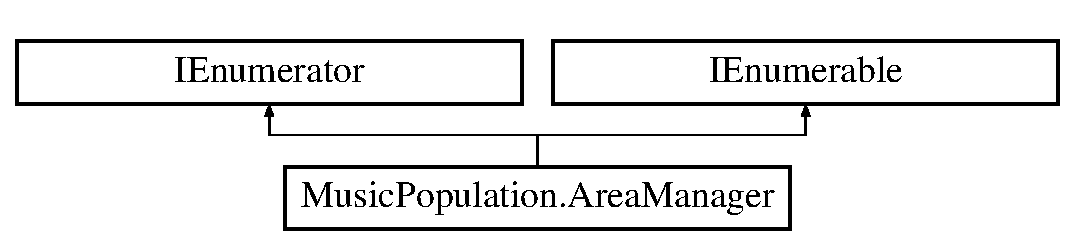
\includegraphics[height=2.000000cm]{class_music_population_1_1_area_manager}
\end{center}
\end{figure}
\subsection*{Public Member Functions}
\begin{DoxyCompactItemize}
\item 
\hyperlink{class_music_population_1_1_area_manager_ac5549e56b610d304a84e5d27dc859e29}{Area\+Manager} (int x, int y, int w, int h)
\begin{DoxyCompactList}\small\item\em Counstructs area responsible for area between (x, y) and (x+w, y+h) in static board Simulation.\+Simulation\+Board. \end{DoxyCompactList}\item 
void \hyperlink{class_music_population_1_1_area_manager_aea2e8695966595f3319c3997e051c7fc}{Kill\+Weaks\+Who\+Does\+Not\+Serve\+The\+Emperor\+Well} ()
\begin{DoxyCompactList}\small\item\em Kills the weakest individuals in area of responsibility. \end{DoxyCompactList}\item 
void \hyperlink{class_music_population_1_1_area_manager_a1cd5bdd37af092d90006e0f4899fd29d}{Select\+Champion\+Who\+Can\+Become\+Commissar} ()
\begin{DoxyCompactList}\small\item\em Selects the champion of area and copies his parameters to Champion\+Parameters property. \end{DoxyCompactList}\item 
void \hyperlink{class_music_population_1_1_area_manager_a906954fb7f6be490564d5aacc950af89}{Mutate\+Weaks\+So\+They\+Can\+Serve\+Emperor\+Better} ()
\begin{DoxyCompactList}\small\item\em Mutates each individual in area of responsibility. \end{DoxyCompactList}\item 
void \hyperlink{class_music_population_1_1_area_manager_a02826d1f1271dd9a92dc11cc43eaaf2e}{Reproduce\+Men\+To\+Have\+More\+Servants\+Of\+The\+Emperor} ()
\begin{DoxyCompactList}\small\item\em Reproduces individuals \end{DoxyCompactList}\item 
\hypertarget{class_music_population_1_1_area_manager_a56fcf125c781dd2a2435bd0f91f42fb4}{void {\bfseries Influence\+Men\+With\+Songs\+Glorifying\+Emperor} ()}\label{class_music_population_1_1_area_manager_a56fcf125c781dd2a2435bd0f91f42fb4}

\item 
\hypertarget{class_music_population_1_1_area_manager_a2429a1af1ec0f63206688874845fc314}{void {\bfseries Move\+Your\+Men\+Sergant} ()}\label{class_music_population_1_1_area_manager_a2429a1af1ec0f63206688874845fc314}

\item 
void \hyperlink{class_music_population_1_1_area_manager_ac42aef4ec8c4a3789b9e94bf40f31b04}{Regroup\+Your\+Men\+To\+Other\+Front} (int dir)
\begin{DoxyCompactList}\small\item\em Moves Individuals in given direction \end{DoxyCompactList}\item 
\hypertarget{class_music_population_1_1_area_manager_a6acfc222bc4baa96a6f3a32b9e154cc3}{I\+Enumerator {\bfseries Get\+Enumerator} ()}\label{class_music_population_1_1_area_manager_a6acfc222bc4baa96a6f3a32b9e154cc3}

\item 
\hypertarget{class_music_population_1_1_area_manager_ab91f224fd25e2ae5715496c881a2c90a}{bool {\bfseries Move\+Next} ()}\label{class_music_population_1_1_area_manager_ab91f224fd25e2ae5715496c881a2c90a}

\item 
\hypertarget{class_music_population_1_1_area_manager_a2639a5ef9ebb562d9bd1dcfd2c0f83e3}{void {\bfseries Reset} ()}\label{class_music_population_1_1_area_manager_a2639a5ef9ebb562d9bd1dcfd2c0f83e3}

\end{DoxyCompactItemize}
\subsection*{Properties}
\begin{DoxyCompactItemize}
\item 
int \hyperlink{class_music_population_1_1_area_manager_aefd6bf2d6e3330f4648b2e4f1f43bec9}{Population\+Growth}\hspace{0.3cm}{\ttfamily  \mbox{[}get\mbox{]}}
\begin{DoxyCompactList}\small\item\em Property which counts Population Growth in area of responsibility. \end{DoxyCompactList}\item 
Tuple$<$ int, int\mbox{[},\mbox{]}$>$ \hyperlink{class_music_population_1_1_area_manager_a86c18c633b2331918caed26574120933}{Champion\+Parameters}\hspace{0.3cm}{\ttfamily  \mbox{[}get\mbox{]}}
\begin{DoxyCompactList}\small\item\em Property which saves parameters of champion in area of object's responsibility. Item1 is number of notes Item2 is array of notes \end{DoxyCompactList}\item 
\hypertarget{class_music_population_1_1_area_manager_ab12ffa91c850c5a510f248e87c2cfd63}{object {\bfseries Current}\hspace{0.3cm}{\ttfamily  \mbox{[}get\mbox{]}}}\label{class_music_population_1_1_area_manager_ab12ffa91c850c5a510f248e87c2cfd63}

\end{DoxyCompactItemize}


\subsection{Detailed Description}
Class responsible for area management. It implements evolutionary algorithms which 



\subsection{Constructor \& Destructor Documentation}
\hypertarget{class_music_population_1_1_area_manager_ac5549e56b610d304a84e5d27dc859e29}{\index{Music\+Population\+::\+Area\+Manager@{Music\+Population\+::\+Area\+Manager}!Area\+Manager@{Area\+Manager}}
\index{Area\+Manager@{Area\+Manager}!Music\+Population\+::\+Area\+Manager@{Music\+Population\+::\+Area\+Manager}}
\subsubsection[{Area\+Manager}]{\setlength{\rightskip}{0pt plus 5cm}Music\+Population.\+Area\+Manager.\+Area\+Manager (
\begin{DoxyParamCaption}
\item[{int}]{x, }
\item[{int}]{y, }
\item[{int}]{w, }
\item[{int}]{h}
\end{DoxyParamCaption}
)}}\label{class_music_population_1_1_area_manager_ac5549e56b610d304a84e5d27dc859e29}


Counstructs area responsible for area between (x, y) and (x+w, y+h) in static board Simulation.\+Simulation\+Board. 



\subsection{Member Function Documentation}
\hypertarget{class_music_population_1_1_area_manager_aea2e8695966595f3319c3997e051c7fc}{\index{Music\+Population\+::\+Area\+Manager@{Music\+Population\+::\+Area\+Manager}!Kill\+Weaks\+Who\+Does\+Not\+Serve\+The\+Emperor\+Well@{Kill\+Weaks\+Who\+Does\+Not\+Serve\+The\+Emperor\+Well}}
\index{Kill\+Weaks\+Who\+Does\+Not\+Serve\+The\+Emperor\+Well@{Kill\+Weaks\+Who\+Does\+Not\+Serve\+The\+Emperor\+Well}!Music\+Population\+::\+Area\+Manager@{Music\+Population\+::\+Area\+Manager}}
\subsubsection[{Kill\+Weaks\+Who\+Does\+Not\+Serve\+The\+Emperor\+Well}]{\setlength{\rightskip}{0pt plus 5cm}void Music\+Population.\+Area\+Manager.\+Kill\+Weaks\+Who\+Does\+Not\+Serve\+The\+Emperor\+Well (
\begin{DoxyParamCaption}
{}
\end{DoxyParamCaption}
)}}\label{class_music_population_1_1_area_manager_aea2e8695966595f3319c3997e051c7fc}


Kills the weakest individuals in area of responsibility. 

\hypertarget{class_music_population_1_1_area_manager_a906954fb7f6be490564d5aacc950af89}{\index{Music\+Population\+::\+Area\+Manager@{Music\+Population\+::\+Area\+Manager}!Mutate\+Weaks\+So\+They\+Can\+Serve\+Emperor\+Better@{Mutate\+Weaks\+So\+They\+Can\+Serve\+Emperor\+Better}}
\index{Mutate\+Weaks\+So\+They\+Can\+Serve\+Emperor\+Better@{Mutate\+Weaks\+So\+They\+Can\+Serve\+Emperor\+Better}!Music\+Population\+::\+Area\+Manager@{Music\+Population\+::\+Area\+Manager}}
\subsubsection[{Mutate\+Weaks\+So\+They\+Can\+Serve\+Emperor\+Better}]{\setlength{\rightskip}{0pt plus 5cm}void Music\+Population.\+Area\+Manager.\+Mutate\+Weaks\+So\+They\+Can\+Serve\+Emperor\+Better (
\begin{DoxyParamCaption}
{}
\end{DoxyParamCaption}
)}}\label{class_music_population_1_1_area_manager_a906954fb7f6be490564d5aacc950af89}


Mutates each individual in area of responsibility. 

\hypertarget{class_music_population_1_1_area_manager_ac42aef4ec8c4a3789b9e94bf40f31b04}{\index{Music\+Population\+::\+Area\+Manager@{Music\+Population\+::\+Area\+Manager}!Regroup\+Your\+Men\+To\+Other\+Front@{Regroup\+Your\+Men\+To\+Other\+Front}}
\index{Regroup\+Your\+Men\+To\+Other\+Front@{Regroup\+Your\+Men\+To\+Other\+Front}!Music\+Population\+::\+Area\+Manager@{Music\+Population\+::\+Area\+Manager}}
\subsubsection[{Regroup\+Your\+Men\+To\+Other\+Front}]{\setlength{\rightskip}{0pt plus 5cm}void Music\+Population.\+Area\+Manager.\+Regroup\+Your\+Men\+To\+Other\+Front (
\begin{DoxyParamCaption}
\item[{int}]{dir}
\end{DoxyParamCaption}
)}}\label{class_music_population_1_1_area_manager_ac42aef4ec8c4a3789b9e94bf40f31b04}


Moves Individuals in given direction 


\begin{DoxyParams}{Parameters}
{\em dir} & 0 -\/ north, 1 -\/ south, 2 -\/ west, 3 -\/ east\\
\hline
\end{DoxyParams}
\hypertarget{class_music_population_1_1_area_manager_a02826d1f1271dd9a92dc11cc43eaaf2e}{\index{Music\+Population\+::\+Area\+Manager@{Music\+Population\+::\+Area\+Manager}!Reproduce\+Men\+To\+Have\+More\+Servants\+Of\+The\+Emperor@{Reproduce\+Men\+To\+Have\+More\+Servants\+Of\+The\+Emperor}}
\index{Reproduce\+Men\+To\+Have\+More\+Servants\+Of\+The\+Emperor@{Reproduce\+Men\+To\+Have\+More\+Servants\+Of\+The\+Emperor}!Music\+Population\+::\+Area\+Manager@{Music\+Population\+::\+Area\+Manager}}
\subsubsection[{Reproduce\+Men\+To\+Have\+More\+Servants\+Of\+The\+Emperor}]{\setlength{\rightskip}{0pt plus 5cm}void Music\+Population.\+Area\+Manager.\+Reproduce\+Men\+To\+Have\+More\+Servants\+Of\+The\+Emperor (
\begin{DoxyParamCaption}
{}
\end{DoxyParamCaption}
)}}\label{class_music_population_1_1_area_manager_a02826d1f1271dd9a92dc11cc43eaaf2e}


Reproduces individuals 

\hypertarget{class_music_population_1_1_area_manager_a1cd5bdd37af092d90006e0f4899fd29d}{\index{Music\+Population\+::\+Area\+Manager@{Music\+Population\+::\+Area\+Manager}!Select\+Champion\+Who\+Can\+Become\+Commissar@{Select\+Champion\+Who\+Can\+Become\+Commissar}}
\index{Select\+Champion\+Who\+Can\+Become\+Commissar@{Select\+Champion\+Who\+Can\+Become\+Commissar}!Music\+Population\+::\+Area\+Manager@{Music\+Population\+::\+Area\+Manager}}
\subsubsection[{Select\+Champion\+Who\+Can\+Become\+Commissar}]{\setlength{\rightskip}{0pt plus 5cm}void Music\+Population.\+Area\+Manager.\+Select\+Champion\+Who\+Can\+Become\+Commissar (
\begin{DoxyParamCaption}
{}
\end{DoxyParamCaption}
)}}\label{class_music_population_1_1_area_manager_a1cd5bdd37af092d90006e0f4899fd29d}


Selects the champion of area and copies his parameters to Champion\+Parameters property. 



\subsection{Property Documentation}
\hypertarget{class_music_population_1_1_area_manager_a86c18c633b2331918caed26574120933}{\index{Music\+Population\+::\+Area\+Manager@{Music\+Population\+::\+Area\+Manager}!Champion\+Parameters@{Champion\+Parameters}}
\index{Champion\+Parameters@{Champion\+Parameters}!Music\+Population\+::\+Area\+Manager@{Music\+Population\+::\+Area\+Manager}}
\subsubsection[{Champion\+Parameters}]{\setlength{\rightskip}{0pt plus 5cm}Tuple$<$int, int\mbox{[},\mbox{]}$>$ Music\+Population.\+Area\+Manager.\+Champion\+Parameters\hspace{0.3cm}{\ttfamily [get]}}}\label{class_music_population_1_1_area_manager_a86c18c633b2331918caed26574120933}


Property which saves parameters of champion in area of object's responsibility. Item1 is number of notes Item2 is array of notes 

\hypertarget{class_music_population_1_1_area_manager_aefd6bf2d6e3330f4648b2e4f1f43bec9}{\index{Music\+Population\+::\+Area\+Manager@{Music\+Population\+::\+Area\+Manager}!Population\+Growth@{Population\+Growth}}
\index{Population\+Growth@{Population\+Growth}!Music\+Population\+::\+Area\+Manager@{Music\+Population\+::\+Area\+Manager}}
\subsubsection[{Population\+Growth}]{\setlength{\rightskip}{0pt plus 5cm}int Music\+Population.\+Area\+Manager.\+Population\+Growth\hspace{0.3cm}{\ttfamily [get]}}}\label{class_music_population_1_1_area_manager_aefd6bf2d6e3330f4648b2e4f1f43bec9}


Property which counts Population Growth in area of responsibility. 



The documentation for this class was generated from the following file\+:\begin{DoxyCompactItemize}
\item 
C\+:/\+Users/praktykant/\+Documents/\+Git\+Hub/\+Harmony-\/\+Simulation/\+Populo/\+Music\+Population/\+Components/\+Area/Area\+Manager.\+cs\end{DoxyCompactItemize}

\hypertarget{class_music_population_1_1_area_thread}{\section{Music\+Population.\+Area\+Thread Class Reference}
\label{class_music_population_1_1_area_thread}\index{Music\+Population.\+Area\+Thread@{Music\+Population.\+Area\+Thread}}
}


Class responsible for area thread management  


\subsection*{Public Member Functions}
\begin{DoxyCompactItemize}
\item 
\hyperlink{class_music_population_1_1_area_thread_a83764cb07a09bfada3656fd3377d0aae}{Area\+Thread} (int index)
\begin{DoxyCompactList}\small\item\em Constructs new object responsible for given area. \end{DoxyCompactList}\item 
void \hyperlink{class_music_population_1_1_area_thread_a9098b4cc52c26764a28d58ceee033902}{Evolve\+Part1} ()
\begin{DoxyCompactList}\small\item\em First part of evolution. \end{DoxyCompactList}\item 
void \hyperlink{class_music_population_1_1_area_thread_ab0eb9479b65271d4e8647cbea10a3a90}{Evolve\+Part2} ()
\begin{DoxyCompactList}\small\item\em Second part of evolution. \end{DoxyCompactList}\item 
void \hyperlink{class_music_population_1_1_area_thread_ae24a83aeabfb8a254321c80097c0c17b}{Evolve\+Part3} ()
\begin{DoxyCompactList}\small\item\em Third part of evolution. \end{DoxyCompactList}\item 
void \hyperlink{class_music_population_1_1_area_thread_aa40d3faeccd473c84d31976b00ff3ec8}{Evolve\+Part4} ()
\begin{DoxyCompactList}\small\item\em Fourth part of evolution. \end{DoxyCompactList}\item 
void \hyperlink{class_music_population_1_1_area_thread_aa055713a70d3f4d4a22bfb482c8f884c}{Evolve\+Part5} ()
\begin{DoxyCompactList}\small\item\em Fifth part of evolution. \end{DoxyCompactList}\end{DoxyCompactItemize}


\subsection{Detailed Description}
Class responsible for area thread management 



\subsection{Constructor \& Destructor Documentation}
\hypertarget{class_music_population_1_1_area_thread_a83764cb07a09bfada3656fd3377d0aae}{\index{Music\+Population\+::\+Area\+Thread@{Music\+Population\+::\+Area\+Thread}!Area\+Thread@{Area\+Thread}}
\index{Area\+Thread@{Area\+Thread}!Music\+Population\+::\+Area\+Thread@{Music\+Population\+::\+Area\+Thread}}
\subsubsection[{Area\+Thread}]{\setlength{\rightskip}{0pt plus 5cm}Music\+Population.\+Area\+Thread.\+Area\+Thread (
\begin{DoxyParamCaption}
\item[{int}]{index}
\end{DoxyParamCaption}
)}}\label{class_music_population_1_1_area_thread_a83764cb07a09bfada3656fd3377d0aae}


Constructs new object responsible for given area. 


\begin{DoxyParams}{Parameters}
{\em index} & Number of area, integer between 0 and 15.\\
\hline
\end{DoxyParams}


\subsection{Member Function Documentation}
\hypertarget{class_music_population_1_1_area_thread_a9098b4cc52c26764a28d58ceee033902}{\index{Music\+Population\+::\+Area\+Thread@{Music\+Population\+::\+Area\+Thread}!Evolve\+Part1@{Evolve\+Part1}}
\index{Evolve\+Part1@{Evolve\+Part1}!Music\+Population\+::\+Area\+Thread@{Music\+Population\+::\+Area\+Thread}}
\subsubsection[{Evolve\+Part1}]{\setlength{\rightskip}{0pt plus 5cm}void Music\+Population.\+Area\+Thread.\+Evolve\+Part1 (
\begin{DoxyParamCaption}
{}
\end{DoxyParamCaption}
)}}\label{class_music_population_1_1_area_thread_a9098b4cc52c26764a28d58ceee033902}


First part of evolution. 

\hypertarget{class_music_population_1_1_area_thread_ab0eb9479b65271d4e8647cbea10a3a90}{\index{Music\+Population\+::\+Area\+Thread@{Music\+Population\+::\+Area\+Thread}!Evolve\+Part2@{Evolve\+Part2}}
\index{Evolve\+Part2@{Evolve\+Part2}!Music\+Population\+::\+Area\+Thread@{Music\+Population\+::\+Area\+Thread}}
\subsubsection[{Evolve\+Part2}]{\setlength{\rightskip}{0pt plus 5cm}void Music\+Population.\+Area\+Thread.\+Evolve\+Part2 (
\begin{DoxyParamCaption}
{}
\end{DoxyParamCaption}
)}}\label{class_music_population_1_1_area_thread_ab0eb9479b65271d4e8647cbea10a3a90}


Second part of evolution. 

\hypertarget{class_music_population_1_1_area_thread_ae24a83aeabfb8a254321c80097c0c17b}{\index{Music\+Population\+::\+Area\+Thread@{Music\+Population\+::\+Area\+Thread}!Evolve\+Part3@{Evolve\+Part3}}
\index{Evolve\+Part3@{Evolve\+Part3}!Music\+Population\+::\+Area\+Thread@{Music\+Population\+::\+Area\+Thread}}
\subsubsection[{Evolve\+Part3}]{\setlength{\rightskip}{0pt plus 5cm}void Music\+Population.\+Area\+Thread.\+Evolve\+Part3 (
\begin{DoxyParamCaption}
{}
\end{DoxyParamCaption}
)}}\label{class_music_population_1_1_area_thread_ae24a83aeabfb8a254321c80097c0c17b}


Third part of evolution. 

\hypertarget{class_music_population_1_1_area_thread_aa40d3faeccd473c84d31976b00ff3ec8}{\index{Music\+Population\+::\+Area\+Thread@{Music\+Population\+::\+Area\+Thread}!Evolve\+Part4@{Evolve\+Part4}}
\index{Evolve\+Part4@{Evolve\+Part4}!Music\+Population\+::\+Area\+Thread@{Music\+Population\+::\+Area\+Thread}}
\subsubsection[{Evolve\+Part4}]{\setlength{\rightskip}{0pt plus 5cm}void Music\+Population.\+Area\+Thread.\+Evolve\+Part4 (
\begin{DoxyParamCaption}
{}
\end{DoxyParamCaption}
)}}\label{class_music_population_1_1_area_thread_aa40d3faeccd473c84d31976b00ff3ec8}


Fourth part of evolution. 

\hypertarget{class_music_population_1_1_area_thread_aa055713a70d3f4d4a22bfb482c8f884c}{\index{Music\+Population\+::\+Area\+Thread@{Music\+Population\+::\+Area\+Thread}!Evolve\+Part5@{Evolve\+Part5}}
\index{Evolve\+Part5@{Evolve\+Part5}!Music\+Population\+::\+Area\+Thread@{Music\+Population\+::\+Area\+Thread}}
\subsubsection[{Evolve\+Part5}]{\setlength{\rightskip}{0pt plus 5cm}void Music\+Population.\+Area\+Thread.\+Evolve\+Part5 (
\begin{DoxyParamCaption}
{}
\end{DoxyParamCaption}
)}}\label{class_music_population_1_1_area_thread_aa055713a70d3f4d4a22bfb482c8f884c}


Fifth part of evolution. 



The documentation for this class was generated from the following file\+:\begin{DoxyCompactItemize}
\item 
C\+:/\+Users/praktykant/\+Documents/\+Git\+Hub/\+Harmony-\/\+Simulation/\+Populo/\+Music\+Population/\+Components/\+Area/Area\+Thread.\+cs\end{DoxyCompactItemize}

\hypertarget{class_music_population_1_1_board}{\section{Music\+Population.\+Board Class Reference}
\label{class_music_population_1_1_board}\index{Music\+Population.\+Board@{Music\+Population.\+Board}}
}


Represents simulation board.  


\subsection*{Public Member Functions}
\begin{DoxyCompactItemize}
\item 
\hyperlink{class_music_population_1_1_board_af3767b8609c26674c30bf536db221db3}{Board} ()
\begin{DoxyCompactList}\small\item\em Constructs new \hyperlink{class_music_population_1_1_board}{Board} filled with random values and in first phase. \end{DoxyCompactList}\item 
void \hyperlink{class_music_population_1_1_board_aa3525b70d6179fc9b9377431e7a09303}{Change\+Phase} ()
\begin{DoxyCompactList}\small\item\em Method responsible for changing simulation phase. \end{DoxyCompactList}\item 
bool \hyperlink{class_music_population_1_1_board_a2d2aed951c7749bab64d447979e11db2}{Is\+Legal} (int x, int y)
\begin{DoxyCompactList}\small\item\em Returns whether point (x, y) is legal or not. \end{DoxyCompactList}\item 
Tuple$<$ int, int $>$ \hyperlink{class_music_population_1_1_board_aace7e7443efbe0e3b1298dd553c7b8e8}{Get\+Best\+In\+Area} (int x1, int y1, int x2, int y2)
\begin{DoxyCompactList}\small\item\em Returns best individual in rectangle determined by positions (x1, y1), (x2, y2) \end{DoxyCompactList}\item 
void \hyperlink{class_music_population_1_1_board_a1e1ececc516d74bbdcf254fd61075253}{Move\+Individual} (int s\+X, int s\+Y, int d\+X, int d\+Y)
\begin{DoxyCompactList}\small\item\em Moves individual in (s\+X, s\+Y) to (d\+X, d\+Y). \end{DoxyCompactList}\item 
void \hyperlink{class_music_population_1_1_board_aad68697f57bb84e480c448e85eb0128e}{Copy\+Individual} (int s\+X, int s\+Y, int d\+X, int d\+Y)
\begin{DoxyCompactList}\small\item\em Copies individual in (s\+X,s\+Y) to (d\+X, d\+Y). \end{DoxyCompactList}\end{DoxyCompactItemize}
\subsection*{Public Attributes}
\begin{DoxyCompactItemize}
\item 
\hypertarget{class_music_population_1_1_board_ac394649f4b46b9df6162738673548e5f}{const int {\bfseries Board\+Width} = 256}\label{class_music_population_1_1_board_ac394649f4b46b9df6162738673548e5f}

\item 
\hypertarget{class_music_population_1_1_board_a703b732a7e262d7e973ce12f4d0bb53c}{const int {\bfseries Init\+Population\+Growth} = 256 $\ast$ 256 / 2}\label{class_music_population_1_1_board_a703b732a7e262d7e973ce12f4d0bb53c}

\end{DoxyCompactItemize}
\subsection*{Properties}
\begin{DoxyCompactItemize}
\item 
\hyperlink{class_music_population_1_1_member}{Member} \hyperlink{class_music_population_1_1_board_abd14bb128680a5f37fc29f006e65e4f0}{this\mbox{[}int i, int j\mbox{]}}\hspace{0.3cm}{\ttfamily  \mbox{[}get, set\mbox{]}}
\begin{DoxyCompactList}\small\item\em Basic board getter, if index is out of range returns null. \end{DoxyCompactList}\item 
int \hyperlink{class_music_population_1_1_board_abaf64b14d42081829501c6958e2199aa}{Index\+Of\+Phase}\hspace{0.3cm}{\ttfamily  \mbox{[}get\mbox{]}}
\begin{DoxyCompactList}\small\item\em Getter which returns index of phase. \end{DoxyCompactList}\item 
string \hyperlink{class_music_population_1_1_board_af0fe9cecfaf3577bf9ea697c4e909e96}{Rank\+Table\+Msg}\hspace{0.3cm}{\ttfamily  \mbox{[}get\mbox{]}}
\begin{DoxyCompactList}\small\item\em Retrurns string representing all ranks in board. \end{DoxyCompactList}\item 
int \hyperlink{class_music_population_1_1_board_aedfe71556d1fe32c58a134a868e827c1}{Population\+Growth}\hspace{0.3cm}{\ttfamily  \mbox{[}get\mbox{]}}
\begin{DoxyCompactList}\small\item\em Returns Population Growth in board. \end{DoxyCompactList}\end{DoxyCompactItemize}


\subsection{Detailed Description}
Represents simulation board. 

Global Parameters used in board. 

\subsection{Constructor \& Destructor Documentation}
\hypertarget{class_music_population_1_1_board_af3767b8609c26674c30bf536db221db3}{\index{Music\+Population\+::\+Board@{Music\+Population\+::\+Board}!Board@{Board}}
\index{Board@{Board}!Music\+Population\+::\+Board@{Music\+Population\+::\+Board}}
\subsubsection[{Board}]{\setlength{\rightskip}{0pt plus 5cm}Music\+Population.\+Board.\+Board (
\begin{DoxyParamCaption}
{}
\end{DoxyParamCaption}
)}}\label{class_music_population_1_1_board_af3767b8609c26674c30bf536db221db3}


Constructs new \hyperlink{class_music_population_1_1_board}{Board} filled with random values and in first phase. 



\subsection{Member Function Documentation}
\hypertarget{class_music_population_1_1_board_aa3525b70d6179fc9b9377431e7a09303}{\index{Music\+Population\+::\+Board@{Music\+Population\+::\+Board}!Change\+Phase@{Change\+Phase}}
\index{Change\+Phase@{Change\+Phase}!Music\+Population\+::\+Board@{Music\+Population\+::\+Board}}
\subsubsection[{Change\+Phase}]{\setlength{\rightskip}{0pt plus 5cm}void Music\+Population.\+Board.\+Change\+Phase (
\begin{DoxyParamCaption}
{}
\end{DoxyParamCaption}
)}}\label{class_music_population_1_1_board_aa3525b70d6179fc9b9377431e7a09303}


Method responsible for changing simulation phase. 

\hypertarget{class_music_population_1_1_board_aad68697f57bb84e480c448e85eb0128e}{\index{Music\+Population\+::\+Board@{Music\+Population\+::\+Board}!Copy\+Individual@{Copy\+Individual}}
\index{Copy\+Individual@{Copy\+Individual}!Music\+Population\+::\+Board@{Music\+Population\+::\+Board}}
\subsubsection[{Copy\+Individual}]{\setlength{\rightskip}{0pt plus 5cm}void Music\+Population.\+Board.\+Copy\+Individual (
\begin{DoxyParamCaption}
\item[{int}]{s\+X, }
\item[{int}]{s\+Y, }
\item[{int}]{d\+X, }
\item[{int}]{d\+Y}
\end{DoxyParamCaption}
)}}\label{class_music_population_1_1_board_aad68697f57bb84e480c448e85eb0128e}


Copies individual in (s\+X,s\+Y) to (d\+X, d\+Y). 

\hypertarget{class_music_population_1_1_board_aace7e7443efbe0e3b1298dd553c7b8e8}{\index{Music\+Population\+::\+Board@{Music\+Population\+::\+Board}!Get\+Best\+In\+Area@{Get\+Best\+In\+Area}}
\index{Get\+Best\+In\+Area@{Get\+Best\+In\+Area}!Music\+Population\+::\+Board@{Music\+Population\+::\+Board}}
\subsubsection[{Get\+Best\+In\+Area}]{\setlength{\rightskip}{0pt plus 5cm}Tuple$<$int, int$>$ Music\+Population.\+Board.\+Get\+Best\+In\+Area (
\begin{DoxyParamCaption}
\item[{int}]{x1, }
\item[{int}]{y1, }
\item[{int}]{x2, }
\item[{int}]{y2}
\end{DoxyParamCaption}
)}}\label{class_music_population_1_1_board_aace7e7443efbe0e3b1298dd553c7b8e8}


Returns best individual in rectangle determined by positions (x1, y1), (x2, y2) 

\hypertarget{class_music_population_1_1_board_a2d2aed951c7749bab64d447979e11db2}{\index{Music\+Population\+::\+Board@{Music\+Population\+::\+Board}!Is\+Legal@{Is\+Legal}}
\index{Is\+Legal@{Is\+Legal}!Music\+Population\+::\+Board@{Music\+Population\+::\+Board}}
\subsubsection[{Is\+Legal}]{\setlength{\rightskip}{0pt plus 5cm}bool Music\+Population.\+Board.\+Is\+Legal (
\begin{DoxyParamCaption}
\item[{int}]{x, }
\item[{int}]{y}
\end{DoxyParamCaption}
)}}\label{class_music_population_1_1_board_a2d2aed951c7749bab64d447979e11db2}


Returns whether point (x, y) is legal or not. 

\hypertarget{class_music_population_1_1_board_a1e1ececc516d74bbdcf254fd61075253}{\index{Music\+Population\+::\+Board@{Music\+Population\+::\+Board}!Move\+Individual@{Move\+Individual}}
\index{Move\+Individual@{Move\+Individual}!Music\+Population\+::\+Board@{Music\+Population\+::\+Board}}
\subsubsection[{Move\+Individual}]{\setlength{\rightskip}{0pt plus 5cm}void Music\+Population.\+Board.\+Move\+Individual (
\begin{DoxyParamCaption}
\item[{int}]{s\+X, }
\item[{int}]{s\+Y, }
\item[{int}]{d\+X, }
\item[{int}]{d\+Y}
\end{DoxyParamCaption}
)}}\label{class_music_population_1_1_board_a1e1ececc516d74bbdcf254fd61075253}


Moves individual in (s\+X, s\+Y) to (d\+X, d\+Y). 



\subsection{Property Documentation}
\hypertarget{class_music_population_1_1_board_abaf64b14d42081829501c6958e2199aa}{\index{Music\+Population\+::\+Board@{Music\+Population\+::\+Board}!Index\+Of\+Phase@{Index\+Of\+Phase}}
\index{Index\+Of\+Phase@{Index\+Of\+Phase}!Music\+Population\+::\+Board@{Music\+Population\+::\+Board}}
\subsubsection[{Index\+Of\+Phase}]{\setlength{\rightskip}{0pt plus 5cm}int Music\+Population.\+Board.\+Index\+Of\+Phase\hspace{0.3cm}{\ttfamily [get]}}}\label{class_music_population_1_1_board_abaf64b14d42081829501c6958e2199aa}


Getter which returns index of phase. 

\hypertarget{class_music_population_1_1_board_aedfe71556d1fe32c58a134a868e827c1}{\index{Music\+Population\+::\+Board@{Music\+Population\+::\+Board}!Population\+Growth@{Population\+Growth}}
\index{Population\+Growth@{Population\+Growth}!Music\+Population\+::\+Board@{Music\+Population\+::\+Board}}
\subsubsection[{Population\+Growth}]{\setlength{\rightskip}{0pt plus 5cm}int Music\+Population.\+Board.\+Population\+Growth\hspace{0.3cm}{\ttfamily [get]}}}\label{class_music_population_1_1_board_aedfe71556d1fe32c58a134a868e827c1}


Returns Population Growth in board. 

\hypertarget{class_music_population_1_1_board_af0fe9cecfaf3577bf9ea697c4e909e96}{\index{Music\+Population\+::\+Board@{Music\+Population\+::\+Board}!Rank\+Table\+Msg@{Rank\+Table\+Msg}}
\index{Rank\+Table\+Msg@{Rank\+Table\+Msg}!Music\+Population\+::\+Board@{Music\+Population\+::\+Board}}
\subsubsection[{Rank\+Table\+Msg}]{\setlength{\rightskip}{0pt plus 5cm}string Music\+Population.\+Board.\+Rank\+Table\+Msg\hspace{0.3cm}{\ttfamily [get]}}}\label{class_music_population_1_1_board_af0fe9cecfaf3577bf9ea697c4e909e96}


Retrurns string representing all ranks in board. 

\hypertarget{class_music_population_1_1_board_abd14bb128680a5f37fc29f006e65e4f0}{\index{Music\+Population\+::\+Board@{Music\+Population\+::\+Board}!this\mbox{[}int i, int j\mbox{]}@{this[int i, int j]}}
\index{this\mbox{[}int i, int j\mbox{]}@{this[int i, int j]}!Music\+Population\+::\+Board@{Music\+Population\+::\+Board}}
\subsubsection[{this[int i, int j]}]{\setlength{\rightskip}{0pt plus 5cm}{\bf Member} Music\+Population.\+Board.\+this\mbox{[}int i, int j\mbox{]}\hspace{0.3cm}{\ttfamily [get]}, {\ttfamily [set]}}}\label{class_music_population_1_1_board_abd14bb128680a5f37fc29f006e65e4f0}


Basic board getter, if index is out of range returns null. 



The documentation for this class was generated from the following files\+:\begin{DoxyCompactItemize}
\item 
C\+:/\+Users/praktykant/\+Documents/\+Git\+Hub/\+Harmony-\/\+Simulation/\+Populo/\+Music\+Population/\+Components/\+Board/Board.\+cs\item 
C\+:/\+Users/praktykant/\+Documents/\+Git\+Hub/\+Harmony-\/\+Simulation/\+Populo/\+Music\+Population/\+Components/\+Board/Board\+Parameters.\+cs\end{DoxyCompactItemize}

\hypertarget{class_periodic_chords_1_1_chord}{\section{Periodic\+Chords.\+Chord Class Reference}
\label{class_periodic_chords_1_1_chord}\index{Periodic\+Chords.\+Chord@{Periodic\+Chords.\+Chord}}
}
Inheritance diagram for Periodic\+Chords.\+Chord\+:\begin{figure}[H]
\begin{center}
\leavevmode
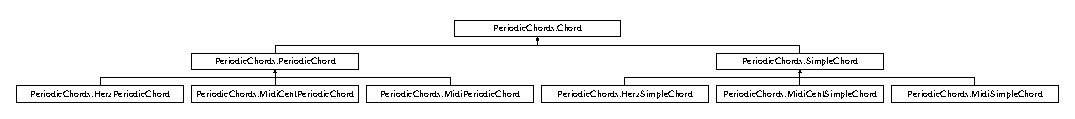
\includegraphics[height=1.147541cm]{class_periodic_chords_1_1_chord}
\end{center}
\end{figure}
\subsection*{Public Member Functions}
\begin{DoxyCompactItemize}
\item 
\hypertarget{class_periodic_chords_1_1_chord_a833cdd245bc463ddb56e162617fd6a5b}{double {\bfseries Note\+To\+Frequency} (double note)}\label{class_periodic_chords_1_1_chord_a833cdd245bc463ddb56e162617fd6a5b}

\item 
\hypertarget{class_periodic_chords_1_1_chord_a3799e69892f39fbcff97d5033febb188}{double {\bfseries Frequency\+To\+Note} (double frequency)}\label{class_periodic_chords_1_1_chord_a3799e69892f39fbcff97d5033febb188}

\end{DoxyCompactItemize}
\subsection*{Public Attributes}
\begin{DoxyCompactItemize}
\item 
\hypertarget{class_periodic_chords_1_1_chord_ae60e1f9c163dc891516e927dd0708e78}{readonly double\mbox{[}$\,$\mbox{]} {\bfseries n2f} = \{8.\+175798915643707, 8.\+18052280646487, 8.\+185249426700578, 8.\+18997877792786, 8.\+19471086172465, 8.\+199445679669807, 8.\+204183233343088, 8.\+208923524325167, 8.\+213666554197633, 8.\+218412324542992, 8.\+223160836944654, 8.\+227912092986948, 8.\+232666094255134, 8.\+237422842335365, 8.\+242182338814722, 8.\+246944585281202, 8.\+251709583323718, 8.\+256477334532102, 8.\+261247840497097, 8.\+266021102810386, 8.\+270797123064552, 8.\+275575902853102, 8.\+280357443770471, 8.\+285141747412005, 8.\+289928815373974, 8.\+294718649253586, 8.\+29951125064895, 8.\+30430662115911, 8.\+309104762384031, 8.\+313905675924602, 8.\+318709363382638, 8.\+323515826360877, 8.\+328325066462991, 8.\+333137085293572, 8.\+337951884458139, 8.\+342769465563139, 8.\+347589830215949, 8.\+352412980024873, 8.\+357238916599139, 8.\+362067641548922, 8.\+366899156485312, 8.\+371733463020334, 8.\+376570562766942, 8.\+381410457339024, 8.\+386253148351406, 8.\+391098637419832, 8.\+395946926160999, 8.\+400798016192526, 8.\+405651909132972, 8.\+410508606601821, 8.\+415368110219507, 8.\+420230421607389, 8.\+425095542387762, 8.\+429963474183877, 8.\+434834218619903, 8.\+439707777320951, 8.\+444584151913078, 8.\+449463344023274, 8.\+454345355279466, 8.\+459230187310538, 8.\+464117841746297, 8.\+469008320217505, 8.\+473901624355852, 8.\+478797755793984, 8.\+483696716165483, 8.\+488598507104873, 8.\+493503130247635, 8.\+498410587230184, 8.\+503320879689882, 8.\+508234009265037, 8.\+513149977594903, 8.\+518068786319686, 8.\+52299043708053, 8.\+527914931519545, 8.\+532842271279769, 8.\+537772458005202, 8.\+542705493340792, 8.\+547641378932434, 8.\+552580116426977, 8.\+557521707472214, 8.\+562466153716906, 8.\+567413456810757, 8.\+572363618404419, 8.\+577316640149506, 8.\+582272523698583, 8.\+587231270705171, 8.\+59219288282374, 8.\+597157361709732, 8.\+60212470901953, 8.\+607094926410479, 8.\+612068015540881, 8.\+617043978069997, 8.\+622022815658049, 8.\+627004529966209, 8.\+631989122656625, 8.\+636976595392392, 8.\+64196694983757, 8.\+646960187657182, 8.\+651956310517207, 8.\+656955320084592, 8.\+661957218027252, 8.\+666962006014055, 8.\+67196968571484, 8.\+676980258800409, 8.\+681993726942528, 8.\+687010091813933, 8.\+692029355088314, 8.\+697051518440352, 8.\+702076583545674, 8.\+707104552080883, 8.\+712135425723552, 8.\+717169206152223, 8.\+722205895046402, 8.\+727245494086565, 8.\+732288004954176, 8.\+737333429331654, 8.\+742381768902396, 8.\+747433025350764, 8.\+752487200362104, 8.\+75754429562273, 8.\+762604312819924, 8.\+767667253641966, 8.\+772733119778085, 8.\+7778019129185, 8.\+782873634754402, 8.\+787948286977961, 8.\+793025871282325, 8.\+798106389361614, 8.\+80318984291094, 8.\+808276233626385, 8.\+813365563205013, 8.\+818457833344864, 8.\+82355304574497, 8.\+828651202105325, 8.\+833752304126936, 8.\+838856353511765, 8.\+84396335196277, 8.\+849073301183893, 8.\+85418620288005, 8.\+859302058757159, 8.\+864420870522105, 8.\+869542639882779, 8.\+874667368548044, 8.\+879795058227756, 8.\+884925710632759, 8.\+890059327474884, 8.\+89519591046695, 8.\+900335461322761, 8.\+905477981757134, 8.\+910623473485849, 8.\+915771938225692, 8.\+920923377694436, 8.\+926077793610848, 8.\+93123518769469, 8.\+936395561666709, 8.\+941558917248663, 8.\+946725256163292, 8.\+951894580134333, 8.\+957066890886523, 8.\+962242190145586, 8.\+967420479638257, 8.\+972601761092251, 8.\+977786036236308, 8.\+98297330680014, 8.\+988163574514473, 8.\+993356841111027, 8.\+998553108322525, 9.\+003752377882693, 9.\+008954651526246, 9.\+014159930988926, 9.\+019368218007461, 9.\+02457951431958, 9.\+029793821664025, 9.\+035011141780537, 9.\+04023147640986, 9.\+045454827293756, 9.\+050681196174985, 9.\+055910584797308, 9.\+061142994905504, 9.\+066378428245354, 9.\+071616886563652, 9.\+07685837160819, 9.\+082102885127789, 9.\+087350428872268, 9.\+092601004592458, 9.\+097854614040202, 9.\+103111258968358, 9.\+108370941130792, 9.\+11363366228238, 9.\+118899424179034, 9.\+124168228577654, 9.\+12944007723617, 9.\+134714971913517, 9.\+13999291436966, 9.\+145273906365569, 9.\+150557949663233, 9.\+155845046025672, 9.\+161135197216907, 9.\+16642840500199, 9.\+17172467114699, 9.\+177023997418988, 9.\+1823263855861, 9.\+187631837417449, 9.\+192940354683198, 9.\+19825193915452, 9.\+203566592603613, 9.\+208884316803697, 9.\+214205113529026, 9.\+219528984554863, 9.\+224855931657517, 9.\+23018595661431, 9.\+235519061203593, 9.\+240855247204744, 9.\+246194516398173, 9.\+251536870565312, 9.\+256882311488626, 9.\+262230840951618, 9.\+26758246073881, 9.\+272937172635757, 9.\+27829497842905, 9.\+283655879906307, 9.\+289019878856186, 9.\+294386977068363, 9.\+299757176333573, 9.\+305130478443568, 9.\+310506885191137, 9.\+315886398370107, 9.\+321269019775345, 9.\+326654751202746, 9.\+332043594449248, 9.\+337435551312833, 9.\+342830623592516, 9.\+348228813088346, 9.\+353630121601425, 9.\+359034550933881, 9.\+364442102888896, 9.\+369852779270682, 9.\+375266581884508, 9.\+380683512536676, 9.\+386103573034534, 9.\+39152676518647, 9.\+396953090801924, 9.\+402382551691378, 9.\+407815149666357, 9.\+413250886539442, 9.\+418689764124254, 9.\+424131784235461, 9.\+429576948688783, 9.\+43502525930099, 9.\+440476717889887, 9.\+445931326274362, 9.\+45138908627432, 9.\+456849999710737, 9.\+462314068405634, 9.\+467781294182087, 9.\+473251678864223, 9.\+47872522427722, 9.\+484201932247323, 9.\+489681804601824, 9.\+49516484316907, 9.\+500651049778462, 9.\+506140426260464, 9.\+511632974446595, 9.\+517128696169426, 9.\+522627593262605, 9.\+528129667560822, 9.\+533634920899834, 9.\+539143355116458, 9.\+544654972048567, 9.\+550169773535105, 9.\+555687761416065, 9.\+561208937532527, 9.\+566733303726611, 9.\+572260861841515, 9.\+577791613721494, 9.\+583325561211872, 9.\+58886270615904, 9.\+594403050410449, 9.\+599946595814634, 9.\+605493344221186, 9.\+611043297480759, 9.\+616596457445088, 9.\+622152825966975, 9.\+62771240490028, 9.\+63327519609996, 9.\+638841201422021, 9.\+644410422723553, 9.\+649982861862714, 9.\+655558520698733, 9.\+661137401091919, 9.\+66671950490365, 9.\+672304833996392, 9.\+677893390233676, 9.\+683485175480111, 9.\+689080191601384, 9.\+69467844046426, 9.\+700279923936586, 9.\+705884643887275, 9.\+711492602186347, 9.\+717103800704876, 9.\+722718241315029, 9.\+72833592589005, 9.\+733956856304271, 9.\+739581034433103, 9.\+745208462153034, 9.\+750839141341656, 9.\+756473073877629, 9.\+762110261640702, 9.\+76775070651171, 9.\+773394410372578, 9.\+779041375106313, 9.\+78469160259701, 9.\+790345094729867, 9.\+796001853391152, 9.\+801661880468235, 9.\+807325177849568, 9.\+812991747424702, 9.\+818661591084275, 9.\+824334710720013, 9.\+830011108224749, 9.\+835690785492401, 9.\+841373744417977, 9.\+847059986897587, 9.\+852749514828433, 9.\+85844233010881, 9.\+864138434638125, 9.\+869837830316865, 9.\+87554051904662, 9.\+881246502730084, 9.\+886955783271045, 9.\+892668362574389, 9.\+898384242546108, 9.\+904103425093298, 9.\+909825912124154, 9.\+915551705547966, 9.\+921280807275133, 9.\+927013219217162, 9.\+93274894328666, 9.\+938487981397328, 9.\+944230335464002, 9.\+949976007402599, 9.\+95572499913015, 9.\+961477312564794, 9.\+967232949625778, 9.\+97299191223346, 9.\+9787542023093, 9.\+984519821775887, 9.\+990288772556898, 9.\+996061056577135, 10.\+001836675762508, 10.\+007615632040041, 10.\+013397927337868, 10.\+019183563585237, 10.\+024972542712524, 10.\+030764866651205, 10.\+036560537333877, 10.\+042359556694251, 10.\+048161926667161, 10.\+053967649188548, 10.\+059776726195492, 10.\+065589159626173, 10.\+071404951419899, 10.\+077224103517095, 10.\+08304661785931, 10.\+088872496389214, 10.\+09470174105059, 10.\+100534353788372, 10.\+106370336548588, 10.\+112209691278405, 10.\+118052419926109, 10.\+123898524441115, 10.\+129748006773964, 10.\+135600868876317, 10.\+141457112700984, 10.\+14731674020188, 10.\+153179753334058, 10.\+159046154053701, 10.\+164915944318121, 10.\+17078912608576, 10.\+176665701316189, 10.\+182545671970127, 10.\+188429040009408, 10.\+194315807397006, 10.\+200205976097026, 10.\+206099548074715, 10.\+211996525296447, 10.\+217896909729733, 10.\+223800703343235, 10.\+229707908106736, 10.\+235618525991162, 10.\+24153255896858, 10.\+247450009012192, 10.\+253370878096346, 10.\+25929516819652, 10.\+265222881289354, 10.\+271154019352611, 10.\+277088584365202, 10.\+283026578307185, 10.\+288968003159756, 10.\+294912860905255, 10.\+300861153527183, 10.\+30681288301017, 10.\+312768051339999, 10.\+318726660503598, 10.\+324688712489047, 10.\+33065420928557, 10.\+336623152883536, 10.\+342595545274484, 10.\+348571388451086, 10.\+354550684407169, 10.\+360533435137711, 10.\+366519642638846, 10.\+372509308907857, 10.\+378502435943181, 10.\+384499025744423, 10.\+39049908031233, 10.\+396502601648802, 10.\+402509591756907, 10.\+408520052640862, 10.\+414533986306042, 10.\+420551394758984, 10.\+426572280007393, 10.\+432596644060117, 10.\+438624488927177, 10.\+444655816619745, 10.\+450690629150166, 10.\+456728928531941, 10.\+46277071677973, 10.\+468815995909376, 10.\+474864767937866, 10.\+480917034883364, 10.\+486972798765192, 10.\+493032061603847, 10.\+499094825420979, 10.\+505161092239433, 10.\+511230864083199, 10.\+517304142977443, 10.\+523380930948502, 10.\+529461230023884, 10.\+53554504223227, 10.\+541632369603501, 10.\+547723214168618, 10.\+55381757795981, 10.\+559915463010451, 10.\+566016871355085, 10.\+572121805029438, 10.\+578230266070404, 10.\+584342256516056, 10.\+590457778405655, 10.\+596576833779633, 10.\+602699424679592, 10.\+608825553148328, 10.\+614955221229811, 10.\+621088430969188, 10.\+627225184412787, 10.\+633365483608138, 10.\+63950933060393, 10.\+645656727450048, 10.\+651807676197553, 10.\+657962178898702, 10.\+664120237606928, 10.\+670281854376851, 10.\+676447031264294, 10.\+682615770326247, 10.\+688788073620902, 10.\+69496394320763, 10.\+701143381146998, 10.\+707326389500766, 10.\+713512970331871, 10.\+719703125704468, 10.\+725896857683885, 10.\+732094168336646, 10.\+73829505973047, 10.\+744499533934274, 10.\+750707593018157, 10.\+756919239053445, 10.\+76313447411263, 10.\+769353300269412, 10.\+77557571959869, 10.\+781801734176563, 10.\+788031346080324, 10.\+79426455738847, 10.\+800501370180706, 10.\+80674178653793, 10.\+81298580854224, 10.\+819233438276944, 10.\+825484677826548, 10.\+831739529276767, 10.\+837997994714513, 10.\+844260076227924, 10.\+85052577590632, 10.\+856795095840244, 10.\+863068038121437, 10.\+869344604842855, 10.\+875624798098663, 10.\+881908619984229, 10.\+888196072596145, 10.\+894487158032202, 10.\+900781878391411, 10.\+907080235773991, 10.\+913382232281373, 10.\+91968787001621, 10.\+925997151082354, 10.\+932310077584898, 10.\+93862665163013, 10.\+944946875325565, 10.\+95127075077993, 10.\+957598280103173, 10.\+963929465406453, 10.\+970264308802175, 10.\+976602812403936, 10.\+982944978326563, 10.\+98929080868611, 10.\+99564030559985, 11.\+001993471186278, 11.\+00835030756511, 11.\+014710816857301, 11.\+021075001185018, 11.\+02744286267166, 11.\+033814403441845, 11.\+040189625621428, 11.\+046568531337488, 11.\+05295112271833, 11.\+059337401893501, 11.\+065727370993764, 11.\+072121032151124, 11.\+078518387498807, 11.\+08491943917128, 11.\+09132418930424, 11.\+097732640034613, 11.\+104144793500577, 11.\+110560651841528, 11.\+116980217198103, 11.\+12340349171218, 11.\+129830477526868, 11.\+136261176786519, 11.\+142695591636715, 11.\+149133724224297, 11.\+155575576697332, 11.\+162021151205128, 11.\+168470449898239, 11.\+174923474928459, 11.\+181380228448829, 11.\+187840712613621, 11.\+194304929578376, 11.\+200772881499864, 11.\+2072445705361, 11.\+21371999884635, 11.\+22019916859113, 11.\+22668208193219, 11.\+233168741032559, 11.\+23965914805649, 11.\+24615330516949, 11.\+252651214538325, 11.\+259152878331008, 11.\+265658298716806, 11.\+272167477866232, 11.\+278680417951072, 11.\+285197121144352, 11.\+291717589620353, 11.\+298241825554618, 11.\+304769831123943, 11.\+311301608506385, 11.\+317837159881252, 11.\+324376487429129, 11.\+330919593331842, 11.\+337466479772488, 11.\+34401714893542, 11.\+350571603006253, 11.\+35712984417187, 11.\+36369187462041, 11.\+370257696541287, 11.\+376827312125174, 11.\+383400723564009, 11.\+389977933050995, 11.\+396558942780603, 11.\+403143754948577, 11.\+409732371751916, 11.\+416324795388915, 11.\+422921028059115, 11.\+429521071963332, 11.\+436124929303661, 11.\+442732602283465, 11.\+44934409310737, 11.\+455959403981305, 11.\+462578537112446, 11.\+469201494709251, 11.\+475828278981458, 11.\+48245889214008, 11.\+489093336397406, 11.\+495731613967001, 11.\+502373727063723, 11.\+509019677903694, 11.\+51566946870432, 11.\+522323101684293, 11.\+528980579063582, 11.\+535641903063443, 11.\+5423070759064, 11.\+548976099816294, 11.\+555648977018222, 11.\+562325709738575, 11.\+569006300205032, 11.\+575690750646558, 11.\+582379063293407, 11.\+589071240377114, 11.\+59576728413052, 11.\+602467196787744, 11.\+609170980584198, 11.\+61587863775658, 11.\+622590170542892, 11.\+62930558118242, 11.\+636024871915742, 11.\+642748044984748, 11.\+649475102632602, 11.\+656206047103776, 11.\+662940880644035, 11.\+669679605500443, 11.\+676422223921358, 11.\+683168738156438, 11.\+689919150456655, 11.\+696673463074266, 11.\+703431678262831, 11.\+710193798277212, 11.\+716959825373582, 11.\+723729761809402, 11.\+730503609843462, 11.\+737281371735833, 11.\+744063049747906, 11.\+75084864614237, 11.\+757638163183225, 11.\+764431603135783, 11.\+771228968266652, 11.\+77803026084377, 11.\+784835483136375, 11.\+791644637415006, 11.\+798457725951529, 11.\+805274751019116, 11.\+812095714892253, 11.\+818920619846732, 11.\+825749468159687, 11.\+832582262109538, 11.\+839419003976033, 11.\+846259696040237, 11.\+853104340584535, 11.\+859952939892626, 11.\+866805496249523, 11.\+873662011941583, 11.\+880522489256466, 11.\+887386930483146, 11.\+89425533791194, 11.\+90112771383447, 11.\+908004060543693, 11.\+914884380333882, 11.\+921768675500655, 11.\+928656948340935, 11.\+935549201152979, 11.\+942445436236376, 11.\+949345655892039, 11.\+956249862422203, 11.\+963158058130459, 11.\+970070245321706, 11.\+976986426302178, 11.\+983906603379447, 11.\+990830778862414, 11.\+997758955061316, 12.\+004691134287718, 12.\+011627318854543, 12.\+018567511076027, 12.\+025511713267749, 12.\+032459927746629, 12.\+039412156830924, 12.\+04636840284023, 12.\+05332866809548, 12.\+060292954918962, 12.\+067261265634293, 12.\+074233602566434, 12.\+08120996804169, 12.\+088190364387712, 12.\+095174793933493, 12.\+10216325900937, 12.\+10915576194704, 12.\+116152305079531, 12.\+123152890741228, 12.\+13015752126786, 12.\+137166198996507, 12.\+144178926265601, 12.\+151195705414915, 12.\+1582165387856, 12.\+165241428720131, 12.\+172270377562354, 12.\+17930338765746, 12.\+186340461351998, 12.\+193381600993872, 12.\+20042680893234, 12.\+207476087518032, 12.\+214529439102922, 12.\+221586866040342, 12.\+228648370684988, 12.\+23571395539292, 12.\+242783622521548, 12.\+249857374429663, 12.\+256935213477403, 12.\+264017142026274, 12.\+271103162439147, 12.\+278193277080257, 12.\+285287488315209, 12.\+29238579851096, 12.\+299488210035864, 12.\+30659472525962, 12.\+313705346553299, 12.\+320820076289348, 12.\+327938916841578, 12.\+33506187058518, 12.\+342188939896703, 12.\+349320127154094, 12.\+35645543473665, 12.\+363594865025055, 12.\+370738420401365, 12.\+37788610324901, 12.\+385037915952797, 12.\+392193860898912, 12.\+399353940474935, 12.\+4065181570698, 12.\+413686513073841, 12.\+420859010878758, 12.\+428035652877641, 12.\+435216441464965, 12.\+442401379036575, 12.\+449590467989728, 12.\+45678371072304, 12.\+463981109636519, 12.\+471182667131567, 12.\+478388385610964, 12.\+485598267478881, 12.\+49281231514089, 12.\+500030531003938, 12.\+507252917476368, 12.\+514479476967916, 12.\+521710211889706, 12.\+528945124654257, 12.\+536184217675478, 12.\+54342749336869, 12.\+55067495415059, 12.\+55792660243928, 12.\+565182440654258, 12.\+572442471216418, 12.\+579706696548051, 12.\+586975119072848, 12.\+594247741215916, 12.\+601524565403745, 12.\+60880559406423, 12.\+616090829626671, 12.\+623380274521773, 12.\+630673931181645, 12.\+637971802039791, 12.\+645273889531147, 12.\+652580196092032, 12.\+65989072416018, 12.\+66720547617473, 12.\+67452445457624, 12.\+68184766180667, 12.\+689175100309381, 12.\+696506772529178, 12.\+703842680912249, 12.\+711182827906205, 12.\+718527215960071, 12.\+725875847524286, 12.\+733228725050706, 12.\+740585850992597, 12.\+747947227804664, 12.\+755312857943004, 12.\+762682743865149, 12.\+770056888030044, 12.\+777435292898058, 12.\+784817960930972, 12.\+792204894592013, 12.\+799596096345809, 12.\+80699156865842, 12.\+814391313997328, 12.\+821795334831444, 12.\+829203633631105, 12.\+836616212868066, 12.\+844033075015533, 12.\+851454222548123, 12.\+858879657941882, 12.\+866309383674293, 12.\+873743402224271, 12.\+881181716072158, 12.\+888624327699723, 12.\+896071239590196, 12.\+903522454228217, 12.\+910977974099866, 12.\+918437801692663, 12.\+925901939495564, 12.\+933370389998963, 12.\+940843155694685, 12.\+948320239076018, 12.\+955801642637669, 12.\+963287368875793, 12.\+970777420287986, 12.\+978271799373287, 12.\+985770508632184, 12.\+993273550566593, 13.\+00078092767991, 13.\+008292642476944, 13.\+015808697463962, 13.\+023329095148684, 13.\+030853838040272, 13.\+038382928649336, 13.\+045916369487955, 13.\+053454163069636, 13.\+060996311909356, 13.\+06854281852353, 13.\+076093685430036, 13.\+083648915148208, 13.\+09120851019882, 13.\+098772473104138, 13.\+106340806387847, 13.\+11391351257511, 13.\+121490594192547, 13.\+12907205376823, 13.\+1366578938317, 13.\+144248116913952, 13.\+151842725547459, 13.\+159441722266141, 13.\+167045109605388, 13.\+174652890102054, 13.\+182265066294459, 13.\+189881640722389, 13.\+19750261592709, 13.\+205127994451306, 13.\+212757778839215, 13.\+22039197163648, 13.\+228030575390235, 13.\+235673592649084, 13.\+243321025963102, 13.\+250972877883836, 13.\+258629150964321, 13.\+266289847759051, 13.\+273954970824002, 13.\+281624522716628, 13.\+289298505995857, 13.\+296976923222099, 13.\+30465977695723, 13.\+31234706976464, 13.\+320038804209167, 13.\+327734982857145, 13.\+335435608276384, 13.\+343140683036186, 13.\+350850209707321, 13.\+358564190862078, 13.\+366282629074199, 13.\+374005526918927, 13.\+381732886972987, 13.\+389464711814602, 13.\+397201004023476, 13.\+4049417661808, 13.\+412687000869278, 13.\+420436710673087, 13.\+428190898177899, 13.\+435949565970883, 13.\+443712716640702, 13.\+451480352777518, 13.\+459252476972974, 13.\+467029091820242, 13.\+474810199913966, 13.\+482595803850296, 13.\+490385906226882, 13.\+498180509642877, 13.\+505979616698934, 13.\+513783229997198, 13.\+521591352141348, 13.\+52940398573654, 13.\+537221133389442, 13.\+545042797708229, 13.\+552868981302582, 13.\+560699686783693, 13.\+568534916764252, 13.\+576374673858481, 13.\+584218960682096, 13.\+592067779852322, 13.\+599921133987904, 13.\+607779025709098, 13.\+615641457637663, 13.\+6235084323969, 13.\+631379952611601, 13.\+639256020908086, 13.\+647136639914182, 13.\+655021812259246, 13.\+662911540574147, 13.\+670805827491272, 13.\+678704675644546, 13.\+686608087669399, 13.\+694516066202784, 13.\+702428613883184, 13.\+710345733350604, 13.\+718267427246575, 13.\+726193698214145, 13.\+734124548897912, 13.\+742059981943983, 13.\+75, 13.\+75794460571513, 13.\+765893801740079, 13.\+773847590727073, 13.\+781805975329872, 13.\+789768958203794, 13.\+79773654200566, 13.\+805708729393844, 13.\+81368552302824, 13.\+821666925570298, 13.\+829652939682989, 13.\+837643568030828, 13.\+845638813279882, 13.\+853638678097745, 13.\+861643165153552, 13.\+86965227711799, 13.\+877666016663275, 13.\+885684386463176, 13.\+893707389192999, 13.\+90173502752962, 13.\+909767304151435, 13.\+917804221738393, 13.\+925845782971999, 13.\+933891990535303, 13.\+941942847112896, 13.\+949998355390948, 13.\+95805851805715, 13.\+966123337800763, 13.\+974192817312598, 13.\+982266959285017, 13.\+990345766411943, 13.\+998429241388841, 14.\+006517386912767, 14.\+014610205682304, 14.\+022707700397605, 14.\+030809873760383, 14.\+03891672847391, 14.\+047028267243022, 14.\+055144492774106, 14.\+063265407775146, 14.\+071391014955653, 14.\+079521317026728, 14.\+08765631670102, 14.\+095796016692766, 14.\+103940419717746, 14.\+112089528493328, 14.\+120243345738455, 14.\+128401874173626, 14.\+136565116520915, 14.\+14473307550397, 14.\+15290575384802, 14.\+161083154279853, 14.\+169265279527838, 14.\+177452132321942, 14.\+185643715393683, 14.\+193840031476165, 14.\+202041083304072, 14.\+210246873613666, 14.\+21845740514279, 14.\+226672680630879, 14.\+23489270281894, 14.\+243117474449564, 14.\+25134699826693, 14.\+2595812770168, 14.\+26782031344653, 14.\+276064110305041, 14.\+284312670342882, 14.\+292565996312154, 14.\+300824090966568, 14.\+30908695706142, 14.\+317354597353589, 14.\+325627014601569, 14.\+333904211565416, 14.\+342186191006821, 14.\+350472955689042, 14.\+35876450837694, 14.\+367060851836975, 14.\+375361988837202, 14.\+383667922147282, 14.\+391978654538459, 14.\+400294188783615, 14.\+408614527657198, 14.\+416939673935273, 14.\+42526963039551, 14.\+43360439981718, 14.\+441943984981158, 14.\+450288388669925, 14.\+458637613667591, 14.\+466991662759849, 14.\+47535053873401, 14.\+483714244378994, 14.\+492082782485339, 14.\+500456155845184, 14.\+508834367252282, 14.\+517217419502023, 14.\+52560531539139, 14.\+533998057718982, 14.\+542395649285021, 14.\+550798092891348, 14.\+559205391341413, 14.\+567617547440307, 14.\+576034563994723, 14.\+584456443812984, 14.\+592883189705024, 14.\+601314804482419, 14.\+609751290958355, 14.\+61819265194764, 14.\+626638890266731, 14.\+635090008733696, 14.\+64354601016823, 14.\+652006897391662, 14.\+660472673226943, 14.\+66894334049867, 14.\+67741890203305, 14.\+685899360657956, 14.\+694384719202866, 14.\+702874980498903, 14.\+711370147378826, 14.\+719870222677027, 14.\+728375209229538, 14.\+736885109874027, 14.\+745399927449819, 14.\+753919664797854, 14.\+76244432476073, 14.\+770973910182677, 14.\+77950842390958, 14.\+788047868788956, 14.\+796592247669963, 14.\+80514156340344, 14.\+813695818841836, 14.\+822255016839257, 14.\+830819160251469, 14.\+839388251935878, 14.\+847962294751532, 14.\+85654129155916, 14.\+865125245221124, 14.\+873714158601441, 14.\+882308034565778, 14.\+890906875981466, 14.\+899510685717496, 14.\+9081194666445, 14.\+916733221634793, 14.\+925351953562334, 14.\+933975665302741, 14.\+9426043597333, 14.\+951238039732957, 14.\+959876708182318, 14.\+968520367963654, 14.\+977169021960918, 14.\+985822673059706, 14.\+994481324147293, 15.\+003144978112621, 15.\+011813637846295, 15.\+020487306240602, 15.\+02916598618948, 15.\+037849680588574, 15.\+046538392335167, 15.\+055232124328235, 15.\+06393087946842, 15.\+072634660658048, 15.\+081343470801112, 15.\+09005731280328, 15.\+098776189571932, 15.\+107500104016088, 15.\+116229059046468, 15.\+124963057575465, 15.\+133702102517164, 15.\+142446196787326, 15.\+151195343303394, 15.\+159949544984519, 15.\+168708804751514, 15.\+177473125526888, 15.\+186242510234836, 15.\+195016961801247, 15.\+203796483153692, 15.\+212581077221454, 15.\+221370746935492, 15.\+230165495228452, 15.\+238965325034691, 15.\+24777023929025, 15.\+256580240932873, 15.\+265395332901987, 15.\+274215518138753, 15.\+283040799585992, 15.\+291871180188243, 15.\+300706662891745, 15.\+309547250644439, 15.\+31839294639597, 15.\+327243753097672, 15.\+336099673702623, 15.\+344960711165568, 15.\+353826868442976, 15.\+362698148493026, 15.\+371574554275597, 15.\+380456088752283, 15.\+389342754886385, 15.\+398234555642935, 15.\+40713149398866, 15.\+416033572891997, 15.\+424940795323112, 15.\+433853164253883, 15.\+442770682657898, 15.\+451693353510462, 15.\+460621179788625, 15.\+469554164471129, 15.\+478492310538442, 15.\+487435620972764, 15.\+496384098758007, 15.\+505337746879805, 15.\+514296568325543, 15.\+523260566084303, 15.\+532229743146905, 15.\+541204102505898, 15.\+550183647155551, 15.\+559168380091881, 15.\+56815830431261, 15.\+577153422817227, 15.\+58615373860693, 15.\+59515925468465, 15.\+604169974055058, 15.\+613185899724566, 15.\+622207034701319, 15.\+631233381995191, 15.\+640264944617817, 15.\+649301725582557, 15.\+658343727904509, 15.\+667390954600524, 15.\+676443408689185, 15.\+685501093190828, 15.\+694564011127522, 15.\+703632165523105, 15.\+712705559403146, 15.\+721784195794953, 15.\+730868077727607, 15.\+739957208231917, 15.\+749051590340457, 15.\+75815122708754, 15.\+767256121509256, 15.\+776366276643428, 15.\+785481695529642, 15.\+794602381209232, 15.\+803728336725303, 15.\+812859565122709, 15.\+821996069448055, 15.\+831137852749736, 15.\+840284918077879, 15.\+849437268484385, 15.\+858594907022917, 15.\+867757836748899, 15.\+876926060719518, 15.\+886099581993749, 15.\+895278403632313, 15.\+904462528697701, 15.\+91365196025418, 15.\+922846701367783, 15.\+932046755106315, 15.\+941252124539348, 15.\+950462812738255, 15.\+959678822776148, 15.\+968900157727937, 15.\+978126820670296, 15.\+987358814681683, 15.\+996596142842336, 16.\+005838808234255, 16.\+015086813941263, 16.\+02434016304893, 16.\+033598858644602, 16.\+04286290381744, 16.\+052132301658368, 16.\+061407055260094, 16.\+07068716771712, 16.\+079972642125757, 16.\+089263481584066, 16.\+098559689191926, 16.\+10786126805099, 16.\+117168221264713, 16.\+12648055193834, 16.\+135798263178902, 16.\+145121358095253, 16.\+15444983979802, 16.\+16378371139962, 16.\+17312297601429, 16.\+182467636758055, 16.\+19181769674873, 16.\+201173159105963, 16.\+210534026951173, 16.\+2199003034076, 16.\+229271991600275, 16.\+238649094656044, 16.\+248031615703564, 16.\+25741955787328, 16.\+266812924297483, 16.\+276211718110236, 16.\+285615942447425, 16.\+295025600446756, 16.\+304440695247738, 16.\+3138612299917, 16.\+32328720782177, 16.\+332718631882933, 16.\+342155505321948, 16.\+351597831287414, 16.\+36104561292974, 16.\+370498853401156, 16.\+37995755585572, 16.\+3894217234493, 16.\+398891359339615, 16.\+408366466686175, 16.\+417847048650334, 16.\+427333108395267, 16.\+436824649085985, 16.\+446321673889308, 16.\+455824185973896, 16.\+465332188510267, 16.\+47484568467073, 16.\+484364677629443, 16.\+493889170562404, 16.\+503419166647436, 16.\+512954669064204, 16.\+522495680994194, 16.\+532042205620773, 16.\+541594246129105, 16.\+551151805706205, 16.\+560714887540943, 16.\+57028349482401, 16.\+57985763074795, 16.\+58943729850717, 16.\+5990225012979, 16.\+60861324231822, 16.\+618209524768062, 16.\+627811351849203, 16.\+637418726765276, 16.\+647031652721754, 16.\+656650132925982, 16.\+666274170587144, 16.\+675903768916278, 16.\+685538931126278, 16.\+695179660431897, 16.\+704825960049746, 16.\+714477833198277, 16.\+724135283097844, 16.\+733798312970624, 16.\+743466926040668, 16.\+753141125533883, 16.\+76282091467805, 16.\+77250629670281, 16.\+782197274839664, 16.\+791893852321998, 16.\+801596032385053, 16.\+811303818265944, 16.\+821017213203643, 16.\+830736220439015, 16.\+840460843214778, 16.\+850191084775524, 16.\+859926948367754, 16.\+869668437239806, 16.\+879415554641902, 16.\+889168303826157, 16.\+898926688046547, 16.\+908690710558933, 16.\+918460374621077, 16.\+928235683492595, 16.\+93801664043501, 16.\+947803248711704, 16.\+957595511587968, 16.\+967393432330965, 16.\+977197014209747, 16.\+98700626049527, 16.\+99682117446037, 17.\+006641759379765, 17.\+016468018530073, 17.\+026299955189806, 17.\+036137572639372, 17.\+04598087416106, 17.\+05582986303909, 17.\+065684542559538, 17.\+075544916010404, 17.\+085410986681584, 17.\+09528275786487, 17.\+105160232853954, 17.\+115043414944427, 17.\+124932307433813, 17.\+134826913621513, 17.\+144727236808837, 17.\+154633280299013, 17.\+164545047397166, 17.\+174462541410342, 17.\+18438576564748, 17.\+194314723419463, 17.\+20424941803906, 17.\+214189852820958, 17.\+224136031081763, 17.\+234087956139994, 17.\+244045631316098, 17.\+254009059932418, 17.\+26397824531325, 17.\+273953190784784, 17.\+28393389967514, 17.\+293920375314364, 17.\+303912621034414, 17.\+313910640169183, 17.\+323914436054505, 17.\+33392401202811, 17.\+34393937142968, 17.\+353960517600818, 17.\+363987453885056, 17.\+374020183627866, 17.\+384058710176628, 17.\+394103036880704, 17.\+404153167091348, 17.\+414209104161767, 17.\+424270851447105, 17.\+434338412304445, 17.\+444411790092804, 17.\+45449098817313, 17.\+464576009908352, 17.\+47466685866331, 17.\+484763537804792, 17.\+49486605070153, 17.\+50497440072421, 17.\+51508859124546, 17.\+52520862563985, 17.\+53533450728393, 17.\+54546623955617, 17.\+555603825837, 17.\+565747269508805, 17.\+575896573955923, 17.\+58605174256465, 17.\+596212778723228, 17.\+60637968582188, 17.\+61655246725277, 17.\+626731126410025, 17.\+636915666689728, 17.\+64710609148994, 17.\+65730240421065, 17.\+66750460825387, 17.\+67771270702353, 17.\+68792670392554, 17.\+698146602367785, 17.\+7083724057601, 17.\+718604117514317, 17.\+72884174104421, 17.\+739085279765558, 17.\+74933473709609, 17.\+759590116455513, 17.\+769851421265518, 17.\+780118654949767, 17.\+7903918209339, 17.\+800670922645523, 17.\+810955963514267, 17.\+821246946971698, 17.\+831543876451384, 17.\+84184675538887, 17.\+852155587221695, 17.\+86247037538938, 17.\+872791123333418, 17.\+883117834497327, 17.\+893450512326584, 17.\+903789160268666, 17.\+914133781773046, 17.\+924484380291172, 17.\+934840959276514, 17.\+945203522184503, 17.\+955572072472616, 17.\+96594661360028, 17.\+976327149028947, 17.\+986713682222053, 17.\+99710621664505, 18.\+007504755765385, 18.\+01790930305249, 18.\+028319861977852, 18.\+038736436014922, 18.\+04915902863916, 18.\+05958764332805, 18.\+070022283561073, 18.\+08046295281972, 18.\+090909654587513, 18.\+10136239234997, 18.\+111821169594617, 18.\+122285989811008, 18.\+13275685649071, 18.\+143233773127303, 18.\+15371674321638, 18.\+164205770255577, 18.\+174700857744536, 18.\+185202009184916, 18.\+195709228080403, 18.\+206222517936716, 18.\+216741882261584, 18.\+22726732456476, 18.\+237798848358068, 18.\+248336457155307, 18.\+25888015447234, 18.\+269429943827035, 18.\+27998582873932, 18.\+290547812731138, 18.\+301115899326465, 18.\+311690092051343, 18.\+322270394433815, 18.\+33285681000398, 18.\+34344934229398, 18.\+354047994837977, 18.\+3646527711722, 18.\+375263674834898, 18.\+385880709366397, 18.\+39650387830904, 18.\+407133185207226, 18.\+417768633607395, 18.\+428410227058052, 18.\+439057969109726, 18.\+449711863315034, 18.\+46037191322862, 18.\+471038122407187, 18.\+481710494409487, 18.\+492389032796346, 18.\+503073741130624, 18.\+513764622977252, 18.\+524461681903237, 18.\+53516492147762, 18.\+545874345271514, 18.\+5565899568581, 18.\+567311759812615, 18.\+57803975771237, 18.\+588773954136727, 18.\+599514352667146, 18.\+610260956887135, 18.\+621013770382273, 18.\+631772796740215, 18.\+64253803955069, 18.\+65330950240549, 18.\+664087188898495, 18.\+674871102625666, 18.\+68566124718503, 18.\+69645762617669, 18.\+70726024320285, 18.\+718069101867762, 18.\+728884205777792, 18.\+739705558541363, 18.\+750533163769017, 18.\+76136702507335, 18.\+772207146069068, 18.\+78305353037294, 18.\+793906181603848, 18.\+804765103382756, 18.\+815630299332714, 18.\+826501773078885, 18.\+83737952824851, 18.\+848263568470923, 18.\+859153897377567, 18.\+87005051860198, 18.\+880953435779773, 18.\+891862652548724, 18.\+90277817254864, 18.\+913699999421475, 18.\+92462813681127, 18.\+935562588364174, 18.\+946503357728446, 18.\+95745044855444, 18.\+968403864494647, 18.\+97936360920365, 18.\+99032968633814, 19.\+001302099556924, 19.\+012280852520927, 19.\+02326594889319, 19.\+03425739233885, 19.\+04525518652521, 19.\+056259335121645, 19.\+067269841799668, 19.\+078286710232916, 19.\+089309944097135, 19.\+10033954707021, 19.\+11137552283213, 19.\+122417875065054, 19.\+133466607453222, 19.\+14452172368303, 19.\+15558322744299, 19.\+166651122423744, 19.\+17772541231808, 19.\+188806100820898, 19.\+19989319162927, 19.\+21098668844237, 19.\+222086594961517, 19.\+233192914890175, 19.\+24430565193395, 19.\+25542480980056, 19.\+26655039219992, 19.\+277682402844043, 19.\+288820845447106, 19.\+29996572372543, 19.\+311117041397466, 19.\+322274802183838, 19.\+3334390098073, 19.\+344609667992785, 19.\+35578678046735, 19.\+366970350960223, 19.\+37816038320277, 19.\+38935688092852, 19.\+400559847873172, 19.\+41176928777455, 19.\+422985204372694, 19.\+434207601409753, 19.\+445436482630058, 19.\+4566718517801, 19.\+467913712608542, 19.\+479162068866206, 19.\+490416924306068, 19.\+50167828268331, 19.\+512946147755258, 19.\+524220523281404, 19.\+53550141302342, 19.\+546788820745157, 19.\+558082750212627, 19.\+56938320519402, 19.\+580690189459734, 19.\+592003706782304, 19.\+60332376093647, 19.\+614650355699137, 19.\+625983494849404, 19.\+63732318216855, 19.\+648669421440026, 19.\+660022216449498, 19.\+671381570984803, 19.\+682747488835954, 19.\+694119973795175, 19.\+705499029656867, 19.\+71688466021762, 19.\+72827686927625, 19.\+73967566063373, 19.\+75108103809324, 19.\+76249300546017, 19.\+77391156654209, 19.\+785336725148778, 19.\+796768485092215, 19.\+808206850186597, 19.\+819651824248307, 19.\+83110341109593, 19.\+842561614550267, 19.\+854026438434325, 19.\+86549788657332, 19.\+876975962794656, 19.\+888460670928005, 19.\+899952014805198, 19.\+9114499982603, 19.\+922954625129588, 19.\+934465899251556, 19.\+94598382446692, 19.\+9575084046186, 19.\+969039643551774, 19.\+980577545113796, 19.\+99212211315427, 20.\+003673351525016, 20.\+015231264080082, 20.\+026795854675736, 20.\+038367127170474, 20.\+049945085425048, 20.\+06152973330241, 20.\+073121074667753, 20.\+084719113388502, 20.\+096323853334322, 20.\+107935298377097, 20.\+119553452390985, 20.\+131178319252346, 20.\+142809902839797, 20.\+15444820703419, 20.\+16609323571862, 20.\+17774499277843, 20.\+18940348210118, 20.\+201068707576745, 20.\+212740673097176, 20.\+22441938255681, 20.\+236104839852217, 20.\+24779704888223, 20.\+259496013547928, 20.\+271201737752634, 20.\+282914225401967, 20.\+29463348040376, 20.\+306359506668116, 20.\+318092308107403, 20.\+329831888636242, 20.\+34157825217152, 20.\+353331402632378, 20.\+365091343940254, 20.\+376858080018817, 20.\+38863161479401, 20.\+40041195219405, 20.\+41219909614943, 20.\+423993050592895, 20.\+435793819459466, 20.\+44760140668647, 20.\+459415816213472, 20.\+471237051982325, 20.\+48306511793716, 20.\+494900018024385, 20.\+506741756192692, 20.\+51859033639304, 20.\+530445762578708, 20.\+542308038705222, 20.\+554177168730405, 20.\+56605315661437, 20.\+57793600631951, 20.\+58982572181051, 20.\+601722307054366, 20.\+61362576602034, 20.\+625536102679998, 20.\+637453321007197, 20.\+649377424978095, 20.\+66130841857114, 20.\+673246305767073, 20.\+68519109054897, 20.\+697142776902172, 20.\+709101368814338, 20.\+721066870275422, 20.\+73303928527769, 20.\+745018617815713, 20.\+757004871886362, 20.\+768998051488847, 20.\+78099816062466, 20.\+793005203297604, 20.\+805019183513814, 20.\+817040105281723, 20.\+829067972612084, 20.\+84110278951797, 20.\+853144560014787, 20.\+865193288120235, 20.\+877248977854354, 20.\+88931163323949, 20.\+901381258300333, 20.\+913457857063882, 20.\+92554143355946, 20.\+93763199181875, 20.\+949729535875733, 20.\+961834069766727, 20.\+973945597530385, 20.\+986064123207694, 20.\+998189650841958, 21.\+010322184478866, 21.\+022461728166398, 21.\+034608285954885, 21.\+046761861897004, 21.\+058922460047768, 21.\+07109008446454, 21.\+083264739207003, 21.\+095446428337237, 21.\+10763515591962, 21.\+119830926020903, 21.\+13203374271017, 21.\+144243610058876, 21.\+15646053214081, 21.\+16868451303211, 21.\+18091555681131, 21.\+193153667559265, 21.\+205398849359185, 21.\+217651106296657, 21.\+229910442459623, 21.\+242176861938376, 21.\+254450368825573, 21.\+266730967216276, 21.\+27901866120786, 21.\+291313454900095, 21.\+303615352395106, 21.\+315924357797403, 21.\+328240475213857, 21.\+340563708753702, 21.\+352894062528588, 21.\+365231540652495, 21.\+377576147241804, 21.\+38992788641526, 21.\+402286762293997, 21.\+414652779001532, 21.\+427025940663743, 21.\+439406251408936, 21.\+45179371536777, 21.\+464188336673292, 21.\+47659011946094, 21.\+488999067868548, 21.\+501415186036315, 21.\+51383847810689, 21.\+52626894822526, 21.\+538706600538823, 21.\+55115143919738, 21.\+563603468353126, 21.\+576062692160647, 21.\+58852911477694, 21.\+601002740361412, 21.\+61348357307586, 21.\+62597161708448, 21.\+63846687655389, 21.\+650969355653096, 21.\+663479058553534, 21.\+675995989429026, 21.\+688520152455848, 21.\+70105155181264, 21.\+71359019168049, 21.\+726136076242874, 21.\+73868920968571, 21.\+751249596197326, 21.\+763817239968457, 21.\+77639214519229, 21.\+788974316064404, 21.\+801563756782823, 21.\+814160471547982, 21.\+826764464562746, 21.\+83937574003242, 21.\+85199430216471, 21.\+864620155169796, 21.\+87725330326026, 21.\+88989375065113, 21.\+90254150155986, 21.\+915196560206347, 21.\+927858930812906, 21.\+94052861760435, 21.\+95320562480787, 21.\+965889956653125, 21.\+97858161737222, 21.\+9912806111997, 22.\+003986942372556, 22.\+01670061513022, 22.\+029421633714602, 22.\+042150002370036, 22.\+05488572534332, 22.\+06762880688369, 22.\+080379251242856, 22.\+093137062674977, 22.\+10590224543666, 22.\+118674803787002, 22.\+13145474198753, 22.\+144242064302247, 22.\+157036774997614, 22.\+16983887834256, 22.\+18264837860848, 22.\+195465280069225, 22.\+208289587001154, 22.\+221121303683056, 22.\+233960434396206, 22.\+24680698342436, 22.\+259660955053736, 22.\+272522353573038, 22.\+28539118327343, 22.\+298267448448595, 22.\+311151153394665, 22.\+324042302410255, 22.\+336940899796478, 22.\+349846949856918, 22.\+362760456897657, 22.\+375681425227242, 22.\+38860985915675, 22.\+401545762999728, 22.\+4144891410722, 22.\+4274399976927, 22.\+44039833718226, 22.\+45336416386438, 22.\+466337482065118, 22.\+47931829611298, 22.\+49230661033898, 22.\+50530242907665, 22.\+518305756662016, 22.\+531316597433612, 22.\+544334955732463, 22.\+557360835902145, 22.\+570394242288703, 22.\+583435179240706, 22.\+596483651109235, 22.\+609539662247887, 22.\+62260321701277, 22.\+635674319762504, 22.\+648752974858258, 22.\+661839186663684, 22.\+674932959544975, 22.\+68803429787084, 22.\+701143206012507, 22.\+71425968834374, 22.\+72738374924082, 22.\+740515393082575, 22.\+75365462425035, 22.\+766801447128017, 22.\+77995586610199, 22.\+793117885561205, 22.\+806287509897153, 22.\+819464743503833, 22.\+83264959077783, 22.\+84584205611823, 22.\+859042143926665, 22.\+872249858607322, 22.\+88546520456693, 22.\+89868818621474, 22.\+91191880796261, 22.\+92515707422489, 22.\+938402989418503, 22.\+951656557962917, 22.\+96491778428016, 22.\+978186672794813, 22.\+991463227934002, 23.\+004747454127447, 23.\+01803935580739, 23.\+03133893740864, 23.\+044646203368586, 23.\+057961158127164, 23.\+071283806126885, 23.\+0846141518128, 23.\+097952199632587, 23.\+111297954036445, 23.\+12465141947715, 23.\+138012600410065, 23.\+151381501293116, 23.\+164758126586815, 23.\+17814248075423, 23.\+19153456826104, 23.\+20493439357549, 23.\+218341961168395, 23.\+23175727551316, 23.\+245180341085785, 23.\+25861116236484, 23.\+272049743831484, 23.\+285496089969495, 23.\+298950205265204, 23.\+312412094207552, 23.\+32588176128807, 23.\+339359211000886, 23.\+352844447842717, 23.\+366337476312875, 23.\+37983830091331, 23.\+39334692614853, 23.\+406863356525662, 23.\+420387596554423, 23.\+433919650747164, 23.\+447459523618804, 23.\+461007219686923, 23.\+474562743471665, 23.\+488126099495812, 23.\+50169729228474, 23.\+51527632636645, 23.\+528863206271566, 23.\+542457936533303, 23.\+55606052168754, 23.\+56967096627275, 23.\+583289274830012, 23.\+596915451903058, 23.\+610549502038232, 23.\+624191429784506, 23.\+637841239693465, 23.\+651498936319374, 23.\+665164524219076, 23.\+678838007952066, 23.\+692519392080474, 23.\+70620868116907, 23.\+71990587978525, 23.\+733610992499045, 23.\+747324023883166, 23.\+76104497851293, 23.\+77477386096629, 23.\+78851067582388, 23.\+80225542766894, 23.\+816008121087386, 23.\+829768760667765, 23.\+84353735100131, 23.\+85731389668187, 23.\+871098402305957, 23.\+884890872472752, 23.\+898691311784077, 23.\+912499724844405, 23.\+926316116260917, 23.\+94014049064341, 23.\+953972852604355, 23.\+967813206758894, 23.\+981661557724827, 23.\+995517910122633, 24.\+009382268575436, 24.\+023254637709087, 24.\+037135022152054, 24.\+051023426535497, 24.\+064919855493258, 24.\+078824313661848, 24.\+09273680568046, 24.\+10665733619096, 24.\+120585909837924, 24.\+134522531268587, 24.\+148467205132867, 24.\+16241993608338, 24.\+176380728775424, 24.\+190349587866987, 24.\+20432651801874, 24.\+21831152389408, 24.\+232304610159062, 24.\+246305781482455, 24.\+26031504253572, 24.\+274332397993014, 24.\+288357852531202, 24.\+30239141082983, 24.\+3164330775712, 24.\+330482857440263, 24.\+344540755124708, 24.\+35860677531492, 24.\+372680922703996, 24.\+386763201987744, 24.\+40085361786468, 24.\+414952175036063, 24.\+429058878205844, 24.\+443173732080684, 24.\+457296741369976, 24.\+47142791078584, 24.\+485567245043097, 24.\+499714748859326, 24.\+513870426954806, 24.\+52803428405255, 24.\+542206324878293, 24.\+556386554160515, 24.\+570574976630418, 24.\+58477159702192, 24.\+59897642007173, 24.\+61318945051924, 24.\+627410693106597, 24.\+641640152578695, 24.\+655877833683157, 24.\+67012374117036, 24.\+684377879793406, 24.\+698640254308188, 24.\+7129108694733, 24.\+72718973005011, 24.\+74147684080273, 24.\+75577220649802, 24.\+770075831905594, 24.\+784387721797824, 24.\+79870788094987, 24.\+8130363141396, 24.\+827373026147683, 24.\+841718021757515, 24.\+856071305755282, 24.\+87043288292993, 24.\+88480275807315, 24.\+899180935979455, 24.\+91356742144608, 24.\+927962219273038, 24.\+942365334263133, 24.\+95677677122193, 24.\+971196534957762, 24.\+98562463028178, 25.\+000061062007877, 25.\+014505834952736, 25.\+02895895393583, 25.\+043420423779413, 25.\+057890249308514, 25.\+072368435350956, 25.\+08685498673738, 25.\+10134990830118, 25.\+11585320487856, 25.\+130364881308516, 25.\+144884942432835, 25.\+159413393096102, 25.\+173950238145697, 25.\+188495482431833, 25.\+20304913080749, 25.\+21761118812846, 25.\+232181659253342, 25.\+246760549043547, 25.\+26134786236329, 25.\+275943604079583, 25.\+290547779062294, 25.\+305160392184064, 25.\+31978144832036, 25.\+33441095234946, 25.\+34904890915248, 25.\+36369532361334, 25.\+378350200618762, 25.\+393013545058356, 25.\+407685361824498, 25.\+42236565581241, 25.\+437054431920142, 25.\+45175169504857, 25.\+466457450101412, 25.\+481171701985193, 25.\+495894455609328, 25.\+510625715886007, 25.\+525365487730298, 25.\+54011377606009, 25.\+554870585796117, 25.\+569635921861945, 25.\+584409789184026, 25.\+599192192691618, 25.\+61398313731684, 25.\+628782627994656, 25.\+64359066966289, 25.\+65840726726221, 25.\+67323242573613, 25.\+688066150031066, 25.\+702908445096245, 25.\+717759315883765, 25.\+732618767348587, 25.\+747486804448542, 25.\+762363432144316, 25.\+777248655399447, 25.\+79214247918039, 25.\+807044908456433, 25.\+821955948199733, 25.\+836875603385327, 25.\+851803878991127, 25.\+866740779997926, 25.\+88168631138937, 25.\+896640478152037, 25.\+911603285275337, 25.\+926574737751586, 25.\+94155484057597, 25.\+956543598746574, 25.\+971541017264368, 25.\+986547101133187, 26.\+00156185535982, 26.\+016585284953887, 26.\+031617394927924, 26.\+046658190297368, 26.\+061707676080545, 26.\+07676585729867, 26.\+09183273897591, 26.\+106908326139273, 26.\+121992623818713, 26.\+13708563704706, 26.\+152187370860073, 26.\+167297830296416, 26.\+18241702039764, 26.\+197544946208275, 26.\+212681612775693, 26.\+22782702515022, 26.\+242981188385095, 26.\+25814410753646, 26.\+2733157876634, 26.\+288496233827903, 26.\+303685451094918, 26.\+318883444532283, 26.\+334090219210776, 26.\+34930578020411, 26.\+364530132588918, 26.\+379763281444777, 26.\+39500523185418, 26.\+410255988902613, 26.\+42551555767843, 26.\+44078394327296, 26.\+45606115078047, 26.\+471347185298168, 26.\+486642051926204, 26.\+50194575576767, 26.\+517258301928642, 26.\+532579695518102, 26.\+547909941648005, 26.\+563249045433256, 26.\+578597011991715, 26.\+593953846444197, 26.\+60931955391446, 26.\+62469413952928, 26.\+640077608418334, 26.\+65546996571429, 26.\+67087121655277, 26.\+68628136607237, 26.\+701700419414642, 26.\+717128381724155, 26.\+732565258148398, 26.\+748011053837853, 26.\+763465773945974, 26.\+778929423629204, 26.\+79440200804695, 26.\+8098835323616, 26.\+825374001738556, 26.\+840873421346174, 26.\+856381796355798, 26.\+871899131941767, 26.\+887425433281404, 26.\+902960705555035, 26.\+91850495394595, 26.\+934058183640484, 26.\+949620399827932, 26.\+965191607700593, 26.\+980771812453764, 26.\+996361019285754, 27.\+011959233397867, 27.\+027566459994397, 27.\+043182704282696, 27.\+05880797147308, 27.\+074442266778885, 27.\+090085595416458, 27.\+105737962605165, 27.\+121399373567385, 27.\+137069833528503, 27.\+152749347716963, 27.\+16843792136419, 27.\+184135559704643, 27.\+199842267975807, 27.\+215558051418196, 27.\+231282915275326, 27.\+2470168647938, 27.\+262759905223202, 27.\+27851204181617, 27.\+294273279828364, 27.\+310043624518492, 27.\+325823081148293, 27.\+341611654982543, 27.\+357409351289093, 27.\+373216175338797, 27.\+389032132405568, 27.\+404857227766367, 27.\+420691466701207, 27.\+43653485449315, 27.\+45238739642829, 27.\+468249097795823, 27.\+484119963887967, 27.\+5, 27.\+51588921143026, 27.\+531787603480144, 27.\+547695181454138, 27.\+56361195065976, 27.\+579537916407595, 27.\+59547308401132, 27.\+611417458787688, 27.\+62737104605648, 27.\+643333851140582, 27.\+65930587936597, 27.\+67528713606166, 27.\+691277626559764, 27.\+70727735619549, 27.\+723286330307104, 27.\+73930455423598, 27.\+755332033326535, 27.\+77136877292634, 27.\+787414778386005, 27.\+80347005505924, 27.\+81953460830287, 27.\+835608443476787, 27.\+851691565943998, 27.\+867783981070602, 27.\+8838856942258, 27.\+899996710781902, 27.\+9161170361143, 27.\+932246675601526, 27.\+948385634625197, 27.\+964533918570023, 27.\+980691532823872, 27.\+99685848277769, 28.\+01303477382554, 28.\+02922041136461, 28.\+04541540079521, 28.\+061619747520766, 28.\+07783345694781, 28.\+094056534486032, 28.\+11028898554822, 28.\+126530815550296, 28.\+142782029911306, 28.\+159042634053456, 28.\+17531263340204, 28.\+19159203338552, 28.\+20788083943549, 28.\+224179056986667, 28.\+24048669147692, 28.\+256803748347252, 28.\+27313023304183, 28.\+28946615100794, 28.\+305811507696028, 28.\+322166308559698, 28.\+338530559055688, 28.\+354904264643885, 28.\+371287430787365, 28.\+38768006295233, 28.\+404082166608145, 28.\+42049374722733, 28.\+436914810285582, 28.\+453345361261764, 28.\+46978540563788, 28.\+486234948899128, 28.\+50269399653386, 28.\+5191625540336, 28.\+535640626893052, 28.\+55212822061009, 28.\+56862534068577, 28.\+58513199262431, 28.\+601648181933136, 28.\+61817391412284, 28.\+63470919470717, 28.\+651254029203123, 28.\+66780842313084, 28.\+684372382013656, 28.\+700945911378085, 28.\+71752901675388, 28.\+73412170367395, 28.\+750723977674394, 28.\+76733584429455, 28.\+78395730907693, 28.\+80058837756724, 28.\+817229055314396, 28.\+833879347870546, 28.\+85053926079102, 28.\+867208799634348, 28.\+883887969962306, 28.\+90057677733986, 28.\+917275227335182, 28.\+933983325519698, 28.\+95070107746802, 28.\+96742848875799, 28.\+984165564970663, 29.\+000912311690353, 29.\+01766873450457, 29.\+034434839004046, 29.\+05121063078278, 29.\+067996115437964, 29.\+084791298570043, 29.\+101596185782686, 29.\+118410782682833, 29.\+13523509488062, 29.\+152069127989446, 29.\+168912887625968, 29.\+185766379410047, 29.\+20262960896483, 29.\+2195025819167, 29.\+236385303895283, 29.\+253277780533477, 29.\+270180017467393, 29.\+28709202033646, 29.\+304013794783323, 29.\+32094534645388, 29.\+33788668099733, 29.\+354837804066108, 29.\+371798721315923, 29.\+38876943840573, 29.\+405749960997806, 29.\+422740294757652, 29.\+43974044535404, 29.\+45675041845907, 29.\+47377021974806, 29.\+490799854899645, 29.\+507839329595708, 29.\+52488864952146, 29.\+541947820365355, 29.\+559016847819144, 29.\+576095737577898, 29.\+593184495339933, 29.\+61028312680688, 29.\+627391637683672, 29.\+644510033678515, 29.\+661638320502938, 29.\+67877650387174, 29.\+695924589503072, 29.\+713082583118336, 29.\+73025049044225, 29.\+747428317202882, 29.\+764616069131556, 29.\+781813751962932, 29.\+799021371434986, 29.\+816238933289007, 29.\+833466443269593, 29.\+850703907124668, 29.\+867951330605482, 29.\+8852087194666, 29.\+902476079465902, 29.\+919753416364628, 29.\+937040735927315, 29.\+954338043921844, 29.\+971645346119413, 29.\+988962648294585, 30.\+006289956225242, 30.\+02362727569258, 30.\+040974612481197, 30.\+05833197237897, 30.\+075699361177154, 30.\+093076784670334, 30.\+11046424865647, 30.\+12786175893684, 30.\+145269321316082, 30.\+16268694160221, 30.\+180114625606574, 30.\+197552379143865, 30.\+215000208032176, 30.\+232458118092936, 30.\+24992611515093, 30.\+267404205034317, 30.\+284892393574644, 30.\+3023906866068, 30.\+319899089969038, 30.\+337417609503028, 30.\+354946251053775, 30.\+37248502046967, 30.\+390033923602484, 30.\+407592966307394, 30.\+42516215444292, 30.\+442741493870983, 30.\+460330990456903, 30.\+477930650069382, 30.\+49554047858049, 30.\+513160481865732, 30.\+530790665803988, 30.\+54843103627751, 30.\+566081599171984, 30.\+583742360376487, 30.\+60141332578349, 30.\+61909450128887, 30.\+63678589279193, 30.\+654487506195355, 30.\+672199347405254, 30.\+689921422331135, 30.\+707653736885952, 30.\+72539629698605, 30.\+743149108551187, 30.\+76091217750456, 30.\+778685509772778, 30.\+79646911128588, 30.\+81426298797732, 30.\+832067145783995, 30.\+849881590646223, 30.\+86770632850775, 30.\+885541365315788, 30.\+903386707020935, 30.\+92124235957725, 30.\+939108328942257, 30.\+956984621076884, 30.\+97487124194553, 30.\+992768197516003, 31.\+01067549375962, 31.\+028593136651097, 31.\+046521132168607, 31.\+06445948629381, 31.\+082408205011795, 31.\+100367294311102, 31.\+11833676018375, 31.\+13631660862523, 31.\+154306845634466, 31.\+17230747721386, 31.\+1903185093693, 31.\+208339948110115, 31.\+226371799449122, 31.\+244414069402627, 31.\+262466763990385, 31.\+280529889235645, 31.\+298603451165114, 31.\+316687455809017, 31.\+334781909201048, 31.\+352886817378366, 31.\+37100218638165, 31.\+38912802225505, 31.\+40726433104622, 31.\+42541111880629, 31.\+443568391589906, 31.\+461736155455213, 31.\+479914416463828, 31.\+498103180680907, 31.\+516302454175086, 31.\+53451224301851, 31.\+552732553286855, 31.\+570963391059284, 31.\+589204762418465, 31.\+6074566734506, 31.\+625719130245407, 31.\+64399213889612, 31.\+66227570549947, 31.\+680569836155758, 31.\+69887453696877, 31.\+717189814045835, 31.\+73551567349779, 31.\+753852121439046, 31.\+772199163987512, 31.\+790556807264625, 31.\+808925057395403, 31.\+82730392050836, 31.\+845693402735556, 31.\+864093510212623, 31.\+882504249078707, 31.\+900925625476518, 31.\+919357645552296, 31.\+937800315455874, 31.\+95625364134059, 31.\+974717629363354, 31.\+993192285684657, 32.\+011677616468525, 32.\+03017362788254, 32.\+04868032609786, 32.\+067197717289204, 32.\+08572580763488, 32.\+10426460331672, 32.\+12281411052018, 32.\+14137433543425, 32.\+15994528425153, 32.\+17852696316813, 32.\+19711937838385, 32.\+21572253610198, 32.\+23433644252941, 32.\+252961103876665, 32.\+27159652635781, 32.\+290242716190505, 32.\+30889967959604, 32.\+32756742279924, 32.\+34624595202858, 32.\+364935273516096, 32.\+383635393497464, 32.\+40234631821193, 32.\+421068053902346, 32.\+4398006068152, 32.\+45854398320055, 32.\+47729818931209, 32.\+49606323140712, 32.\+514839115746575, 32.\+53362584859497, 32.\+55242343622047, 32.\+57123188489485, 32.\+59005120089351, 32.\+60888139049547, 32.\+62772245998339, 32.\+646574415643556, 32.\+66543726376588, 32.\+684311010643896, 32.\+70319566257483, 32.\+72209122585948, 32.\+740997706802304, 32.\+75991511171143, 32.\+77884344689861, 32.\+79778271867924, 32.\+81673293337235, 32.\+83569409730067, 32.\+854666216790534, 32.\+873649298171955, 32.\+8926433477786, 32.\+911648371947805, 32.\+930664377020534, 32.\+94969136934146, 32.\+96872935525889, 32.\+98777834112481, 33.\+00683833329486, 33.\+02590933812839, 33.\+044991361988394, 33.\+064084411241545, 33.\+08318849225821, 33.\+10230361141241, 33.\+121429775081886, 33.\+14056698964801, 33.\+15971526149591, 33.\+17887459701436, 33.\+1980450025958, 33.\+21722648463644, 33.\+236419049536124, 33.\+2556227036984, 33.\+274837453530544, 33.\+294063305443515, 33.\+31330026585198, 33.\+33254834117429, 33.\+351807537832556, 33.\+371077862252555, 33.\+39035932086379, 33.\+40965192009948, 33.\+42895566639657, 33.\+4482705661957, 33.\+46759662594125, 33.\+486933852081336, 33.\+506282251067766, 33.\+52564182935608, 33.\+54501259340561, 33.\+564394549679335, 33.\+58378770464401, 33.\+603192064770106, 33.\+62260763653189, 33.\+642034426407285, 33.\+661472440878015, 33.\+68092168642954, 33.\+70038216955106, 33.\+71985389673551, 33.\+73933687447961, 33.\+758831109283804, 33.\+778336607652314, 33.\+79785337609308, 33.\+81738142111787, 33.\+83692074924216, 33.\+85647136698519, 33.\+87603328087002, 33.\+89560649742341, 33.\+915191023175936, 33.\+93478686466192, 33.\+9543940284195, 33.\+974012520990556, 33.\+99364234892074, 34.\+01328351875953, 34.\+032936037060146, 34.\+052599910379605, 34.\+07227514527874, 34.\+091961748322134, 34.\+11165972607818, 34.\+131369085119076, 34.\+15108983202081, 34.\+17082197336317, 34.\+19056551572972, 34.\+210320465707895, 34.\+23008682988886, 34.\+24986461486764, 34.\+269653827243026, 34.\+28945447361768, 34.\+309266560598026, 34.\+329090094794324, 34.\+34892508282068, 34.\+36877153129497, 34.\+38862944683893, 34.\+40849883607812, 34.\+428379705641916, 34.\+448272062163525, 34.\+46817591227998, 34.\+48809126263218, 34.\+50801811986484, 34.\+5279564906265, 34.\+54790638156957, 34.\+56786779935028, 34.\+58784075062873, 34.\+60782524206882, 34.\+627821280338374, 34.\+64782887210901, 34.\+66784802405622, 34.\+68787874285936, 34.\+707921035201636, 34.\+727974907770104, 34.\+74804036725572, 34.\+76811742035327, 34.\+788206073761415, 34.\+808306334182696, 34.\+828418208323534, 34.\+84854170289421, 34.\+868676824608876, 34.\+888823580185594, 34.\+90898197634627, 34.\+92915201981672, 34.\+94933371732662, 34.\+969527075609584, 34.\+98973210140306, 35.\+00994880144841, 35.\+0301771824909, 35.\+05041725127971, 35.\+070669014567876, 35.\+09093247911234, 35.\+111207651674, 35.\+13149453901761, 35.\+15179314791184, 35.\+17210348512929, 35.\+19242555744646, 35.\+21275937164376, 35.\+23310493450554, 35.\+25346225282005, 35.\+273831333379455, 35.\+29421218297986, 35.\+314604808421315, 35.\+33500921650775, 35.\+35542541404706, 35.\+37585340785108, 35.\+39629320473557, 35.\+4167448115202, 35.\+43720823502862, 35.\+45768348208843, 35.\+47817055953112, 35.\+49866947419218, 35.\+519180232911026, 35.\+539702842531035, 35.\+56023730989953, 35.\+58078364186778, 35.\+60134184529106, 35.\+62191192702854, 35.\+642493893943396, 35.\+66308775290277, 35.\+68369351077774, 35.\+704311174443376, 35.\+72494075077875, 35.\+74558224666684, 35.\+76623566899467, 35.\+78690102465317, 35.\+80757832053733, 35.\+82826756354609, 35.\+84896876058233, 35.\+86968191855301, 35.\+89040704436902, 35.\+91114414494523, 35.\+93189322720056, 35.\+952654298057894, 35.\+973427364444106, 35.\+99421243329009, 36.\+01500951153076, 36.\+03581860610499, 36.\+056639723955705, 36.\+077472872029844, 36.\+09831805727832, 36.\+1191752866561, 36.\+14004456712214, 36.\+16092590563945, 36.\+18181930917503, 36.\+20272478469994, 36.\+22364233918923, 36.\+244571979622016, 36.\+2655137129814, 36.\+28646754625459, 36.\+30743348643276, 36.\+32841154051117, 36.\+34940171548907, 36.\+37040401836983, 36.\+39141845616081, 36.\+41244503587342, 36.\+43348376452315, 36.\+454534649129535, 36.\+47559769671614, 36.\+496672914310615, 36.\+51776030894468, 36.\+53885988765407, 36.\+55997165747863, 36.\+58109562546227, 36.\+602231798652944, 36.\+62338018410269, 36.\+64454078886763, 36.\+66571362000796, 36.\+68689868458796, 36.\+70809598967594, 36.\+729305542344385, 36.\+75052734966981, 36.\+771761418732794, 36.\+79300775661808, 36.\+81426637041445, 36.\+83553726721479, 36.\+85682045411609, 36.\+878115938219466, 36.\+89942372663008, 36.\+92074382645724, 36.\+94207624481437, 36.\+963420988818974, 36.\+98477806559269, 37.\+00614748226124, 37.\+02752924595452, 37.\+04892336380649, 37.\+07032984295524, 37.\+09174869054303, 37.\+1131799137162, 37.\+13462351962522, 37.\+15607951542473, 37.\+17754790827346, 37.\+19902870533431, 37.\+22052191377427, 37.\+242027540764546, 37.\+26354559348043, 37.\+28507607910137, 37.\+306619004810976, 37.\+328174377797005, 37.\+34974220525134, 37.\+37132249437006, 37.\+39291525235338, 37.\+4145204864057, 37.\+43613820373552, 37.\+45776841155557, 37.\+47941111708274, 37.\+501066327538034, 37.\+5227340501467, 37.\+544414292138136, 37.\+56610706074588, 37.\+58781236320769, 37.\+609530206765506, 37.\+63126059866544, 37.\+65300354615777, 37.\+67475905649702, 37.\+696527136941846, 37.\+718307794755134, 37.\+74010103720394, 37.\+76190687155956, 37.\+783725305097455, 37.\+80555634509728, 37.\+82739999884295, 37.\+84925627362254, 37.\+871125176728334, 37.\+89300671545688, 37.\+914900897108886, 37.\+93680772898931, 37.\+9587272184073, 37.\+98065937267628, 38.\+00260419911385, 38.\+02456170504184, 38.\+046531897786366, 38.\+06851478467772, 38.\+090510373050435, 38.\+11251867024329, 38.\+134539683599336, 38.\+15657342046583, 38.\+178619888194255, 38.\+200679094140405, 38.\+222751045664275, 38.\+24483575013012, 38.\+266933214906445, 38.\+28904344736606, 38.\+31116645488598, 38.\+33330224484748, 38.\+35545082463615, 38.\+37761220164181, 38.\+39978638325854, 38.\+42197337688474, 38.\+444173189923035, 38.\+46638582978035, 38.\+488611303867884, 38.\+51084961960113, 38.\+533100784399856, 38.\+555364805688086, 38.\+57764169089421, 38.\+59993144745086, 38.\+62223408279493, 38.\+64454960436766, 38.\+66687801961461, 38.\+689219335985584, 38.\+7115735609347, 38.\+733940701920446, 38.\+75632076640554, 38.\+778713761857034, 38.\+80111969574633, 38.\+823538575549115, 38.\+845970408745394, 38.\+868415202819506, 38.\+890872965260115, 38.\+9133437035602, 38.\+93582742521708, 38.\+9583241377324, 38.\+98083384861215, 39.\+00335656536664, 39.\+025892295510516, 39.\+04844104656281, 39.\+07100282604684, 39.\+0935776414903, 39.\+11616550042524, 39.\+13876641038805, 39.\+16138037891947, 39.\+18400741356461, 39.\+20664752187294, 39.\+229300711398274, 39.\+2519669896988, 39.\+274646364337094, 39.\+297338842880066, 39.\+320044432898996, 39.\+342763141969606, 39.\+36549497767191, 39.\+38823994759035, 39.\+41099805931372, 39.\+43376932043525, 39.\+456553738552515, 39.\+47935132126746, 39.\+50216207618648, 39.\+52498601092034, 39.\+547823133084165, 39.\+57067345029755, 39.\+593536970184445, 39.\+61641370037321, 39.\+639303648496615, 39.\+66220682219186, 39.\+68512322910053, 39.\+70805287686864, 39.\+730995773146624, 39.\+75395192558933, 39.\+77692134185602, 39.\+799904029610396, 39.\+8228999965206, 39.\+845909250259176, 39.\+868931798503105, 39.\+89196764893383, 39.\+915016809237216, 39.\+93807928710356, 39.\+96115509022759, 39.\+98424422630854, 40.\+00734670305003, 40.\+03046252816015, 40.\+053591709351466, 40.\+07673425434096, 40.\+099890170850095, 40.\+12305946660482, 40.\+14624214933551, 40.\+169438226777004, 40.\+19264770666863, 40.\+21587059675421, 40.\+239106904781984, 40.\+26235663850469, 40.\+285619805679595, 40.\+30889641406838, 40.\+33218647143724, 40.\+355489985556844, 40.\+378806964202376, 40.\+402137415153504, 40.\+42548134619435, 40.\+44883876511362, 40.\+472209679704434, 40.\+49559409776445, 40.\+51899202709584, 40.\+54240347550528, 40.\+56582845080395, 40.\+58926696080752, 40.\+61271901333623, 40.\+636184616214805, 40.\+65966377727247, 40.\+683156504343025, 40.\+70666280526477, 40.\+73018268788052, 40.\+753716160037634, 40.\+77726322958802, 40.\+8008239043881, 40.\+824398192298844, 40.\+847986101185775, 40.\+871587638918946, 40.\+89520281337294, 40.\+918831632426944, 40.\+94247410396465, 40.\+96613023587432, 40.\+989800036048756, 41.\+01348351238537, 41.\+03718067278609, 41.\+060891525157416, 41.\+084616077410445, 41.\+10835433746081, 41.\+13210631322874, 41.\+15587201263901, 41.\+17965144362103, 41.\+20344461410875, 41.\+22725153204068, 41.\+251072205359996, 41.\+27490664201439, 41.\+298754849956175, 41.\+32261683714226, 41.\+34649261153415, 41.\+37038218109795, 41.\+394285553804345, 41.\+418202737628675, 41.\+442133740550844, 41.\+46607857055536, 41.\+49003723563141, 41.\+51400974377274, 41.\+53799610297771, 41.\+56199632124932, 41.\+58601040659521, 41.\+61003836702763, 41.\+63408021056343, 41.\+65813594522416, 41.\+68220557903595, 41.\+70628912002959, 41.\+73038657624047, 41.\+75449795570871, 41.\+77862326647898, 41.\+80276251660065, 41.\+82691571412776, 41.\+85108286711893, 41.\+8752639836375, 41.\+899459071751465, 41.\+923668139533454, 41.\+94789119506077, 41.\+972128246415366, 41.\+99637930168393, 42.\+02064436895774, 42.\+044923456332796, 42.\+06921657190977, 42.\+09352372379401, 42.\+117844920095536, 42.\+14218016892906, 42.\+16652947841402, 42.\+19089285667449, 42.\+21527031183924, 42.\+239661852041806, 42.\+26406748542034, 42.\+28848722011774, 42.\+3129210642816, 42.\+33736902606424, 42.\+361831113622635, 42.\+38630733511853, 42.\+41079769871837, 42.\+435302212593314, 42.\+45982088491923, 42.\+48435372387674, 42.\+50890073765116, 42.\+53346193443256, 42.\+55803732241572, 42.\+58262690980019, 42.\+60723070479021, 42.\+63184871559479, 42.\+6564809504277, 42.\+68112741750742, 42.\+705788125057175, 42.\+73046308130499, 42.\+75515229448361, 42.\+77985577283052, 42.\+80457352458798, 42.\+82930555800305, 42.\+85405188132749, 42.\+87881250281787, 42.\+90358743073554, 42.\+928376673346584, 42.\+95318023892188, 42.\+977998135737074, 43.\+002830372072644, 43.\+02767695621379, 43.\+05253789645052, 43.\+07741320107765, 43.\+10230287839476, 43.\+12720693670624, 43.\+15212538432129, 43.\+17705822955389, 43.\+202005480722846, 43.\+22696714615172, 43.\+25194323416896, 43.\+27693375310778, 43.\+30193871130618, 43.\+32695811710706, 43.\+35199197885807, 43.\+3770403049117, 43.\+40210310362528, 43.\+42718038336098, 43.\+45227215248575, 43.\+47737841937141, 43.\+502499192394644, 43.\+52763447993692, 43.\+55278429038459, 43.\+57794863212881, 43.\+603127513565646, 43.\+628320943095964, 43.\+653528929125486, 43.\+678751480064825, 43.\+703988604329425, 43.\+72924031033959, 43.\+75450660652052, 43.\+77978750130226, 43.\+80508300311972, 43.\+83039312041268, 43.\+85571786162583, 43.\+881057235208715, 43.\+90641124961574, 43.\+93177991330625, 43.\+95716323474444, 43.\+9825612223994, 44.\+0079738847451, 44.\+03340123026045, 44.\+05884326742922, 44.\+08430000474007, 44.\+10977145068664, 44.\+13525761376738, 44.\+1607585024857, 44.\+18627412534995, 44.\+211804490873334, 44.\+23734960757402, 44.\+26290948397506, 44.\+288484128604495, 44.\+31407354999523, 44.\+339677756685106, 44.\+36529675721694, 44.\+39093056013846, 44.\+416579174002315, 44.\+44224260736611, 44.\+46792086879241, 44.\+49361396684872, 44.\+51932191010746, 44.\+54504470714606, 44.\+57078236654687, 44.\+59653489689719, 44.\+62230230678933, 44.\+64808460482051, 44.\+673881799592955, 44.\+69969389971383, 44.\+7255209137953, 44.\+75136285045449, 44.\+7772197183135, 44.\+803091525999456, 44.\+8289782821444, 44.\+8548799953854, 44.\+8807966743645, 44.\+90672832772877, 44.\+93267496413025, 44.\+95863659222596, 44.\+98461322067796, 45.\+0106048581533, 45.\+03661151332402, 45.\+06263319486721, 45.\+08866991146494, 45.\+114721671804304, 45.\+140788484577406, 45.\+16687035848141, 45.\+19296730221847, 45.\+21907932449576, 45.\+245206434025526, 45.\+271348639525016, 45.\+29750594971653, 45.\+32367837332737, 45.\+34986591908995, 45.\+37606859574168, 45.\+402286412025, 45.\+42851937668747, 45.\+454767498481644, 45.\+48103078616517, 45.\+5073092485007, 45.\+533602894256035, 45.\+55991173220398, 45.\+5862357711224, 45.\+61257501979429, 45.\+63892948700768, 45.\+66529918155566, 45.\+69168411223646, 45.\+71808428785333, 45.\+744499717214644, 45.\+77093040913384, 45.\+7973763724295, 45.\+823837615925235, 45.\+85031414844978, 45.\+876805978837005, 45.\+90331311592583, 45.\+92983556856032, 45.\+95637334558962, 45.\+982926455868025, 46.\+00949490825491, 46.\+03607871161478, 46.\+06267787481728, 46.\+08929240673717, 46.\+11592231625432, 46.\+14256761225375, 46.\+169228303625616, 46.\+19590439926519, 46.\+22259590807289, 46.\+2493028389543, 46.\+27602520082013, 46.\+302763002586225, 46.\+329516253173615, 46.\+356284961508464, 46.\+383069136522096, 46.\+40986878715098, 46.\+43668392233679, 46.\+46351455102632, 46.\+490360682171556, 46.\+517222324729666, 46.\+54409948766298, 46.\+57099217993899, 46.\+59790041053041, 46.\+624824188415104, 46.\+65176352257614, 46.\+67871842200175, 46.\+70568889568542, 46.\+732674952625764, 46.\+75967660182662, 46.\+78669385229706, 46.\+813726713051324, 46.\+84077519310885, 46.\+867839301494314, 46.\+89491904723762, 46.\+92201443937386, 46.\+94912548694333, 46.\+976252198991624, 47.\+00339458456948, 47.\+030552652732894, 47.\+05772641254312, 47.\+08491587306662, 47.\+1121210433751, 47.\+1393419325455, 47.\+166578549660024, 47.\+193830903806116, 47.\+22109900407645, 47.\+248382859569, 47.\+27568247938695, 47.\+30299787263876, 47.\+33032904843815, 47.\+35767601590413, 47.\+38503878416095, 47.\+41241736233812, 47.\+43981175957048, 47.\+467221984998105, 47.\+494648047766354, 47.\+52208995702586, 47.\+54954772193258, 47.\+57702135164776, 47.\+604510855337864, 47.\+63201624217476, 47.\+659537521335544, 47.\+68707470200262, 47.\+71462779336374, 47.\+742196804611915, 47.\+769781744945504, 47.\+79738262356813, 47.\+824999449688825, 47.\+852632232521856, 47.\+88028098128682, 47.\+90794570520871, 47.\+93562641351779, 47.\+963323115449654, 47.\+99103582024525, 48.\+01876453715089, 48.\+046509275418195, 48.\+07427004430411, 48.\+102046853070995, 48.\+129839710986516, 48.\+15764862732368, 48.\+185473611360905, 48.\+21331467238193, 48.\+24117181967587, 48.\+269045062537174, 48.\+296934410265735, 48.\+32483987216676, 48.\+352761457550834, 48.\+38069917573396, 48.\+408653036037485, 48.\+436623047788174, 48.\+464609220318124, 48.\+49261156296491, 48.\+52063008507144, 48.\+548664795986014, 48.\+576715705062384, 48.\+604782821659676, 48.\+6328661551424, 48.\+660965714880525, 48.\+689081510249416, 48.\+71721355062984, 48.\+74536184540797, 48.\+773526403975474, 48.\+801707235729374, 48.\+82990435007213, 48.\+85811775641169, 48.\+88634746416137, 48.\+91459348273995, 48.\+94285582157167, 48.\+9711344900862, 48.\+999429497718666, 49.\+02774085390961, 49.\+0560685681051, 49.\+08441264975659, 49.\+112773108321015, 49.\+141149953260815, 49.\+169543194043854, 49.\+19795284014347, 49.\+22637890103848, 49.\+254821386213195, 49.\+28328030515739, 49.\+3117556673663, 49.\+34024748234071, 49.\+368755759586826, 49.\+39728050861639, 49.\+4258217389466, 49.\+45437946010022, 49.\+48295368160546, 49.\+51154441299602, 49.\+54015166381118, 49.\+56877544359567, 49.\+597415761899754, 49.\+6260726282792, 49.\+654746052295366, 49.\+68343604351503, 49.\+71214261151055, 49.\+740865765859844, 49.\+76960551614632, 49.\+79836187195891, 49.\+82713484289216, 49.\+855924438546076, 49.\+88473066852627, 49.\+91355354244384, 49.\+94239306991553, 49.\+971249260563575, 50.\+00012212401575, 50.\+02901166990547, 50.\+05791790787166, 50.\+086840847558825, 50.\+11578049861701, 50.\+14473687070193, 50.\+17370997347478, 50.\+20269981660236, 50.\+23170640975712, 50.\+26072976261703, 50.\+289769884865656, 50.\+31882678619219, 50.\+34790047629141, 50.\+37699096486368, 50.\+40609826161498, 50.\+43522237625692, 50.\+464363318506685, 50.\+49352109808708, 50.\+52269572472656, 50.\+55188720815918, 50.\+5810955581246, 50.\+61032078436813, 50.\+63956289664072, 50.\+66882190469892, 50.\+698097818304944, 50.\+727390647226656, 50.\+75670040123754, 50.\+78602709011671, 50.\+815370723648996, 50.\+84473131162482, 50.\+874108863840284, 50.\+90350339009713, 50.\+9329149002028, 50.\+9623434039704, 50.\+991788911218656, 51.\+021251431772015, 51.\+050730975460596, 51.\+08022755212018, 51.\+10974117159221, 51.\+1392718437239, 51.\+168819578368065, 51.\+198384385383235, 51.\+22796627463368, 51.\+25756525598931, 51.\+287181339325755, 51.\+316814534524404, 51.\+346464851472284, 51.\+37613230006215, 51.\+40581689019249, 51.\+43551863176753, 51.\+465237534697174, 51.\+49497360889707, 51.\+52472686428861, 51.\+55449731079891, 51.\+584284958360804, 51.\+614089816912866, 51.\+643911896399466, 51.\+67375120677065, 51.\+70360775798224, 51.\+73348155999583, 51.\+76337262277875, 51.\+79328095630409, 51.\+823206570550674, 51.\+85314947550317, 51.\+88310968115194, 51.\+91308719749314, 51.\+943082034528715, 51.\+973094202266395, 52.\+00312371071964, 52.\+033170569907774, 52.\+06323478985585, 52.\+093316380594736, 52.\+123415352161075, 52.\+15353171459736, 52.\+18366547795183, 52.\+213816652278545, 52.\+243985247637426, 52.\+27417127409412, 52.\+304374741720146, 52.\+33459566059281, 52.\+3648340407953, 52.\+39508989241656, 52.\+425363225551386, 52.\+45565405030044, 52.\+48596237677019, 52.\+516288215072905, 52.\+546631575326785, 52.\+57699246765582, 52.\+60737090218985, 52.\+637766889064565, 52.\+66818043842155, 52.\+69861156040822, 52.\+729060265177814, 52.\+75952656288954, 52.\+790010463708384, 52.\+82051197780524, 52.\+85103111535686, 52.\+88156788654592, 52.\+91212230156094, 52.\+94269437059632, 52.\+9732841038524, 53.\+00389151153536, 53.\+034516603857284, 53.\+065159391036204, 53.\+09581988329601, 53.\+12649809086651, 53.\+15719402398341, 53.\+18790769288837, 53.\+21863910782894, 53.\+24938827905856, 53.\+28015521683667, 53.\+31093993142858, 53.\+34174243310554, 53.\+37256273214472, 53.\+403400838829306, 53.\+43425676344833, 53.\+465130516296796, 53.\+49602210767571, 53.\+52693154789195, 53.\+55785884725839, 53.\+58880401609389, 53.\+61976706472321, 53.\+65074800347713, 53.\+68174684269235, 53.\+712763592711596, 53.\+743798263883534, 53.\+774850866562794, 53.\+80592141111005, 53.\+83700990789191, 53.\+86811636728099, 53.\+899240799655864, 53.\+930383215401186, 53.\+96154362490753, 53.\+99272203857149, 54.\+02391846679571, 54.\+055132919988814, 54.\+08636540856541, 54.\+11761594294616, 54.\+14888453355777, 54.\+180171190832915, 54.\+21147592521031, 54.\+242798747134756, 54.\+274139667057014, 54.\+305498695433926, 54.\+33687584272838, 54.\+368271119409286, 54.\+399684535951614, 54.\+43111610283638, 54.\+462565830550666, 54.\+49403372958761, 54.\+525519810446404, 54.\+55702408363234, 54.\+58854655965673, 54.\+620087249036985, 54.\+65164616229658, 54.\+68322330996511, 54.\+7148187025782, 54.\+746432350677594, 54.\+778064264811135, 54.\+809714455532735, 54.\+8413829334024, 54.\+87306970898628, 54.\+904774792856585, 54.\+93649819559167, 54.\+96823992777593, 55.\+0, 55.\+03177842286052, 55.\+06357520696029, 55.\+095390362908276, 55.\+12722390131952, 55.\+15907583281519, 55.\+19094616802264, 55.\+222834917575376, 55.\+25474209211296, 55.\+286667702281164, 55.\+31861175873194, 55.\+35057427212332, 55.\+38255525311953, 55.\+41455471239098, 55.\+44657266061421, 55.\+47860910847196, 55.\+51066406665307, 55.\+54273754585268, 55.\+57482955677201, 55.\+60694011011848, 55.\+63906921660574, 55.\+67121688695357, 55.\+703383131887996, 55.\+735567962141204, 55.\+7677713884516, 55.\+799993421563805, 55.\+8322340722286, 55.\+86449335120305, 55.\+896771269250394, 55.\+929067837140046, 55.\+961383065647745, 55.\+99371696555538, 56.\+02606954765108, 56.\+05844082272922, 56.\+09083080159042, 56.\+12323949504153, 56.\+15566691389562, 56.\+188113068972065, 56.\+22057797109644, 56.\+25306163110059, 56.\+28556405982261, 56.\+31808526810691, 56.\+35062526680408, 56.\+38318406677104, 56.\+41576167887098, 56.\+448358113973335, 56.\+48097338295384, 56.\+513607496694505, 56.\+54626046608366, 56.\+57893230201588, 56.\+611623015392055, 56.\+644332617119396, 56.\+677061118111375, 56.\+70980852928777, 56.\+74257486157473, 56.\+77536012590466, 56.\+80816433321629, 56.\+84098749445466, 56.\+873829620571165, 56.\+90669072252353, 56.\+93957081127576, 56.\+972469897798256, 57.\+00538799306772, 57.\+0383251080672, 57.\+071281253786104, 57.\+10425644122018, 57.\+13725068137154, 57.\+17026398524862, 57.\+20329636386627, 57.\+23634782824568, 57.\+26941838941434, 57.\+30250805840625, 57.\+33561684626168, 57.\+36874476402731, 57.\+40189182275617, 57.\+43505803350776, 57.\+4682434073479, 57.\+50144795534879, 57.\+5346716885891, 57.\+56791461815386, 57.\+60117675513448, 57.\+63445811062879, 57.\+66775869574109, 57.\+70107852158204, 57.\+734417599268696, 57.\+76777593992461, 57.\+80115355467972, 57.\+834550454670364, 57.\+867966651039396, 57.\+90140215493604, 57.\+93485697751598, 57.\+968331129941326, 58.\+001824623380706, 58.\+03533746900914, 58.\+06886967800809, 58.\+10242126156556, 58.\+13599223087593, 58.\+169582597140085, 58.\+20319237156537, 58.\+236821565365666, 58.\+27047018976124, 58.\+30413825597889, 58.\+337825775251936, 58.\+371532758820095, 58.\+40525921792966, 58.\+4390051638334, 58.\+472770607790565, 58.\+50655556106695, 58.\+540360034934785, 58.\+57418404067292, 58.\+608027589566646, 58.\+64189069290776, 58.\+67577336199466, 58.\+709675608132216, 58.\+743597442631845, 58.\+77753887681146, 58.\+81149992199561, 58.\+845480589515304, 58.\+87948089070808, 58.\+91350083691814, 58.\+94754043949612, 58.\+98159970979929, 59.\+015678659191416, 59.\+04977729904292, 59.\+08389564073071, 59.\+11803369563829, 59.\+152191475155796, 59.\+18636899067987, 59.\+22056625361376, 59.\+254783275367345, 59.\+28902006735703, 59.\+323276641005876, 59.\+35755300774348, 59.\+391849179006144, 59.\+42616516623667, 59.\+4605009808845, 59.\+494856634405764, 59.\+52923213826311, 59.\+563627503925865, 59.\+59804274286997, 59.\+632477866578014, 59.\+666932886539186, 59.\+701407814249336, 59.\+735902661210964, 59.\+7704174389332, 59.\+804952158931805, 59.\+839506832729256, 59.\+87408147185463, 59.\+90867608784369, 59.\+943290692238826, 59.\+97792529658917, 60.\+012579912450484, 60.\+04725455138516, 60.\+08194922496239, 60.\+11666394475794, 60.\+15139872235431, 60.\+18615356934067, 60.\+22092849731294, 60.\+25572351787368, 60.\+290538642632164, 60.\+32537388320442, 60.\+36022925121315, 60.\+39510475828773, 60.\+43000041606435, 60.\+46491623618587, 60.\+49985223030186, 60.\+534808410068635, 60.\+56978478714929, 60.\+6047813732136, 60.\+639798179938076, 60.\+674835219006056, 60.\+70989250210755, 60.\+74497004093934, 60.\+78006784720497, 60.\+81518593261479, 60.\+85032430888584, 60.\+885482987741966, 60.\+920661980913806, 60.\+955861300138764, 60.\+99108095716098, 61.\+026320963731465, 61.\+061581331607975, 61.\+09686207255502, 61.\+13216319834397, 61.\+167484720752974, 61.\+20282665156698, 61.\+23818900257774, 61.\+27357178558386, 61.\+30897501239071, 61.\+34439869481051, 61.\+37984284466227, 61.\+415307473771904, 61.\+4507925939721, 61.\+48629821710237, 61.\+52182435500912, 61.\+557371019545556, 61.\+59293822257176, 61.\+62852597595464, 61.\+66413429156799, 61.\+69976318129245, 61.\+7354126570155, 61.\+771082730631576, 61.\+80677341404187, 61.\+8424847191545, 61.\+878216657884515, 61.\+91396924215377, 61.\+94974248389106, 61.\+98553639503201, 62.\+02135098751924, 62.\+05718627330219, 62.\+093042264337214, 62.\+12891897258762, 62.\+16481641002359, 62.\+200734588622204, 62.\+2366735203675, 62.\+27263321725046, 62.\+30861369126893, 62.\+34461495442772, 62.\+3806370187386, 62.\+41667989622023, 62.\+452743598898245, 62.\+48882813880525, 62.\+52493352798077, 62.\+56105977847129, 62.\+59720690233023, 62.\+633374911618034, 62.\+669563818402096, 62.\+70577363475673, 62.\+7420043727633, 62.\+7782560445101, 62.\+81452866209244, 62.\+85082223761258, 62.\+88713678317981, 62.\+92347231091043, 62.\+959828832927656, 62.\+996206361361814, 63.\+03260490835017, 63.\+06902448603702, 63.\+10546510657371, 63.\+14192678211857, 63.\+17840952483693, 63.\+2149133469012, 63.\+251438260490815, 63.\+28798427779224, 63.\+32455141099894, 63.\+361139672311516, 63.\+39774907393754, 63.\+43437962809167, 63.\+47103134699558, 63.\+50770424287809, 63.\+544398327975024, 63.\+58111361452925, 63.\+617850114790805, 63.\+65460784101672, 63.\+69138680547111, 63.\+728187020425246, 63.\+765008498157414, 63.\+801851250953035, 63.\+83871529110459, 63.\+87560063091175, 63.\+91250728268118, 63.\+94943525872671, 63.\+986384571369314, 64.\+02335523293705, 64.\+06034725576508, 64.\+09736065219572, 64.\+13439543457841, 64.\+17145161526976, 64.\+20852920663344, 64.\+24562822104036, 64.\+2827486708685, 64.\+31989056850306, 64.\+35705392633626, 64.\+3942387567677, 64.\+43144507220396, 64.\+46867288505882, 64.\+50592220775333, 64.\+54319305271562, 64.\+58048543238101, 64.\+61779935919208, 64.\+65513484559848, 64.\+69249190405716, 64.\+72987054703219, 64.\+76727078699493, 64.\+80469263642387, 64.\+84213610780469, 64.\+8796012136304, 64.\+9170879664011, 64.\+95459637862417, 64.\+99212646281424, 65.\+02967823149315, 65.\+06725169718995, 65.\+10484687244094, 65.\+1424637697897, 65.\+18010240178702, 65.\+21776278099094, 65.\+25544491996678, 65.\+29314883128711, 65.\+33087452753176, 65.\+36862202128779, 65.\+40639132514966, 65.\+44418245171896, 65.\+48199541360461, 65.\+51983022342286, 65.\+55768689379723, 65.\+59556543735847, 65.\+6334658667447, 65.\+67138819460133, 65.\+70933243358107, 65.\+74729859634391, 65.\+7852866955572, 65.\+82329674389561, 65.\+86132875404107, 65.\+89938273868292, 65.\+93745871051777, 65.\+97555668224962, 66.\+01367666658972, 66.\+05181867625679, 66.\+08998272397679, 66.\+12816882248309, 66.\+16637698451642, 66.\+20460722282482, 66.\+24285955016377, 66.\+28113397929602, 66.\+31943052299182, 66.\+35774919402871, 66.\+3960900051916, 66.\+43445296927288, 66.\+47283809907225, 66.\+5112454073968, 66.\+54967490706109, 66.\+58812661088703, 66.\+62660053170396, 66.\+66509668234858, 66.\+70361507566511, 66.\+74215572450511, 66.\+78071864172757, 66.\+81930384019896, 66.\+85791133279314, 66.\+8965411323914, 66.\+9351932518825, 66.\+97386770416267, 67.\+01256450213553, 67.\+05128365871217, 67.\+09002518681122, 67.\+12878909935867, 67.\+16757540928802, 67.\+20638412954021, 67.\+24521527306378, 67.\+28406885281457, 67.\+32294488175603, 67.\+36184337285908, 67.\+40076433910212, 67.\+43970779347102, 67.\+47867374895922, 67.\+51766221856761, 67.\+55667321530463, 67.\+59570675218616, 67.\+63476284223574, 67.\+67384149848432, 67.\+71294273397038, 67.\+75206656174004, 67.\+79121299484682, 67.\+83038204635187, 67.\+86957372932385, 67.\+908788056839, 67.\+94802504198111, 67.\+98728469784147, 68.\+02656703751906, 68.\+06587207412029, 68.\+10519982075921, 68.\+14455029055748, 68.\+18392349664427, 68.\+22331945215636, 68.\+26273817023815, 68.\+30217966404162, 68.\+34164394672634, 68.\+38113103145945, 68.\+42064093141579, 68.\+46017365977772, 68.\+49972922973528, 68.\+53930765448605, 68.\+57890894723536, 68.\+61853312119605, 68.\+65818018958865, 68.\+69785016564136, 68.\+73754306258994, 68.\+77725889367785, 68.\+81699767215623, 68.\+85675941128383, 68.\+89654412432705, 68.\+93635182455996, 68.\+97618252526436, 69.\+01603623972969, 69.\+055912981253, 69.\+09581276313914, 69.\+13573559870056, 69.\+17568150125746, 69.\+21565048413764, 69.\+25564256067675, 69.\+29565774421802, 69.\+33569604811244, 69.\+37575748571872, 69.\+41584207040327, 69.\+45594981554021, 69.\+49608073451144, 69.\+53623484070654, 69.\+57641214752283, 69.\+61661266836539, 69.\+65683641664707, 69.\+69708340578842, 69.\+73735364921775, 69.\+77764716037119, 69.\+81796395269254, 69.\+85830403963344, 69.\+89866743465323, 69.\+93905415121917, 69.\+97946420280611, 70.\+01989760289682, 70.\+0603543649818, 70.\+10083450255942, 70.\+14133802913575, 70.\+18186495822468, 70.\+222415303348, 70.\+26298907803522, 70.\+30358629582368, 70.\+34420697025858, 70.\+38485111489292, 70.\+42551874328753, 70.\+46620986901108, 70.\+5069245056401, 70.\+54766266675891, 70.\+58842436595972, 70.\+62920961684263, 70.\+6700184330155, 70.\+71085082809412, 70.\+75170681570216, 70.\+79258640947114, 70.\+8334896230404, 70.\+87441647005724, 70.\+91536696417685, 70.\+95634111906224, 70.\+99733894838435, 71.\+03836046582205, 71.\+07940568506207, 71.\+12047461979905, 71.\+16156728373556, 71.\+20268369058212, 71.\+24382385405708, 71.\+28498778788679, 71.\+32617550580554, 71.\+36738702155549, 71.\+40862234888675, 71.\+4498815015575, 71.\+49116449333368, 71.\+53247133798934, 71.\+57380204930634, 71.\+61515664107466, 71.\+65653512709218, 71.\+69793752116466, 71.\+73936383710603, 71.\+78081408873804, 71.\+82228828989047, 71.\+86378645440112, 71.\+90530859611579, 71.\+94685472888821, 71.\+98842486658017, 72.\+03001902306151, 72.\+07163721220998, 72.\+11327944791141, 72.\+15494574405969, 72.\+19663611455664, 72.\+2383505733122, 72.\+28008913424428, 72.\+3218518112789, 72.\+36363861835007, 72.\+40544956939988, 72.\+44728467837847, 72.\+48914395924403, 72.\+5310274259628, 72.\+57293509250918, 72.\+61486697286551, 72.\+65682308102234, 72.\+69880343097815, 72.\+74080803673966, 72.\+78283691232161, 72.\+82489007174684, 72.\+8669675290463, 72.\+90906929825907, 72.\+95119539343229, 72.\+99334582862123, 73.\+03552061788936, 73.\+07771977530814, 73.\+11994331495725, 73.\+16219125092454, 73.\+20446359730589, 73.\+24676036820539, 73.\+28908157773526, 73.\+33142724001593, 73.\+37379736917592, 73.\+41619197935188, 73.\+45861108468877, 73.\+50105469933962, 73.\+54352283746559, 73.\+58601551323616, 73.\+6285327408289, 73.\+67107453442958, 73.\+71364090823218, 73.\+75623187643893, 73.\+79884745326017, 73.\+84148765291448, 73.\+88415248962875, 73.\+92684197763795, 73.\+96955613118539, 74.\+01229496452248, 74.\+05505849190904, 74.\+09784672761297, 74.\+14065968591048, 74.\+18349738108606, 74.\+2263598274324, 74.\+26924703925044, 74.\+31215903084946, 74.\+35509581654692, 74.\+39805741066861, 74.\+44104382754854, 74.\+48405508152909, 74.\+52709118696086, 74.\+57015215820275, 74.\+61323800962195, 74.\+65634875559401, 74.\+69948441050268, 74.\+74264498874012, 74.\+78583050470677, 74.\+8290409728114, 74.\+87227640747103, 74.\+91553682311114, 74.\+95882223416548, 75.\+00213265507607, 75.\+0454681002934, 75.\+08882858427627, 75.\+13221412149176, 75.\+17562472641538, 75.\+21906041353101, 75.\+26252119733088, 75.\+30600709231554, 75.\+34951811299403, 75.\+39305427388369, 75.\+43661558951027, 75.\+48020207440788, 75.\+52381374311912, 75.\+56745061019491, 75.\+61111269019456, 75.\+6547999976859, 75.\+69851254724507, 75.\+74225035345667, 75.\+78601343091375, 75.\+82980179421777, 75.\+87361545797862, 75.\+9174544368146, 75.\+96131874535256, 76.\+0052083982277, 76.\+04912341008368, 76.\+09306379557273, 76.\+13702956935543, 76.\+18102074610087, 76.\+22503734048658, 76.\+26907936719867, 76.\+31314684093167, 76.\+35723977638851, 76.\+40135818828081, 76.\+44550209132855, 76.\+48967150026024, 76.\+53386642981289, 76.\+57808689473212, 76.\+62233290977196, 76.\+66660448969496, 76.\+7109016492723, 76.\+75522440328362, 76.\+79957276651707, 76.\+84394675376949, 76.\+88834637984607, 76.\+9327716595607, 76.\+97722260773577, 77.\+02169923920226, 77.\+06620156879971, 77.\+11072961137617, 77.\+15528338178842, 77.\+19986289490171, 77.\+24446816558986, 77.\+28909920873532, 77.\+33375603922921, 77.\+37843867197117, 77.\+4231471218694, 77.\+46788140384089, 77.\+51264153281107, 77.\+55742752371407, 77.\+60223939149266, 77.\+64707715109823, 77.\+69194081749079, 77.\+73683040563901, 77.\+78174593052023, 77.\+8266874071204, 77.\+87165485043415, 77.\+9166482754648, 77.\+9616676972243, 78.\+00671313073327, 78.\+05178459102103, 78.\+09688209312561, 78.\+14200565209369, 78.\+1871552829806, 78.\+23233100085048, 78.\+2775328207761, 78.\+32276075783894, 78.\+36801482712922, 78.\+41329504374588, 78.\+45860142279655, 78.\+5039339793976, 78.\+54929272867419, 78.\+59467768576013, 78.\+64008886579799, 78.\+68552628393921, 78.\+73098995534382, 78.\+7764798951807, 78.\+82199611862744, 78.\+8675386408705, 78.\+91310747710503, 78.\+95870264253492, 79.\+00432415237296, 79.\+04997202184067, 79.\+09564626616833, 79.\+1413469005951, 79.\+18707394036889, 79.\+23282740074642, 79.\+27860729699323, 79.\+32441364438372, 79.\+37024645820107, 79.\+41610575373728, 79.\+46199154629325, 79.\+50790385117865, 79.\+55384268371203, 79.\+59980805922079, 79.\+6457999930412, 79.\+69181850051835, 79.\+73786359700621, 79.\+78393529786766, 79.\+83003361847443, 79.\+87615857420712, 79.\+92231018045518, 79.\+96848845261708, 80.\+01469340610006, 80.\+0609250563203, 80.\+10718341870293, 80.\+15346850868193, 80.\+19978034170019, 80.\+24611893320964, 80.\+29248429867101, 80.\+33887645355401, 80.\+38529541333726, 80.\+43174119350842, 80.\+47821380956397, 80.\+52471327700938, 80.\+57123961135919, 80.\+61779282813676, 80.\+66437294287448, 80.\+71097997111369, 80.\+75761392840475, 80.\+80427483030701, 80.\+8509626923887, 80.\+89767753022724, 80.\+94441935940887, 80.\+9911881955289, 81.\+03798405419168, 81.\+08480695101056, 81.\+1316569016079, 81.\+17853392161504, 81.\+22543802667246, 81.\+27236923242961, 81.\+31932755454494, 81.\+36631300868605, 81.\+41332561052954, 81.\+46036537576104, 81.\+50743232007527, 81.\+55452645917605, 81.\+6016478087762, 81.\+64879638459769, 81.\+69597220237155, 81.\+74317527783789, 81.\+79040562674588, 81.\+83766326485389, 81.\+8849482079293, 81.\+93226047174863, 81.\+97960007209751, 82.\+02696702477074, 82.\+07436134557219, 82.\+12178305031483, 82.\+16923215482089, 82.\+21670867492162, 82.\+26421262645748, 82.\+31174402527802, 82.\+35930288724207, 82.\+4068892282175, 82.\+45450306408136, 82.\+50214441071999, 82.\+54981328402879, 82.\+59750969991235, 82.\+64523367428453, 82.\+6929852230683, 82.\+7407643621959, 82.\+78857110760869, 82.\+83640547525735, 82.\+88426748110169, 82.\+93215714111072, 82.\+98007447126282, 83.\+02801948754548, 83.\+07599220595542, 83.\+12399264249864, 83.\+17202081319041, 83.\+22007673405525, 83.\+26816042112686, 83.\+31627189044832, 83.\+3644111580719, 83.\+41257824005918, 83.\+46077315248094, 83.\+50899591141741, 83.\+55724653295796, 83.\+6055250332013, 83.\+65383142825551, 83.\+70216573423787, 83.\+750527967275, 83.\+79891814350293, 83.\+84733627906691, 83.\+89578239012154, 83.\+94425649283073, 83.\+99275860336786, 84.\+04128873791548, 84.\+08984691266559, 84.\+13843314381954, 84.\+18704744758801, 84.\+23568984019107, 84.\+28436033785812, 84.\+33305895682804, 84.\+38178571334898, 84.\+43054062367848, 84.\+47932370408361, 84.\+52813497084068, 84.\+57697444023547, 84.\+6258421285632, 84.\+67473805212848, 84.\+72366222724527, 84.\+77261467023706, 84.\+82159539743674, 84.\+87060442518663, 84.\+91964176983846, 84.\+96870744775347, 85.\+01780147530232, 85.\+06692386886512, 85.\+11607464483144, 85.\+16525381960038, 85.\+21446140958042, 85.\+26369743118958, 85.\+3129619008554, 85.\+36225483501484, 85.\+41157625011435, 85.\+46092616260998, 85.\+51030458896722, 85.\+55971154566105, 85.\+60914704917596, 85.\+6586111160061, 85.\+70810376265499, 85.\+75762500563575, 85.\+80717486147108, 85.\+85675334669317, 85.\+90636047784376, 85.\+95599627147415, 86.\+00566074414529, 86.\+05535391242758, 86.\+10507579290103, 86.\+1548264021553, 86.\+20460575678952, 86.\+25441387341247, 86.\+30425076864258, 86.\+35411645910779, 86.\+40401096144569, 86.\+45393429230344, 86.\+50388646833792, 86.\+55386750621555, 86.\+60387742261236, 86.\+65391623421412, 86.\+70398395771613, 86.\+7540806098234, 86.\+80420620725056, 86.\+85436076672195, 86.\+9045443049715, 86.\+95475683874282, 87.\+00499838478929, 87.\+05526895987384, 87.\+10556858076917, 87.\+15589726425762, 87.\+20625502713129, 87.\+25664188619193, 87.\+30705785825097, 87.\+35750296012965, 87.\+40797720865885, 87.\+45848062067918, 87.\+50901321304104, 87.\+55957500260452, 87.\+61016600623944, 87.\+66078624082536, 87.\+71143572325165, 87.\+76211447041743, 87.\+81282249923149, 87.\+8635598266125, 87.\+91432646948888, 87.\+9651224447988, 88.\+0159477694902, 88.\+0668024605209, 88.\+11768653485844, 88.\+16860000948014, 88.\+21954290137327, 88.\+27051522753476, 88.\+3215170049714, 88.\+3725482506999, 88.\+42360898174667, 88.\+47469921514804, 88.\+52581896795012, 88.\+57696825720899, 88.\+62814709999046, 88.\+67935551337021, 88.\+73059351443388, 88.\+78186112027691, 88.\+83315834800463, 88.\+88448521473222, 88.\+93584173758482, 88.\+98722793369744, 89.\+03864382021492, 89.\+09008941429212, 89.\+14156473309374, 89.\+19306979379438, 89.\+24460461357866, 89.\+29616920964102, 89.\+34776359918591, 89.\+39938779942766, 89.\+4510418275906, 89.\+50272570090898, 89.\+554439436627, 89.\+60618305199891, 89.\+6579565642888, 89.\+7097599907708, 89.\+761593348729, 89.\+81345665545754, 89.\+8653499282605, 89.\+91727318445191, 89.\+96922644135591, 90.\+0212097163066, 90.\+07322302664804, 90.\+12526638973442, 90.\+17733982292988, 90.\+22944334360861, 90.\+28157696915481, 90.\+33374071696282, 90.\+38593460443694, 90.\+43815864899152, 90.\+49041286805105, 90.\+54269727905003, 90.\+59501189943306, 90.\+64735674665474, 90.\+6997318381799, 90.\+75213719148336, 90.\+80457282405, 90.\+85703875337494, 90.\+90953499696329, 90.\+96206157233034, 91.\+0146184970014, 91.\+06720578851207, 91.\+11982346440796, 91.\+1724715422448, 91.\+22515003958858, 91.\+27785897401536, 91.\+33059836311132, 91.\+38336822447292, 91.\+43616857570666, 91.\+48899943442929, 91.\+54186081826768, 91.\+594752744859, 91.\+64767523185047, 91.\+70062829689957, 91.\+75361195767401, 91.\+80662623185167, 91.\+85967113712064, 91.\+91274669117924, 91.\+96585291173605, 92.\+01898981650982, 92.\+07215742322956, 92.\+12535574963456, 92.\+17858481347434, 92.\+23184463250864, 92.\+2851352245075, 92.\+33845660725123, 92.\+39180879853038, 92.\+44519181614578, 92.\+4986056779086, 92.\+55205040164026, 92.\+60552600517245, 92.\+65903250634723, 92.\+71256992301693, 92.\+76613827304419, 92.\+81973757430195, 92.\+87336784467358, 92.\+92702910205264, 92.\+98072136434311, 93.\+03444464945933, 93.\+08819897532597, 93.\+14198435987798, 93.\+19580082106081, 93.\+24964837683021, 93.\+30352704515228, 93.\+3574368440035, 93.\+41137779137084, 93.\+46534990525153, 93.\+51935320365324, 93.\+57338770459413, 93.\+62745342610265, 93.\+6815503862177, 93.\+73567860298863, 93.\+78983809447524, 93.\+84402887874772, 93.\+89825097388666, 93.\+95250439798325, 94.\+00678916913895, 94.\+06110530546579, 94.\+11545282508624, 94.\+16983174613324, 94.\+2242420867502, 94.\+278683865091, 94.\+33315709932005, 94.\+38766180761223, 94.\+4421980081529, 94.\+496765719138, 94.\+5513649587739, 94.\+60599574527753, 94.\+6606580968763, 94.\+71535203180827, 94.\+7700775683219, 94.\+82483472467624, 94.\+87962351914096, 94.\+93444396999621, 94.\+98929609553271, 95.\+04417991405172, 95.\+09909544386517, 95.\+15404270329552, 95.\+20902171067573, 95.\+26403248434951, 95.\+31907504267109, 95.\+37414940400524, 95.\+42925558672748, 95.\+48439360922383, 95.\+53956348989101, 95.\+59476524713627, 95.\+64999889937765, 95.\+70526446504371, 95.\+76056196257365, 95.\+81589141041742, 95.\+87125282703558, 95.\+92664623089931, 95.\+9820716404905, 96.\+03752907430179, 96.\+09301855083639, 96.\+14854008860821, 96.\+20409370614199, 96.\+25967942197303, 96.\+31529725464736, 96.\+37094722272181, 96.\+42662934476385, 96.\+48234363935174, 96.\+53809012507435, 96.\+59386882053147, 96.\+64967974433353, 96.\+70552291510167, 96.\+76139835146792, 96.\+81730607207497, 96.\+87324609557635, 96.\+92921844063625, 96.\+98522312592982, 97.\+04126017014288, 97.\+09732959197203, 97.\+15343141012477, 97.\+20956564331935, 97.\+2657323102848, 97.\+32193142976105, 97.\+37816302049883, 97.\+43442710125969, 97.\+49072369081594, 97.\+54705280795095, 97.\+60341447145875, 97.\+65980870014425, 97.\+71623551282337, 97.\+77269492832274, 97.\+8291869654799, 97.\+88571164314334, 97.\+9422689801724, 97.\+99885899543733, 98.\+05548170781923, 98.\+1121371362102, 98.\+16882529951317, 98.\+22554621664203, 98.\+28229990652163, 98.\+33908638808771, 98.\+39590568028694, 98.\+45275780207696, 98.\+50964277242639, 98.\+56656061031478, 98.\+6235113347326, 98.\+68049496468142, 98.\+73751151917365, 98.\+79456101723278, 98.\+8516434778932, 98.\+90875892020044, 98.\+96590736321092, 99.\+02308882599203, 99.\+08030332762236, 99.\+13755088719134, 99.\+19483152379951, 99.\+2521452565584, 99.\+30949210459073, 99.\+36687208703006, 99.\+4242852230211, 99.\+48173153171969, 99.\+53921103229264, 99.\+59672374391782, 99.\+65426968578431, 99.\+71184887709215, 99.\+76946133705253, 99.\+82710708488769, 99.\+88478613983106, 99.\+94249852112715, 100.\+0002442480315, 100.\+05802333981094, 100.\+11583581574332, 100.\+17368169511765, 100.\+23156099723403, 100.\+28947374140385, 100.\+34741994694956, 100.\+40539963320472, 100.\+46341281951425, 100.\+52145952523406, 100.\+57953976973131, 100.\+63765357238438, 100.\+69580095258281, 100.\+75398192972736, 100.\+81219652322996, 100.\+87044475251383, 100.\+92872663701337, 100.\+98704219617416, 101.\+04539144945312, 101.\+10377441631836, 101.\+1621911162492, 101.\+22064156873626, 101.\+27912579328144, 101.\+33764380939785, 101.\+39619563660989, 101.\+45478129445331, 101.\+51340080247508, 101.\+57205418023342, 101.\+63074144729799, 101.\+68946262324964, 101.\+74821772768057, 101.\+80700678019426, 101.\+8658298004056, 101.\+9246868079408, 101.\+98357782243731, 102.\+04250286354403, 102.\+10146195092119, 102.\+16045510424036, 102.\+21948234318442, 102.\+2785436874478, 102.\+33763915673613, 102.\+39676877076647, 102.\+45593254926736, 102.\+51513051197863, 102.\+57436267865151, 102.\+63362906904881, 102.\+69292970294457, 102.\+7522646001243, 102.\+81163378038498, 102.\+87103726353506, 102.\+93047506939435, 102.\+98994721779414, 103.\+04945372857722, 103.\+10899462159782, 103.\+16856991672161, 103.\+22817963382573, 103.\+28782379279893, 103.\+3475024135413, 103.\+40721551596448, 103.\+46696311999166, 103.\+5267452455575, 103.\+58656191260818, 103.\+64641314110135, 103.\+70629895100635, 103.\+76621936230389, 103.\+82617439498628, 103.\+88616406905743, 103.\+94618840453279, 104.\+00624742143928, 104.\+06634113981555, 104.\+1264695797117, 104.\+18663276118947, 104.\+24683070432215, 104.\+30706342919471, 104.\+36733095590365, 104.\+42763330455709, 104.\+48797049527485, 104.\+54834254818824, 104.\+60874948344029, 104.\+66919132118562, 104.\+7296680815906, 104.\+79017978483311, 104.\+85072645110277, 104.\+91130810060088, 104.\+97192475354038, 105.\+03257643014581, 105.\+09326315065357, 105.\+15398493531164, 105.\+2147418043797, 105.\+27553377812913, 105.\+3363608768431, 105.\+39722312081643, 105.\+45812053035563, 105.\+51905312577908, 105.\+58002092741677, 105.\+64102395561048, 105.\+70206223071372, 105.\+76313577309185, 105.\+82424460312188, 105.\+88538874119264, 105.\+9465682077048, 106.\+00778302307071, 106.\+06903320771457, 106.\+13031878207241, 106.\+19163976659202, 106.\+25299618173302, 106.\+31438804796682, 106.\+37581538577675, 106.\+43727821565788, 106.\+49877655811711, 106.\+56031043367334, 106.\+62187986285716, 106.\+68348486621107, 106.\+74512546428944, 106.\+80680167765861, 106.\+86851352689666, 106.\+93026103259359, 106.\+99204421535141, 107.\+0538630957839, 107.\+11571769451677, 107.\+17760803218778, 107.\+23953412944643, 107.\+30149600695427, 107.\+3634936853847, 107.\+42552718542319, 107.\+48759652776707, 107.\+54970173312559, 107.\+6118428222201, 107.\+67401981578382, 107.\+73623273456198, 107.\+79848159931173, 107.\+86076643080237, 107.\+92308724981505, 107.\+98544407714299, 108.\+04783693359143, 108.\+11026583997763, 108.\+17273081713083, 108.\+23523188589232, 108.\+29776906711554, 108.\+36034238166583, 108.\+42295185042062, 108.\+48559749426951, 108.\+54827933411403, 108.\+61099739086785, 108.\+67375168545676, 108.\+73654223881857, 108.\+79936907190323, 108.\+86223220567275, 108.\+92513166110133, 108.\+98806745917523, 109.\+05103962089281, 109.\+11404816726468, 109.\+17709311931345, 109.\+24017449807397, 109.\+30329232459316, 109.\+36644661993022, 109.\+4296374051564, 109.\+49286470135519, 109.\+55612852962227, 109.\+61942891106547, 109.\+6827658668048, 109.\+74613941797256, 109.\+80954958571317, 109.\+87299639118334, 109.\+93647985555187, 110.\+0, 110.\+06355684572104, 110.\+1271504139206, 110.\+19078072581655, 110.\+25444780263904, 110.\+31815166563038, 110.\+38189233604528, 110.\+44566983515075, 110.\+50948418422593, 110.\+57333540456236, 110.\+63722351746388, 110.\+70114854424664, 110.\+76511050623908, 110.\+82910942478196, 110.\+89314532122842, 110.\+95721821694389, 111.\+02132813330617, 111.\+08547509170536, 111.\+14965911354402, 111.\+21388022023699, 111.\+27813843321148, 111.\+34243377390715, 111.\+40676626377599, 111.\+47113592428241, 111.\+5355427769032, 111.\+59998684312758, 111.\+66446814445723, 111.\+7289867024061, 111.\+79354253850079, 111.\+85813567428012, 111.\+92276613129549, 111.\+98743393111076, 112.\+05213909530217, 112.\+11688164545846, 112.\+18166160318084, 112.\+24647899008305, 112.\+31133382779127, 112.\+37622613794413, 112.\+44115594219288, 112.\+50612326220117, 112.\+57112811964525, 112.\+63617053621383, 112.\+70125053360816, 112.\+7663681335421, 112.\+83152335774196, 112.\+89671622794667, 112.\+96194676590767, 113.\+02721499338901, 113.\+09252093216732, 113.\+15786460403176, 113.\+22324603078413, 113.\+28866523423879, 113.\+35412223622274, 113.\+41961705857557, 113.\+48514972314946, 113.\+55072025180932, 113.\+61632866643258, 113.\+68197498890933, 113.\+74765924114233, 113.\+81338144504703, 113.\+87914162255153, 113.\+94493979559651, 114.\+01077598613544, 114.\+0766502161344, 114.\+14256250757221, 114.\+20851288244036, 114.\+27450136274305, 114.\+34052797049726, 114.\+40659272773254, 114.\+47269565649135, 114.\+53883677882871, 114.\+6050161168125, 114.\+67123369252336, 114.\+7374895280546, 114.\+80378364551235, 114.\+87011606701552, 114.\+93648681469577, 115.\+0028959106976, 115.\+0693433771782, 115.\+13582923630771, 115.\+20235351026894, 115.\+26891622125758, 115.\+33551739148218, 115.\+40215704316405, 115.\+4688351985374, 115.\+53555187984922, 115.\+60230710935944, 115.\+66910090934076, 115.\+73593330207879, 115.\+80280430987207, 115.\+86971395503194, 115.\+93666225988268, 116.\+00364924676141, 116.\+07067493801829, 116.\+13773935601621, 116.\+20484252313112, 116.\+27198446175186, 116.\+33916519428014, 116.\+40638474313076, 116.\+47364313073133, 116.\+54094037952248, 116.\+60827651195781, 116.\+67565155050387, 116.\+74306551764019, 116.\+81051843585932, 116.\+8780103276668, 116.\+94554121558113, 117.\+01311112213388, 117.\+0807200698696, 117.\+14836808134584, 117.\+21605517913326, 117.\+28378138581554, 117.\+35154672398932, 117.\+41935121626443, 117.\+48719488526368, 117.\+55507775362295, 117.\+62299984399122, 117.\+69096117903058, 117.\+75896178141619, 117.\+82700167383628, 117.\+89508087899225, 117.\+96319941959855, 118.\+03135731838283, 118.\+09955459808585, 118.\+1677912814614, 118.\+2360673912766, 118.\+30438295031159, 118.\+37273798135973, 118.\+44113250722754, 118.\+50956655073469, 118.\+57804013471406, 118.\+64655328201175, 118.\+715106015487, 118.\+78369835801229, 118.\+85233033247331, 118.\+92100196176902, 118.\+98971326881153, 119.\+05846427652622, 119.\+12725500785173, 119.\+19608548573994, 119.\+26495573315603, 119.\+33386577307837, 119.\+40281562849869, 119.\+47180532242193, 119.\+5408348778664, 119.\+60990431786364, 119.\+67901366545851, 119.\+74816294370926, 119.\+81735217568735, 119.\+88658138447768, 119.\+95585059317834, 120.\+02515982490094, 120.\+09450910277035, 120.\+16389844992479, 120.\+23332788951588, 120.\+30279744470859, 120.\+37230713868134, 120.\+44185699462588, 120.\+51144703574734, 120.\+58107728526436, 120.\+65074776640884, 120.\+7204585024263, 120.\+79020951657547, 120.\+8600008321287, 120.\+92983247237174, 120.\+99970446060371, 121.\+06961682013728, 121.\+13956957429858, 121.\+20956274642717, 121.\+27959635987618, 121.\+34967043801211, 121.\+4197850042151, 121.\+48994008187867, 121.\+56013569440996, 121.\+63037186522958, 121.\+70064861777165, 121.\+77096597548393, 121.\+84132396182761, 121.\+91172260027753, 121.\+98216191432198, 122.\+05264192746293, 122.\+12316266321595, 122.\+19372414511002, 122.\+26432639668793, 122.\+33496944150595, 122.\+40565330313396, 122.\+47637800515551, 122.\+54714357116772, 122.\+61795002478142, 122.\+68879738962099, 122.\+75968568932457, 122.\+83061494754381, 122.\+90158518794418, 122.\+97259643420475, 123.\+04364871001825, 123.\+11474203909111, 123.\+1858764451435, 123.\+25705195190928, 123.\+32826858313598, 123.\+3995263625849, 123.\+47082531403103, 123.\+54216546126315, 123.\+61354682808371, 123.\+68496943830903, 123.\+75643331576903, 123.\+82793848430754, 123.\+8994849677821, 123.\+97107279006404, 124.\+04270197503848, 124.\+11437254660436, 124.\+18608452867446, 124.\+25783794517524, 124.\+32963282004718, 124.\+4014691772444, 124.\+473347040735, 124.\+54526643450092, 124.\+61722738253783, 124.\+68922990885545, 124.\+7612740374772, 124.\+83335979244046, 124.\+9054871977965, 124.\+9776562776105, 125.\+04986705596154, 125.\+12211955694256, 125.\+19441380466046, 125.\+26674982323607, 125.\+33912763680418, 125.\+41154726951348, 125.\+4840087455266, 125.\+5565120890202, 125.\+62905732418487, 125.\+70164447522517, 125.\+77427356635962, 125.\+84694462182082, 125.\+91965766585531, 125.\+99241272272363, 126.\+06520981670035, 126.\+13804897207407, 126.\+21093021314742, 126.\+28385356423713, 126.\+35681904967383, 126.\+42982669380243, 126.\+50287652098163, 126.\+57596855558445, 126.\+64910282199789, 126.\+72227934462303, 126.\+79549814787508, 126.\+86875925618331, 126.\+94206269399116, 127.\+01540848575618, 127.\+08879665595002, 127.\+16222722905853, 127.\+23570022958161, 127.\+30921568203344, 127.\+38277361094224, 127.\+45637404085049, 127.\+53001699631483, 127.\+60370250190607, 127.\+67743058220921, 127.\+7512012618235, 127.\+82501456536234, 127.\+89887051745345, 127.\+97276914273863, 128.\+0467104658741, 128.\+12069451153013, 128.\+19472130439144, 128.\+26879086915682, 128.\+3429032305395, 128.\+41705841326691, 128.\+49125644208073, 128.\+565497341737, 128.\+63978113700608, 128.\+71410785267253, 128.\+7884775135354, 128.\+86289014440788, 128.\+93734577011767, 129.\+01184441550666, 129.\+08638610543125, 129.\+16097086476205, 129.\+23559871838415, 129.\+31026969119696, 129.\+3849838081143, 129.\+4597410940644, 129.\+53454157398986, 129.\+6093852728477, 129.\+68427221560938, 129.\+7592024272608, 129.\+8341759328022, 129.\+90919275724832, 129.\+98425292562848, 130.\+0593564629863, 130.\+13450339437986, 130.\+2096937448819, 130.\+2849275395794, 130.\+36020480357405, 130.\+43552556198188, 130.\+51088983993355, 130.\+58629766257422, 130.\+6617490550635, 130.\+7372440425756, 130.\+8127826502993, 130.\+8883649034379, 130.\+96399082720922, 131.\+03966044684572, 131.\+11537378759445, 131.\+19113087471695, 131.\+2669317334894, 131.\+34277638920267, 131.\+4186648671621, 131.\+49459719268785, 131.\+5705733911144, 131.\+64659348779122, 131.\+72265750808214, 131.\+79876547736583, 131.\+87491742103555, 131.\+9511133644992, 132.\+02735333317946, 132.\+10363735251357, 132.\+17996544795358, 132.\+25633764496618, 132.\+33275396903284, 132.\+40921444564964, 132.\+48571910032751, 132.\+56226795859206, 132.\+63886104598365, 132.\+7154983880574, 132.\+79218001038322, 132.\+86890593854577, 132.\+9456761981445, 133.\+02249081479363, 133.\+09934981412218, 133.\+17625322177406, 133.\+2532010634079, 133.\+33019336469718, 133.\+40723015133022, 133.\+4843114490102, 133.\+56143728345518, 133.\+6386076803979, 133.\+71582266558627, 133.\+79308226478278, 133.\+87038650376502, 133.\+94773540832534, 134.\+02512900427104, 134.\+10256731742436, 134.\+18005037362244, 134.\+25757819871734, 134.\+335150818576, 134.\+41276825908042, 134.\+49043054612756, 134.\+56813770562914, 134.\+6458897635121, 134.\+72368674571817, 134.\+80152867820422, 134.\+87941558694206, 134.\+95734749791845, 135.\+03532443713522, 135.\+11334643060923, 135.\+19141350437235, 135.\+2695256844715, 135.\+34768299696862, 135.\+4258854679408, 135.\+50413312348007, 135.\+58242598969363, 135.\+66076409270372, 135.\+7391474586477, 135.\+817576113678, 135.\+8960500839622, 135.\+97456939568298, 136.\+05313407503812, 136.\+13174414824059, 136.\+21039964151845, 136.\+28910058111495, 136.\+36784699328854, 136.\+44663890431272, 136.\+5254763404763, 136.\+60435932808323, 136.\+68328789345264, 136.\+76226206291892, 136.\+84128186283158, 136.\+92034731955545, 136.\+99945845947053, 137.\+0786153089721, 137.\+1578178944707, 137.\+23706624239207, 137.\+3163603791773, 137.\+3957003312827, 137.\+47508612517987, 137.\+55451778735573, 137.\+63399534431247, 137.\+71351882256766, 137.\+79308824865407, 137.\+87270364911996, 137.\+95236505052873, 138.\+03207247945937, 138.\+11182596250603, 138.\+19162552627827, 138.\+27147119740113, 138.\+3513630025149, 138.\+4313009682753, 138.\+5112851213535, 138.\+59131548843604, 138.\+6713920962249, 138.\+75151497143744, 138.\+83168414080654, 138.\+91189963108044, 138.\+99216146902288, 139.\+07246968141308, 139.\+15282429504563, 139.\+23322533673078, 139.\+31367283329413, 139.\+39416681157684, 139.\+47470729843553, 139.\+55529432074238, 139.\+63592790538507, 139.\+71660807926685, 139.\+7973348693065, 139.\+87810830243833, 139.\+9589284056122, 140.\+03979520579364, 140.\+1207087299636, 140.\+20166900511884, 140.\+28267605827148, 140.\+36372991644936, 140.\+444830606696, 140.\+52597815607044, 140.\+60717259164736, 140.\+68841394051717, 140.\+76970222978585, 140.\+85103748657505, 140.\+93241973802216, 141.\+0138490112802, 141.\+0953253335178, 141.\+17684873191948, 141.\+25841923368526, 141.\+340036866031, 141.\+42170165618828, 141.\+50341363140433, 141.\+58517281894228, 141.\+66697924608079, 141.\+74883294011448, 141.\+8307339283537, 141.\+91268223812446, 141.\+99467789676874, 142.\+0767209316441, 142.\+15881137012414, 142.\+24094923959814, 142.\+32313456747113, 142.\+40536738116424, 142.\+48764770811417, 142.\+5699755757736, 142.\+65235101161107, 142.\+73477404311095, 142.\+81724469777353, 142.\+899763003115, 142.\+98232898666737, 143.\+06494267597864, 143.\+14760409861267, 143.\+23031328214933, 143.\+31307025418434, 143.\+39587504232935, 143.\+47872767421205, 143.\+56162817747608, 143.\+64457657978096, 143.\+72757290880224, 143.\+81061719223158, 143.\+8937094577764, 143.\+97684973316038, 144.\+06003804612303, 144.\+14327442441993, 144.\+22655889582285, 144.\+30989148811938, 144.\+39327222911328, 144.\+47670114662438, 144.\+56017826848858, 144.\+6437036225578, 144.\+7272772367001, 144.\+81089913879975, 144.\+89456935675693, 144.\+97828791848806, 145.\+06205485192564, 145.\+14587018501837, 145.\+22973394573103, 145.\+31364616204465, 145.\+3976068619563, 145.\+48161607347933, 145.\+5656738246432, 145.\+6497801434937, 145.\+7339350580926, 145.\+81813859651814, 145.\+90239078686454, 145.\+9866916572425, 146.\+07104123577872, 146.\+15543955061625, 146.\+23988662991454, 146.\+32438250184907, 146.\+40892719461178, 146.\+49352073641074, 146.\+57816315547052, 146.\+66285448003185, 146.\+7475947383518, 146.\+8323839587038, 146.\+91722216937754, 147.\+0021093986792, 147.\+0870456749312, 147.\+17203102647233, 147.\+2570654816578, 147.\+34214906885913, 147.\+4272818164644, 147.\+51246375287786, 147.\+5976949065203, 147.\+682975305829, 147.\+7683049792575, 147.\+8536839552759, 147.\+93911226237074, 148.\+02458992904496, 148.\+11011698381807, 148.\+19569345522592, 148.\+28131937182098, 148.\+3669947621721, 148.\+4527196548648, 148.\+53849407850092, 148.\+62431806169892, 148.\+71019163309384, 148.\+7961148213372, 148.\+8820876550971, 148.\+96811016305818, 149.\+05418237392172, 149.\+1403043164055, 149.\+2264760192439, 149.\+31269751118802, 149.\+39896882100533, 149.\+48528997748025, 149.\+57166100941353, 149.\+65808194562277, 149.\+7445528149421, 149.\+83107364622228, 149.\+91764446833096, 150.\+00426531015216, 150.\+0909362005868, 150.\+17765716855254, 150.\+2644282429835, 150.\+35124945283076, 150.\+43812082706202, 150.\+52504239466174, 150.\+6120141846311, 150.\+69903622598807, 150.\+78610854776738, 150.\+87323117902054, 150.\+9604041488158, 151.\+04762748623824, 151.\+1349012203898, 151.\+22222538038915, 151.\+3095999953718, 151.\+39702509449015, 151.\+48450070691337, 151.\+5720268618275, 151.\+65960358843554, 151.\+7472309159572, 151.\+83490887362922, 151.\+9226374907051, 152.\+01041679645536, 152.\+0982468201674, 152.\+18612759114546, 152.\+27405913871087, 152.\+3620414922017, 152.\+4500746809732, 152.\+53815873439734, 152.\+6262936818633, 152.\+71447955277705, 152.\+80271637656162, 152.\+8910041826571, 152.\+97934300052046, 153.\+06773285962578, 153.\+15617378946425, 153.\+24466581954388, 153.\+33320897938992, 153.\+4218032985446, 153.\+5104488065672, 153.\+59914553303418, 153.\+68789350753897, 153.\+77669275969214, 153.\+8655433191214, 153.\+95444521547157, 154.\+04339847840453, 154.\+1324031375994, 154.\+22145922275237, 154.\+31056676357684, 154.\+39972578980343, 154.\+4889363311797, 154.\+57819841747065, 154.\+66751207845843, 154.\+7568773439423, 154.\+84629424373884, 154.\+93576280768178, 155.\+02528306562215, 155.\+11485504742816, 155.\+20447878298532, 155.\+29415430219646, 155.\+38388163498155, 155.\+47366081127802, 155.\+56349186104046, 155.\+65337481424078, 155.\+7433097008683, 155.\+8332965509296, 155.\+9233353944486, 156.\+01342626146652, 156.\+10356918204207, 156.\+19376418625123, 156.\+28401130418735, 156.\+37431056596122, 156.\+46466200170096, 156.\+5550656415522, 156.\+6455215156779, 156.\+73602965425843, 156.\+82659008749175, 156.\+9172028455931, 157.\+00786795879523, 157.\+09858545734838, 157.\+18935537152024, 157.\+280177731596, 157.\+37105256787842, 157.\+46197991068763, 157.\+55295979036137, 157.\+6439922372549, 157.\+735077281741, 157.\+82621495421003, 157.\+91740528506986, 158.\+00864830474592, 158.\+09994404368135, 158.\+1912925323367, 158.\+2826938011902, 158.\+37414788073778, 158.\+4656548014928, 158.\+5572145939865, 158.\+64882728876745, 158.\+7404929164021, 158.\+8322115074746, 158.\+9239830925865, 159.\+0158077023573, 159.\+10768536742407, 159.\+1996161184416, 159.\+2915999860824, 159.\+38363700103667, 159.\+47572719401245, 159.\+56787059573531, 159.\+66006723694886, 159.\+75231714841422, 159.\+84462036091037, 159.\+93697690523416, 160.\+0293868122001, 160.\+12185011264063, 160.\+21436683740586, 160.\+30693701736382, 160.\+3995606834004, 160.\+4922378664193, 160.\+58496859734203, 160.\+677752907108, 160.\+77059082667455, 160.\+86348238701683, 160.\+9564276191279, 161.\+0494265540188, 161.\+14247922271838, 161.\+2355856562735, 161.\+32874588574893, 161.\+42195994222737, 161.\+5152278568095, 161.\+608549660614, 161.\+70192538477744, 161.\+79535506045448, 161.\+88883871881774, 161.\+9823763910578, 162.\+07596810838336, 162.\+16961390202113, 162.\+26331380321577, 162.\+3570678432301, 162.\+45087605334493, 162.\+5447384648592, 162.\+6386551090899, 162.\+7326260173721, 162.\+82665122105908, 162.\+92073075152206, 163.\+01486464015053, 163.\+1090529183521, 163.\+20329561755239, 163.\+2975927691954, 163.\+3919444047431, 163.\+48635055567578, 163.\+5808112534918, 163.\+67532652970777, 163.\+7698964158586, 163.\+86452094349727, 163.\+95920014419505, 164.\+05393404954148, 164.\+14872269114434, 164.\+2435661006297, 164.\+33846430964178, 164.\+43341734984324, 164.\+5284252529149, 164.\+62348805055606, 164.\+71860577448413, 164.\+81377845643496, 164.\+90900612816276, 165.\+00428882143999, 165.\+09962656805757, 165.\+19501939982473, 165.\+29046734856905, 165.\+3859704461366, 165.\+48152872439178, 165.\+5771422152174, 165.\+6728109505147, 165.\+76853496220335, 165.\+8643142822215, 165.\+96014894252565, 166.\+05603897509096, 166.\+1519844119108, 166.\+24798528499727, 166.\+34404162638083, 166.\+44015346811048, 166.\+53632084225376, 166.\+63254378089664, 166.\+7288223161438, 166.\+82515648011832, 166.\+92154630496188, 167.\+01799182283483, 167.\+1144930659159, 167.\+21105006640263, 167.\+30766285651103, 167.\+4043314684757, 167.\+50105593455004, 167.\+59783628700586, 167.\+69467255813382, 167.\+79156478024305, 167.\+88851298566152, 167.\+98551720673572, 168.\+08257747583093, 168.\+1796938253312, 168.\+27686628763908, 168.\+37409489517603, 168.\+4713796803821, 168.\+56872067571624, 168.\+66611791365608, 168.\+76357142669792, 168.\+861081247357, 168.\+95864740816722, 169.\+05626994168136, 169.\+15394888047098, 169.\+2516842571264, 169.\+34947610425695, 169.\+4473244544905, 169.\+54522934047415, 169.\+64319079487348, 169.\+74120885037323, 169.\+83928353967696, 169.\+93741489550695, 170.\+03560295060464, 170.\+13384773773024, 170.\+23214928966289, 170.\+33050763920076, 170.\+42892281916082, 170.\+5273948623792, 170.\+6259238017108, 170.\+72450967002968, 170.\+82315250022873, 170.\+92185232521996, 171.\+02060917793443, 171.\+11942309132206, 171.\+21829409835192, 171.\+3172222320122, 171.\+41620752530994, 171.\+51525001127155, 171.\+61434972294217, 171.\+71350669338634, 171.\+8127209556875, 171.\+91199254294833, 172.\+01132148829058, 172.\+11070782485513, 172.\+21015158580207, 172.\+3096528043106, 172.\+40921151357904, 172.\+50882774682498, 172.\+60850153728515, 172.\+70823291821557, 172.\+80802192289133, 172.\+9078685846069, 173.\+00777293667585, 173.\+10773501243108, 173.\+20775484522474, 173.\+30783246842824, 173.\+40796791543227, 173.\+5081612196468, 173.\+60841241450115, 173.\+7087215334439, 173.\+80908860994296, 173.\+90951367748568, 174.\+00999676957858, 174.\+11053791974769, 174.\+21113716153835, 174.\+31179452851524, 174.\+41251005426258, 174.\+51328377238383, 174.\+61411571650194, 174.\+7150059202593, 174.\+81595441731767, 174.\+9169612413584, 175.\+0180264260821, 175.\+11915000520904, 175.\+22033201247885, 175.\+32157248165075, 175.\+4228714465033, 175.\+52422894083483, 175.\+625644998463, 175.\+727119653225, 175.\+82865293897777, 175.\+93024488959756, 176.\+0318955389804, 176.\+1336049210418, 176.\+23537306971684, 176.\+33720001896032, 176.\+43908580274655, 176.\+54103045506952, 176.\+64303400994282, 176.\+7450965013998, 176.\+84721796349334, 176.\+94939843029601, 177.\+0516379359003, 177.\+15393651441798, 177.\+25629419998086, 177.\+35871102674045, 177.\+46118702886776, 177.\+56372224055383, 177.\+66631669600923, 177.\+76897042946445, 177.\+87168347516965, 177.\+97445586739485, 178.\+07728764042986, 178.\+18017882858425, 178.\+2831294661875, 178.\+3861395875888, 178.\+48920922715732, 178.\+59233841928204, 178.\+6955271983718, 178.\+79877559885534, 178.\+9020836551812, 179.\+00545140181794, 179.\+10887887325404, 179.\+21236610399782, 179.\+3159131285776, 179.\+41951998154158, 179.\+52318669745804, 179.\+62691331091509, 179.\+73069985652097, 179.\+83454636890383, 179.\+93845288271183, 180.\+0424194326132, 180.\+1464460532961, 180.\+25053277946884, 180.\+35467964585976, 180.\+4588866872172, 180.\+56315393830965, 180.\+66748143392564, 180.\+77186920887385, 180.\+87631729798304, 180.\+9808257361021, 181.\+08539455810006, 181.\+1900237988661, 181.\+2947134933095, 181.\+3994636763598, 181.\+50427438296668, 181.\+60914564810003, 181.\+71407750674987, 181.\+81906999392658, 181.\+92412314466063, 182.\+0292369940028, 182.\+13441157702414, 182.\+2396469288159, 182.\+3449430844896, 182.\+45030007917717, 182.\+5557179480307, 182.\+66119672622267, 182.\+76673644894584, 182.\+87233715141332, 182.\+97799886885858, 183.\+08372163653542, 183.\+189505489718, 183.\+2953504637009, 183.\+40125659379916, 183.\+50722391534802, 183.\+61325246370333, 183.\+71934227424126, 183.\+82549338235847, 183.\+9317058234721, 184.\+0379796330196, 184.\+14431484645914, 184.\+25071149926913, 184.\+3571696269487, 184.\+46368926501728, 184.\+570270449015, 184.\+67691321450246, 184.\+78361759706073, 184.\+8903836322916, 184.\+9972113558172, 185.\+1041008032805, 185.\+2110520103449, 185.\+31806501269446, 185.\+42513984603386, 185.\+53227654608835, 185.\+6394751486039, 185.\+74673568934716, 185.\+85405820410526, 185.\+96144272868622, 186.\+06888929891866, 186.\+17639795065193, 186.\+28396871975596, 186.\+39160164212163, 186.\+49929675366042, 186.\+60705409030453, 186.\+71487368800703, 186.\+82275558274168, 186.\+93069981050303, 187.\+03870640730653, 187.\+14677540918825, 187.\+2549068522053, 187.\+36310077243536, 187.\+47135720597728, 187.\+5796761889505, 187.\+68805775749541, 187.\+79650194777335, 187.\+9050087959665, 188.\+0135783382779, 188.\+12221061093157, 188.\+23090565017247, 188.\+33966349226648, 188.\+44848417350036, 188.\+55736773018202, 188.\+6663141986401, 188.\+77532361522444, 188.\+88439601630583, 188.\+993531438276, 189.\+1027299175478, 189.\+21199149055502, 189.\+32131619375264, 189.\+43070406361653, 189.\+54015513664376, 189.\+6496694493525, 189.\+75924703828193, 189.\+86888793999242, 189.\+97859219106536, 190.\+08835982810345, 190.\+19819088773033, 190.\+308085406591, 190.\+41804342135148, 190.\+52806496869903, 190.\+63815008534215, 190.\+7482988080105, 190.\+85851117345496, 190.\+96878721844766, 191.\+07912697978196, 191.\+1895304942726, 191.\+2999977987553, 191.\+41052893008737, 191.\+52112392514732, 191.\+63178282083484, 191.\+74250565407115, 191.\+8532924617986, 191.\+964143280981, 192.\+07505814860357, 192.\+18603710167272, 192.\+29708017721646, 192.\+40818741228398, 192.\+51935884394607, 192.\+63059450929475, 192.\+74189444544362, 192.\+8532586895277, 192.\+96468727870345, 193.\+07618025014872, 193.\+18773764106294, 193.\+29935948866702, 193.\+41104583020334, 193.\+52279670293584, 193.\+63461214414994, 193.\+74649219115267, 193.\+8584368812725, 193.\+97044625185964, 194.\+08252034028573, 194.\+19465918394405, 194.\+30686282024953, 194.\+4191312866387, 194.\+5314646205696, 194.\+6438628595221, 194.\+75632604099766, 194.\+86885420251932, 194.\+98144738163194, 195.\+0941056159019, 195.\+20682894291747, 195.\+31961740028854, 195.\+43247102564675, 195.\+54538985664547, 195.\+65837393095978, 195.\+7714232862867, 195.\+8845379603448, 195.\+99771799087463, 196.\+11096341563848, 196.\+2242742724204, 196.\+33765059902635, 196.\+4510924332841, 196.\+56459981304326, 196.\+67817277617542, 196.\+79181136057386, 196.\+90551560415395, 197.\+01928554485278, 197.\+13312122062953, 197.\+24702266946522, 197.\+36098992936283, 197.\+4750230383473, 197.\+58912203446553, 197.\+70328695578644, 197.\+81751784040088, 197.\+9318147264218, 198.\+0461776519841, 198.\+16060665524472, 198.\+27510177438268, 198.\+389663047599, 198.\+5042905131168, 198.\+61898420918146, 198.\+7337441740601, 198.\+84857044604223, 198.\+96346306343938, 199.\+07842206458525, 199.\+19344748783567, 199.\+30853937156863, 199.\+4236977541843, 199.\+53892267410504, 199.\+6542141697754, 199.\+76957227966213, 199.\+88499704225427, 200.\+00048849606304, 200.\+1160466796219, 200.\+23167163148665, 200.\+34736339023524, 200.\+46312199446805, 200.\+5789474828077, 200.\+69483989389906, 200.\+8107992664095, 200.\+9268256390285, 201.\+04291905046813, 201.\+15907953946265, 201.\+27530714476876, 201.\+39160190516563, 201.\+5079638594547, 201.\+62439304645994, 201.\+74088950502767, 201.\+8574532740267, 201.\+97408439234835, 202.\+09078289890624, 202.\+20754883263672, 202.\+32438223249838, 202.\+4412831374725, 202.\+55825158656287, 202.\+67528761879566, 202.\+79239127321978, 202.\+90956258890662, 203.\+02680160495015, 203.\+14410836046687, 203.\+26148289459599, 203.\+37892524649928, 203.\+4964354553611, 203.\+61401356038854, 203.\+7316596008112, 203.\+84937361588158, 203.\+96715564487462, 204.\+08500572708806, 204.\+20292390184238, 204.\+32091020848068, 204.\+4389646863689, 204.\+5570873748956, 204.\+67527831347223, 204.\+79353754153297, 204.\+91186509853472, 205.\+03026102395725, 205.\+14872535730308, 205.\+26725813809762, 205.\+38585940588914, 205.\+50452920024858, 205.\+62326756077002, 205.\+74207452707012, 205.\+8609501387887, 205.\+97989443558828, 206.\+09890745715444, 206.\+21798924319563, 206.\+3371398334432, 206.\+45635926765152, 206.\+57564758559786, 206.\+69500482708258, 206.\+814431031929, 206.\+93392623998332, 207.\+053490491115, 207.\+17312382521635, 207.\+2928262822027, 207.\+4125979020127, 207.\+53243872460774, 207.\+65234878997256, 207.\+77232813811486, 207.\+89237680906555, 208.\+0124948428786, 208.\+1326822796311, 208.\+2529391594234, 208.\+3732655223789, 208.\+49366140864433, 208.\+61412685838943, 208.\+73466191180728, 208.\+85526660911424, 208.\+9759409905497, 209.\+0966850963765, 209.\+21749896688053, 209.\+33838264237124, 209.\+4593361631812, 209.\+58035956966623, 209.\+7014529022056, 209.\+82261620120175, 209.\+94384950708076, 210.\+06515286029165, 210.\+18652630130714, 210.\+30796987062328, 210.\+42948360875937, 210.\+5510675562583, 210.\+6727217536862, 210.\+7944462416328, 210.\+91624106071131, 211.\+03810625155816, 211.\+16004185483354, 211.\+28204791122093, 211.\+40412446142744, 211.\+5262715461837, 211.\+64848920624374, 211.\+7707774823853, 211.\+8931364154096, 212.\+01556604614143, 212.\+13806641542917, 212.\+26063756414482, 212.\+38327953318404, 212.\+50599236346602, 212.\+62877609593366, 212.\+7516307715535, 212.\+8745564313157, 212.\+9975531162343, 213.\+12062086734667, 213.\+2437597257143, 213.\+36696973242212, 213.\+49025092857894, 213.\+61360335531722, 213.\+7370270537933, 213.\+8605220651872, 213.\+98408843070283, 214.\+1077261915678, 214.\+23143538903358, 214.\+35521606437555, 214.\+47906825889285, 214.\+6029920139085, 214.\+72698737076942, 214.\+85105437084638, 214.\+9751930555341, 215.\+0994034662512, 215.\+2236856444402, 215.\+34803963156764, 215.\+4724654691239, 215.\+59696319862348, 215.\+72153286160474, 215.\+84617449963008, 215.\+970888154286, 216.\+09567386718285, 216.\+22053167995526, 216.\+34546163426162, 216.\+47046377178464, 216.\+59553813423108, 216.\+72068476333163, 216.\+84590370084126, 216.\+97119498853903, 217.\+09655866822806, 217.\+22199478173573, 217.\+34750337091353, 217.\+47308447763714, 217.\+59873814380643, 217.\+72446441134554, 217.\+85026332220266, 217.\+97613491835045, 218.\+10207924178567, 218.\+22809633452937, 218.\+3541862386269, 218.\+4803489961479, 218.\+60658464918632, 218.\+73289323986043, 218.\+85927481031277, 218.\+9857294027104, 219.\+11225705924454, 219.\+23885782213094, 219.\+36553173360963, 219.\+49227883594511, 219.\+61909917142634, 219.\+74599278236664, 219.\+87295971110376, 220.\+0, 220.\+12711369144208, 220.\+2543008278412, 220.\+3815614516331, 220.\+508895605278, 220.\+63630333126076, 220.\+76378467209062, 220.\+8913396703015, 221.\+01896836845185, 221.\+1466708091247, 221.\+27444703492776, 221.\+40229708849327, 221.\+53022101247817, 221.\+65821884956392, 221.\+78629064245683, 221.\+91443643388777, 222.\+04265626661234, 222.\+17095018341072, 222.\+29931822708804, 222.\+42776044047397, 222.\+55627686642296, 222.\+6848675478143, 222.\+81353252755198, 222.\+94227184856481, 223.\+0710855538064, 223.\+19997368625522, 223.\+32893628891446, 223.\+4579734048122, 223.\+58708507700152, 223.\+71627134856024, 223.\+84553226259104, 223.\+97486786222152, 224.\+10427819060433, 224.\+23376329091693, 224.\+36332320636168, 224.\+49295798016612, 224.\+62266765558255, 224.\+7524522758883, 224.\+88231188438576, 225.\+01224652440234, 225.\+1422562392905, 225.\+27234107242765, 225.\+40250106721632, 225.\+5327362670842, 225.\+66304671548392, 225.\+79343245589328, 225.\+92389353181534, 226.\+05442998677802, 226.\+18504186433464, 226.\+31572920806352, 226.\+44649206156825, 226.\+57733046847758, 226.\+70824447244547, 226.\+83923411715114, 226.\+97029944629898, 227.\+10144050361865, 227.\+23265733286516, 227.\+36394997781863, 227.\+49531848228466, 227.\+6267628900941, 227.\+75828324510306, 227.\+88987959119302, 228.\+02155197227083, 228.\+1533004322688, 228.\+28512501514442, 228.\+41702576488072, 228.\+54900272548616, 228.\+68105594099453, 228.\+8131854554651, 228.\+94539131298265, 229.\+07767355765742, 229.\+21003223362504, 229.\+34246738504672, 229.\+4749790561092, 229.\+6075672910247, 229.\+74023213403103, 229.\+87297362939154, 230.\+0057918213952, 230.\+1386867543564, 230.\+2716584726154, 230.\+40470702053787, 230.\+53783244251522, 230.\+67103478296437, 230.\+80431408632816, 230.\+93767039707478, 231.\+07110375969845, 231.\+20461421871883, 231.\+3382018186815, 231.\+47186660415758, 231.\+60560861974415, 231.\+73942791006388, 231.\+87332451976536, 232.\+00729849352282, 232.\+14134987603657, 232.\+27547871203242, 232.\+40968504626224, 232.\+54396892350366, 232.\+67833038856028, 232.\+81276948626152, 232.\+94728626146266, 233.\+08188075904496, 233.\+21655302391562, 233.\+35130310100774, 233.\+48613103528038, 233.\+62103687171864, 233.\+7560206553336, 233.\+89108243116226, 234.\+02622224426776, 234.\+16144013973914, 234.\+29673616269167, 234.\+43211035826658, 234.\+5675627716311, 234.\+7030934479787, 234.\+83870243252886, 234.\+97438977052735, 235.\+1101555072459, 235.\+24599968798245, 235.\+38192235806122, 235.\+51792356283238, 235.\+65400334767256, 235.\+7901617579845, 235.\+9263988391971, 236.\+06271463676572, 236.\+1991091961717, 236.\+33558256292284, 236.\+4721347825532, 236.\+60876590062318, 236.\+74547596271947, 236.\+88226501445507, 237.\+01913310146938, 237.\+15608026942812, 237.\+2931065640235, 237.\+430212030974, 237.\+56739671602458, 237.\+7046606649467, 237.\+84200392353804, 237.\+97942653762306, 238.\+11692855305245, 238.\+25451001570346, 238.\+39217097147989, 238.\+52991146631206, 238.\+66773154615674, 238.\+80563125699734, 238.\+94361064484386, 239.\+08166975573275, 239.\+21980863572728, 239.\+35802733091703, 239.\+49632588741852, 239.\+6347043513747, 239.\+7731627689553, 239.\+91170118635668, 240.\+05031964980188, 240.\+1890182055407, 240.\+32779689984957, 240.\+46665577903175, 240.\+60559488941718, 240.\+74461427736267, 240.\+88371398925176, 241.\+02289407149473, 241.\+1621545705287, 241.\+30149553281768, 241.\+4409170048526, 241.\+58041903315095, 241.\+72000166425747, 241.\+85966494474349, 241.\+99940892120742, 242.\+13923364027457, 242.\+27913914859715, 242.\+41912549285433, 242.\+55919271975236, 242.\+69934087602422, 242.\+83957000843014, 242.\+97988016375734, 243.\+12027138881993, 243.\+26074373045915, 243.\+40129723554335, 243.\+54193195096786, 243.\+68264792365522, 243.\+823445200555, 243.\+96432382864396, 244.\+10528385492591, 244.\+2463253264319, 244.\+38744829022005, 244.\+52865279337587, 244.\+6699388830119, 244.\+81130660626792, 244.\+95275601031102, 245.\+09428714233545, 245.\+23590004956282, 245.\+37759477924197, 245.\+51937137864914, 245.\+66122989508762, 245.\+8031703758884, 245.\+9451928684095, 246.\+0872974200365, 246.\+22948407818222, 246.\+371752890287, 246.\+51410390381855, 246.\+65653716627196, 246.\+7990527251698, 246.\+94165062806206, 247.\+0843309225263, 247.\+22709365616743, 247.\+36993887661805, 247.\+51286663153806, 247.\+65587696861508, 247.\+7989699355642, 247.\+94214558012808, 248.\+08540395007697, 248.\+22874509320872, 248.\+3721690573489, 248.\+51567589035048, 248.\+6592656400943, 248.\+8029383544888, 248.\+94669408147004, 249.\+09053286900183, 249.\+23445476507572, 249.\+37845981771088, 249.\+5225480749544, 249.\+66671958488092, 249.\+810974395593, 249.\+95531255522104, 250.\+09973411192308, 250.\+24423911388513, 250.\+3888276093209, 250.\+53349964647214, 250.\+67825527360836, 250.\+82309453902695, 250.\+9680174910532, 251.\+1130241780404, 251.\+25811464836974, 251.\+40328895045033, 251.\+54854713271925, 251.\+6938892436417, 251.\+83931533171062, 251.\+98482544544726, 252.\+1304196334007, 252.\+27609794414815, 252.\+4218604262949, 252.\+56770712847427, 252.\+71363809934766, 252.\+8596533876048, 253.\+00575304196326, 253.\+1519371111689, 253.\+29820564399577, 253.\+44455868924607, 253.\+59099629575013, 253.\+73751851236662, 253.\+88412538798232, 254.\+03081697151237, 254.\+17759331190004, 254.\+32445445811706, 254.\+47140045916322, 254.\+61843136406688, 254.\+76554722188447, 254.\+91274808170098, 255.\+06003399262966, 255.\+20740500381214, 255.\+35486116441842, 255.\+502402523647, 255.\+65002913072473, 255.\+7977410349069, 255.\+9455382854773, 256.\+0934209317482, 256.\+24138902306026, 256.\+3894426087829, 256.\+53758173831363, 256.\+685806461079, 256.\+83411682653383, 256.\+98251288416145, 257.\+130994683474, 257.\+27956227401216, 257.\+4282157053451, 257.\+5769550270708, 257.\+72578028881577, 257.\+8746915402353, 258.\+0236888310133, 258.\+1727722108625, 258.\+3219417295241, 258.\+4711974367683, 258.\+62053938239393, 258.\+7699676162286, 258.\+9194821881288, 259.\+0690831479797, 259.\+21877054569546, 259.\+36854443121877, 259.\+5184048545216, 259.\+66835186560434, 259.\+81838551449664, 259.\+968505851257, 260.\+1187129259726, 260.\+2690067887598, 260.\+4193874897638, 260.\+5698550791588, 260.\+7204096071481, 260.\+87105112396375, 261.\+02177967986717, 261.\+17259532514845, 261.\+323498110127, 261.\+4744880851512, 261.\+6255653005986, 261.\+7767298068758, 261.\+92798165441843, 262.\+07932089369143, 262.\+2307475751889, 262.\+3822617494339, 262.\+53386346697886, 262.\+68555277840534, 262.\+83732973432427, 262.\+98919438537564, 263.\+1411467822288, 263.\+29318697558244, 263.\+4453150161643, 263.\+5975309547317, 263.\+7498348420711, 263.\+9022267289984, 264.\+05470666635887, 264.\+20727470502715, 264.\+35993089590715, 264.\+51267528993236, 264.\+6655079380657, 264.\+8184288912993, 264.\+97143820065503, 265.\+1245359171841, 265.\+2777220919673, 265.\+4309967761148, 265.\+5843600207664, 265.\+73781187709153, 265.\+891352396289, 266.\+04498162958726, 266.\+19869962824436, 266.\+3525064435481, 266.\+5064021268158, 266.\+6603867293943, 266.\+81446030266045, 266.\+96862289802044, 267.\+12287456691035, 267.\+2772153607958, 267.\+43164533117255, 267.\+58616452956556, 267.\+74077300753004, 267.\+8954708166507, 268.\+0502580085421, 268.\+2051346348487, 268.\+36010074724487, 268.\+5151563974347, 268.\+670301637152, 268.\+8255365181609, 268.\+9808610922551, 269.\+1362754112583, 269.\+2917795270241, 269.\+44737349143634, 269.\+60305735640844, 269.\+7588311738841, 269.\+9146949958369, 270.\+07064887427043, 270.\+22669286121845, 270.\+3828270087447, 270.\+539051368943, 270.\+6953659939373, 270.\+8517709358816, 271.\+00826624696015, 271.\+16485197938727, 271.\+32152818540743, 271.\+4782949172954, 271.\+635152227356, 271.\+7921001679244, 271.\+94913879136595, 272.\+10626815007623, 272.\+26348829648117, 272.\+4207992830369, 272.\+57820116222996, 272.\+7356939865771, 272.\+89327780862544, 273.\+0509526809526, 273.\+20871865616647, 273.\+36657578690534, 273.\+52452412583784, 273.\+68256372566316, 273.\+84069463911084, 273.\+99891691894106, 274.\+1572306179442, 274.\+3156357889414, 274.\+47413248478415, 274.\+6327207583546, 274.\+7914006625654, 274.\+95017225035974, 275.\+10903557471147, 275.\+26799068862493, 275.\+42703764513533, 275.\+58617649730814, 275.\+74540729823985, 275.\+90473010105745, 276.\+06414495891875, 276.\+22365192501206, 276.\+38325105255655, 276.\+54294239480225, 276.\+7027260050298, 276.\+86260193655056, 277.\+022570242707, 277.\+1826309768721, 277.\+3427841924498, 277.\+5030299428749, 277.\+66336828161303, 277.\+8237992621609, 277.\+98432293804575, 278.\+14493936282616, 278.\+30564859009127, 278.\+46645067346157, 278.\+62734566658827, 278.\+7883336231537, 278.\+94941459687107, 279.\+11058864148475, 279.\+27185581077015, 279.\+4332161585337, 279.\+594669738613, 279.\+75621660487667, 279.\+91785681122445, 280.\+0795904115873, 280.\+2414174599272, 280.\+4033380102377, 280.\+56535211654295, 280.\+7274598328987, 280.\+889661213392, 281.\+0519563121409, 281.\+2143451832947, 281.\+37682788103433, 281.\+5394044595717, 281.\+7020749731501, 281.\+8648394760443, 282.\+02769802256034, 282.\+1906506670356, 282.\+35369746383896, 282.\+5168384673705, 282.\+680073732062, 282.\+84340331237655, 283.\+00682726280866, 283.\+1703456378845, 283.\+33395849216157, 283.\+497665880229, 283.\+6614678567074, 283.\+825364476249, 283.\+98935579353747, 284.\+1534418632882, 284.\+3176227402483, 284.\+4818984791963, 284.\+6462691349423, 284.\+8107347623285, 284.\+97529541622833, 285.\+1399511515472, 285.\+30470202322215, 285.\+46954808622195, 285.\+63448939554706, 285.\+79952600623, 285.\+96465797333474, 286.\+1298853519573, 286.\+2952081972254, 286.\+46062656429865, 286.\+6261405083687, 286.\+7917500846587, 286.\+9574553484241, 287.\+1232563549521, 287.\+2891531595619, 287.\+45514581760455, 287.\+62123438446315, 287.\+7874189155528, 287.\+95369946632076, 288.\+12007609224605, 288.\+2865488488399, 288.\+4531177916457, 288.\+61978297623875, 288.\+78654445822656, 288.\+95340229324876, 289.\+1203565369771, 289.\+2874072451156, 289.\+45455447340026, 289.\+6217982775995, 289.\+78913871351386, 289.\+9565758369761, 290.\+1241097038513, 290.\+29174037003673, 290.\+45946789146205, 290.\+6272923240893, 290.\+7952137239126, 290.\+96323214695866, 291.\+13134764928645, 291.\+2995602869874, 291.\+4678701161853, 291.\+6362771930363, 291.\+8047815737291, 291.\+973383314485, 292.\+14208247155744, 292.\+31087910123256, 292.\+4797732598291, 292.\+64876500369814, 292.\+8178543892235, 292.\+9870414728215, 293.\+15632631094104, 293.\+3257089600637, 293.\+4951894767036, 293.\+6647679174076, 293.\+8344443387551, 294.\+0042187973584, 294.\+1740913498624, 294.\+34406205294465, 294.\+51413096331555, 294.\+68429813771826, 294.\+8545636329288, 295.\+0249275057557, 295.\+1953898130406, 295.\+365950611658, 295.\+536609958515, 295.\+7073679105518, 295.\+8782245247415, 296.\+04917985809, 296.\+22023396763615, 296.\+39138691045184, 296.\+56263874364197, 296.\+7339895243442, 296.\+90543930972956, 297.\+07698815700184, 297.\+24863612339783, 297.\+4203832661877, 297.\+5922296426744, 297.\+7641753101942, 297.\+93622032611637, 298.\+10836474784344, 298.\+280608632811, 298.\+4529520384878, 298.\+625395022376, 298.\+79793764201065, 298.\+9705799549605, 299.\+14332201882706, 299.\+31616389124554, 299.\+48910562988414, 299.\+66214729244456, 299.\+83528893666187, 300.\+0085306203043, 300.\+1818724011737, 300.\+3553143371051, 300.\+528856485967, 300.\+7024989056615, 300.\+87624165412404, 301.\+0500847893235, 301.\+2240283692622, 301.\+3980724519762, 301.\+5722170955347, 301.\+7464623580411, 301.\+9208082976316, 302.\+0952549724765, 302.\+2698024407796, 302.\+4444507607783, 302.\+6191999907436, 302.\+7940501889803, 302.\+96900141382673, 303.\+1440537236551, 303.\+3192071768711, 303.\+4944618319144, 303.\+6698177472584, 303.\+8452749814102, 304.\+0208335929107, 304.\+1964936403348, 304.\+3722551822909, 304.\+54811827742174, 304.\+7240829844034, 304.\+9001493619464, 305.\+0763174687947, 305.\+2525873637266, 305.\+4289591055541, 305.\+60543275312324, 305.\+78200836531414, 305.\+9586860010409, 306.\+1354657192516, 306.\+3123475789285, 306.\+48933163908777, 306.\+66641795877985, 306.\+8436065970892, 307.\+0208976131344, 307.\+19829106606835, 307.\+37578701507795, 307.\+5533855193842, 307.\+7310866382428, 307.\+9088904309431, 308.\+08679695680905, 308.\+2648062751988, 308.\+44291844550474, 308.\+6211335271537, 308.\+7994515796068, 308.\+9778726623594, 309.\+15639683494135, 309.\+33502415691686, 309.\+5137546878846, 309.\+6925884874777, 309.\+87152561536357, 310.\+0505661312443, 310.\+22971009485633, 310.\+40895756597064, 310.\+5883086043929, 310.\+7677632699631, 310.\+94732162255605, 311.\+1269837220809, 311.\+3067496284816, 311.\+4866194017366, 311.\+6665931018592, 311.\+84667078889714, 312.\+02685252293304, 312.\+20713836408413, 312.\+38752837250246, 312.\+5680226083747, 312.\+7486211319224, 312.\+9293240034019, 313.\+11013128310435, 313.\+2910430313558, 313.\+4720593085169, 313.\+6531801749835, 313.\+8344056911862, 314.\+01573591759046, 314.\+19717091469676, 314.\+3787107430405, 314.\+560355463192, 314.\+74210513575684, 314.\+92395982137526, 315.\+10591958072274, 315.\+2879844745098, 315.\+470154563482, 315.\+65242990842006, 315.\+83481057013967, 316.\+01729660949184, 316.\+19988808736264, 316.\+3825850646734, 316.\+56538760238044, 316.\+7482957614755, 316.\+93130960298566, 317.\+114429187973, 317.\+2976545775349, 317.\+48098583280427, 317.\+6644230149492, 317.\+847966185173, 318.\+0316154047146, 318.\+21537073484814, 318.\+3992322368832, 318.\+5831999721648, 318.\+76727400207335, 318.\+95145438802484, 319.\+13574119147063, 319.\+3201344738977, 319.\+50463429682844, 319.\+68924072182074, 319.\+8739538104683, 320.\+0587736244002, 320.\+24370022528126, 320.\+4287336748117, 320.\+61387403472764, 320.\+7991213668008, 320.\+9844757328386, 321.\+16993719468405, 321.\+35550581421603, 321.\+5411816533491, 321.\+72696477403366, 321.\+9128552382558, 322.\+0988531080376, 322.\+28495844543676, 322.\+471171312547, 322.\+65749177149786, 322.\+84391988445475, 323.\+030455713619, 323.\+217099321228, 323.\+4038507695549, 323.\+59071012090897, 323.\+7776774376355, 323.\+9647527821156, 324.\+1519362167667, 324.\+33922780404225, 324.\+52662760643153, 324.\+7141356864602, 324.\+90175210668986, 325.\+0894769297184, 325.\+27731021817976, 325.\+4652520347442, 325.\+65330244211816, 325.\+8414615030441, 326.\+0297292803011, 326.\+2181058367042, 326.\+4065912351048, 326.\+5951855383908, 326.\+7838888094862, 326.\+97270111135157, 327.\+1616225069836, 327.\+3506530594156, 327.\+5397928317172, 327.\+72904188699454, 327.\+9184002883901, 328.\+10786809908296, 328.\+2974453822887, 328.\+4871322012593, 328.\+67692861928356, 328.\+8668346996865, 329.\+0568505058298, 329.\+2469761011121, 329.\+43721154896826, 329.\+6275569128699, 329.\+8180122563255, 330.\+00857764287997, 330.\+1992531361151, 330.\+39003879964946, 330.\+5809346971381, 330.\+7719408922732, 330.\+96305744878356, 331.\+1542844304348, 331.\+3456219010294, 331.\+5370699244067, 331.\+728628564443, 331.\+92029788505135, 332.\+11207795018186, 332.\+3039688238216, 332.\+49597056999454, 332.\+68808325276166, 332.\+88030693622096, 333.\+07264168450746, 333.\+26508756179334, 333.\+45764463228755, 333.\+65031296023665, 333.\+8430926099238, 334.\+03598364566966, 334.\+22898613183185, 334.\+42210013280527, 334.\+61532571302206, 334.\+80866293695146, 335.\+0021118691001, 335.\+1956725740118, 335.\+38934511626763, 335.\+58312956048616, 335.\+777025971323, 335.\+97103441347144, 336.\+1651549516619, 336.\+35938765066237, 336.\+55373257527816, 336.\+74818979035206, 336.\+9427593607642, 337.\+1374413514325, 337.\+3322358273121, 337.\+52714285339584, 337.\+722162494714, 337.\+91729481633445, 338.\+11253988336273, 338.\+30789776094196, 338.\+5033685142528, 338.\+69895220851384, 338.\+894648908981, 339.\+0904586809483, 339.\+28638158974695, 339.\+4824177007465, 339.\+67856707935385, 339.\+8748297910139, 340.\+0712059012093, 340.\+26769547546047, 340.\+46429857932577, 340.\+6610152784015, 340.\+85784563832163, 341.\+0547897247584, 341.\+2518476034216, 341.\+44901934005935, 341.\+64630500045746, 341.\+84370465044, 342.\+04121835586886, 342.\+2388461826441, 342.\+43658819670384, 342.\+6344444640244, 342.\+83241505061994, 343.\+03050002254304, 343.\+22869944588433, 343.\+4270133867726, 343.\+625441911375, 343.\+82398508589665, 344.\+02264297658115, 344.\+2214156497103, 344.\+42030317160413, 344.\+6193056086212, 344.\+8184230271581, 345.\+01765549364995, 345.\+21700307457036, 345.\+41646583643114, 345.\+6160438457827, 345.\+8157371692138, 346.\+0155458733517, 346.\+21547002486216, 346.\+4155096904495, 346.\+6156649368565, 346.\+81593583086453, 347.\+0163224392936, 347.\+2168248290023, 347.\+4174430668878, 347.\+6181772198859, 347.\+81902735497135, 348.\+01999353915716, 348.\+22107583949537, 348.\+4222743230767, 348.\+62358905703053, 348.\+82502010852517, 349.\+02656754476766, 349.\+2282314330039, 349.\+4300118405186, 349.\+63190883463534, 349.\+8339224827168, 350.\+03605285216423, 350.\+2383000104181, 350.\+4406640249577, 350.\+64314496330144, 350.\+8457428930066, 351.\+04845788166966, 351.\+25128999692595, 351.\+45423930645, 351.\+65730587795554, 351.\+8604897791951, 352.\+0637910779608, 352.\+2672098420836, 352.\+47074613943374, 352.\+67440003792063, 352.\+8781716054931, 353.\+08206091013903, 353.\+28606801988565, 353.\+4901930027996, 353.\+69443592698667, 353.\+8987968605921, 354.\+1032758718005, 354.\+30787302883596, 354.\+51258839996177, 354.\+7174220534809, 354.\+92237405773557, 355.\+12744448110766, 355.\+33263339201847, 355.\+5379408589289, 355.\+7433669503393, 355.\+9489117347897, 356.\+1545752808597, 356.\+3603576571685, 356.\+5662589323749, 356.\+7722791751776, 356.\+97841845431464, 357.\+1846768385641, 357.\+39105439674364, 357.\+59755119771063, 357.\+8041673103624, 358.\+01090280363593, 358.\+2177577465081, 358.\+42473220799565, 358.\+6318262571551, 358.\+83903996308317, 359.\+04637339491603, 359.\+25382662183017, 359.\+46139971304194, 359.\+66909273780766, 359.\+87690576542366, 360.\+0848388652264, 360.\+2928921065922, 360.\+50106555893774, 360.\+70935929171947, 360.\+9177733744344, 361.\+1263078766193, 361.\+3349628678513, 361.\+54373841774776, 361.\+7526345959661, 361.\+9616514722042, 362.\+1707891162001, 362.\+3800475977322, 362.\+589426986619, 362.\+7989273527196, 363.\+00854876593337, 363.\+21829129620005, 363.\+4281550134998, 363.\+63813998785315, 363.\+84824628932125, 364.\+05847398800563, 364.\+2688231540483, 364.\+4792938576318, 364.\+6898861689792, 364.\+90060015835434, 365.\+11143589606144, 365.\+32239345244534, 365.\+53347289789167, 365.\+74467430282664, 365.\+95599773771715, 366.\+1674432730708, 366.\+379010979436, 366.\+5907009274019, 366.\+80251318759827, 367.\+01444783069604, 367.\+22650492740667, 367.\+4386845484825, 367.\+65098676471695, 367.\+86341164694414, 368.\+0759592660392, 368.\+2886296929183, 368.\+50142299853826, 368.\+7143392538974, 368.\+92737853003456, 369.\+14054089803, 369.\+3538264290049, 369.\+5672351941215, 369.\+7807672645831, 369.\+9944227116344, 370.\+208201606561, 370.\+4221040206898, 370.\+6361300253889, 370.\+8502796920677, 371.\+0645530921767, 371.\+27895029720787, 371.\+49347137869427, 371.\+70811640821057, 371.\+92288545737244, 372.\+1377785978373, 372.\+3527959013038, 372.\+5679374395119, 372.\+78320328424326, 372.\+99859350732083, 373.\+21410818060906, 373.\+42974737601406, 373.\+64551116548336, 373.\+8613996210061, 374.\+07741281461307, 374.\+2935508183765, 374.\+50981370441053, 374.\+7262015448707, 374.\+9427144119545, 375.\+159352377901, 375.\+37611551499083, 375.\+5930038955467, 375.\+810017591933, 376.\+02715667655576, 376.\+24442122186315, 376.\+46181130034495, 376.\+67932698453296, 376.\+8969683470007, 377.\+114735460364, 377.\+3326283972802, 377.\+55064723044893, 377.\+76879203261166, 377.\+987062876552, 378.\+2054598350956, 378.\+42398298111004, 378.\+6426323875052, 378.\+86140812723306, 379.\+0803102732876, 379.\+299338898705, 379.\+51849407656385, 379.\+73777587998484, 379.\+9571843821307, 380.\+1767196562069, 380.\+39638177546067, 380.\+616170813182, 380.\+83608684270297, 381.\+05612993739805, 381.\+2763001706843, 381.\+496597616021, 381.\+7170223469099, 381.\+9375744368953, 382.\+1582539595639, 382.\+3790609885451, 382.\+5999955975106, 382.\+8210578601748, 383.\+04224785029464, 383.\+26356564166974, 383.\+48501130814225, 383.\+7065849235972, 383.\+92828656196207, 384.\+15011629720715, 384.\+3720742033455, 384.\+59416035443286, 384.\+816374824568, 385.\+0387176878921, 385.\+2611890185895, 385.\+4837888908873, 385.\+7065173790554, 385.\+9293745574069, 386.\+15236050029745, 386.\+3754752821259, 386.\+59871897733404, 386.\+82209166040667, 387.\+0455934058717, 387.\+2692242882999, 387.\+49298438230534, 387.\+71687376254505, 387.\+9408925037193, 388.\+16504068057145, 388.\+3893183678881, 388.\+6137256404991, 388.\+83826257327735, 389.\+0629292411392, 389.\+28772571904426, 389.\+5126520819953, 389.\+7377084050387, 389.\+9628947632638, 390.\+1882112318038, 390.\+413657885835, 390.\+63923480057707, 390.\+8649420512935, 391.\+0907797132909, 391.\+31674786191957, 391.\+54284657257335, 391.\+7690759206896, 391.\+99543598174927, 392.\+22192683127696, 392.\+4485485448408, 392.\+6753011980527, 392.\+9021848665682, 393.\+1291996260866, 393.\+35634555235083, 393.\+5836227211477, 393.\+8110312083079, 394.\+03857108970556, 394.\+26624244125907, 394.\+49404533893045, 394.\+72197985872566, 394.\+9500460766946, 395.\+17824406893106, 395.\+4065739115729, 395.\+63503568080176, 395.\+8636294528436, 396.\+0923553039682, 396.\+32121331048944, 396.\+5502035487653, 396.\+779326095198, 397.\+0085810262337, 397.\+2379684183629, 397.\+4674883481202, 397.\+69714089208446, 397.\+92692612687875, 398.\+1568441291705, 398.\+38689497567134, 398.\+61707874313726, 398.\+8473955083686, 399.\+0778453482101, 399.\+3084283395508, 399.\+53914455932426, 399.\+76999408450854, 400.\+0009769921261, 400.\+23209335924383, 400.\+4633432629733, 400.\+6947267804705, 400.\+9262439889361, 401.\+1578949656154, 401.\+3896797877982, 401.\+62159853281895, 401.\+853651278057, 402.\+0858381009362, 402.\+3181590789253, 402.\+5506142895376, 402.\+78320381033126, 403.\+0159277189094, 403.\+2487860929199, 403.\+48177901005533, 403.\+7149065480534, 403.\+9481687846967, 404.\+18156579781254, 404.\+4150976652734, 404.\+64876446499676, 404.\+882566274945, 405.\+1165031731257, 405.\+35057523759133, 405.\+58478254643956, 405.\+81912517781325, 406.\+0536032099003, 406.\+2882167209337, 406.\+522965789192, 406.\+75785049299856, 406.\+9928709107222, 407.\+2280271207771, 407.\+4633192016224, 407.\+6987472317632, 407.\+93431128974925, 408.\+1700114541761, 408.\+40584780368476, 408.\+64182041696137, 408.\+87792937273775, 409.\+1141747497912, 409.\+3505566269445, 409.\+58707508306594, 409.\+82373019706944, 410.\+0605220479145, 410.\+29745071460616, 410.\+53451627619523, 410.\+7717188117782, 411.\+00905840049717, 411.\+24653512154, 411.\+48414905414023, 411.\+7219002775774, 411.\+95978887117656, 412.\+1978149143089, 412.\+4359784863912, 412.\+6742796668864, 412.\+912718535303, 413.\+1512951711957, 413.\+39000965416517, 413.\+628862063858, 413.\+8678524799667, 414.\+10698098223, 414.\+3462476504327, 414.\+58565256440545, 414.\+8251958040254, 415.\+06487744921554, 415.\+3046975799451, 415.\+5446562762297, 415.\+7847536181311, 416.\+0249896857572, 416.\+2653645592622, 416.\+5058783188468, 416.\+74653104475783, 416.\+9873228172886, 417.\+22825371677885, 417.\+4693238236146, 417.\+7105332182284, 417.\+9518819810994, 418.\+1933701927529, 418.\+4349979337611, 418.\+67676528474254, 418.\+9186723263624, 419.\+16071913933246, 419.\+40290580441115, 419.\+6452324024035, 419.\+88769901416146, 420.\+13030572058324, 420.\+37305260261434, 420.\+61593974124656, 420.\+85896721751874, 421.\+1021351125166, 421.\+3454435073724, 421.\+5888924832657, 421.\+8324821214226, 422.\+0762125031163, 422.\+3200837096671, 422.\+56409582244186, 422.\+80824892285494, 423.\+0525430923674, 423.\+2969784124875, 423.\+54155496477057, 423.\+7862728308192, 424.\+0311320922828, 424.\+27613283085833, 424.\+52127512828963, 424.\+7665590663681, 425.\+01198472693204, 425.\+2575521918673, 425.\+503261543107, 425.\+7491128626315, 425.\+9951062324685, 426.\+24124173469335, 426.\+4875194514286, 426.\+73393946484424, 426.\+98050185715783, 427.\+22720671063445, 427.\+4740541075866, 427.\+7210441303744, 427.\+96817686140565, 428.\+2154523831355, 428.\+46287077806716, 428.\+7104321287511, 428.\+9581365177857, 429.\+205984027817, 429.\+45397474153884, 429.\+7021087416928, 429.\+9503861110682, 430.\+1988069325024, 430.\+44737128888045, 430.\+69607926313523, 430.\+9449309382478, 431.\+1939263972469, 431.\+4430657232095, 431.\+6923489992602, 431.\+941776308572, 432.\+19134773436576, 432.\+44106335991046, 432.\+69092326852325, 432.\+94092754356933, 433.\+19107626846215, 433.\+44136952666327, 433.\+6918074016825, 433.\+94238997707805, 434.\+1931173364561, 434.\+44398956347146, 434.\+69500674182706, 434.\+9461689552743, 435.\+19747628761286, 435.\+4489288226911, 435.\+70052664440533, 435.\+9522698367009, 436.\+2041584835713, 436.\+45619266905874, 436.\+7083724772538, 436.\+9606979922958, 437.\+21316929837263, 437.\+4657864797208, 437.\+71854962062554, 437.\+9714588054208, 438.\+2245141184891, 438.\+4777156442618, 438.\+73106346721926, 438.\+9845576718903, 439.\+2381983428527, 439.\+4919855647333, 439.\+7459194222075, 440.\+0, 440.\+25422738288415, 440.\+5086016556824, 440.\+7631229032662, 441.\+017791210556, 441.\+2726066625215, 441.\+52756934418125, 441.\+782679340603, 442.\+0379367369037, 442.\+2933416182494, 442.\+5488940698555, 442.\+80459417698654, 443.\+06044202495633, 443.\+31643769912785, 443.\+57258128491367, 443.\+82887286777554, 444.\+0853125332247, 444.\+34190036682145, 444.\+5986364541761, 444.\+85552088094795, 445.\+1125537328459, 445.\+3697350956286, 445.\+62706505510397, 445.\+88454369712963, 446.\+1421711076128, 446.\+39994737251044, 446.\+6578725778289, 446.\+9159468096244, 447.\+17417015400315, 447.\+4325426971205, 447.\+69106452518196, 447.\+94973572444303, 448.\+20855638120867, 448.\+46752658183385, 448.\+72664641272337, 448.\+9859159603322, 449.\+2453353111651, 449.\+5049045517765, 449.\+7646237687715, 450.\+0244930488047, 450.\+284512478581, 450.\+5446821448552, 450.\+80500213443264, 451.\+0654725341684, 451.\+32609343096783, 451.\+58686491178656, 451.\+8477870636307, 452.\+10885997355604, 452.\+3700837286693, 452.\+63145841612703, 452.\+8929841231365, 453.\+15466093695517, 453.\+41648894489094, 453.\+6784682343023, 453.\+94059889259796, 454.\+2028810072373, 454.\+4653146657303, 454.\+72789995563727, 454.\+9906369645693, 455.\+2535257801882, 455.\+5165664902061, 455.\+77975918238604, 456.\+04310394454166, 456.\+3066008645376, 456.\+57025003028883, 456.\+83405152976144, 457.\+0980054509723, 457.\+36211188198905, 457.\+6263709109302, 457.\+8907826259653, 458.\+15534711531484, 458.\+42006446725, 458.\+68493477009343, 458.\+9499581122184, 459.\+2151345820494, 459.\+48046426806206, 459.\+7459472587831, 460.\+0115836427904, 460.\+2773735087128, 460.\+5433169452308, 460.\+80941404107574, 461.\+07566488503045, 461.\+34206956592874, 461.\+6086281726562, 461.\+8753407941496, 462.\+1422075193969, 462.\+40922843743766, 462.\+676403637363, 462.\+94373320831517, 463.\+2112172394883, 463.\+47885582012776, 463.\+7466490395307, 464.\+01459698704565, 464.\+28269975207314, 464.\+55095742406485, 464.\+8193700925245, 465.\+0879378470073, 465.\+35666077712057, 465.\+62553897252303, 465.\+89457252292533, 466.\+1637615180899, 466.\+43310604783125, 466.\+7026062020155, 466.\+97226207056076, 467.\+2420737434373, 467.\+5120413106672, 467.\+7821648623245, 468.\+0524444885355, 468.\+3228802794783, 468.\+5934723253834, 468.\+86422071653305, 469.\+13512554326206, 469.\+4061868959574, 469.\+6774048650577, 469.\+9487795410547, 470.\+2203110144918, 470.\+4919993759649, 470.\+7638447161223, 471.\+03584712566476, 471.\+3080066953451, 471.\+580323515969, 471.\+8527976783942, 472.\+12542927353144, 472.\+3982183923434, 472.\+6711651258457, 472.\+9442695651064, 473.\+21753180124637, 473.\+49095192543894, 473.\+76453002891014, 474.\+03826620293876, 474.\+31216053885623, 474.\+586213128047, 474.\+860424061948, 475.\+13479343204915, 475.\+40932132989326, 475.\+6840078470761, 475.\+9588530752461, 476.\+2338571061049, 476.\+5090200314069, 476.\+78434194295977, 477.\+0598229326241, 477.\+3354630923135, 477.\+6112625139947, 477.\+8872212896877, 478.\+1633395114655, 478.\+43961727145455, 478.\+71605466183405, 478.\+99265177483704, 479.\+2694087027494, 479.\+5463255379106, 479.\+82340237271336, 480.\+10063929960376, 480.\+3780364110814, 480.\+65559379969915, 480.\+9333115580635, 481.\+21118977883435, 481.\+48922855472534, 481.\+7674279785035, 482.\+04578814298947, 482.\+3243091410574, 482.\+60299106563536, 482.\+8818340097052, 483.\+1608380663019, 483.\+44000332851493, 483.\+71932988948697, 483.\+99881784241484, 484.\+27846728054914, 484.\+5582782971943, 484.\+83825098570867, 485.\+1183854395047, 485.\+39868175204845, 485.\+6791400168603, 485.\+9597603275147, 486.\+24054277763986, 486.\+5214874609183, 486.\+8025944710867, 487.\+08386390193573, 487.\+36529584731045, 487.\+64689040111, 487.\+9286476572879, 488.\+21056770985183, 488.\+4926506528638, 488.\+77489658044016, 489.\+05730558675174, 489.\+3398777660238, 489.\+62261321253584, 489.\+9055120206219, 490.\+1885742846709, 490.\+4718000991257, 490.\+75518955848406, 491.\+0387427572983, 491.\+32245979017523, 491.\+6063407517768, 491.\+890385736819, 492.\+174594840073, 492.\+45896815636445, 492.\+743505780574, 493.\+0282078076371, 493.\+3130743325439, 493.\+5981054503396, 493.\+8833012561241, 494.\+1686618450526, 494.\+45418731233485, 494.\+7398777532361, 495.\+0257332630761, 495.\+31175393723015, 495.\+5979398711284, 495.\+88429116025617, 496.\+17080790015393, 496.\+45749018641743, 496.\+7443381146977, 497.\+03135178070096, 497.\+3185312801886, 497.\+6058767089776, 497.\+8933881629401, 498.\+18106573800367, 498.\+46890953015134, 498.\+75691963542175, 499.\+0450961499088, 499.\+33343916976185, 499.\+621948791186, 499.\+9106251104421, 500.\+19946822384617, 500.\+48847822777026, 500.\+7776552186418, 501.\+0669992929443, 501.\+3565105472167, 501.\+64618907805385, 501.\+9360349821064, 502.\+2260483560808, 502.\+5162292967395, 502.\+80657790090066, 503.\+0970942654385, 503.\+3877784872833, 503.\+67863066342125, 503.\+9696508908945, 504.\+2608392668014, 504.\+5521958882963, 504.\+8437208525898, 505.\+13541425694854, 505.\+42727619869544, 505.\+7193067752096, 506.\+0115060839265, 506.\+3038742223378, 506.\+59641128799154, 506.\+88911737849213, 507.\+18199259150026, 507.\+47503702473324, 507.\+76825077596465, 508.\+06163394302473, 508.\+3551866238001, 508.\+6489089162341, 508.\+94280091832644, 509.\+23686272813376, 509.\+53109444376895, 509.\+82549616340197, 510.\+1200679852593, 510.\+4148100076243, 510.\+70972232883685, 511.\+004805047294, 511.\+30005826144946, 511.\+5954820698138, 511.\+8910765709546, 512.\+1868418634964, 512.\+4827780461205, 512.\+7788852175657, 513.\+0751634766273, 513.\+371612922158, 513.\+6682336530677, 513.\+9650257683229, 514.\+261989366948, 514.\+5591245480243, 514.\+8564314106902, 515.\+1539100541415, 515.\+4515605776315, 515.\+7493830804707, 516.\+0473776620266, 516.\+345544421725, 516.\+6438834590482, 516.\+9423948735366, 517.\+2410787647879, 517.\+5399352324572, 517.\+8389643762576, 518.\+1381662959594, 518.\+4375410913909, 518.\+7370888624375, 519.\+0368097090432, 519.\+3367037312088, 519.\+6367710289933, 519.\+937011702514, 520.\+2374258519452, 520.\+5380135775196, 520.\+8387749795276, 521.\+1397101583176, 521.\+4408192142962, 521.\+7421022479275, 522.\+0435593597343, 522.\+3451906502969, 522.\+646996220254, 522.\+9489761703024, 523.\+2511306011972, 523.\+5534596137516, 523.\+8559633088369, 524.\+158641787383, 524.\+4614951503778, 524.\+7645234988678, 525.\+0677269339577, 525.\+3711055568107, 525.\+6746594686485, 525.\+9783887707513, 526.\+2822935644576, 526.\+5863739511649, 526.\+8906300323285, 527.\+1950619094634, 527.\+4996696841422, 527.\+8044534579969, 528.\+1094133327177, 528.\+4145494100543, 528.\+7198617918143, 529.\+0253505798647, 529.\+3310158761313, 529.\+6368577825986, 529.\+9428764013101, 530.\+2490718343682, 530.\+5554441839346, 530.\+8619935522296, 531.\+1687200415329, 531.\+4756237541831, 531.\+782704792578, 532.\+0899632591745, 532.\+3973992564887, 532.\+7050128870962, 533.\+0128042536317, 533.\+3207734587887, 533.\+6289206053209, 533.\+9372457960409, 534.\+2457491338207, 534.\+5544307215916, 534.\+8632906623451, 535.\+1723290591311, 535.\+4815460150601, 535.\+7909416333014, 536.\+1005160170841, 536.\+4102692696974, 536.\+7202014944897, 537.\+0303127948694, 537.\+340603274304, 537.\+6510730363218, 537.\+9617221845101, 538.\+2725508225166, 538.\+5835590540484, 538.\+8947469828727, 539.\+2061147128169, 539.\+5176623477682, 539.\+8293899916738, 540.\+1412977485409, 540.\+4533857224369, 540.\+7656540174894, 541.\+078102737886, 541.\+3907319878746, 541.\+7035418717632, 542.\+0165324939203, 542.\+3297039587745, 542.\+6430563708149, 542.\+9565898345908, 543.\+270304454712, 543.\+5842003358488, 543.\+8982775827319, 544.\+2125363001525, 544.\+5269765929623, 544.\+8415985660738, 545.\+1564023244598, 545.\+4713879731542, 545.\+7865556172509, 546.\+1019053619052, 546.\+4174373123329, 546.\+7331515738107, 547.\+0490482516757, 547.\+3651274513263, 547.\+6813892782217, 547.\+9978338378821, 548.\+3144612358884, 548.\+6312715778829, 548.\+9482649695683, 549.\+2654415167092, 549.\+5828013251308, 549.\+9003445007195, 550.\+2180711494229, 550.\+5359813772499, 550.\+8540752902707, 551.\+1723529946163, 551.\+4908145964797, 551.\+8094602021149, 552.\+1282899178375, 552.\+447303850024, 552.\+7665021051131, 553.\+0858847896045, 553.\+4054520100595, 553.\+7252038731011, 554.\+045140485414, 554.\+3652619537442, 554.\+6855683848996, 555.\+0060598857498, 555.\+3267365632261, 555.\+6475985243218, 555.\+9686458760915, 556.\+2898787256522, 556.\+6112971801826, 556.\+9329013469231, 557.\+2546913331765, 557.\+5766672463074, 557.\+8988291937421, 558.\+2211772829695, 558.\+5437116215403, 558.\+8664323170674, 559.\+189339477226, 559.\+5124332097533, 559.\+8357136224488, 560.\+1591808231746, 560.\+4828349198546, 560.\+8066760204754, 561.\+1307042330859, 561.\+4549196657974, 561.\+779322426784, 562.\+1039126242817, 562.\+4286903665894, 562.\+7536557620687, 563.\+0788089191434, 563.\+4041499463002, 563.\+7296789520886, 564.\+0553960451207, 564.\+3813013340712, 564.\+7073949276779, 565.\+033676934741, 565.\+360147464124, 565.\+686806624753, 566.\+0136545256174, 566.\+3406912757691, 566.\+6679169843231, 566.\+995331760458, 567.\+3229357134148, 567.\+6507289524978, 567.\+9787115870749, 568.\+3068837265764, 568.\+6352454804966, 568.\+9637969583925, 569.\+2925382698846, 569.\+621469524657, 569.\+9505908324567, 570.\+2799023030944, 570.\+6094040464443, 570.\+9390961724439, 571.\+2689787910941, 571.\+59905201246, 571.\+9293159466695, 572.\+2597707039146, 572.\+5904163944508, 572.\+9212531285973, 573.\+2522810167374, 573.\+5835001693174, 573.\+9149106968482, 574.\+2465127099042, 574.\+5783063191238, 574.\+910291635209, 575.\+2424687689262, 575.\+5748378311057, 575.\+9073989326415, 576.\+2401521844921, 576.\+5730976976798, 576.\+9062355832914, 577.\+2395659524775, 577.\+5730889164531, 577.\+9068045864975, 578.\+2407130739542, 578.\+5748144902312, 578.\+9091089468005, 579.\+243596555199, 579.\+5782774270277, 579.\+9131516739523, 580.\+2482194077025, 580.\+5834807400735, 580.\+9189357829241, 581.\+2545846481786, 581.\+5904274478252, 581.\+9264642939173, 582.\+2626952985729, 582.\+5991205739748, 582.\+9357402323706, 583.\+2725543860726, 583.\+6095631474582, 583.\+94676662897, 584.\+2841649431149, 584.\+6217582024651, 584.\+9595465196581, 585.\+2975300073963, 585.\+635708778447, 585.\+974082945643, 586.\+3126526218821, 586.\+6514179201273, 586.\+9903789534072, 587.\+3295358348151, 587.\+6688886775102, 588.\+0084375947168, 588.\+3481826997248, 588.\+6881241058893, 589.\+0282619266312, 589.\+3685962754366, 589.\+7091272658575, 590.\+0498550115115, 590.\+3907796260812, 590.\+731901223316, 591.\+07321991703, 591.\+4147358211036, 591.\+756449049483, 592.\+09835971618, 592.\+4404679352723, 592.\+7827738209037, 593.\+1252774872839, 593.\+4679790486884, 593.\+8108786194591, 594.\+1539763140037, 594.\+4972722467957, 594.\+8407665323754, 595.\+1844592853488, 595.\+5283506203884, 595.\+8724406522327, 596.\+2167294956869, 596.\+561217265622, 596.\+9059040769756, 597.\+250790044752, 597.\+5958752840213, 597.\+941159909921, 598.\+2866440376541, 598.\+6323277824911, 598.\+9782112597683, 599.\+3242945848891, 599.\+6705778733237, 600.\+0170612406087, 600.\+3637448023474, 600.\+7106286742102, 601.\+057712971934, 601.\+404997811323, 601.\+7524833082481, 602.\+100169578647, 602.\+4480567385243, 602.\+7961449039523, 603.\+1444341910695, 603.\+4929247160821, 603.\+8416165952632, 604.\+190509944953, 604.\+5396048815592, 604.\+8889015215566, 605.\+2383999814873, 605.\+5881003779606, 605.\+9380028276535, 606.\+2881074473102, 606.\+6384143537422, 606.\+9889236638288, 607.\+3396354945168, 607.\+6905499628205, 608.\+0416671858214, 608.\+3929872806696, 608.\+7445103645819, 609.\+0962365548435, 609.\+4481659688068, 609.\+8002987238928, 610.\+1526349375894, 610.\+5051747274532, 610.\+8579182111081, 611.\+2108655062465, 611.\+5640167306283, 611.\+9173720020818, 612.\+2709314385032, 612.\+6246951578569, 612.\+9786632781755, 613.\+3328359175597, 613.\+6872131941784, 614.\+0417952262688, 614.\+3965821321367, 614.\+7515740301559, 615.\+1067710387686, 615.\+4621732764856, 615.\+8177808618861, 616.\+1735939136181, 616.\+5296125503976, 616.\+8858368910095, 617.\+2422670543075, 617.\+5989031592136, 617.\+9557453247188, 618.\+3127936698827, 618.\+6700483138337, 619.\+0275093757692, 619.\+3851769749554, 619.\+7430512307271, 620.\+1011322624886, 620.\+4594201897127, 620.\+8179151319413, 621.\+1766172087858, 621.\+5355265399263, 621.\+8946432451121, 622.\+2539674441618, 622.\+6134992569632, 622.\+9732388034732, 623.\+3331862037184, 623.\+6933415777943, 624.\+0537050458661, 624.\+4142767281683, 624.\+7750567450049, 625.\+1360452167494, 625.\+4972422638448, 625.\+8586480068038, 626.\+2202625662087, 626.\+5820860627116, 626.\+9441186170338, 627.\+306360349967, 627.\+6688113823724, 628.\+0314718351809, 628.\+3943418293935, 628.\+757421486081, 629.\+120710926384, 629.\+4842102715137, 629.\+8479196427505, 630.\+2118391614455, 630.\+5759689490196, 630.\+940309126964, 631.\+3048598168401, 631.\+6696211402793, 632.\+0345932189837, 632.\+3997761747253, 632.\+7651701293468, 633.\+1307752047609, 633.\+4965915229511, 633.\+8626192059712, 634.\+228858375946, 634.\+5953091550698, 634.\+9619716656085, 635.\+3288460298984, 635.\+695932370346, 636.\+0632308094292, 636.\+4307414696963, 636.\+7984644737664, 637.\+1663999443296, 637.\+5345480041467, 637.\+9029087760498, 638.\+2714823829413, 638.\+6402689477954, 639.\+0092685936569, 639.\+3784814436415, 639.\+7479076209366, 640.\+1175472488004, 640.\+4874004505624, 640.\+8574673496234, 641.\+2277480694553, 641.\+5982427336016, 641.\+9689514656772, 642.\+339874389368, 642.\+711011628432, 643.\+0823633066982, 643.\+4539295480673, 643.\+8257104765116, 644.\+1977062160752, 644.\+5699168908735, 644.\+942342625094, 645.\+3149835429957, 645.\+6878397689095, 646.\+060911427238, 646.\+4341986424561, 646.\+8077015391098, 647.\+1814202418179, 647.\+555354875271, 647.\+9295055642312, 648.\+3038724335336, 648.\+6784556080845, 649.\+0532552128631, 649.\+4282713729204, 649.\+8035042133797, 650.\+1789538594368, 650.\+5546204363596, 650.\+9305040694884, 651.\+3066048842363, 651.\+6829230060882, 652.\+0594585606023, 652.\+4362116734084, 652.\+8131824702097, 653.\+1903710767816, 653.\+5677776189724, 653.\+9454022227031, 654.\+3232450139672, 654.\+7013061188312, 655.\+0795856634344, 655.\+4580837739891, 655.\+8368005767802, 656.\+2157361981659, 656.\+5948907645774, 656.\+9742644025188, 657.\+3538572385671, 657.\+7336693993728, 658.\+1137010116596, 658.\+4939522022242, 658.\+8744230979365, 659.\+2551138257398, 659.\+636024512651, 660.\+0171552857599, 660.\+3985062722302, 660.\+7800775992989, 661.\+1618693942762, 661.\+5438817845464, 661.\+9261148975671, 662.\+3085688608695, 662.\+6912438020588, 663.\+0741398488134, 663.\+457257128886, 663.\+8405957701027, 664.\+2241559003637, 664.\+6079376476432, 664.\+9919411399891, 665.\+3761665055233, 665.\+760613872442, 666.\+145283369015, 666.\+5301751235866, 666.\+9152892645751, 667.\+3006259204733, 667.\+6861852198476, 668.\+0719672913393, 668.\+4579722636637, 668.\+8442002656105, 669.\+2306514260441, 669.\+6173258739029, 670.\+0042237382002, 670.\+3913451480236, 670.\+7786902325353, 671.\+1662591209722, 671.\+554051942646, 671.\+9420688269429, 672.\+3303099033238, 672.\+7187753013249, 673.\+1074651505563, 673.\+496379580704, 673.\+8855187215285, 674.\+274882702865, 674.\+6644716546243, 675.\+0542857067917, 675.\+4443249894279, 675.\+8345896326689, 676.\+2250797667255, 676.\+6157955218839, 677.\+0067370285057, 677.\+3979044170278, 677.\+789297817962, 678.\+1809173618966, 678.\+5727631794939, 678.\+964835401493, 679.\+3571341587078, 679.\+7496595820278, 680.\+1424118024186, 680.\+5353909509209, 680.\+9285971586515, 681.\+322030556803, 681.\+7156912766433, 682.\+1095794495168, 682.\+5036952068432, 682.\+8980386801187, 683.\+2926100009149, 683.\+68740930088, 684.\+0824367117377, 684.\+4776923652882, 684.\+8731763934077, 685.\+2688889280488, 685.\+6648301012399, 686.\+0610000450862, 686.\+4573988917687, 686.\+8540267735452, 687.\+25088382275, 687.\+6479701717933, 688.\+0452859531623, 688.\+4428312994206, 688.\+8406063432083, 689.\+2386112172424, 689.\+6368460543162, 690.\+0353109872999, 690.\+4340061491407, 690.\+8329316728623, 691.\+2320876915653, 691.\+6314743384276, 692.\+0310917467034, 692.\+4309400497243, 692.\+831019380899, 693.\+231329873713, 693.\+6318716617291, 694.\+0326448785872, 694.\+4336496580046, 694.\+8348861337756, 695.\+236354439772, 695.\+6380547099427, 696.\+0399870783143, 696.\+4421516789907, 696.\+8445486461534, 697.\+2471781140611, 697.\+6500402170503, 698.\+0531350895353, 698.\+4564628660078, 698.\+8600236810372, 699.\+2638176692707, 699.\+6678449654336, 700.\+0721057043285, 700.\+4766000208361, 700.\+8813280499154, 701.\+2862899266029, 701.\+6914857860132, 702.\+0969157633393, 702.\+502579993852, 702.\+9084786129, 703.\+314611755911, 703.\+7209795583902, 704.\+1275821559216, 704.\+5344196841672, 704.\+9414922788675, 705.\+3488000758413, 705.\+7563432109862, 706.\+1641218202781, 706.\+5721360397713, 706.\+9803860055991, 707.\+3888718539733, 707.\+7975937211841, 708.\+206551743601, 708.\+6157460576719, 709.\+0251767999235, 709.\+4348441069618, 709.\+844748115471, 710.\+2548889622153, 710.\+6652667840369, 711.\+0758817178578, 711.\+4867339006786, 711.\+8978234695794, 712.\+3091505617194, 712.\+720715314337, 713.\+1325178647498, 713.\+5445583503551, 713.\+9568369086293, 714.\+3693536771282, 714.\+7821087934872, 715.\+1951023954213, 715.\+6083346207248, 716.\+0218056072719, 716.\+4355154930162, 716.\+8494644159914, 717.\+2636525143103, 717.\+6780799261663, 718.\+0927467898321, 718.\+5076532436603, 718.\+922799426084, 719.\+3381854756153, 719.\+7538115308473, 720.\+1696777304528, 720.\+5857842131844, 721.\+0021311178755, 721.\+418718583439, 721.\+8355467488688, 722.\+2526157532385, 722.\+6699257357026, 723.\+0874768354955, 723.\+5052691919321, 723.\+9233029444084, 724.\+3415782324003, 724.\+7600951954644, 725.\+178853973238, 725.\+5978547054392, 726.\+0170975318667, 726.\+4365825924001, 726.\+8563100269995, 727.\+2762799757063, 727.\+6964925786425, 728.\+1169479760113, 728.\+5376463080966, 728.\+9585877152635, 729.\+3797723379585, 729.\+8012003167087, 730.\+2228717921229, 730.\+6447869048907, 731.\+0669457957833, 731.\+4893486056533, 731.\+9119954754343, 732.\+3348865461415, 732.\+758021958872, 733.\+1814018548038, 733.\+6050263751966, 734.\+0288956613921, 734.\+4530098548133, 734.\+877369096965, 735.\+3019735294339, 735.\+7268232938884, 736.\+1519185320784, 736.\+5772593858364, 737.\+0028459970765, 737.\+4286785077948, 737.\+8547570600691, 738.\+2810817960601, 738.\+7076528580099, 739.\+1344703882429, 739.\+5615345291662, 739.\+9888454232688, 740.\+4164032131221, 740.\+8442080413796, 741.\+2722600507778, 741.\+7005593841354, 742.\+1291061843534, 742.\+5579005944157, 742.\+9869427573886, 743.\+4162328164211, 743.\+8457709147449, 744.\+2755571956747, 744.\+7055918026076, 745.\+1358748790238, 745.\+5664065684865, 745.\+9971870146417, 746.\+4282163612181, 746.\+8594947520281, 747.\+2910223309667, 747.\+7227992420122, 748.\+1548256292261, 748.\+587101636753, 749.\+0196274088211, 749.\+4524030897414, 749.\+885428823909, 750.\+318704755802, 750.\+7522310299817, 751.\+1860077910934, 751.\+620035183866, 752.\+0543133531115, 752.\+4888424437263, 752.\+92362260069, 753.\+3586539690659, 753.\+7939366940014, 754.\+229470920728, 754.\+6652567945604, 755.\+1012944608979, 755.\+5375840652233, 755.\+9741257531041, 756.\+4109196701911, 756.\+8479659622201, 757.\+2852647750104, 757.\+7228162544661, 758.\+1606205465752, 758.\+59867779741, 759.\+0369881531277, 759.\+4755517599697, 759.\+9143687642614, 760.\+3534393124138, 760.\+7927635509213, 761.\+232341626364, 761.\+6721736854058, 762.\+1122598747961, 762.\+5526003413686, 762.\+993195232042, 763.\+4340446938198, 763.\+8751488737905, 764.\+3165079191278, 764.\+7581219770902, 765.\+1999911950212, 765.\+6421157203496, 766.\+0844957005893, 766.\+5271312833394, 766.\+9700226162845, 767.\+4131698471944, 767.\+8565731239241, 768.\+3002325944143, 768.\+744148406691, 769.\+1883207088657, 769.\+6327496491359, 770.\+0774353757841, 770.\+522378037179, 770.\+9675777817746, 771.\+4130347581108, 771.\+8587491148138, 772.\+3047210005949, 772.\+7509505642518, 773.\+1974379546681, 773.\+6441833208133, 774.\+0911868117433, 774.\+5384485765998, 774.\+9859687646107, 775.\+4337475250901, 775.\+8817850074386, 776.\+3300813611429, 776.\+7786367357762, 777.\+2274512809981, 777.\+6765251465547, 778.\+1258584822784, 778.\+5754514380885, 779.\+0253041639907, 779.\+4754168100773, 779.\+9257895265276, 780.\+3764224636076, 780.\+82731577167, 781.\+2784696011541, 781.\+729884102587, 782.\+1815594265818, 782.\+6334957238391, 783.\+0856931451467, 783.\+5381518413792, 783.\+9908719634985, 784.\+4438536625539, 784.\+8970970896816, 785.\+3506023961053, 785.\+8043697331364, 786.\+2583992521731, 786.\+7126911047017, 787.\+1672454422954, 787.\+6220624166158, 788.\+0771421794111, 788.\+5324848825181, 788.\+9880906778609, 789.\+4439597174513, 789.\+9000921533891, 790.\+3564881378621, 790.\+8131478231458, 791.\+2700713616035, 791.\+7272589056872, 792.\+1847106079364, 792.\+6424266209789, 793.\+1004070975306, 793.\+558652190396, 794.\+0171620524674, 794.\+4759368367259, 794.\+9349766962404, 795.\+3942817841688, 795.\+8538522537575, 796.\+313688258341, 796.\+7737899513427, 797.\+2341574862745, 797.\+6947910167371, 798.\+1556906964202, 798.\+6168566791016, 799.\+0782891186485, 799.\+5399881690171, 800.\+0019539842522, 800.\+4641867184876, 800.\+9266865259465, 801.\+389453560941, 801.\+8524879778722, 802.\+3157899312308, 802.\+7793595755963, 803.\+2431970656379, 803.\+707302556114, 804.\+1716762018724, 804.\+6363181578506, 805.\+1012285790752, 805.\+5664076206625, 806.\+0318554378188, 806.\+4975721858398, 806.\+9635580201107, 807.\+4298130961068, 807.\+8963375693934, 808.\+363131595625, 808.\+8301953305468, 809.\+2975289299935, 809.\+76513254989, 810.\+2330063462515, 810.\+7011504751828, 811.\+1695650928791, 811.\+6382503556265, 812.\+1072064198006, 812.\+5764334418675, 813.\+045931578384, 813.\+5157009859971, 813.\+9857418214444, 814.\+4560542415542, 814.\+9266384032449, 815.\+3974944635264, 815.\+8686225794985, 816.\+3400229083524, 816.\+8116956073695, 817.\+2836408339227, 817.\+7558587454755, 818.\+2283494995824, 818.\+701113253889, 819.\+1741501661319, 819.\+6474603941389, 820.\+1210440958289, 820.\+5949014292123, 821.\+0690325523905, 821.\+5434376235565, 822.\+0181168009943, 822.\+49307024308, 822.\+9682981082805, 823.\+4438005551548, 823.\+9195777423531, 824.\+3956298286179, 824.\+8719569727824, 825.\+3485593337728, 825.\+825437070606, 826.\+3025903423915, 826.\+7800193083303, 827.\+257724127716, 827.\+7357049599333, 828.\+2139619644599, 828.\+6924953008654, 829.\+1713051288109, 829.\+6503916080508, 830.\+1297548984311, 830.\+6093951598903, 831.\+0893125524594, 831.\+5695072362622, 832.\+0499793715144, 832.\+5307291185244, 833.\+0117566376935, 833.\+4930620895155, 833.\+9746456345772, 834.\+4565074335577, 834.\+9386476472292, 835.\+421066436457, 835.\+9037639621988, 836.\+3867403855058, 836.\+8699958675221, 837.\+3535305694851, 837.\+8373446527248, 838.\+3214382786649, 838.\+8058116088223, 839.\+290464804807, 839.\+7753980283229, 840.\+2606114411666, 840.\+7461052052287, 841.\+2318794824931, 841.\+7179344350375, 842.\+2042702250332, 842.\+6908870147448, 843.\+1777849665314, 843.\+6649642428453, 844.\+1524250062326, 844.\+640167419334, 845.\+1281916448837, 845.\+6164978457099, 846.\+1050861847348, 846.\+593956824975, 847.\+0831099295411, 847.\+5725456616384, 848.\+0622641845656, 848.\+5522656617167, 849.\+0425502565794, 849.\+5331181327361, 850.\+0239694538641, 850.\+5151043837346, 851.\+006523086214, 851.\+498225725263, 851.\+9902124649371, 852.\+4824834693868, 852.\+9750389028572, 853.\+4678789296885, 853.\+9610037143157, 854.\+4544134212689, 854.\+9481082151732, 855.\+4420882607488, 855.\+9363537228113, 856.\+430904766271, 856.\+9257415561343, 857.\+4208642575022, 857.\+9162730355714, 858.\+411968055634, 858.\+9079494830777, 859.\+4042174833855, 859.\+9007722221364, 860.\+3976138650048, 860.\+8947425777609, 861.\+3921585262705, 861.\+8898618764956, 862.\+3878527944938, 862.\+886131446419, 863.\+3846979985204, 863.\+883552617144, 864.\+3826954687314, 864.\+8821267198209, 865.\+3818465370465, 865.\+8818550871387, 866.\+3821525369243, 866.\+8827390533266, 867.\+383614803365, 867.\+8847799541561, 868.\+3862346729122, 868.\+8879791269429, 869.\+3900134836542, 869.\+8923379105486, 870.\+3949525752257, 870.\+897857645382, 871.\+4010532888107, 871.\+9045396734018, 872.\+4083169671427, 872.\+9123853381175, 873.\+4167449545075, 873.\+9213959845916, 874.\+4263385967453, 874.\+9315729594417, 875.\+4370992412512, 875.\+9429176108416, 876.\+4490282369782, 876.\+9554312885236, 877.\+4621269344385, 877.\+9691153437806, 878.\+4763966857054, 878.\+9839711294666, 879.\+491838844415, 880.\+0, 880.\+5084547657683, 881.\+0172033113648, 881.\+5262458065324, 882.\+0355824211123, 882.\+545213325043, 883.\+0551386883623, 883.\+565358681206, 884.\+0758734738074, 884.\+5866832364989, 885.\+097788139711, 885.\+6091883539731, 886.\+1208840499127, 886.\+6328753982557, 887.\+1451625698273, 887.\+6577457355511, 888.\+1706250664494, 888.\+6838007336429, 889.\+1972729083521, 889.\+7110417618959, 890.\+2251074656918, 890.\+7394701912572, 891.\+2541301102079, 891.\+7690873942593, 892.\+2843422152256, 892.\+7998947450207, 893.\+3157451556579, 893.\+8318936192488, 894.\+3483403080063, 894.\+865085394241, 895.\+3821290503639, 895.\+8994714488861, 896.\+4171127624173, 896.\+9350531636677, 897.\+4532928254467, 897.\+9718319206644, 898.\+4906706223302, 899.\+009809103553, 899.\+529247537543, 900.\+0489860976094, 900.\+569024957162, 901.\+0893642897106, 901.\+6100042688653, 902.\+1309450683368, 902.\+6521868619357, 903.\+1737298235734, 903.\+6955741272614, 904.\+2177199471121, 904.\+7401674573385, 905.\+2629168322541, 905.\+785968246273, 906.\+3093218739103, 906.\+8329778897819, 907.\+3569364686045, 907.\+8811977851957, 908.\+4057620144746, 908.\+9306293314606, 909.\+4557999112747, 909.\+9812739291386, 910.\+5070515603762, 911.\+0331329804122, 911.\+5595183647721, 912.\+0862078890835, 912.\+6132017290752, 913.\+1405000605777, 913.\+6681030595229, 914.\+1960109019444, 914.\+7242237639781, 915.\+2527418218604, 915.\+7815652519308, 916.\+3106942306297, 916.\+8401289345, 917.\+3698695401869, 917.\+8999162244368, 918.\+4302691640988, 918.\+9609285361241, 919.\+4918945175662, 920.\+0231672855808, 920.\+5547470174256, 921.\+0866338904617, 921.\+6188280821515, 922.\+1513297700607, 922.\+6841391318575, 923.\+2172563453124, 923.\+7506815882992, 924.\+2844150387938, 924.\+8184568748756, 925.\+352807274726, 925.\+8874664166303, 926.\+4224344789766, 926.\+9577116402555, 927.\+4932980790614, 928.\+0291939740913, 928.\+5653995041463, 929.\+1019148481297, 929.\+638740185049, 930.\+1758756940148, 930.\+7133215542411, 931.\+2510779450461, 931.\+7891450458507, 932.\+3275230361799, 932.\+8662120956625, 933.\+405212404031, 933.\+9445241411215, 934.\+4841474868746, 935.\+0240826213344, 935.\+564329724649, 936.\+104888977071, 936.\+6457605589568, 937.\+1869446507667, 937.\+7284414330661, 938.\+2702510865244, 938.\+8123737919145, 939.\+3548097301154, 939.\+8975590821094, 940.\+4406220289836, 940.\+9839987519298, 941.\+5276894322446, 942.\+0716942513295, 942.\+6160133906902, 943.\+160647031938, 943.\+7055953567884, 944.\+2508585470626, 944.\+7964367846868, 945.\+3423302516912, 945.\+8885391302128, 946.\+4350636024927, 946.\+9819038508779, 947.\+5290600578203, 948.\+0765324058775, 948.\+6243210777125, 949.\+172426256094, 949.\+720848123896, 950.\+2695868640983, 950.\+8186426597865, 951.\+3680156941522, 951.\+9177061504922, 952.\+4677142122098, 953.\+0180400628138, 953.\+5686838859195, 954.\+1196458652482, 954.\+670926184627, 955.\+2225250279895, 955.\+7744425793754, 956.\+3266790229312, 956.\+8792345429091, 957.\+4321093236681, 957.\+9853035496741, 958.\+5388174054988, 959.\+0926510758214, 959.\+6468047454267, 960.\+2012785992075, 960.\+7560728221628, 961.\+3111875993983, 961.\+866623116127, 962.\+4223795576687, 962.\+9784571094507, 963.\+534855957007, 964.\+0915762859787, 964.\+6486182821149, 965.\+2059821312707, 965.\+7636680194104, 966.\+3216761326038, 966.\+8800066570296, 967.\+4386597789739, 967.\+9976356848297, 968.\+5569345610983, 969.\+1165565943886, 969.\+6765019714173, 970.\+2367708790094, 970.\+7973635040969, 971.\+3582800337208, 971.\+9195206550294, 972.\+4810855552797, 973.\+0429749218366, 973.\+6051889421732, 974.\+1677278038715, 974.\+7305916946209, 975.\+2937808022202, 975.\+8572953145758, 976.\+4211354197034, 976.\+9853013057276, 977.\+5497931608802, 978.\+1146111735035, 978.\+6797555320476, 979.\+2452264250717, 979.\+8110240412441, 980.\+3771485693418, 980.\+9436001982514, 981.\+5103791169679, 982.\+0774855145966, 982.\+6449195803505, 983.\+2126815035534, 983.\+780771473638, 984.\+349189680146, 984.\+9179363127289, 985.\+487011561148, 986.\+0564156152742, 986.\+6261486650878, 987.\+1962109006791, 987.\+7666025122483, 988.\+3373236901052, 988.\+9083746246697, 989.\+4797555064722, 990.\+0514665261522, 990.\+6235078744603, 991.\+1958797422568, 991.\+7685823205123, 992.\+3416158003079, 992.\+9149803728349, 993.\+4886762293957, 994.\+0627035614019, 994.\+6370625603774, 995.\+2117534179552, 995.\+78677632588, 996.\+3621314760073, 996.\+9378190603027, 997.\+5138392708436, 998.\+0901922998175, 998.\+6668783395237, 999.\+243897582372, 999.\+821250220884, 1000.\+3989364476923, 1000.\+9769564555405, 1001.\+5553104372837, 1002.\+1339985858885, 1002.\+7130210944334, 1003.\+2923781561078, 1003.\+8720699642128, 1004.\+4520967121616, 1005.\+032458593479, 1005.\+6131558018013, 1006.\+194188530877, 1006.\+7755569745666, 1007.\+3572613268425, 1007.\+939301781789, 1008.\+5216785336028, 1009.\+1043917765926, 1009.\+6874417051794, 1010.\+2708285138971, 1010.\+8545523973906, 1011.\+4386135504194, 1012.\+023012167853, 1012.\+6077484446756, 1013.\+1928225759831, 1013.\+7782347569843, 1014.\+3639851830006, 1014.\+9500740494665, 1015.\+5365015519293, 1016.\+1232678860495, 1016.\+7103732476002, 1017.\+2978178324682, 1017.\+8856018366529, 1018.\+4737254562675, 1019.\+0621888875379, 1019.\+6509923268039, 1020.\+2401359705186, 1020.\+8296200152486, 1021.\+4194446576737, 1022.\+009610094588, 1022.\+6001165228987, 1023.\+1909641396276, 1023.\+782153141909, 1024.\+3736837269928, 1024.\+965556092241, 1025.\+5577704351315, 1026.\+1503269532545, 1026.\+743225844316, 1027.\+3364673061353, 1027.\+9300515366458, 1028.\+523978733896, 1029.\+1182490960487, 1029.\+7128628213802, 1030.\+3078201082833, 1030.\+903121155263, 1031.\+4987661609414, 1032.\+0947553240533, 1032.\+69108884345, 1033.\+2877669180964, 1033.\+8847897470732, 1034.\+4821575295757, 1035.\+0798704649144, 1035.\+6779287525153, 1036.\+2763325919188, 1036.\+8750821827816, 1037.\+474177724875, 1038.\+0736194180863, 1038.\+6734074624176, 1039.\+2735420579866, 1039.\+8740234050279, 1040.\+4748517038904, 1041.\+076027155039, 1041.\+677549959055, 1042.\+2794203166352, 1042.\+8816384285924, 1043.\+484204495855, 1044.\+0871187194684, 1044.\+6903813005938, 1045.\+293992440508, 1045.\+897952340605, 1046.\+5022612023945, 1047.\+106919227503, 1047.\+7119266176737, 1048.\+3172835747657, 1048.\+9229903007556, 1049.\+5290469977356, 1050.\+1354538679152, 1050.\+7422111136214, 1051.\+3493189372969, 1051.\+9567775415028, 1052.\+5645871289153, 1053.\+1727479023298, 1053.\+781260064657, 1054.\+3901238189267, 1054.\+9993393682844, 1055.\+6089069159937, 1056.\+2188266654357, 1056.\+8290988201086, 1057.\+4397235836286, 1058.\+0507011597294, 1058.\+6620317522627, 1059.\+273715565197, 1059.\+8857528026201, 1060.\+4981436687365, 1061.\+1108883678692, 1061.\+7239871044592, 1062.\+3374400830658, 1062.\+9512475083661, 1063.\+565409585156, 1064.\+179926518349, 1064.\+7947985129774, 1065.\+4100257741925, 1066.\+025608507263, 1066.\+6415469175774, 1067.\+2578412106418, 1067.\+8744915920815, 1068.\+4914982676414, 1069.\+1088614431833, 1069.\+7265813246902, 1070.\+3446581182623, 1070.\+9630920301202, 1071.\+5818832666027, 1072.\+2010320341683, 1072.\+8205385393949, 1073.\+4404029889795, 1074.\+0606255897387, 1074.\+681206548608, 1075.\+3021460726434, 1075.\+9234443690204, 1076.\+5451016450331, 1077.\+1671181080967, 1077.\+7894939657454, 1078.\+4122294256338, 1079.\+0353246955365, 1079.\+6587799833476, 1080.\+2825954970817, 1080.\+9067714448738, 1081.\+5313080349788, 1082.\+156205475772, 1082.\+781463975749, 1083.\+4070837435263, 1084.\+0330649878406, 1084.\+659407917549, 1085.\+2861127416297, 1085.\+9131796691815, 1086.\+540608909424, 1087.\+1684006716976, 1087.\+7965551654638, 1088.\+425072600305, 1089.\+0539531859247, 1089.\+6831971321476, 1090.\+3128046489196, 1090.\+9427759463083, 1091.\+5731112345018, 1092.\+2038107238104, 1092.\+8348746246659, 1093.\+4663031476211, 1094.\+0980965033514, 1094.\+7302549026526, 1095.\+3627785564436, 1095.\+9956676757643, 1096.\+6289224717768, 1097.\+2625431557658, 1097.\+8965299391366, 1098.\+5308830334184, 1099.\+1656026502617, 1099.\+800689001439, 1100.\+4361422988459, 1101.\+0719627544997, 1101.\+7081505805413, 1102.\+3447059892326, 1102.\+9816291929596, 1103.\+6189204042298, 1104.\+256579835675, 1104.\+8946077000483, 1105.\+5330042102262, 1106.\+171769579209, 1106.\+810904020119, 1107.\+4504077462025, 1108.\+090280970828, 1108.\+7305239074883, 1109.\+3711367697993, 1110.\+0121197714996, 1110.\+6534731264524, 1111.\+2951970486436, 1111.\+937291752183, 1112.\+5797574513047, 1113.\+222594360365, 1113.\+8658026938463, 1114.\+509382666353, 1115.\+1533344926147, 1115.\+7976583874843, 1116.\+442354565939, 1117.\+0874232430806, 1117.\+7328646341348, 1118.\+378678954452, 1119.\+0248664195067, 1119.\+6714272448976, 1120.\+318361646349, 1120.\+9656698397089, 1121.\+6133520409508, 1122.\+2614084661718, 1122.\+9098393315949, 1123.\+558644853568, 1124.\+2078252485635, 1124.\+8573807331788, 1125.\+5073115241373, 1126.\+1576178382868, 1126.\+8082998926004, 1127.\+4593579041773, 1128.\+1107920902416, 1128.\+7626026681423, 1129.\+4147898553558, 1130.\+067353869482, 1130.\+720294928248, 1131.\+3736132495062, 1132.\+0273090512346, 1132.\+6813825515383, 1133.\+3358339686463, 1133.\+9906635209159, 1134.\+6458714268297, 1135.\+3014579049957, 1135.\+9574231741499, 1136.\+6137674531528, 1137.\+2704909609931, 1137.\+927593916785, 1138.\+585076539769, 1139.\+242939049314, 1139.\+9011816649133, 1140.\+559804606189, 1141.\+2188080928886, 1141.\+8781923448876, 1142.\+5379575821883, 1143.\+19810402492, 1143.\+858631893339, 1144.\+5195414078291, 1145.\+1808327889014, 1145.\+8425062571946, 1146.\+5045620334747, 1147.\+1670003386348, 1147.\+8298213936964, 1148.\+4930254198086, 1149.\+1566126382477, 1149.\+820583270418, 1150.\+4849375378526, 1151.\+1496756622112, 1151.\+814797865283, 1152.\+4803043689842, 1153.\+1461953953594, 1153.\+8124711665828, 1154.\+479131904955, 1155.\+1461778329062, 1155.\+813609172995, 1156.\+4814261479087, 1157.\+1496289804625, 1157.\+8182178936008, 1158.\+487193110398, 1159.\+1565548540555, 1159.\+8263033479045, 1160.\+496438815405, 1161.\+166961480147, 1161.\+8378715658482, 1162.\+5091692963572, 1163.\+1808548956503, 1163.\+8529285878346, 1164.\+5253905971456, 1165.\+1982411479496, 1165.\+871480464741, 1166.\+545108772145, 1167.\+2191262949164, 1167.\+89353325794, 1168.\+5683298862298, 1169.\+24351640493, 1169.\+9190930393163, 1170.\+5950600147926, 1171.\+2714175568942, 1171.\+948165891286, 1172.\+6253052437642, 1173.\+3028358402548, 1173.\+9807579068145, 1174.\+6590716696303, 1175.\+3377773550203, 1176.\+0168751894337, 1176.\+6963653994496, 1177.\+3762482117786, 1178.\+0565238532624, 1178.\+737192550873, 1179.\+418254531715, 1180.\+099710023023, 1180.\+7815592521624, 1181.\+463802446632, 1182.\+14643983406, 1182.\+8294716422072, 1183.\+512898098966, 1184.\+1967194323597, 1184.\+8809358705446, 1185.\+5655476418074, 1186.\+2505549745679, 1186.\+935958097377, 1187.\+6217572389185, 1188.\+3079526280073, 1188.\+9945444935913, 1189.\+6815330647507, 1190.\+3689185706976, 1191.\+0567012407769, 1191.\+7448813044655, 1192.\+4334589913738, 1193.\+122434531244, 1193.\+8118081539512, 1194.\+5015800895042, 1195.\+1917505680426, 1195.\+882319819842, 1196.\+5732880753083, 1197.\+2646555649821, 1197.\+9564225195368, 1198.\+6485891697782, 1199.\+3411557466477, 1200.\+0341224812173, 1200.\+7274896046945, 1201.\+4212573484203, 1202.\+115425943868, 1202.\+809995622646, 1203.\+5049666164962, 1204.\+200339157294, 1204.\+8961134770489, 1205.\+5922898079045, 1206.\+288868382139, 1206.\+9858494321643, 1207.\+6832331905264, 1208.\+381019889906, 1209.\+0792097631183, 1209.\+7778030431132, 1210.\+4767999629744, 1211.\+1762007559212, 1211.\+876005655307, 1212.\+57621489462, 1213.\+2768287074844, 1213.\+9778473276576, 1214.\+6792709890337, 1215.\+381099925641, 1216.\+0833343716429, 1216.\+7859745613391, 1217.\+4890207291637, 1218.\+192473109687, 1218.\+8963319376137, 1219.\+6005974477855, 1220.\+3052698751787, 1221.\+0103494549064, 1221.\+7158364222164, 1222.\+421731012493, 1223.\+1280334612568, 1223.\+8347440041637, 1224.\+5418628770062, 1225.\+249390315714, 1225.\+957326556351, 1226.\+6656718351194, 1227.\+3744263883568, 1228.\+0835904525377, 1228.\+7931642642734, 1229.\+5031480603118, 1230.\+213542077537, 1230.\+9243465529712, 1231.\+6355617237725, 1232.\+3471878272362, 1233.\+0592251007952, 1233.\+771673782019, 1234.\+4845341086148, 1235.\+1978063184274, 1235.\+9114906494376, 1236.\+6255873397652, 1237.\+3400966276674, 1238.\+0550187515385, 1238.\+7703539499107, 1239.\+4861024614543, 1240.\+2022645249772, 1240.\+9188403794253, 1241.\+6358302638826, 1242.\+3532344175717, 1243.\+0710530798524, 1243.\+7892864902242, 1244.\+5079348883237, 1245.\+2269985139262, 1245.\+9464776069465, 1246.\+6663724074367, 1247.\+3866831555888, 1248.\+1074100917322, 1248.\+8285534563365, 1249.\+5501134900098, 1250.\+2720904334988, 1250.\+9944845276898, 1251.\+7172960136077, 1252.\+4405251324176, 1253.\+1641721254232, 1253.\+8882372340674, 1254.\+612720699934, 1255.\+3376227647448, 1256.\+0629436703618, 1256.\+788683658787, 1257.\+514842972162, 1258.\+241421852768, 1258.\+9684205430274, 1259.\+695839285501, 1260.\+423678322891, 1261.\+1519378980393, 1261.\+880618253928, 1262.\+6097196336802, 1263.\+339242280559, 1264.\+0691864379673, 1264.\+7995523494508, 1265.\+5303402586935, 1266.\+2615504095215, 1266.\+9931830459022, 1267.\+7252384119424, 1268.\+457716751892, 1269.\+1906183101396, 1269.\+9239433312168, 1270.\+6576920597968, 1271.\+391864740692, 1272.\+1264616188585, 1272.\+8614829393925, 1273.\+596928947533, 1274.\+332799888659, 1275.\+0690960082934, 1275.\+8058175520996, 1276.\+5429647658825, 1277.\+280537895591, 1278.\+0185371873138, 1278.\+756962887283, 1279.\+4958152418733, 1280.\+2350944976008, 1280.\+974800901125, 1281.\+714934699247, 1282.\+4554961389106, 1283.\+1964854672033, 1283.\+9379029313543, 1284.\+6797487787362, 1285.\+422023256864, 1286.\+1647266133964, 1286.\+9078590961346, 1287.\+6514209530233, 1288.\+3954124321504, 1289.\+139833781747, 1289.\+884685250188, 1290.\+6299670859914, 1291.\+375679537819, 1292.\+121822854476, 1292.\+868397284912, 1293.\+6154030782195, 1294.\+3628404836359, 1295.\+110709750542, 1295.\+8590111284625, 1296.\+607744867067, 1297.\+356911216169, 1298.\+1065104257261, 1298.\+856542745841, 1299.\+6070084267594, 1300.\+3579077188735, 1301.\+1092408727193, 1301.\+8610081389768, 1302.\+6132097684726, 1303.\+3658460121765, 1304.\+1189171212043, 1304.\+8724233468167, 1305.\+626364940419, 1306.\+3807421535632, 1307.\+1355552379448, 1307.\+8908044454063, 1308.\+6464900279343, 1309.\+4026122376622, 1310.\+1591713268688, 1310.\+9161675479781, 1311.\+6736011535604, 1312.\+4314723963319, 1313.\+1897815291547, 1313.\+9485288050375, 1314.\+7077144771342, 1315.\+467338798746, 1316.\+2274020233192, 1316.\+9879044044485, 1317.\+748846195873, 1318.\+5102276514797, 1319.\+272049025302, 1320.\+0343105715199, 1320.\+7970125444606, 1321.\+5601551985978, 1322.\+3237387885524, 1323.\+0877635690929, 1323.\+8522297951342, 1324.\+6171377217393, 1325.\+3824876041176, 1326.\+1482796976268, 1326.\+914514257772, 1327.\+6811915402052, 1328.\+4483118007277, 1329.\+2158752952864, 1329.\+9838822799782, 1330.\+7523330110466, 1331.\+5212277448838, 1332.\+29056673803, 1333.\+0603502471731, 1333.\+8305785291504, 1334.\+6012518409466, 1335.\+372370439695, 1336.\+1439345826786, 1336.\+9159445273272, 1337.\+688400531221, 1338.\+4613028520882, 1339.\+2346517478056, 1340.\+0084474764003, 1340.\+782690296047, 1341.\+5573804650705, 1342.\+3325182419444, 1343.\+1081038852922, 1343.\+8841376538858, 1344.\+6606198066474, 1345.\+4375506026497, 1346.\+2149303011126, 1346.\+9927591614082, 1347.\+771037443057, 1348.\+5497654057299, 1349.\+3289433092486, 1350.\+1085714135834, 1350.\+888649978856, 1351.\+6691792653378, 1352.\+450159533451, 1353.\+2315910437678, 1354.\+0134740570113, 1354.\+7958088340556, 1355.\+578595635924, 1356.\+3618347237932, 1357.\+1455263589878, 1357.\+9296708029858, 1358.\+7142683174156, 1359.\+4993191640556, 1360.\+2848236048371, 1361.\+0707819018419, 1361.\+857194317303, 1362.\+644061113606, 1363.\+4313825532865, 1364.\+2191588990336, 1365.\+0073904136864, 1365.\+7960773602374, 1366.\+5852200018298, 1367.\+3748186017597, 1368.\+1648734234755, 1368.\+9553847305763, 1369.\+7463527868154, 1370.\+5377778560976, 1371.\+3296602024795, 1372.\+1220000901724, 1372.\+9147977835373, 1373.\+7080535470907, 1374.\+5017676455, 1375.\+2959403435866, 1376.\+0905719063246, 1376.\+885662598841, 1377.\+6812126864165, 1378.\+4772224344847, 1379.\+2736921086323, 1380.\+0706219745998, 1380.\+8680122982812, 1381.\+6658633457246, 1382.\+4641753831306, 1383.\+262948676855, 1384.\+0621834934068, 1384.\+8618800994486, 1385.\+662038761798, 1386.\+462659747426, 1387.\+2637433234581, 1388.\+0652897571745, 1388.\+8672993160092, 1389.\+6697722675513, 1390.\+4727088795437, 1391.\+2761094198854, 1392.\+0799741566286, 1392.\+8843033579815, 1393.\+6890972923068, 1394.\+494356228122, 1395.\+3000804341007, 1396.\+1062701790706, 1396.\+9129257320155, 1397.\+7200473620744, 1398.\+5276353385414, 1399.\+3356899308671, 1400.\+1442114086567, 1400.\+9532000416723, 1401.\+7626560998308, 1402.\+572579853206, 1403.\+3829715720265, 1404.\+1938315266787, 1405.\+005159987704, 1405.\+8169572258, 1406.\+6292235118221, 1407.\+4419591167805, 1408.\+2551643118431, 1409.\+0688393683345, 1409.\+8829845577347, 1410.\+6976001516825, 1411.\+5126864219724, 1412.\+3282436405561, 1413.\+1442720795426, 1413.\+9607720111983, 1414.\+7777437079467, 1415.\+5951874423681, 1416.\+4131034872023, 1417.\+2314921153438, 1418.\+0503535998469, 1418.\+8696882139236, 1419.\+689496230942, 1420.\+5097779244306, 1421.\+3305335680739, 1422.\+1517634357156, 1422.\+9734678013572, 1423.\+7956469391588, 1424.\+6183011234389, 1425.\+441430628674, 1426.\+2650357295, 1427.\+0891167007103, 1427.\+9136738172585, 1428.\+7387073542563, 1429.\+5642175869743, 1430.\+3902047908427, 1431.\+2166692414496, 1432.\+0436112145435, 1432.\+8710309860323, 1433.\+6989288319826, 1434.\+5273050286207, 1435.\+3561598523327, 1436.\+1854935796644, 1437.\+0153064873207, 1437.\+8455988521678, 1438.\+6763709512306, 1439.\+5076230616946, 1440.\+3393554609056, 1441.\+1715684263688, 1442.\+0042622357507, 1442.\+837437166878, 1443.\+6710934977375, 1444.\+5052315064772, 1445.\+3398514714052, 1446.\+1749536709908, 1447.\+0105383838643, 1447.\+8466058888168, 1448.\+6831564648005, 1449.\+5201903909287, 1450.\+357707946476, 1451.\+1957094108784, 1452.\+0341950637335, 1452.\+8731651848002, 1453.\+712620053999, 1454.\+5525599514126, 1455.\+392985157285, 1456.\+2338959520223, 1457.\+075292616193, 1457.\+917175430527, 1458.\+759544675917, 1459.\+6024006334173, 1460.\+4457435842455, 1461.\+2895738097814, 1462.\+1338915915667, 1462.\+9786972113066, 1463.\+8239909508686, 1464.\+6697730922833, 1465.\+516043917744, 1466.\+3628037096073, 1467.\+2100527503933, 1468.\+0577913227842, 1468.\+9060197096267, 1469.\+75473819393, 1470.\+6039470588678, 1471.\+4536465877768, 1472.\+3038370641568, 1473.\+154518771673, 1474.\+005691994153, 1474.\+8573570155895, 1475.\+7095141201382, 1476.\+56216359212, 1477.\+4153057160197, 1478.\+2689407764858, 1479.\+1230690583327, 1479.\+9776908465376, 1480.\+832806426244, 1481.\+6884160827592, 1482.\+5445201015557, 1483.\+4011187682709, 1484.\+2582123687068, 1485.\+1158011888313, 1485.\+9738855147773, 1486.\+832465632842, 1487.\+6915418294898, 1488.\+5511143913493, 1489.\+4111836052155, 1490.\+2717497580477, 1491.\+132813136973, 1491.\+9943740292833, 1492.\+8564327224362, 1493.\+7189895040563, 1494.\+5820446619334, 1495.\+4455984840242, 1496.\+3096512584523, 1497.\+174203273506, 1498.\+0392548176424, 1498.\+9048061794829, 1499.\+7708576478183, 1500.\+637409511604, 1501.\+5044620599633, 1502.\+3720155821868, 1503.\+240070367732, 1504.\+1086267062233, 1504.\+9776848874526, 1505.\+8472452013798, 1506.\+7173079381319, 1507.\+587873388003, 1508.\+4589418414562, 1509.\+3305135891208, 1510.\+2025889217955, 1511.\+0751681304466, 1511.\+948251506208, 1512.\+8218393403824, 1513.\+6959319244402, 1514.\+570529550021, 1515.\+4456325089322, 1516.\+32124109315, 1517.\+19735559482, 1518.\+0739763062554, 1518.\+9511035199394, 1519.\+8287375285229, 1520.\+7068786248276, 1521.\+5855271018427, 1522.\+464683252728, 1523.\+3443473708119, 1524.\+2245197495922, 1525.\+1052006827372, 1525.\+986390464084, 1526.\+8680893876397, 1527.\+7502977475813, 1528.\+6330158382557, 1529.\+5162439541807, 1530.\+3999823900424, 1531.\+284231440699, 1532.\+1689914011786, 1533.\+0542625666787, 1533.\+9400452325692, 1534.\+8263396943887, 1535.\+713146247848, 1536.\+6004651888286, 1537.\+4882968133818, 1538.\+3766414177317, 1539.\+2654992982718, 1540.\+1548707515685, 1541.\+044756074358, 1541.\+935155563549, 1542.\+8260695162217, 1543.\+7174982296276, 1544.\+6094420011898, 1545.\+5019011285035, 1546.\+3948759093362, 1547.\+2883666416267, 1548.\+1823736234867, 1549.\+0768971531995, 1549.\+9719375292213, 1550.\+86749505018, 1551.\+7635700148771, 1552.\+6601627222858, 1553.\+5572734715524, 1554.\+4549025619963, 1555.\+3530502931096, 1556.\+2517169645569, 1557.\+1509028761768, 1558.\+0506083279813, 1558.\+9508336201545, 1559.\+8515790530555, 1560.\+7528449272152, 1561.\+6546315433397, 1562.\+5569392023083, 1563.\+459768205174, 1564.\+3631188531638, 1565.\+2669914476783, 1566.\+1713862902936, 1567.\+0763036827584, 1567.\+981743926997, 1568.\+8877073251078, 1569.\+794194179363, 1570.\+7012047922108, 1571.\+6087394662727, 1572.\+516798504346, 1573.\+4253822094033, 1574.\+3344908845909, 1575.\+2441248332316, 1576.\+1542843588222, 1577.\+0649697650363, 1577.\+9761813557218, 1578.\+8879194349026, 1579.\+8001843067784, 1580.\+7129762757243, 1581.\+6262956462915, 1582.\+540142723207, 1583.\+4545178113744, 1584.\+3694212158728, 1585.\+2848532419578, 1586.\+2008141950614, 1587.\+117304380792, 1588.\+0343241049345, 1588.\+9518736734517, 1589.\+8699533924807, 1590.\+7885635683378, 1591.\+707704507515, 1592.\+627376516682, 1593.\+5475799026854, 1594.\+468314972549, 1595.\+3895820334744, 1596.\+3113813928403, 1597.\+2337133582032, 1598.\+156578237297, 1599.\+0799763380342, 1600.\+0039079685043, 1600.\+928373436975, 1601.\+8533730518932, 1602.\+778907121882, 1603.\+7049759557444, 1604.\+6315798624616, 1605.\+5587191511925, 1606.\+486394131276, 1607.\+414605112228, 1608.\+343352403745, 1609.\+2726363157012, 1610.\+20245715815, 1611.\+132815241325, 1612.\+0637108756375, 1612.\+9951443716795, 1613.\+9271160402213, 1614.\+8596261922137, 1615.\+7926751387868, 1616.\+72626319125, 1617.\+6603906610937, 1618.\+595057859987, 1619.\+53026509978, 1620.\+466012692503, 1621.\+4023009503653, 1622.\+3391301857582, 1623.\+276500711253, 1624.\+2144128396012, 1625.\+152866883735, 1626.\+0918631567679, 1627.\+0314019719942, 1627.\+9714836428889, 1628.\+9121084831083, 1629.\+8532768064897, 1630.\+7949889270526, 1631.\+737245158997, 1632.\+6800458167045, 1633.\+623391214739, 1634.\+5672816678455, 1635.\+5117174909512, 1636.\+4566989991647, 1637.\+4022265077779, 1638.\+3483003322638, 1639.\+2949207882778, 1640.\+242088191658, 1641.\+1898028584246, 1642.\+138065104781, 1643.\+086875247113, 1644.\+0362336019887, 1644.\+9861404861601, 1645.\+936596216561, 1646.\+8876011103096, 1647.\+8391554847062, 1648.\+7912596572355, 1649.\+743913945565, 1650.\+6971186675455, 1651.\+6508741412122, 1652.\+605180684783, 1653.\+5600386166607, 1654.\+515448255432, 1655.\+4714099198666, 1656.\+42792392892, 1657.\+3849906017308, 1658.\+3426102576216, 1659.\+3007832161015, 1660.\+259509796862, 1661.\+2187903197805, 1662.\+1786251049189, 1663.\+1390144725244, 1664.\+0999587430288, 1665.\+0614582370488, 1666.\+0235132753871, 1666.\+986124179031, 1667.\+9492912691546, 1668.\+9130148671154, 1669.\+8772952944582, 1670.\+842132872914, 1671.\+8075279243976, 1672.\+773480771012, 1673.\+7399917350442, 1674.\+70706113897, 1675.\+6746893054496, 1676.\+6428765573298, 1677.\+6116232176448, 1678.\+580929609614, 1679.\+550796056646, 1680.\+5212228823332, 1681.\+4922104104571, 1682.\+4637589649863, 1683.\+435868870075, 1684.\+4085404500663, 1685.\+3817740294896, 1686.\+3555699330625, 1687.\+3299284856905, 1688.\+3048500124653, 1689.\+2803348386683, 1690.\+2563832897674, 1691.\+2329956914195, 1692.\+2101723694695, 1693.\+18791364995, 1694.\+1662198590825, 1695.\+1450913232768, 1696.\+1245283691314, 1697.\+1045313234333, 1698.\+0851005131585, 1699.\+0662362654723, 1700.\+0479389077282, 1701.\+0302087674693, 1702.\+013046172428, 1702.\+9964514505257, 1703.\+9804249298743, 1704.\+9649669387734, 1705.\+9500778057145, 1706.\+935757859377, 1707.\+9220074286316, 1708.\+9088268425378, 1709.\+8962164303464, 1710.\+8841765214977, 1711.\+8727074456226, 1712.\+8618095325423, 1713.\+8514831122686, 1714.\+8417285150044, 1715.\+8325460711428, 1716.\+823936111268, 1717.\+8158989661554, 1718.\+808434966771, 1719.\+8015444442728, 1720.\+7952277300096, 1721.\+7894851555216, 1722.\+7843170525412, 1723.\+7797237529912, 1724.\+7757055889879, 1725.\+772262892838, 1726.\+7693959970406, 1727.\+767105234288, 1728.\+7653909374628, 1729.\+764253439642, 1730.\+763693074093, 1731.\+763710174277, 1732.\+7643050738486, 1733.\+765478106653, 1734.\+76722960673, 1735.\+7695599083122, 1736.\+7724693458244, 1737.\+7759582538858, 1738.\+7800269673082, 1739.\+7846758210972, 1740.\+7899051504514, 1741.\+7957152907643, 1742.\+8021065776213, 1743.\+8090793468036, 1744.\+8166339342854, 1745.\+824770676235, 1746.\+8334899090153, 1747.\+8427919691833, 1748.\+8526771934905, 1749.\+8631459188834, 1750.\+8741984825022, 1751.\+8858352216832, 1752.\+8980564739563, 1753.\+9108625770475, 1754.\+924253868877, 1755.\+938230687561, 1756.\+9527933714107, 1757.\+9679422589331, 1758.\+98367768883, 1760.\+0, 1761.\+0169095315366, 1762.\+0344066227292, 1763.\+0524916130648, 1764.\+0711648422246, 1765.\+090426650086, 1766.\+1102773767245, 1767.\+130717362412, 1768.\+1517469476148, 1769.\+1733664729973, 1770.\+195576279422, 1771.\+2183767079462, 1772.\+2417680998249, 1773.\+2657507965114, 1774.\+2903251396547, 1775.\+3154914711026, 1776.\+3412501328983, 1777.\+3676014672858, 1778.\+3945458167043, 1779.\+4220835237913, 1780.\+4502149313837, 1781.\+4789403825143, 1782.\+5082602204159, 1783.\+5381747885185, 1784.\+5686844304512, 1785.\+5997894900418, 1786.\+6314903113152, 1787.\+6637872384977, 1788.\+6966806160126, 1789.\+7301707884815, 1790.\+7642581007278, 1791.\+7989428977721, 1792.\+8342255248347, 1793.\+870106327335, 1794.\+9065856508935, 1795.\+943663841329, 1796.\+98134124466, 1798.\+019618207106, 1799.\+058495075086, 1800.\+097972195219, 1801.\+1380499143236, 1802.\+1787285794212, 1803.\+2200085377306, 1804.\+2618901366732, 1805.\+3043737238713, 1806.\+3474596471467, 1807.\+391148254523, 1808.\+4354398942241, 1809.\+480334914677, 1810.\+5258336645081, 1811.\+5719364925458, 1812.\+6186437478207, 1813.\+665955779564, 1814.\+7138729372086, 1815.\+7623955703914, 1816.\+8115240289492, 1817.\+8612586629213, 1818.\+911599822549, 1819.\+9625478582773, 1821.\+014103120753, 1822.\+0662659608242, 1823.\+1190367295442, 1824.\+172415778167, 1825.\+2264034581503, 1826.\+2810001211553, 1827.\+3362061190458, 1828.\+3920218038893, 1829.\+4484475279558, 1830.\+5054836437207, 1831.\+5631305038617, 1832.\+621388461259, 1833.\+680257869, 1834.\+7397390803737, 1835.\+799832448874, 1836.\+8605383281974, 1837.\+9218570722483, 1838.\+9837890351328, 1840.\+0463345711612, 1841.\+1094940348512, 1842.\+1732677809234, 1843.\+2376561643034, 1844.\+3026595401213, 1845.\+368278263715, 1846.\+4345126906253, 1847.\+5013631765983, 1848.\+5688300775876, 1849.\+636913749751, 1850.\+7056145494516, 1851.\+7749328332607, 1852.\+8448689579532, 1853.\+9154232805113, 1854.\+9865961581224, 1856.\+0583879481826, 1857.\+1307990082926, 1858.\+203829696259, 1859.\+277480370098, 1860.\+3517513880297, 1861.\+4266431084827, 1862.\+502155890092, 1863.\+5782900917013, 1864.\+6550460723597, 1865.\+7324241913245, 1866.\+810424808062, 1867.\+889048282243, 1868.\+9682949737492, 1870.\+0481652426688, 1871.\+128659449298, 1872.\+2097779541425, 1873.\+2915211179131, 1874.\+3738893015334, 1875.\+4568828661327, 1876.\+5405021730483, 1877.\+624747583829, 1878.\+709619460231, 1879.\+795118164219, 1880.\+8812440579668, 1881.\+9679975038596, 1883.\+0553788644897, 1884.\+1433885026586, 1885.\+2320267813805, 1886.\+321294063876, 1887.\+4111907135773, 1888.\+5017170941253, 1889.\+5928735693735, 1890.\+6846605033827, 1891.\+7770782604252, 1892.\+8701272049855, 1893.\+9638077017557, 1895.\+0581201156403, 1896.\+153064811755, 1897.\+248642155425, 1898.\+344852512188, 1899.\+4416962477915, 1900.\+5391737281966, 1901.\+6372853195735, 1902.\+736031388304, 1903.\+8354123009844, 1904.\+9354284244196, 1906.\+0360801256277, 1907.\+137367771839, 1908.\+2392917304965, 1909.\+341852369254, 1910.\+4450500559788, 1911.\+5488851587509, 1912.\+6533580458624, 1913.\+7584690858178, 1914.\+8642186473362, 1915.\+9706070993482, 1917.\+077634810998, 1918.\+1853021516424, 1919.\+2936094908534, 1920.\+4025571984155, 1921.\+512145644325, 1922.\+6223751987966, 1923.\+733246232254, 1924.\+8447591153379, 1925.\+9569142189014, 1927.\+069711914014, 1928.\+1831525719579, 1929.\+2972365642293, 1930.\+4119642625415, 1931.\+5273360388207, 1932.\+6433522652073, 1933.\+7600133140593, 1934.\+8773195579479, 1935.\+9952713696596, 1937.\+1138691221963, 1938.\+2331131887772, 1939.\+3530039428351, 1940.\+4735417580184, 1941.\+5947270081938, 1942.\+7165600674416, 1943.\+839041310059, 1944.\+962171110559, 1946.\+0859498436732, 1947.\+2103778843468, 1948.\+335455607743, 1949.\+4611833892418, 1950.\+5875616044405, 1951.\+7145906291514, 1952.\+8422708394069, 1953.\+9706026114552, 1955.\+0995863217606, 1956.\+229222347007, 1957.\+3595110640952, 1958.\+4904528501434, 1959.\+6220480824877, 1960.\+7542971386836, 1961.\+8872003965027, 1963.\+0207582339362, 1964.\+1549710291927, 1965.\+289839160701, 1966.\+4253630071073, 1967.\+561542947276, 1968.\+698379360292, 1969.\+8358726254578, 1970.\+9740231222963, 1972.\+1128312305484, 1973.\+2522973301757, 1974.\+3924218013583, 1975.\+533205024496, 1976.\+6746473802104, 1977.\+8167492493399, 1978.\+959511012944, 1980.\+1029330523045, 1981.\+2470157489206, 1982.\+3917594845138, 1983.\+5371646410242, 1984.\+6832316006157, 1985.\+8299607456702, 1986.\+9773524587908, 1988.\+1254071228038, 1989.\+274125120755, 1990.\+4235068359105, 1991.\+57355265176, 1992.\+7242629520147, 1993.\+8756381206058, 1995.\+027678541687, 1996.\+180384599635, 1997.\+3337566790474, 1998.\+4877951647438, 1999.\+642500441768, 2000.\+7978728953847, 2001.\+9539129110813, 2003.\+1106208745673, 2004.\+267997171777, 2005.\+426042188867, 2006.\+5847563122154, 2007.\+7441399284255, 2008.\+9041934243232, 2010.\+0649171869582, 2011.\+2263116036027, 2012.\+388377061754, 2013.\+5511139491337, 2014.\+714522653685, 2015.\+878603563578, 2017.\+0433570672055, 2018.\+2087835531847, 2019.\+3748834103587, 2020.\+5416570277941, 2021.\+7091047947818, 2022.\+8772271008384, 2024.\+046024335706, 2025.\+2154968893517, 2026.\+3856451519662, 2027.\+5564695139685, 2028.\+7279703660013, 2029.\+9001480989334, 2031.\+0730031038586, 2032.\+246535772099, 2033.\+4207464952008, 2034.\+595635664936, 2035.\+7712036733058, 2036.\+947450912535, 2038.\+1243777750756, 2039.\+3019846536079, 2040.\+4802719410372, 2041.\+6592400304971, 2042.\+838889315347, 2044.\+019220189176, 2045.\+2002330457979, 2046.\+3819282792547, 2047.\+564306283818, 2048.\+7473674539856, 2049.\+9311121844826, 2051.\+115540870263, 2052.\+300653906509, 2053.\+4864516886323, 2054.\+67293461227, 2055.\+8601030732916, 2057.\+047957467792, 2058.\+2364981920978, 2059.\+4257256427604, 2060.\+6156402165666, 2061.\+8062423105266, 2062.\+9975323218823, 2064.\+1895106481065, 2065.\+3821776869, 2066.\+5755338361923, 2067.\+7695794941465, 2068.\+9643150591514, 2070.\+1597409298292, 2071.\+35585750503, 2072.\+5526651838377, 2073.\+7501643655637, 2074.\+94835544975, 2076.\+1472388361726, 2077.\+346814924835, 2078.\+5470841159736, 2079.\+7480468100557, 2080.\+949703407781, 2082.\+1520543100783, 2083.\+35509991811, 2084.\+5588406332704, 2085.\+763276857185, 2086.\+96840899171, 2088.\+174237438937, 2089.\+3807626011876, 2090.\+5879848810164, 2091.\+7959046812093, 2093.\+004522404789, 2094.\+2138384550067, 2095.\+4238532353475, 2096.\+6345671495314, 2097.\+845980601511, 2099.\+058093995471, 2100.\+2709077358304, 2101.\+4844222272427, 2102.\+698637874594, 2103.\+913555083005, 2105.\+1291742578305, 2106.\+3454958046595, 2107.\+562520129314, 2108.\+7802476378533, 2109.\+9986787365688, 2111.\+2178138319878, 2112.\+437653330871, 2113.\+658197640217, 2114.\+8794471672572, 2116.\+101402319459, 2117.\+3240635045254, 2118.\+547431130394, 2119.\+7715056052407, 2120.\+9962873374725, 2122.\+2217767357383, 2123.\+447974208919, 2124.\+674880166131, 2125.\+9024950167322, 2127.\+130819170312, 2128.\+3598530366976, 2129.\+589597025955, 2130.\+820051548385, 2132.\+0512170145266, 2133.\+2830938351544, 2134.\+5156824212836, 2135.\+7489831841635, 2136.\+9829965352824, 2138.\+2177228863666, 2139.\+4531626493804, 2140.\+689316236525, 2141.\+92618406024, 2143.\+1637665332055, 2144.\+402064068337, 2145.\+6410770787893, 2146.\+880805977959, 2148.\+1212511794774, 2149.\+3624130972166, 2150.\+6042921452868, 2151.\+846888738041, 2153.\+0902032900663, 2154.\+334236216193, 2155.\+5789879314907, 2156.\+824458851268, 2158.\+0706493910725, 2159.\+317559966695, 2160.\+5651909941635, 2161.\+813542889748, 2163.\+062616069957, 2164.\+312410951544, 2165.\+5629279514983, 2166.\+814167487052, 2168.\+066129975681, 2169.\+318815835098, 2170.\+57222548326, 2171.\+826359338363, 2173.\+081217818848, 2174.\+3368013433956, 2175.\+593110330927, 2176.\+85014520061, 2178.\+1079063718494, 2179.\+3663942642947, 2180.\+625609297839, 2181.\+8855518926166, 2183.\+1462224690035, 2184.\+407621447621, 2185.\+6697492493317, 2186.\+9326062952427, 2188.\+1961930067023, 2189.\+4605098053053, 2190.\+725557112887, 2191.\+991335351529, 2193.\+2578449435537, 2194.\+525086311531, 2195.\+7930598782737, 2197.\+0617660668368, 2198.\+3312053005234, 2199.\+601378002878, 2200.\+8722845976913, 2202.\+1439255089995, 2203.\+4163011610826, 2204.\+6894119784656, 2205.\+963258385919, 2207.\+2378408084596, 2208.\+51315967135, 2209.\+789215400096, 2211.\+0660084204524, 2212.\+343539158418, 2213.\+6218080402386, 2214.\+9008154924045, 2216.\+180561941656, 2217.\+4610478149766, 2218.\+742273539598, 2220.\+024239542999, 2221.\+3069462529047, 2222.\+5903940972867, 2223.\+874583504366, 2225.\+1595149026093, 2226.\+4451887207306, 2227.\+7316053876925, 2229.\+018765332706, 2230.\+3066689852294, 2231.\+595316774968, 2232.\+884709131878, 2234.\+174846486161, 2235.\+46572926827, 2236.\+7573579089035, 2238.\+0497328390134, 2239.\+3428544897956, 2240.\+636723292698, 2241.\+9313396794178, 2243.\+2267040819015, 2244.\+522816932344, 2245.\+8196786631897, 2247.\+117289707136, 2248.\+415650497127, 2249.\+7147614663577, 2251.\+0146230482746, 2252.\+3152356765736, 2253.\+616599785201, 2254.\+9187158083546, 2256.\+221584180483, 2257.\+525205336285, 2258.\+829579710711, 2260.\+134707738964, 2261.\+440589856496, 2262.\+747226499012, 2264.\+0546181024692, 2265.\+3627651030765, 2266.\+671667937293, 2267.\+9813270418317, 2269.\+2917428536593, 2270.\+602915809992, 2271.\+9148463482993, 2273.\+2275349063057, 2274.\+5409819219863, 2275.\+8551878335697, 2277.\+170153079538, 2278.\+485878098628, 2279.\+8023633298267, 2281.\+1196092123773, 2282.\+437616185777, 2283.\+7563846897756, 2285.\+075915164376, 2286.\+39620804984, 2287.\+717263786678, 2289.\+0390828156587, 2290.\+361665577803, 2291.\+685012514389, 2293.\+00912406695, 2294.\+334000677269, 2295.\+659642787393, 2296.\+9860508396173, 2298.\+313225276495, 2299.\+641166540836, 2300.\+969875075705, 2302.\+299351324423, 2303.\+6295957305656, 2304.\+9606087379684, 2306.\+2923907907193, 2307.\+624942333165, 2308.\+95826380991, 2310.\+2923556658125, 2311.\+6272183459905, 2312.\+962852295817, 2314.\+299257960925, 2315.\+636435787202, 2316.\+974386220796, 2318.\+313109708111, 2319.\+652606695809, 2320.\+9928776308097, 2322.\+333922960294, 2323.\+6757431316964, 2325.\+018338592715, 2326.\+3617097913007, 2327.\+7058571756693, 2329.\+0507811942916, 2330.\+3964822958987, 2331.\+742960929482, 2333.\+09021754429, 2334.\+438252589833, 2335.\+7870665158794, 2337.\+1366597724596, 2338.\+4870328098605, 2339.\+838186078632, 2341.\+190120029585, 2342.\+5428351137884, 2343.\+8963317825724, 2345.\+2506104875283, 2346.\+6056716805097, 2347.\+9615158136294, 2349.\+31814333926, 2350.\+6755547100406, 2352.\+033750378868, 2353.\+392730798899, 2354.\+752496423557, 2356.\+113047706525, 2357.\+4743851017465, 2358.\+8365090634297, 2360.\+1994200460454, 2361.\+5631185043253, 2362.\+9276048932634, 2364.\+29287966812, 2365.\+6589432844144, 2367.\+0257961979323, 2368.\+3934388647194, 2369.\+761871741089, 2371.\+131095283615, 2372.\+5011099491353, 2373.\+871916194754, 2375.\+243514477837, 2376.\+6159052560142, 2377.\+9890889871826, 2379.\+3630661295015, 2380.\+7378371413956, 2382.\+1134024815533, 2383.\+489762608931, 2384.\+8669179827475, 2386.\+244869062488, 2387.\+6236163079025, 2389.\+0031601790083, 2390.\+3835011360857, 2391.\+764639639684, 2393.\+1465761506165, 2394.\+5293111299648, 2395.\+912845039073, 2397.\+2971783395565, 2398.\+6823114932954, 2400.\+068244962434, 2401.\+454979209389, 2402.\+8425146968407, 2404.\+230851887736, 2405.\+619991245292, 2407.\+0099332329924, 2408.\+4006783145883, 2409.\+7922269540973, 2411.\+184579615809, 2412.\+577736764278, 2413.\+9716988643286, 2415.\+3664663810523, 2416.\+762039779812, 2418.\+158419526237, 2419.\+555606086226, 2420.\+9535999259488, 2422.\+3524015118423, 2423.\+7520113106134, 2425.\+15242978924, 2426.\+5536574149687, 2427.\+9556946553157, 2429.\+358541978067, 2430.\+762199851282, 2432.\+166668743286, 2433.\+571949122678, 2434.\+9780414583274, 2436.\+384946219374, 2437.\+792663875228, 2439.\+2011948955706, 2440.\+6105397503575, 2442.\+0206989098133, 2443.\+4316728444323, 2444.\+843462024986, 2446.\+2560669225136, 2447.\+669488008328, 2449.\+0837257540124, 2450.\+498780631428, 2451.\+9146531127026, 2453.\+3313436702388, 2454.\+7488527767136, 2456.\+167180905076, 2457.\+5863285285463, 2459.\+0062961206236, 2460.\+427084155074, 2461.\+8486931059424, 2463.\+2711234475446, 2464.\+6943756544724, 2466.\+118450201591, 2467.\+5433475640375, 2468.\+9690682172295, 2470.\+395612636855, 2471.\+8229812988757, 2473.\+2511746795303, 2474.\+680193255335, 2476.\+1100375030774, 2477.\+540707899821, 2478.\+9722049229085, 2480.\+4045290499544, 2481.\+83768075885, 2483.\+271660527765, 2484.\+7064688351434, 2486.\+1421061597052, 2487.\+5785729804484, 2489.\+0158697766474, 2490.\+453997027853, 2491.\+892955213893, 2493.\+3327448148734, 2494.\+7733663111776, 2496.\+214820183465, 2497.\+657106912673, 2499.\+1002269800197, 2500.\+544180866998, 2501.\+988969055379, 2503.\+4345920272153, 2504.\+8810502648353, 2506.\+328344250846, 2507.\+776474468135, 2509.\+225441399868, 2510.\+6752455294895, 2512.\+1258873407232, 2513.\+577367317574, 2515.\+0296859443242, 2516.\+4828437055357, 2517.\+9368410860548, 2519.\+391678571002, 2520.\+8473566457824, 2522.\+303875796078, 2523.\+761236507856, 2525.\+219439267361, 2526.\+6784845611173, 2528.\+1383728759347, 2529.\+5991046989016, 2531.\+0606805173866, 2532.\+523100819043, 2533.\+9863660918045, 2535.\+4504768238853, 2536.\+9154335037833, 2538.\+381236620279, 2539.\+847886662434, 2541.\+315384119593, 2542.\+783729481384, 2544.\+252923237717, 2545.\+722965878785, 2547.\+1938578950653, 2548.\+665599777318, 2550.\+1381920165873, 2551.\+6116351041987, 2553.\+085929531765, 2554.\+561075791182, 2556.\+037074374628, 2557.\+513925774566, 2558.\+9916304837466, 2560.\+470188995202, 2561.\+9496018022496, 2563.\+429869398494, 2564.\+9109922778216, 2566.\+392970934406, 2567.\+8758058627086, 2569.\+3594975574724, 2570.\+8440465137282, 2572.\+3294532267923, 2573.\+8157181922693, 2575.\+302841906047, 2576.\+7908248643002, 2578.\+279667563494, 2579.\+769370500376, 2581.\+2599341719833, 2582.\+751359075638, 2584.\+243645708952, 2585.\+7367945698243, 2587.\+2308061564386, 2588.\+7256809672717, 2590.\+221419501084, 2591.\+718022256925, 2593.\+215489734134, 2594.\+713822432338, 2596.\+2130208514527, 2597.\+7130854916813, 2599.\+214016853519, 2600.\+7158154377476, 2602.\+218481745438, 2603.\+7220162779536, 2605.\+2264195369453, 2606.\+7316920243534, 2608.\+2378342424086, 2609.\+7448466936335, 2611.\+2527298808386, 2612.\+761484307126, 2614.\+2711104758896, 2615.\+7816088908125, 2617.\+292980055868, 2618.\+8052244753244, 2620.\+3183426537375, 2621.\+8323350959563, 2623.\+3472023071204, 2624.\+8629447926637, 2626.\+37956305831, 2627.\+8970576100746, 2629.\+4154289542685, 2630.\+934677597492, 2632.\+4548040466393, 2633.\+9758088088965, 2635.\+497692391746, 2637.\+02045530296, 2638.\+5440980506037, 2640.\+0686211430398, 2641.\+594025088921, 2643.\+120310397195, 2644.\+647477577105, 2646.\+1755271381858, 2647.\+704459590269, 2649.\+234275443478, 2650.\+7649752082352, 2652.\+296559395254, 2653.\+829028515543, 2655.\+3623830804104, 2656.\+8966236014553, 2658.\+4317505905733, 2659.\+9677645599563, 2661.\+5046660220933, 2663.\+042455489768, 2664.\+5811334760597, 2666.\+1207004943462, 2667.\+661157058301, 2669.\+2025036818936, 2670.\+74474087939, 2672.\+2878691653573, 2673.\+8318890546548, 2675.\+3768010624417, 2676.\+9226057041765, 2678.\+4693034956117, 2680.\+0168949528, 2681.\+565380592094, 2683.\+114760930141, 2684.\+6650364838893, 2686.\+2162077705834, 2687.\+7682753077715, 2689.\+3212396132953, 2690.\+875101205299, 2692.\+4298606022253, 2693.\+9855183228165, 2695.\+5420748861143, 2697.\+0995308114598, 2698.\+6578866184973, 2700.\+217142827167, 2701.\+7772999577114, 2703.\+3383585306756, 2704.\+900319066902, 2706.\+463182087535, 2708.\+0269481140226, 2709.\+591617668111, 2711.\+1571912718487, 2712.\+723669447586, 2714.\+2910527179756, 2715.\+859341605972, 2717.\+428536634831, 2718.\+998638328111, 2720.\+5696472096743, 2722.\+1415638036838, 2723.\+714388634606, 2725.\+288122227212, 2726.\+8627651065735, 2728.\+4383177980667, 2730.\+0147808273728, 2731.\+592154720475, 2733.\+170440003659, 2734.\+7496372035193, 2736.\+329746846951, 2737.\+9107694611534, 2739.\+4927055736307, 2741.\+075555712195, 2742.\+6593204049595, 2744.\+244000180344, 2745.\+8295955670746, 2747.\+4161070941814, 2749.\+0035352910004, 2750.\+5918806871728, 2752.\+181143812649, 2753.\+7713251976825, 2755.\+362425372833, 2756.\+9544448689694, 2758.\+5473842172646, 2760.\+141243949199, 2761.\+7360245965624, 2763.\+331726691449, 2764.\+928350766262, 2766.\+52589735371, 2768.\+1243669868136, 2769.\+7237601988977, 2771.\+3240775235954, 2772.\+925319494852, 2774.\+5274866469163, 2776.\+130579514349, 2777.\+734598632018, 2779.\+3395445351025, 2780.\+945417759088, 2782.\+5522188397704, 2784.\+1599483132572, 2785.\+768606715963, 2787.\+3781945846135, 2788.\+988712456244, 2790.\+6001608682013, 2792.\+2125403581417, 2793.\+825851464031, 2795.\+440094724149, 2797.\+055270677083, 2798.\+671379861734, 2800.\+2884228173134, 2801.\+9064000833446, 2803.\+525312199662, 2805.\+1451597064115, 2806.\+765943144053, 2808.\+3876630533578, 2810.\+0103199754076, 2811.\+6339144516, 2813.\+2584470236443, 2814.\+8839182335614, 2816.\+5103286236863, 2818.\+137678736669, 2819.\+76596911547, 2821.\+3952003033646, 2823.\+0253728439448, 2824.\+6564872811123, 2826.\+2885441590847, 2827.\+9215440223966, 2829.\+5554874158934, 2831.\+190374884737, 2832.\+8262069744037, 2834.\+4629842306877, 2836.\+1007071996946, 2837.\+7393764278468, 2839.\+378992461884, 2841.\+0195558488613, 2842.\+661067136148, 2844.\+303526871431, 2845.\+9469356027143, 2847.\+591293878318, 2849.\+2366022468773, 2850.\+882861257348, 2852.\+530071459, 2854.\+17823340142, 2855.\+827347634517, 2857.\+4774147085127, 2859.\+128435173949, 2860.\+780409581685, 2862.\+433338482899, 2864.\+0872224290874, 2865.\+742061972064, 2867.\+397857663965, 2869.\+0546100572415, 2870.\+712319704666, 2872.\+370987159328, 2874.\+0306129746414, 2875.\+691197704336, 2877.\+3527419024613, 2879.\+0152461233893, 2880.\+678710921811, 2882.\+343136852737, 2884.\+0085244715015, 2885.\+674874333756, 2887.\+3421869954755, 2889.\+010463012954, 2890.\+6797029428103, 2892.\+349907341982, 2894.\+0210767677286, 2895.\+6932117776337, 2897.\+366312929601, 2899.\+040380781858, 2900.\+7154158929516, 2902.\+391418821757, 2904.\+0683901274674, 2905.\+7463303696, 2907.\+425240107998, 2909.\+105119902825, 2910.\+785970314571, 2912.\+4677919040446, 2914.\+150585232386, 2915.\+8343508610546, 2917.\+519089351834, 2919.\+2048012668347, 2920.\+8914871684915, 2922.\+5791476195623, 2924.\+2677831831334, 2925.\+957394422613, 2927.\+6479819017372, 2929.\+3395461845657, 2931.\+032087835488, 2932.\+725607419215, 2934.\+420105500786, 2936.\+1155826455683, 2937.\+8120394192533, 2939.\+5094763878606, 2941.\+2078941177356, 2942.\+9072931755536, 2944.\+607674128314, 2946.\+3090375433458, 2948.\+011383988306, 2949.\+714714031179, 2951.\+4190282402765, 2953.\+12432718424, 2954.\+8306114320394, 2956.\+537881552972, 2958.\+246138116665, 2959.\+955381693075, 2961.\+6656128524883, 2963.\+3768321655184, 2965.\+0890402031114, 2966.\+8022375365417, 2968.\+516424737414, 2970.\+2316023776625, 2971.\+9477710295546, 2973.\+6649312656846, 2975.\+3830836589796, 2977.\+1022287826986, 2978.\+822367210431, 2980.\+5434995160954, 2982.\+265626273946, 2983.\+9887480585667, 2985.\+712865444873, 2987.\+437979008112, 2989.\+164089323867, 2990.\+891196968049, 2992.\+6193025169036, 2994.\+348406547012, 2996.\+0785096352847, 2997.\+809612358966, 2999.\+541715295636, 3001.\+274819023208, 3003.\+008924119927, 3004.\+744031164373, 3006.\+480140735464, 3008.\+2172534124466, 3009.\+955369774905, 3011.\+6944904027596, 3013.\+4346158762637, 3015.\+1757467760062, 3016.\+917883682912, 3018.\+6610271782415, 3020.\+4051778435914, 3022.\+150336260893, 3023.\+896503012416, 3025.\+643678680765, 3027.\+391863848881, 3029.\+1410591000417, 3030.\+8912650178645, 3032.\+6424821863006, 3034.\+3947111896396, 3036.\+147952612511, 3037.\+9022070398787, 3039.\+6574750570467, 3041.\+413757249655, 3043.\+1710542036853, 3044.\+9293665054565, 3046.\+6886947416233, 3048.\+4490394991844, 3050.\+210401365475, 3051.\+9727809281676, 3053.\+7361787752793, 3055.\+5005954951625, 3057.\+2660316765123, 3059.\+0324879083605, 3060.\+799964780085, 3062.\+568462881399, 3064.\+3379828023567, 3066.\+1085251333575, 3067.\+8800904651384, 3069.\+652679388778, 3071.\+426292495696, 3073.\+200930377657, 3074.\+9765936267645, 3076.\+753282835463, 3078.\+5309985965437, 3080.\+309741503137, 3082.\+0895121487156, 3083.\+870311127098, 3085.\+6521390324433, 3087.\+4349964592557, 3089.\+218884002379, 3091.\+003802257007, 3092.\+789751818673, 3094.\+5767332832534, 3096.\+3647472469734, 3098.\+153794306399, 3099.\+943875058443, 3101.\+73499010036, 3103.\+5271400297543, 3105.\+320325444572, 3107.\+114546943105, 3108.\+9098051239926, 3110.\+7061005862192, 3112.\+5034339291137, 3114.\+3018057523536, 3116.\+1012166559626, 3117.\+90166724031, 3119.\+70315810611, 3121.\+5056898544303, 3123.\+30926308668, 3125.\+113878404616, 3126.\+919536410348, 3128.\+7262377063275, 3130.\+533982895357, 3132.\+342772580587, 3134.\+152607365517, 3135.\+9634878539946, 3137.\+775414650215, 3139.\+588388358726, 3141.\+4024095844215, 3143.\+217478932545, 3145.\+033597008692, 3146.\+8507644188066, 3148.\+668981769182, 3150.\+4882496664627, 3152.\+3085687176444, 3154.\+129939530073, 3155.\+952362711443, 3157.\+7758388698053, 3159.\+600368613557, 3161.\+425952551449, 3163.\+2525912925826, 3165.\+080285446414, 3166.\+9090356227493, 3168.\+738842431745, 3170.\+5697064839155, 3172.\+401628390123, 3174.\+2346087615842, 3176.\+068648209869, 3177.\+9037473469034, 3179.\+739906784962, 3181.\+5771271366752, 3183.\+41540901503, 3185.\+2547530333645, 3187.\+0951598053703, 3188.\+936629945098, 3190.\+779164066949, 3192.\+622762785681, 3194.\+467426716406, 3196.\+313156474594, 3198.\+1599526760688, 3200.\+007815937008, 3201.\+85674687395, 3203.\+7067461037864, 3205.\+557814243765, 3207.\+409951911489, 3209.\+2631597249233, 3211.\+117438302386, 3212.\+972788262551, 3214.\+829210224456, 3216.\+68670480749, 3218.\+545272631402, 3220.\+4049143163, 3222.\+26563048265, 3224.\+1274217512755, 3225.\+9902887433586, 3227.\+8542320804427, 3229.\+719252384428, 3231.\+585350277573, 3233.\+4525263825, 3235.\+3207813221875, 3237.\+1901157199745, 3239.\+06053019956, 3240.\+932025385006, 3242.\+804601900731, 3244.\+6782603715164, 3246.\+553001422506, 3248.\+4288256792024, 3250.\+3057337674695, 3252.\+1837263135358, 3254.\+0628039439885, 3255.\+942967285778, 3257.\+824216966216, 3259.\+7065536129794, 3261.\+5899778541057, 3263.\+474490317994, 3265.\+360091633409, 3267.\+246782429478, 3269.\+1345633356914, 3271.\+0234349819016, 3272.\+9133979983294, 3274.\+804453015556, 3276.\+696600664527, 3278.\+5898415765555, 3280.\+484176383316, 3282.\+3796057168483, 3284.\+276130209562, 3286.\+173750494226, 3288.\+072467203978, 3289.\+9722809723194, 3291.\+873192433122, 3293.\+775202220619, 3295.\+6783109694125, 3297.\+582519314471, 3299.\+48782789113, 3301.\+3942373350915, 3303.\+3017482824234, 3305.\+210361369566, 3307.\+120077233322, 3309.\+0308965108634, 3310.\+942819839733, 3312.\+85584785784, 3314.\+7699812034616, 3316.\+685220515243, 3318.\+601566432203, 3320.\+5190195937244, 3322.\+437580639561, 3324.\+3572502098377, 3326.\+2780289450493, 3328.\+199917486057, 3330.\+1229164740976, 3332.\+0470265507743, 3333.\+972248358063, 3335.\+898582538309, 3337.\+826029734231, 3339.\+754590588917, 3341.\+684265745827, 3343.\+6150558487952, 3345.\+546961542024, 3347.\+4799834700893, 3349.\+41412227794, 3351.\+3493786108993, 3353.\+2857531146597, 3355.\+2232464352887, 3357.\+161859219228, 3359.\+101592113292, 3361.\+042445764666, 3362.\+9844208209142, 3364.\+9275179299725, 3366.\+8717377401504, 3368.\+817080900132, 3370.\+7635480589793, 3372.\+711139866126, 3374.\+65985697138, 3376.\+6097000249306, 3378.\+5606696773366, 3380.\+5127665795353, 3382.\+465991382839, 3384.\+420344738939, 3386.\+3758272999003, 3388.\+3324397181646, 3390.\+2901826465536, 3392.\+249056738263, 3394.\+209062646866, 3396.\+170201026317, 3398.\+1324725309446, 3400.\+095877815457, 3402.\+060417534938, 3404.\+026092344856, 3405.\+9929029010523, 3407.\+9608498597477, 3409.\+929933877547, 3411.\+900155611429, 3413.\+8715157187544, 3415.\+844014857262, 3417.\+8176536850756, 3419.\+792432860693, 3421.\+768353042995, 3423.\+745414891245, 3425.\+7236190650847, 3427.\+702966224537, 3429.\+683457030009, 3431.\+6650921422856, 3433.\+6478722225365, 3435.\+6317979323103, 3437.\+616869933542, 3439.\+603088888546, 3441.\+590455460019, 3443.\+578970311043, 3445.\+5686341050823, 3447.\+5594475059834, 3449.\+5514111779753, 3451.\+544525785676, 3453.\+5387919940817, 3455.\+5342104685756, 3457.\+5307818749257, 3459.\+528506879284, 3461.\+5273861481865, 3463.\+527420348554, 3465.\+5286101476972, 3467.\+5309562133066, 3469.\+5344592134597, 3471.\+5391198166244, 3473.\+544938691649, 3475.\+5519165077712, 3477.\+5600539346165, 3479.\+5693516421943, 3481.\+5798103009033, 3483.\+591430581528, 3485.\+6042131552426, 3487.\+6181586936073, 3489.\+63326786857, 3491.\+64954135247, 3493.\+6669798180305, 3495.\+685583938367, 3497.\+705354386981, 3499.\+726291837767, 3501.\+7483969650048, 3503.\+771670443366, 3505.\+7961129479127, 3507.\+821725154095, 3509.\+8485077377536, 3511.\+876461375122, 3513.\+9055867428215, 3515.\+9358845178667, 3517.\+9673553776597, 3520.\+0, 3522.\+033819063073, 3524.\+0688132454584, 3526.\+1049832261297, 3528.\+142329684449, 3530.\+180853300172, 3532.\+220554753449, 3534.\+261434724824, 3536.\+3034938952296, 3538.\+3467329459945, 3540.\+391152558844, 3542.\+4367534158923, 3544.\+4835361996497, 3546.\+5315015930228, 3548.\+5806502793093, 3550.\+6309829422053, 3552.\+6825002657965, 3554.\+7352029345716, 3556.\+7890916334086, 3558.\+8441670475827, 3560.\+9004298627674, 3562.\+9578807650287, 3565.\+0165204408318, 3567.\+076349577037, 3569.\+1373688609024, 3571.\+1995789800835, 3573.\+2629806226305, 3575.\+3275744769953, 3577.\+393361232025, 3579.\+460341576963, 3581.\+5285162014557, 3583.\+5978857955442, 3585.\+6684510496693, 3587.\+74021265467, 3589.\+813171301787, 3591.\+887327682658, 3593.\+96268248932, 3596.\+039236414212, 3598.\+116990150172, 3600.\+195944390438, 3602.\+276099828647, 3604.\+3574571588424, 3606.\+440017075461, 3608.\+5237802733463, 3610.\+6087474477426, 3612.\+6949192942934, 3614.\+782296509046, 3616.\+8708797884483, 3618.\+960669829354, 3621.\+0516673290163, 3623.\+1438729850915, 3625.\+2372874956413, 3627.\+331911559128, 3629.\+4277458744173, 3631.\+524791140783, 3633.\+6230480578984, 3635.\+7225173258425, 3637.\+823199645098, 3639.\+9250957165546, 3642.\+028206241506, 3644.\+1325319216485, 3646.\+2380734590884, 3648.\+344831556334, 3650.\+4528069163007, 3652.\+5620002423107, 3654.\+6724122380915, 3656.\+7840436077786, 3658.\+8968950559115, 3661.\+0109672874414, 3663.\+1262610077233, 3665.\+242776922518, 3667.\+360515738, 3669.\+4794781607475, 3671.\+599664897748, 3673.\+721076656395, 3675.\+8437141444965, 3677.\+9675780702655, 3680.\+0926691423224, 3682.\+2189880697024, 3684.\+346535561847, 3686.\+475312328607, 3688.\+6053190802427, 3690.\+73655652743, 3692.\+8690253812506, 3695.\+0027263531965, 3697.\+137660155175, 3699.\+273827499502, 3701.\+4112290989033, 3703.\+5498656665213, 3705.\+6897379159063, 3707.\+8308465610226, 3709.\+973192316245, 3712.\+116775896365, 3714.\+261598016585, 3716.\+407659392518, 3718.\+554960740196, 3720.\+7035027760594, 3722.\+8532862169654, 3725.\+004311780184, 3727.\+1565801834026, 3729.\+3100921447194, 3731.\+464848382649, 3733.\+620849616124, 3735.\+778096564486, 3737.\+9365899474983, 3740.\+0963304853376, 3742.\+257318898596, 3744.\+419555908285, 3746.\+5830422358263, 3748.\+7477786030668, 3750.\+9137657322653, 3753.\+0810043460965, 3755.\+249495167658, 3757.\+419238920462, 3759.\+590236328438, 3761.\+7624881159336, 3763.\+935995007719, 3766.\+1107577289795, 3768.\+286777005317, 3770.\+464053562761, 3772.\+642588127752, 3774.\+8223814271546, 3777.\+0034341882506, 3779.\+185747138747, 3781.\+3693210067654, 3783.\+5541565208505, 3785.\+740254409971, 3787.\+9276154035115, 3790.\+1162402312807, 3792.\+30612962351, 3794.\+49728431085, 3796.\+689705024376, 3798.\+883392495583, 3801.\+078347456393, 3803.\+274570639147, 3805.\+472062776608, 3807.\+670824601969, 3809.\+870856848839, 3812.\+0721602512554, 3814.\+274735543678, 3816.\+478583460993, 3818.\+683704738508, 3820.\+8901001119575, 3823.\+0977703175017, 3825.\+306716091725, 3827.\+5169381716355, 3829.\+7284372946724, 3831.\+9412141986963, 3834.\+155269621996, 3836.\+370604303285, 3838.\+587218981707, 3840.\+805114396831, 3843.\+02429128865, 3845.\+244750397593, 3847.\+466492464508, 3849.\+6895182306757, 3851.\+9138284378027, 3854.\+139423828028, 3856.\+3663051439157, 3858.\+5944731284585, 3860.\+823928525083, 3863.\+0546720776415, 3865.\+2867045304147, 3867.\+5200266281186, 3869.\+7546391158958, 3871.\+990542739319, 3874.\+2277382443926, 3876.\+4662263775544, 3878.\+7060078856703, 3880.\+947083516037, 3883.\+1894540163876, 3885.\+433120134883, 3887.\+678082620118, 3889.\+924342221118, 3892.\+1718996873465, 3894.\+4207557686937, 3896.\+670911215486, 3898.\+9223667784836, 3901.\+175123208881, 3903.\+429181258303, 3905.\+6845416788137, 3907.\+9412052229104, 3910.\+1991726435213, 3912.\+458444694014, 3914.\+7190221281903, 3916.\+9809057002867, 3919.\+2440961649754, 3921.\+508594277367, 3923.\+7744007930055, 3926.\+0415164678725, 3928.\+3099420583853, 3930.\+579678321402, 3932.\+8507260142146, 3935.\+123085894552, 3937.\+396758720584, 3939.\+6717452509156, 3941.\+9480462445927, 3944.\+225662461097, 3946.\+5045946603514, 3948.\+7848436027166, 3951.\+066410048992, 3953.\+349294760421, 3955.\+6334984986797, 3957.\+919022025888, 3960.\+205866104609, 3962.\+494031497841, 3964.\+7835189690277, 3967.\+0743292820484, 3969.\+3664632012315, 3971.\+6599214913404, 3973.\+9547049175817, 3976.\+2508142456077, 3978.\+54825024151, 3980.\+847013671821, 3983.\+14710530352, 3985.\+4485259040293, 3987.\+7512762412116, 3990.\+055357083374, 3992.\+36076919927, 3994.\+6675133580948, 3996.\+9755903294877, 3999.\+285000883536, 4001.\+5957457907693, 4003.\+9078258221625, 4006.\+2212417491346, 4008.\+535994343554, 4010.\+852084377734, 4013.\+169512624431, 4015.\+488279856851, 4017.\+8083868486465, 4020.\+1298343739163, 4022.\+4526232072053, 4024.\+776754123508, 4027.\+1022278982673, 4029.\+42904530737, 4031.\+757207127156, 4034.\+086714134411, 4036.\+4175671063695, 4038.\+7497668207175, 4041.\+0833140555883, 4043.\+4182095895635, 4045.\+7544542016767, 4048.\+092048671412, 4050.\+4309937787034, 4052.\+7712903039323, 4055.\+112939027937, 4057.\+4559407320025, 4059.\+800296197867, 4062.\+146006207717, 4064.\+493071544198, 4066.\+8414929904015, 4069.\+191271329872, 4071.\+5424073466115, 4073.\+89490182507, 4076.\+248755550151, 4078.\+6039693072157, 4080.\+9605438820745, 4083.\+3184800609943, 4085.\+677778630694, 4088.\+038440378352, 4090.\+4004660915957, 4092.\+7638565585094, 4095.\+128612567636, 4097.\+494734907971, 4099.\+862224368965, 4102.\+231081740526, 4104.\+601307813018, 4106.\+972903377265, 4109.\+34586922454, 4111.\+720206146583, 4114.\+095914935584, 4116.\+4729963841955, 4118.\+851451285521, 4121.\+231280433133, 4123.\+612484621053, 4125.\+995064643765, 4128.\+379021296213, 4130.\+7643553738, 4133.\+151067672385, 4135.\+539158988293, 4137.\+928630118303, 4140.\+3194818596585, 4142.\+71171501006, 4145.\+105330367675, 4147.\+500328731127, 4149.\+8967108995, 4152.\+294477672345, 4154.\+69362984967, 4157.\+094168231947, 4159.\+496093620111, 4161.\+899406815562, 4164.\+3041086201565, 4166.\+71019983622, 4169.\+117681266541, 4171.\+52655371437, 4173.\+93681798342, 4176.\+348474877874, 4178.\+761525202375, 4181.\+175969762033, 4183.\+591809362419, 4186.\+009044809578, 4188.\+427676910013, 4190.\+847706470695, 4193.\+269134299063, 4195.\+691961203022, 4198.\+116187990942, 4200.\+541815471661, 4202.\+968844454485, 4205.\+397275749188, 4207.\+82711016601, 4210.\+258348515661, 4212.\+690991609319, 4215.\+125040258628, 4217.\+560495275707, 4219.\+9973574731375, 4222.\+4356276639755, 4224.\+875306661742, 4227.\+316395280434, 4229.\+7588943345145, 4232.\+202804638918, 4234.\+648127009051, 4237.\+094862260788, 4239.\+543011210481, 4241.\+992574674945, 4244.\+443553471477, 4246.\+895948417838, 4249.\+349760332262, 4251.\+8049900334645, 4254.\+261638340624, 4256.\+719706073395, 4259.\+17919405191, 4261.\+64010309677, 4264.\+102434029053, 4266.\+566187670309, 4269.\+031364842567, 4271.\+497966368327, 4273.\+965993070565, 4276.\+435445772733, 4278.\+906325298761, 4281.\+37863247305, 4283.\+85236812048, 4286.\+327533066411, 4288.\+804128136674, 4291.\+282154157579, 4293.\+761611955918, 4296.\+242502358955, 4298.\+724826194433, 4301.\+2085842905735, 4303.\+693777476082, 4306.\+1804065801325, 4308.\+668472432386, 4311.\+157975862981, 4313.\+648917702536, 4316.\+141298782145, 4318.\+63511993339, 4321.\+130381988327, 4323.\+627085779496, 4326.\+125232139914, 4328.\+624821903088, 4331.\+125855902997, 4333.\+628334974104, 4336.\+132259951362, 4338.\+637631670196, 4341.\+14445096652, 4343.\+652718676726, 4346.\+162435637696, 4348.\+673602686791, 4351.\+186220661854, 4353.\+70029040122, 4356.\+215812743699, 4358.\+7327885285895, 4361.\+251218595678, 4363.\+771103785233, 4366.\+292444938007, 4368.\+815242895242, 4371.\+3394984986635, 4373.\+8652125904855, 4376.\+392386013405, 4378.\+9210196106105, 4381.\+451114225774, 4383.\+982670703058, 4386.\+515689887107, 4389.\+050172623062, 4391.\+586119756547, 4394.\+1235321336735, 4396.\+662410601047, 4399.\+202756005756, 4401.\+744569195383, 4404.\+287851017999, 4406.\+832602322165, 4409.\+378823956931, 4411.\+926516771838, 4414.\+475681616919, 4417.\+0263193427, 4419.\+578430800192, 4422.\+132016840905, 4424.\+687078316836, 4427.\+243616080477, 4429.\+801630984809, 4432.\+361123883312, 4434.\+922095629953, 4437.\+484547079196, 4440.\+048479085998, 4442.\+613892505809, 4445.\+180788194573, 4447.\+749167008732, 4450.\+319029805219, 4452.\+890377441461, 4455.\+463210775385, 4458.\+037530665412, 4460.\+613337970459, 4463.\+190633549936, 4465.\+769418263756, 4468.\+349692972322, 4470.\+93145853654, 4473.\+514715817807, 4476.\+099465678027, 4478.\+685708979591, 4481.\+273446585396, 4483.\+8626793588355, 4486.\+453408163803, 4489.\+045633864688, 4491.\+6393573263795, 4494.\+234579414272, 4496.\+831300994254, 4499.\+429522932715, 4502.\+029246096549, 4504.\+630471353147, 4507.\+233199570402, 4509.\+837431616709, 4512.\+443168360966, 4515.\+05041067257, 4517.\+659159421422, 4520.\+269415477928, 4522.\+881179712992, 4525.\+494452998024, 4528.\+1092362049385, 4530.\+725530206153, 4533.\+343335874586, 4535.\+962654083663, 4538.\+583485707319, 4541.\+205831619984, 4543.\+829692696599, 4546.\+455069812611, 4549.\+0819638439725, 4551.\+7103756671395, 4554.\+340306159076, 4556.\+971756197256, 4559.\+604726659653, 4562.\+239218424755, 4564.\+875232371554, 4567.\+512769379551, 4570.\+151830328752, 4572.\+79241609968, 4575.\+434527573356, 4578.\+0781656313175, 4580.\+723331155606, 4583.\+370025028778, 4586.\+0182481339, 4588.\+668001354538, 4591.\+319285574786, 4593.\+972101679235, 4596.\+62645055299, 4599.\+282333081672, 4601.\+93975015141, 4604.\+598702648846, 4607.\+259191461131, 4609.\+921217475937, 4612.\+584781581439, 4615.\+24988466633, 4617.\+91652761982, 4620.\+584711331625, 4623.\+254436691981, 4625.\+925704591634, 4628.\+59851592185, 4631.\+272871574404, 4633.\+948772441592, 4636.\+626219416222, 4639.\+305213391618, 4641.\+9857552616195, 4644.\+667845920588, 4647.\+351486263393, 4650.\+03667718543, 4652.\+723419582601, 4655.\+411714351339, 4658.\+101562388583, 4660.\+7929645917975, 4663.\+485921858964, 4666.\+18043508858, 4668.\+876505179666, 4671.\+574133031759, 4674.\+273319544919, 4676.\+974065619721, 4679.\+676372157264, 4682.\+38024005917, 4685.\+085670227577, 4687.\+792663565145, 4690.\+501220975057, 4693.\+211343361019, 4695.\+923031627259, 4698.\+63628667852, 4701.\+351109420081, 4704.\+067500757736, 4706.\+785461597798, 4709.\+504992847114, 4712.\+22609541305, 4714.\+948770203493, 4717.\+6730181268595, 4720.\+398840092091, 4723.\+126237008651, 4725.\+855209786527, 4728.\+58575933624, 4731.\+317886568829, 4734.\+051592395865, 4736.\+786877729439, 4739.\+523743482178, 4742.\+26219056723, 4745.\+002219898271, 4747.\+743832389508, 4750.\+487028955674, 4753.\+2318105120285, 4755.\+978177974365, 4758.\+726132259003, 4761.\+475674282791, 4764.\+226804963107, 4766.\+979525217862, 4769.\+733835965495, 4772.\+489738124976, 4775.\+247232615805, 4778.\+006320358017, 4780.\+767002272171, 4783.\+529279279368, 4786.\+293152301233, 4789.\+0586222599295, 4791.\+825690078146, 4794.\+594356679113, 4797.\+364622986591, 4800.\+136489924868, 4802.\+909958418778, 4805.\+685029393681, 4808.\+461703775472, 4811.\+239982490584, 4814.\+019866465985, 4816.\+801356629177, 4819.\+5844539081945, 4822.\+369159231618, 4825.\+155473528556, 4827.\+943397728657, 4830.\+732932762105, 4833.\+524079559624, 4836.\+316839052474, 4839.\+111212172452, 4841.\+9071998518975, 4844.\+704803023685, 4847.\+504022621227, 4850.\+30485957848, 4853.\+107314829937, 4855.\+911389310631, 4858.\+717083956134, 4861.\+524399702564, 4864.\+333337486572, 4867.\+143898245356, 4869.\+956082916655, 4872.\+769892438748, 4875.\+585327750456, 4878.\+402389791141, 4881.\+221079500715, 4884.\+041397819627, 4886.\+863345688865, 4889.\+686924049972, 4892.\+512133845027, 4895.\+338976016656, 4898.\+167451508025, 4900.\+997561262856, 4903.\+829306225405, 4906.\+6626873404775, 4909.\+497705553427, 4912.\+334361810152, 4915.\+172657057093, 4918.\+012592241247, 4920.\+854168310148, 4923.\+697386211885, 4926.\+542246895089, 4929.\+388751308945, 4932.\+236900403182, 4935.\+086695128075, 4937.\+938136434459, 4940.\+79122527371, 4943.\+645962597751, 4946.\+502349359061, 4949.\+36038651067, 4952.\+220075006155, 4955.\+081415799642, 4957.\+944409845817, 4960.\+809058099909, 4963.\+6753615177, 4966.\+54332105553, 4969.\+412937670287, 4972.\+2842123194105, 4975.\+157145960897, 4978.\+031739553295, 4980.\+907994055706, 4983.\+785910427786, 4986.\+665489629747, 4989.\+546732622355, 4992.\+42964036693, 4995.\+314213825346, 4998.\+200453960039, 5001.\+088361733996, 5003.\+977938110758, 5006.\+869184054431, 5009.\+7621005296705, 5012.\+656688501692, 5015.\+55294893627, 5018.\+450882799736, 5021.\+350491058979, 5024.\+2517746814465, 5027.\+154734635148, 5030.\+0593718886485, 5032.\+9656874110715, 5035.\+8736821721095, 5038.\+783357142004, 5041.\+694713291565, 5044.\+607751592156, 5047.\+522473015712, 5050.\+438878534722, 5053.\+356969122235, 5056.\+276745751869, 5059.\+198209397803, 5062.\+121361034773, 5065.\+046201638086, 5067.\+972732183609, 5070.\+900953647771, 5073.\+830867007567, 5076.\+762473240558, 5079.\+695773324868, 5082.\+630768239186, 5085.\+567458962768, 5088.\+505846475434, 5091.\+44593175757, 5094.\+387715790131, 5097.\+331199554636, 5100.\+2763840331745, 5103.\+2232702083975, 5106.\+17185906353, 5109.\+122151582364, 5112.\+074148749256, 5115.\+027851549132, 5117.\+983260967493, 5120.\+940377990404, 5123.\+899203604499, 5126.\+859738796988, 5129.\+821984555643, 5132.\+785941868812, 5135.\+751611725417, 5138.\+718995114945, 5141.\+6880930274565, 5144.\+658906453585, 5147.\+631436384539, 5150.\+605683812094, 5153.\+5816497286005, 5156.\+559335126988, 5159.\+538741000752, 5162.\+519868343967, 5165.\+502718151276, 5168.\+487291417904, 5171.\+4735891396485, 5174.\+461612312877, 5177.\+4513619345435, 5180.\+442839002168, 5183.\+43604451385, 5186.\+430979468268, 5189.\+427644864676, 5192.\+426041702905, 5195.\+426170983363, 5198.\+428033707038, 5201.\+431630875495, 5204.\+436963490876, 5207.\+444032555907, 5210.\+452839073891, 5213.\+463384048707, 5216.\+475668484817, 5219.\+489693387267, 5222.\+505459761677, 5225.\+522968614252, 5228.\+542220951779, 5231.\+563217781625, 5234.\+585960111736, 5237.\+610448950649, 5240.\+636685307475, 5243.\+664670191913, 5246.\+694404614241, 5249.\+725889585327, 5252.\+75912611662, 5255.\+794115220149, 5258.\+830857908537, 5261.\+869355194984, 5264.\+909608093279, 5267.\+951617617793, 5270.\+995384783492, 5274.\+04091060592, 5277.\+088196101207, 5280.\+1372422860795, 5283.\+188050177842, 5286.\+24062079439, 5289.\+29495515421, 5292.\+3510542763715, 5295.\+408919180538, 5298.\+468550886956, 5301.\+5299504164705, 5304.\+593118790508, 5307.\+658057031086, 5310.\+724766160821, 5313.\+793247202911, 5316.\+863501181147, 5319.\+935529119913, 5323.\+0093320441865, 5326.\+084910979536, 5329.\+162266952119, 5332.\+2414009886925, 5335.\+322314116602, 5338.\+405007363787, 5341.\+48948175878, 5344.\+575738330715, 5347.\+6637781093095, 5350.\+753602124883, 5353.\+845211408353, 5356.\+938606991223, 5360.\+0337899056, 5363.\+130761184188, 5366.\+229521860282, 5369.\+3300729677785, 5372.\+432415541167, 5375.\+536550615543, 5378.\+642479226591, 5381.\+750202410598, 5384.\+859721204451, 5387.\+971036645633, 5391.\+084149772229, 5394.\+1990616229195, 5397.\+315773236995, 5400.\+434285654334, 5403.\+554599915423, 5406.\+676717061351, 5409.\+800638133804, 5412.\+92636417507, 5416.\+053896228045, 5419.\+183235336222, 5422.\+314382543697, 5425.\+447338895172, 5428.\+582105435951, 5431.\+718683211944, 5434.\+857073269662, 5437.\+997276656222, 5441.\+1392944193485, 5444.\+2831276073675, 5447.\+428777269212, 5450.\+576244454424, 5453.\+725530213147, 5456.\+876635596133, 5460.\+0295616547455, 5463.\+18430944095, 5466.\+340880007318, 5469.\+499274407039, 5472.\+659493693902, 5475.\+821538922307, 5478.\+985411147261, 5482.\+15111142439, 5485.\+318640809919, 5488.\+488000360688, 5491.\+659191134149, 5494.\+832214188363, 5498.\+007070582001, 5501.\+1837613743455, 5504.\+362287625298, 5507.\+542650395365, 5510.\+724850745666, 5513.\+908889737939, 5517.\+094768434529, 5520.\+282487898398, 5523.\+472049193125, 5526.\+663453382898, 5529.\+856701532524, 5533.\+05179470742, 5536.\+248733973627, 5539.\+447520397795, 5542.\+648155047191, 5545.\+850638989704, 5549.\+0549732938325, 5552.\+261159028698, 5555.\+469197264036, 5558.\+679089070205, 5561.\+890835518176, 5565.\+104437679541, 5568.\+3198966265145, 5571.\+537213431926, 5574.\+756389169227, 5577.\+977424912488, 5581.\+200321736403, 5584.\+425080716283, 5587.\+651702928062, 5590.\+880189448298, 5594.\+110541354166, 5597.\+342759723468, 5600.\+576845634627, 5603.\+812800166689, 5607.\+050624399324, 5610.\+290319412823, 5613.\+531886288106, 5616.\+7753261067155, 5620.\+020639950815, 5623.\+2678289032, 5626.\+516894047289, 5629.\+767836467123, 5633.\+020657247373, 5636.\+275357473338, 5639.\+53193823094, 5642.\+790400606729, 5646.\+0507456878895, 5649.\+312974562225, 5652.\+577088318169, 5655.\+843088044793, 5659.\+110974831787, 5662.\+380749769474, 5665.\+652413948807, 5668.\+925968461375, 5672.\+201414399389, 5675.\+4787528556935, 5678.\+757984923768, 5682.\+039111697723, 5685.\+322134272296, 5688.\+607053742862, 5691.\+893871205429, 5695.\+182587756636, 5698.\+473204493755, 5701.\+765722514696, 5705.\+060142918, 5708.\+35646680284, 5711.\+654695269034, 5714.\+954829417025, 5718.\+256870347898, 5721.\+56081916337, 5724.\+866676965798, 5728.\+174444858175, 5731.\+484123944128, 5734.\+79571532793, 5738.\+109220114483, 5741.\+424639409332, 5744.\+741974318656, 5748.\+061225949283, 5751.\+382395408672, 5754.\+705483804923, 5758.\+0304922467785, 5761.\+357421843622, 5764.\+686273705474, 5768.\+017048943003, 5771.\+349748667512, 5774.\+684373990951, 5778.\+020926025908, 5781.\+359405885621, 5784.\+699814683964, 5788.\+042153535457, 5791.\+386423555267, 5794.\+732625859202, 5798.\+080761563716, 5801.\+430831785903, 5804.\+782837643514, 5808.\+136780254935, 5811.\+4926607392, 5814.\+850480215996, 5818.\+21023980565, 5821.\+571940629142, 5824.\+935583808089, 5828.\+301170464772, 5831.\+668701722109, 5835.\+038178703668, 5838.\+409602533669, 5841.\+782974336983, 5845.\+1582952391245, 5848.\+535566366267, 5851.\+914788845226, 5855.\+2959638034745, 5858.\+6790923691315, 5862.\+064175670976, 5865.\+45121483843, 5868.\+840211001572, 5872.\+231165291137, 5875.\+624078838507, 5879.\+018952775721, 5882.\+415788235471, 5885.\+814586351107, 5889.\+215348256628, 5892.\+6180750866915, 5896.\+022767976612, 5899.\+429428062358, 5902.\+838056480553, 5906.\+24865436848, 5909.\+661222864079, 5913.\+075763105944, 5916.\+49227623333, 5919.\+91076338615, 5923.\+3312257049765, 5926.\+753664331037, 5930.\+178080406223, 5933.\+604475073083, 5937.\+032849474828, 5940.\+463204755325, 5943.\+895542059109, 5947.\+329862531369, 5950.\+766167317959, 5954.\+204457565397, 5957.\+644734420862, 5961.\+086999032191, 5964.\+531252547892, 5967.\+977496117133, 5971.\+425730889746, 5974.\+875958016224, 5978.\+328178647734, 5981.\+782393936098, 5985.\+238605033807, 5988.\+696813094024, 5992.\+157019270569, 5995.\+619224717932, 5999.\+083430591272, 6002.\+549638046416, 6006.\+017848239854, 6009.\+488062328746, 6012.\+960281470928, 6016.\+434506824893, 6019.\+91073954981, 6023.\+388980805519, 6026.\+869231752527, 6030.\+3514935520125, 6033.\+835767365824, 6037.\+322054356483, 6040.\+810355687183, 6044.\+300672521786, 6047.\+793006024832, 6051.\+28735736153, 6054.\+783727697762, 6058.\+2821182000835, 6061.\+782530035729, 6065.\+284964372601, 6068.\+789422379279, 6072.\+295905225022, 6075.\+804414079757, 6079.\+314950114093, 6082.\+82751449931, 6086.\+342108407371, 6089.\+858733010913, 6093.\+377389483247, 6096.\+898078998369, 6100.\+42080273095, 6103.\+945561856335, 6107.\+472357550559, 6111.\+001190990325, 6114.\+532063353025, 6118.\+064975816721, 6121.\+59992956017, 6125.\+136925762798, 6128.\+675965604713, 6132.\+217050266715, 6135.\+760180930277, 6139.\+305358777556, 6142.\+852584991392, 6146.\+401860755314, 6149.\+953187253529, 6153.\+506565670926, 6157.\+061997193087, 6160.\+619483006274, 6164.\+179024297431, 6167.\+740622254196, 6171.\+304278064887, 6174.\+869992918511, 6178.\+437768004758, 6182.\+007604514014, 6185.\+579503637346, 6189.\+153466566507, 6192.\+729494493947, 6196.\+307588612798, 6199.\+887750116886, 6203.\+46998020072, 6207.\+0542800595085, 6210.\+640650889144, 6214.\+22909388621, 6217.\+819610247985, 6221.\+4122011724385, 6225.\+006867858227, 6228.\+603611504707, 6232.\+202433311925, 6235.\+80333448062, 6239.\+40631621222, 6243.\+011379708861, 6246.\+61852617336, 6250.\+227756809232, 6253.\+839072820696, 6257.\+452475412655, 6261.\+067965790714, 6264.\+685545161174, 6268.\+305214731034, 6271.\+926975707989, 6275.\+55082930043, 6279.\+176776717452, 6282.\+804819168843, 6286.\+43495786509, 6290.\+067194017384, 6293.\+701528837613, 6297.\+337963538364, 6300.\+976499332925, 6304.\+617137435289, 6308.\+259879060146, 6311.\+904725422886, 6315.\+551677739611, 6319.\+200737227114, 6322.\+851905102898, 6326.\+505182585165, 6330.\+160570892828, 6333.\+818071245499, 6337.\+47768486349, 6341.\+139412967831, 6344.\+803256780246, 6348.\+4692175231685, 6352.\+137296419738, 6355.\+807494693807, 6359.\+479813569924, 6363.\+1542542733505, 6366.\+83081803006, 6370.\+509506066729, 6374.\+1903196107405, 6377.\+873259890196, 6381.\+558328133898, 6385.\+245525571362, 6388.\+934853432812, 6392.\+626312949188, 6396.\+3199053521375, 6400.\+015631874016, 6403.\+7134937479, 6407.\+413492207573, 6411.\+11562848753, 6414.\+819903822978, 6418.\+526319449847, 6422.\+234876604772, 6425.\+945576525102, 6429.\+658420448912, 6433.\+37340961498, 6437.\+090545262804, 6440.\+8098286326, 6444.\+5312609653, 6448.\+254843502551, 6451.\+980577486717, 6455.\+708464160885, 6459.\+438504768856, 6463.\+170700555146, 6466.\+905052765, 6470.\+641562644375, 6474.\+380231439949, 6478.\+12106039912, 6481.\+864050770012, 6485.\+609203801462, 6489.\+356520743033, 6493.\+106002845012, 6496.\+857651358405, 6500.\+611467534939, 6504.\+3674526270715, 6508.\+125607887977, 6511.\+885934571556, 6515.\+648433932432, 6519.\+413107225959, 6523.\+179955708211, 6526.\+948980635988, 6530.\+720183266818, 6534.\+493564858956, 6538.\+269126671383, 6542.\+046869963803, 6545.\+826795996659, 6549.\+608906031112, 6553.\+393201329054, 6557.\+179683153111, 6560.\+968352766632, 6564.\+759211433697, 6568.\+552260419124, 6572.\+347500988452, 6576.\+144934407956, 6579.\+944561944639, 6583.\+746384866244, 6587.\+550404441238, 6591.\+356621938825, 6595.\+165038628942, 6598.\+97565578226, 6602.\+788474670183, 6606.\+603496564847, 6610.\+420722739132, 6614.\+240154466644, 6618.\+061793021727, 6621.\+885639679466, 6625.\+71169571568, 6629.\+539962406923, 6633.\+370441030486, 6637.\+203132864406, 6641.\+038039187449, 6644.\+875161279122, 6648.\+7145004196755, 6652.\+556057890099, 6656.\+399834972114, 6660.\+245832948195, 6664.\+0940531015485, 6667.\+944496716126, 6671.\+797165076618, 6675.\+652059468462, 6679.\+509181177834, 6683.\+368531491654, 6687.\+2301116975905, 6691.\+093923084048, 6694.\+959966940179, 6698.\+82824455588, 6702.\+698757221799, 6706.\+571506229319, 6710.\+4464928705775, 6714.\+323718438456, 6718.\+203184226584, 6722.\+084891529332, 6725.\+9688416418285, 6729.\+855035859945, 6733.\+743475480301, 6737.\+634161800264, 6741.\+5270961179585, 6745.\+422279732252, 6749.\+31971394276, 6753.\+219400049861, 6757.\+121339354673, 6761.\+025533159071, 6764.\+931982765678, 6768.\+840689477878, 6772.\+7516545998005, 6776.\+664879436329, 6780.\+580365293107, 6784.\+498113476526, 6788.\+418125293732, 6792.\+340402052634, 6796.\+264945061889, 6800.\+191755630914, 6804.\+120835069876, 6808.\+052184689712, 6811.\+985805802105, 6815.\+921699719495, 6819.\+859867755094, 6823.\+800311222858, 6827.\+743031437509, 6831.\+688029714524, 6835.\+635307370151, 6839.\+584865721386, 6843.\+53670608599, 6847.\+49082978249, 6851.\+447238130169, 6855.\+405932449074, 6859.\+366914060018, 6863.\+330184284571, 6867.\+295744445073, 6871.\+263595864621, 6875.\+233739867084, 6879.\+206177777092, 6883.\+180910920038, 6887.\+157940622086, 6891.\+137268210165, 6895.\+118895011967, 6899.\+102822355951, 6903.\+089051571352, 6907.\+0775839881635, 6911.\+068420937151, 6915.\+061563749851, 6919.\+057013758568, 6923.\+054772296373, 6927.\+054840697108, 6931.\+0572202953945, 6935.\+061912426613, 6939.\+0689184269195, 6943.\+078239633249, 6947.\+089877383298, 6951.\+1038330155425, 6955.\+120107869233, 6959.\+138703284389, 6963.\+159620601807, 6967.\+182861163056, 6971.\+208426310485, 6975.\+2363173872145, 6979.\+26653573714, 6983.\+29908270494, 6987.\+333959636061, 6991.\+371167876734, 6995.\+410708773962, 6999.\+452583675534, 7003.\+4967939300095, 7007.\+543340886732, 7011.\+592225895825, 7015.\+64345030819, 7019.\+697015475507, 7023.\+752922750244, 7027.\+811173485643, 7031.\+871769035733, 7035.\+934710755319, 7040.\+0, 7044.\+067638126146, 7048.\+13762649092, 7052.\+209966452261, 7056.\+284659368895, 7060.\+361706600343, 7064.\+441109506898, 7068.\+522869449648, 7072.\+606987790459, 7076.\+693465891993, 7080.\+78230511769, 7084.\+873506831784, 7088.\+9670723992995, 7093.\+0630031860455, 7097.\+161300558619, 7101.\+2619658844105, 7105.\+365000531597, 7109.\+470405869146, 7113.\+578183266815, 7117.\+688334095165, 7121.\+800859725535, 7125.\+915761530057, 7130.\+0330408816635, 7134.\+152699154075, 7138.\+274737721803, 7142.\+399157960165, 7146.\+525961245261, 7150.\+655148953991, 7154.\+78672246405, 7158.\+920683153929, 7163.\+057032402915, 7167.\+195771591087, 7171.\+336902099337, 7175.\+48042530934, 7179.\+626342603574, 7183.\+774655365316, 7187.\+9253649786415, 7192.\+078472828427, 7196.\+233980300342, 7200.\+391888780875, 7204.\+552199657294, 7208.\+714914317685, 7212.\+880034150922, 7217.\+047560546696, 7221.\+217494895486, 7225.\+389838588584, 7229.\+564593018089, 7233.\+741759576897, 7237.\+921339658708, 7242.\+1033346580325, 7246.\+287745970186, 7250.\+4745749912845, 7254.\+663823118253, 7258.\+8554917488345, 7263.\+049582281566, 7267.\+246096115797, 7271.\+445034651685, 7275.\+646399290197, 7279.\+850191433108, 7284.\+05641248301, 7288.\+265063843297, 7292.\+476146918177, 7296.\+689663112668, 7300.\+905613832601, 7305.\+124000484623, 7309.\+344824476181, 7313.\+568087215555, 7317.\+793790111823, 7322.\+021934574883, 7326.\+252522015447, 7330.\+485553845037, 7334.\+721031476003, 7338.\+958956321493, 7343.\+199329795492, 7347.\+44215331279, 7351.\+687428288993, 7355.\+935156140531, 7360.\+1853382846475, 7364.\+437976139408, 7368.\+693071123691, 7372.\+950624657211, 7377.\+210638160485, 7381.\+47311305486, 7385.\+738050762501, 7390.\+005452706396, 7394.\+275320310353, 7398.\+547654999002, 7402.\+822458197807, 7407.\+099731333043, 7411.\+379475831813, 7415.\+661693122045, 7419.\+946384632493, 7424.\+233551792734, 7428.\+5231960331685, 7432.\+815318785036, 7437.\+109921480392, 7441.\+407005552119, 7445.\+706572433931, 7450.\+00862356037, 7454.\+3131603668035, 7458.\+620184289437, 7462.\+929696765298, 7467.\+241699232248, 7471.\+556193128972, 7475.\+873179894998, 7480.\+192660970678, 7484.\+514637797191, 7488.\+839111816566, 7493.\+1660844716525, 7497.\+4955572061335, 7501.\+827531464531, 7506.\+162008692195, 7510.\+498990335319, 7514.\+838477840922, 7519.\+1804726568735, 7523.\+524976231867, 7527.\+871990015438, 7532.\+221515457959, 7536.\+573554010638, 7540.\+928107125524, 7545.\+285176255502, 7549.\+644762854307, 7554.\+006868376501, 7558.\+371494277494, 7562.\+738642013531, 7567.\+108313041705, 7571.\+4805088199455, 7575.\+855230807021, 7580.\+232480462561, 7584.\+61225924702, 7588.\+9945686217, 7593.\+379410048752, 7597.\+7667849911695, 7602.\+156694912785, 7606.\+54914127829, 7610.\+944125553216, 7615.\+341649203938, 7619.\+741713697678, 7624.\+144320502511, 7628.\+549471087358, 7632.\+957166921984, 7637.\+367409477014, 7641.\+780200223915, 7646.\+195540635003, 7650.\+61343218345, 7655.\+033876343274, 7659.\+456874589347, 7663.\+882428397391, 7668.\+31053924399, 7672.\+74120860657, 7677.\+174437963414, 7681.\+610228793662, 7686.\+048582577303, 7690.\+489500795188, 7694.\+932984929013, 7699.\+37903646135, 7703.\+8276568756055, 7708.\+278847656056, 7712.\+732610287831, 7717.\+188946256921, 7721.\+6478570501695, 7726.\+109344155279, 7730.\+573409060829, 7735.\+040053256237, 7739.\+5092782317915, 7743.\+981085478638, 7748.\+455476488788, 7752.\+932452755111, 7757.\+412015771338, 7761.\+894167032074, 7766.\+378908032775, 7770.\+866240269766, 7775.\+356165240236, 7779.\+848684442239, 7784.\+34379937469, 7788.\+841511537385, 7793.\+341822430972, 7797.\+844733556967, 7802.\+350246417762, 7806.\+858362516608, 7811.\+369083357631, 7815.\+882410445817, 7820.\+398345287042, 7824.\+916889388028, 7829.\+438044256381, 7833.\+961811400573, 7838.\+488192329953, 7843.\+017188554737, 7847.\+548801586008, 7852.\+083032935743, 7856.\+619884116771, 7861.\+159356642804, 7865.\+701452028429, 7870.\+246171789106, 7874.\+793517441169, 7879.\+343490501829, 7883.\+896092489183, 7888.\+451324922194, 7893.\+009189320703, 7897.\+569687205433, 7902.\+132820097988, 7906.\+698589520844, 7911.\+266996997357, 7915.\+838044051776, 7920.\+411732209218, 7924.\+988062995682, 7929.\+567037938055, 7934.\+1486585641, 7938.\+73292640246, 7943.\+319842982678, 7947.\+909409835163, 7952.\+501628491215, 7957.\+09650048302, 7961.\+694027343642, 7966.\+294210607043, 7970.\+897051808056, 7975.\+5025524824205, 7980.\+110714166748, 7984.\+72153839854, 7989.\+3350267161895, 7993.\+951180658978, 7998.\+570001767075, 8003.\+191491581538, 8007.\+815651644322, 8012.\+442483498269, 8017.\+071988687108, 8021.\+704168755468, 8026.\+3390252488625, 8030.\+976559713704, 8035.\+616773697291, 8040.\+25966874783, 8044.\+905246414411, 8049.\+553508247016, 8054.\+204455796535, 8058.\+858090614742, 8063.\+514414254314, 8068.\+17342826882, 8072.\+835134212739, 8077.\+499533641435, 8082.\+166628111177, 8086.\+836419179127, 8091.\+508908403355, 8096.\+184097342827, 8100.\+861987557404, 8105.\+542580607865, 8110.\+225878055874, 8114.\+911881464005, 8119.\+600592395734, 8124.\+292012415436, 8128.\+986143088393, 8133.\+6829859807995, 8138.\+382542659744, 8143.\+084814693223, 8147.\+78980365014, 8152.\+497511100305, 8157.\+207938614433, 8161.\+921087764146, 8166.\+636960121987, 8171.\+355557261388, 8176.\+076880756704, 8180.\+800932183191, 8185.\+527713117021, 8190.\+257225135276, 8194.\+989469815939, 8199.\+724448737927, 8204.\+462163481052, 8209.\+202615626036, 8213.\+94580675453, 8218.\+691738449084, 8223.\+440412293168, 8228.\+191829871166, 8232.\+945992768387, 8237.\+702902571042, 8242.\+462560866266, 8247.\+224969242106, 8251.\+990129287533, 8256.\+75804259243, 8261.\+528710747598, 8266.\+30213534477, 8271.\+078317976586, 8275.\+857260236606, 8280.\+638963719317, 8285.\+423430020124, 8290.\+210660735349, 8295.\+000657462253, 8299.\+793421799, 8304.\+58895534469, 8309.\+38725969934, 8314.\+188336463894, 8318.\+992187240225, 8323.\+79881363112, 8328.\+608217240311, 8333.\+42039967244, 8338.\+235362533082, 8343.\+05310742874, 8347.\+873635966842, 8352.\+696949755751, 8357.\+523050404747, 8362.\+351939524062, 8367.\+183618724837, 8372.\+018089619156, 8376.\+855353820027, 8381.\+695412941392, 8386.\+53826859813, 8391.\+383922406041, 8396.\+232375981883, 8401.\+083630943322, 8405.\+93768890897, 8410.\+794551498377, 8415.\+654220332024, 8420.\+516697031326, 8425.\+381983218635, 8430.\+250080517257, 8435.\+120990551413, 8439.\+994714946275, 8444.\+871255327951, 8449.\+750613323487, 8454.\+632790560872, 8459.\+517788669027, 8464.\+405609277836, 8469.\+296254018102, 8474.\+189724521577, 8479.\+086022420963, 8483.\+985149349894, 8488.\+88710694295, 8493.\+791896835672, 8498.\+699520664524, 8503.\+609980066929, 8508.\+523276681248, 8513.\+439412146792, 8518.\+358388103821, 8523.\+280206193538, 8528.\+204868058103, 8533.\+132375340618, 8538.\+062729685134, 8542.\+995932736654, 8547.\+931986141131, 8552.\+87089154547, 8557.\+812650597518, 8562.\+757264946096, 8567.\+70473624096, 8572.\+655066132822, 8577.\+608256273348, 8582.\+56430831516, 8587.\+52322391184, 8592.\+485004717908, 8597.\+449652388863, 8602.\+417168581147, 8607.\+387554952164, 8612.\+360813160265, 8617.\+336944864775, 8622.\+315951725966, 8627.\+297835405068, 8632.\+28259756429, 8637.\+27023986678, 8642.\+260763976654, 8647.\+254171558992, 8652.\+250464279832, 8657.\+249643806173, 8662.\+251711805991, 8667.\+256669948209, 8672.\+264519902725, 8677.\+275263340392, 8682.\+28890193304, 8687.\+305437353454, 8692.\+32487127539, 8697.\+347205373579, 8702.\+372441323709, 8707.\+40058080244, 8712.\+431625487397, 8717.\+46557705718, 8722.\+502437191359, 8727.\+542207570463, 8732.\+584889876014, 8737.\+630485790483, 8742.\+678996997327, 8747.\+730425180971, 8752.\+784772026813, 8757.\+842039221225, 8762.\+902228451547, 8767.\+965341406112, 8773.\+031379774215, 8778.\+100345246126, 8783.\+172239513095, 8788.\+247064267349, 8793.\+324821202095, 8798.\+40551201151, 8803.\+489138390765, 8808.\+575702035998, 8813.\+66520464433, 8818.\+757647913862, 8823.\+853033543677, 8828.\+951363233842, 8834.\+052638685398, 8839.\+156861600384, 8844.\+26403368181, 8849.\+374156633672, 8854.\+487232160955, 8859.\+60326196962, 8864.\+722247766622, 8869.\+844191259906, 8874.\+969094158392, 8880.\+096958171996, 8885.\+227785011619, 8890.\+361576389148, 8895.\+498334017468, 8900.\+638059610434, 8905.\+78075488292, 8910.\+92642155077, 8916.\+075061330825, 8921.\+226675940918, 8926.\+381267099876, 8931.\+538836527516, 8936.\+699385944643, 8941.\+862917073076, 8947.\+029431635614, 8952.\+198931356053, 8957.\+371417959183, 8962.\+546893170795, 8967.\+725358717675, 8972.\+906816327602, 8978.\+091267729373, 8983.\+278714652759, 8988.\+469158828544, 8993.\+662601988508, 8998.\+859045865433, 9004.\+0584921931, 9009.\+260942706293, 9014.\+466399140803, 9019.\+674863233418, 9024.\+886336721933, 9030.\+10082134514, 9035.\+318318842848, 9040.\+538830955853, 9045.\+762359425982, 9050.\+988905996048, 9056.\+218472409877, 9061.\+451060412306, 9066.\+686671749172, 9071.\+92530816733, 9077.\+166971414636, 9082.\+411663239965, 9087.\+659385393197, 9092.\+910139625223, 9098.\+163927687945, 9103.\+42075133428, 9108.\+680612318156, 9113.\+943512394508, 9119.\+209453319305, 9124.\+47843684951, 9129.\+750464743109, 9135.\+025538759102, 9140.\+303660657508, 9145.\+584832199362, 9150.\+86905514671, 9156.\+156331262631, 9161.\+446662311211, 9166.\+740050057557, 9172.\+0364962678, 9177.\+33600270908, 9182.\+638571149575, 9187.\+944203358466, 9193.\+25290110598, 9198.\+564666163344, 9203.\+87950030282, 9209.\+197405297691, 9214.\+518382922266, 9219.\+842434951877, 9225.\+169563162875, 9230.\+49976933266, 9235.\+83305523964, 9241.\+16942266325, 9246.\+508873383962, 9251.\+85140918327, 9257.\+197031843696, 9262.\+545743148807, 9267.\+897544883184, 9273.\+252438832444, 9278.\+610426783236, 9283.\+971510523243, 9289.\+33569184118, 9294.\+702972526786, 9300.\+073354370856, 9305.\+446839165203, 9310.\+823428702677, 9316.\+203124777167, 9321.\+585929183599, 9326.\+97184371793, 9332.\+360870177157, 9337.\+75301035933, 9343.\+148266063517, 9348.\+546639089838, 9353.\+948131239442, 9359.\+352744314532, 9364.\+760480118342, 9370.\+17134045515, 9375.\+585327130288, 9381.\+002441950113, 9386.\+422686722039, 9391.\+846063254518, 9397.\+272573357044, 9402.\+702218840166, 9408.\+135001515468, 9413.\+570923195595, 9419.\+009985694229, 9424.\+4521908261, 9429.\+897540406986, 9435.\+346036253723, 9440.\+79768018418, 9446.\+252474017298, 9451.\+710419573054, 9457.\+17151867248, 9462.\+635773137657, 9468.\+10318479173, 9473.\+57375545888, 9479.\+047486964353, 9484.\+524381134457, 9490.\+004439796541, 9495.\+487664779015, 9500.\+974057911348, 9506.\+463621024059, 9511.\+956355948734, 9517.\+452264518004, 9522.\+951348565579, 9528.\+453609926213, 9533.\+959050435724, 9539.\+46767193099, 9544.\+979476249953, 9550.\+494465231612, 9556.\+01264071603, 9561.\+53400454434, 9567.\+058558558736, 9572.\+586304602466, 9578.\+117244519859, 9583.\+651380156294, 9589.\+18871335823, 9594.\+729245973178, 9600.\+272979849737, 9605.\+819916837556, 9611.\+370058787363, 9616.\+923407550945, 9622.\+47996498117, 9628.\+039732931971, 9633.\+60271325835, 9639.\+168907816389, 9644.\+738318463236, 9650.\+310947057113, 9655.\+886795457314, 9661.\+465865524213, 9667.\+048159119244, 9672.\+633678104947, 9678.\+222424344904, 9683.\+814399703795, 9689.\+40960604737, 9695.\+008045242457, 9700.\+609719156964, 9706.\+214629659873, 9711.\+82277862126, 9717.\+434167912268, 9723.\+048799405127, 9728.\+666674973145, 9734.\+287796490715, 9739.\+912165833313, 9745.\+539784877492, 9751.\+170655500908, 9756.\+804779582282, 9762.\+44215900143, 9768.\+082795639253, 9773.\+726691377733, 9779.\+373848099947, 9785.\+02426769005, 9790.\+677952033308, 9796.\+33490301605, 9801.\+995122525712, 9807.\+65861245081, 9813.\+325374680957, 9818.\+995411106856, 9824.\+6687236203, 9830.\+345314114185, 9836.\+025184482494, 9841.\+708336620297, 9847.\+39477242377, 9853.\+084493790182, 9858.\+777502617886, 9864.\+47380080636, 9870.\+17339025615, 9875.\+876272868918, 9881.\+58245054742, 9887.\+291925195503, 9893.\+004698718125, 9898.\+720773021338, 9904.\+440150012306, 9910.\+162831599284, 9915.\+888819691634, 9921.\+618116199817, 9927.\+350723035403, 9933.\+086642111064, 9938.\+82587534057, 9944.\+56842463882, 9950.\+314291921793, 9956.\+06347910659, 9961.\+815988111412, 9967.\+571820855574, 9973.\+330979259497, 9979.\+093465244707, 9984.\+859280733855, 9990.\+628427650692, 9996.\+400907920079, 10002.\+176723467992, 10007.\+95587622152, 10013.\+738368108865, 10019.\+524201059337, 10025.\+313377003384, 10031.\+10589787254, 10036.\+901765599472, 10042.\+700982117958, 10048.\+503549362895, 10054.\+309469270298, 10060.\+118743777293, 10065.\+931374822143, 10071.\+747364344219, 10077.\+566714284008, 10083.\+38942658313, 10089.\+215503184316, 10095.\+044946031421, 10100.\+87775706944, 10106.\+71393824447, 10112.\+553491503739, 10118.\+396418795606, 10124.\+24272206955, 10130.\+092403276174, 10135.\+945464367214, 10141.\+801907295538, 10147.\+661734015133, 10153.\+524946481117, 10159.\+391546649736, 10165.\+261536478374, 10171.\+13491792554, 10177.\+011692950864, 10182.\+891863515139, 10188.\+775431580261, 10194.\+662399109273, 10200.\+552768066349, 10206.\+446540416797, 10212.\+343718127064, 10218.\+244303164724, 10224.\+148297498508, 10230.\+055703098264, 10235.\+966521934986, 10241.\+880755980808, 10247.\+798407209002, 10253.\+719477593977, 10259.\+643969111283, 10265.\+571883737624, 10271.\+503223450834, 10277.\+43799022989, 10283.\+376186054913, 10289.\+317812907173, 10295.\+262872769074, 10301.\+211367624184, 10307.\+163299457201, 10313.\+118670253976, 10319.\+077482001505, 10325.\+039736687933, 10331.\+005436302556, 10336.\+974582835805, 10342.\+947178279293, 10348.\+923224625754, 10354.\+902723869087, 10360.\+885678004335, 10366.\+872089027702, 10372.\+861958936539, 10378.\+855289729348, 10384.\+852083405807, 10390.\+852341966725, 10396.\+856067414075, 10402.\+86326175099, 10408.\+873926981756, 10414.\+888065111818, 10420.\+905678147778, 10426.\+92676809741, 10432.\+951336969634, 10438.\+979386774534, 10445.\+010919523354, 10451.\+045937228508, 10457.\+084441903562, 10463.\+126435563247, 10469.\+171920223473, 10475.\+220897901298, 10481.\+27337061495, 10487.\+329340383825, 10493.\+388809228485, 10499.\+451779170658, 10505.\+518252233236, 10511.\+588230440299, 10517.\+661715817074, 10523.\+738710389967, 10529.\+819216186557, 10535.\+90323523559, 10541.\+99076956698, 10548.\+081821211836, 10554.\+176392202415, 10560.\+274484572159, 10566.\+376100355685, 10572.\+481241588785, 10578.\+589910308423, 10584.\+702108552741, 10590.\+817838361072, 10596.\+937101773912, 10603.\+059900832941, 10609.\+186237581016, 10615.\+316114062178, 10621.\+449532321645, 10627.\+586494405818, 10633.\+72700236229, 10639.\+871058239825, 10646.\+018664088373, 10652.\+169821959073, 10658.\+324533904242, 10664.\+482801977387, 10670.\+6446282332, 10676.\+81001472757, 10682.\+97896351756, 10689.\+15147666143, 10695.\+327556218619, 10701.\+50720424977, 10707.\+690422816708, 10713.\+877213982443, 10720.\+0675798112, 10726.\+261522368375, 10732.\+459043720564, 10738.\+660145935557, 10744.\+86483108234, 10751.\+073101231083, 10757.\+28495845318, 10763.\+500404821196, 10769.\+719442408901, 10775.\+942073291266, 10782.\+168299544457, 10788.\+398123245845, 10794.\+631546473986, 10800.\+868571308665, 10807.\+109199830846, 10813.\+353434122702, 10819.\+601276267607, 10825.\+852728350144, 10832.\+107792456094, 10838.\+366470672441, 10844.\+628765087391, 10850.\+894677790344, 10857.\+164210871902, 10863.\+437366423888, 10869.\+714146539327, 10875.\+994553312448, 10882.\+278588838693, 10888.\+566255214733, 10894.\+857554538425, 10901.\+152488908849, 10907.\+451060426294, 10913.\+75327119227, 10920.\+059123309495, 10926.\+368618881896, 10932.\+681760014637, 10938.\+998548814077, 10945.\+318987387804, 10951.\+643077844614, 10957.\+970822294526, 10964.\+302222848784, 10970.\+637281619836, 10976.\+976000721375, 10983.\+318382268299, 10989.\+664428376725, 10996.\+014141164002, 11002.\+367522748697, 11008.\+724575250593, 11015.\+085300790728, 11021.\+449701491332, 11027.\+817779475878, 11034.\+189536869058, 11040.\+5649757968, 11046.\+944098386251, 11053.\+326906765793, 11059.\+713403065043, 11066.\+10358941484, 11072.\+497467947254, 11078.\+89504079559, 11085.\+296310094385, 11091.\+70127797941, 11098.\+109946587661, 11104.\+522318057394, 11110.\+938394528072, 11117.\+35817814041, 11123.\+781671036351, 11130.\+208875359083, 11136.\+63979325303, 11143.\+07442686385, 11149.\+512778338452, 11155.\+954849824975, 11162.\+400643472805, 11168.\+850161432567, 11175.\+303405856126, 11181.\+760378896599, 11188.\+22108270833, 11194.\+685519446935, 11201.\+153691269254, 11207.\+625600333378, 11214.\+101248798648, 11220.\+58063882565, 11227.\+063772576208, 11233.\+550652213427, 11240.\+04127990163, 11246.\+5356578064, 11253.\+033788094577, 11259.\+535672934246, 11266.\+041314494749, 11272.\+550714946672, 11279.\+063876461876, 11285.\+580801213458, 11292.\+101491375779, 11298.\+62594912445, 11305.\+154176636343, 11311.\+686176089588, 11318.\+22194966357, 11324.\+761499538945, 11331.\+304827897615, 11337.\+85193692275, 11344.\+402828798779, 11350.\+95750571139, 11357.\+515969847542, 11364.\+078223395443, 11370.\+64426854459, 11377.\+214107485725, 11383.\+787742410857, 11390.\+365175513272, 11396.\+946408987513, 11403.\+531445029395, 11410.\+120285835996, 11416.\+71293360568, 11423.\+309390538068, 11429.\+90965883405, 11436.\+513740695797, 11443.\+121638326742, 11449.\+7333539316, 11456.\+348889716348, 11462.\+968247888257, 11469.\+59143065586, 11476.\+218440228966, 11482.\+849278818663, 11489.\+483948637317, 11496.\+122451898562, 11502.\+76479081734, 11509.\+410967609845, 11516.\+060984493557, 11522.\+714843687245, 11529.\+372547410952, 11536.\+03409788601, 11542.\+699497335021, 11549.\+368747981898, 11556.\+041852051816, 11562.\+718811771241, 11569.\+399629367928, 11576.\+084307070918, 11582.\+772847110538, 11589.\+465251718402, 11596.\+161523127428, 11602.\+861663571806, 11609.\+565675287027, 11616.\+27356050987, 11622.\+985321478403, 11629.\+700960431996, 11636.\+420479611299, 11643.\+143881258278, 11649.\+871167616178, 11656.\+602340929545, 11663.\+337403444219, 11670.\+076357407337, 11676.\+819205067342, 11683.\+565948673962, 11690.\+316590478249, 11697.\+071132732533, 11703.\+829577690452, 11710.\+591927606949, 11717.\+358184738268, 11724.\+128351341948, 11730.\+902429676857, 11737.\+680422003144, 11744.\+462330582273, 11751.\+248157677013, 11758.\+037905551442, 11764.\+831576470944, 11771.\+629172702209, 11778.\+430696513253, 11785.\+236150173383, 11792.\+045535953224, 11798.\+858856124716, 11805.\+676112961108, 11812.\+497308736965, 11819.\+322445728154, 11826.\+151526211885, 11832.\+98455246666, 11839.\+8215267723, 11846.\+662451409953, 11853.\+507328662075, 11860.\+35616081245, 11867.\+208950146165, 11874.\+065698949653, 11880.\+92640951065, 11887.\+791084118218, 11894.\+659725062738, 11901.\+532334635922, 11908.\+408915130798, 11915.\+28946884172, 11922.\+173998064382, 11929.\+062505095784, 11935.\+954992234267, 11942.\+851461779492, 11949.\+751916032454, 11956.\+656357295471, 11963.\+564787872192, 11970.\+477210067615, 11977.\+393626188048, 11984.\+314038541139, 11991.\+238449435865, 11998.\+166861182548, 12005.\+099276092827, 12012.\+035696479705, 12018.\+976124657493, 12025.\+920562941856, 12032.\+869013649786, 12039.\+821479099623, 12046.\+777961611042, 12053.\+738463505051, 12060.\+702987104021, 12067.\+671534731648, 12074.\+644108712966, 12081.\+620711374366, 12088.\+601345043575, 12095.\+586012049667, 12102.\+574714723054, 12109.\+56745539552, 12116.\+564236400167, 12123.\+565060071458, 12130.\+569928745203, 12137.\+578844758564, 12144.\+591810450049, 12151.\+608828159511, 12158.\+629900228181, 12165.\+65502899862, 12172.\+684216814741, 12179.\+717466021826, 12186.\+754778966497, 12193.\+796157996741, 12200.\+841605461896, 12207.\+89112371267, 12214.\+944715101117, 12222.\+00238198065, 12229.\+06412670605, 12236.\+129951633447, 12243.\+199859120336, 12250.\+27385152559, 12257.\+351931209427, 12264.\+43410053343, 12271.\+520361860554, 12278.\+610717555111, 12285.\+705169982788, 12292.\+803721510623, 12299.\+906374507053, 12307.\+013131341851, 12314.\+123994386175, 12321.\+238966012548, 12328.\+358048594866, 12335.\+481244508395, 12342.\+608556129771, 12349.\+739985837017, 12356.\+875536009517, 12364.\+015209028028, 12371.\+159007274691, 12378.\+306933133017, 12385.\+458988987897, 12392.\+615177225594, 12399.\+775500233769, 12406.\+93996040144, 12414.\+108560119017, 12421.\+281301778288, 12428.\+458187772423, 12435.\+639220495976, 12442.\+824402344873, 12450.\+013735716455, 12457.\+207223009415, 12464.\+40486662385, 12471.\+60666896124, 12478.\+812632424446, 12486.\+022759417725, 12493.\+237052346716, 12500.\+455513618464, 12507.\+678145641392, 12514.\+90495082531, 12522.\+135931581428, 12529.\+371090322351, 12536.\+610429462065\}}\label{class_periodic_chords_1_1_chord_ae60e1f9c163dc891516e927dd0708e78}

\end{DoxyCompactItemize}
\subsection*{Protected Member Functions}
\begin{DoxyCompactItemize}
\item 
\hypertarget{class_periodic_chords_1_1_chord_a2f913a9e5a00c2cc6a7aef25b34062f2}{abstract double\mbox{[}$\,$\mbox{]} {\bfseries get\+Values} ()}\label{class_periodic_chords_1_1_chord_a2f913a9e5a00c2cc6a7aef25b34062f2}

\end{DoxyCompactItemize}
\subsection*{Properties}
\begin{DoxyCompactItemize}
\item 
\hypertarget{class_periodic_chords_1_1_chord_a37897128af5823d9b357f5cdbe8825e4}{int {\bfseries Left}\hspace{0.3cm}{\ttfamily  \mbox{[}get, set\mbox{]}}}\label{class_periodic_chords_1_1_chord_a37897128af5823d9b357f5cdbe8825e4}

\item 
\hypertarget{class_periodic_chords_1_1_chord_ab9bfbd35895915ffc591925be3f0f705}{int {\bfseries Right}\hspace{0.3cm}{\ttfamily  \mbox{[}get, set\mbox{]}}}\label{class_periodic_chords_1_1_chord_ab9bfbd35895915ffc591925be3f0f705}

\item 
\hypertarget{class_periodic_chords_1_1_chord_a3d7315c8ee8d5ca4d6bce22c26fe373c}{abstract double\mbox{[}$\,$\mbox{]} {\bfseries Frequencies}\hspace{0.3cm}{\ttfamily  \mbox{[}get\mbox{]}}}\label{class_periodic_chords_1_1_chord_a3d7315c8ee8d5ca4d6bce22c26fe373c}

\item 
\hypertarget{class_periodic_chords_1_1_chord_a90280465e491db9d40561bfbd941c303}{abstract double\mbox{[}$\,$\mbox{]} {\bfseries Notes}\hspace{0.3cm}{\ttfamily  \mbox{[}get\mbox{]}}}\label{class_periodic_chords_1_1_chord_a90280465e491db9d40561bfbd941c303}

\end{DoxyCompactItemize}


The documentation for this class was generated from the following files\+:\begin{DoxyCompactItemize}
\item 
C\+:/\+Users/praktykant/\+Documents/\+Git\+Hub/\+Harmony-\/\+Simulation/\+Harmony\+Editor/\+Periodic\+Chords/Chord.\+cs\item 
C\+:/\+Users/praktykant/\+Documents/\+Git\+Hub/\+Harmony-\/\+Simulation/\+Harmony\+Editor/\+Periodic\+Chords/Chord\+Data.\+cs\end{DoxyCompactItemize}

\hypertarget{class_periodic_chords_1_1_chord_data}{\section{Periodic\+Chords.\+Chord\+Data Class Reference}
\label{class_periodic_chords_1_1_chord_data}\index{Periodic\+Chords.\+Chord\+Data@{Periodic\+Chords.\+Chord\+Data}}
}
\subsection*{Properties}
\begin{DoxyCompactItemize}
\item 
\hypertarget{class_periodic_chords_1_1_chord_data_ac7a2195f6f20d9a7d29ff64addef90f5}{string {\bfseries Name}\hspace{0.3cm}{\ttfamily  \mbox{[}get, set\mbox{]}}}\label{class_periodic_chords_1_1_chord_data_ac7a2195f6f20d9a7d29ff64addef90f5}

\item 
\hypertarget{class_periodic_chords_1_1_chord_data_ae5e673721b1313237f570c7b5d8c17a4}{string {\bfseries Content}\hspace{0.3cm}{\ttfamily  \mbox{[}get, set\mbox{]}}}\label{class_periodic_chords_1_1_chord_data_ae5e673721b1313237f570c7b5d8c17a4}

\end{DoxyCompactItemize}


The documentation for this class was generated from the following file\+:\begin{DoxyCompactItemize}
\item 
C\+:/\+Users/praktykant/\+Documents/\+Git\+Hub/\+Harmony-\/\+Simulation/\+Harmony\+Editor/\+Periodic\+Chords/\+Serialization/Chord\+Data.\+cs\end{DoxyCompactItemize}

\hypertarget{class_harmony_editor_1_1_chord_editor}{\section{Harmony\+Editor.\+Chord\+Editor Class Reference}
\label{class_harmony_editor_1_1_chord_editor}\index{Harmony\+Editor.\+Chord\+Editor@{Harmony\+Editor.\+Chord\+Editor}}
}
Inheritance diagram for Harmony\+Editor.\+Chord\+Editor\+:\begin{figure}[H]
\begin{center}
\leavevmode
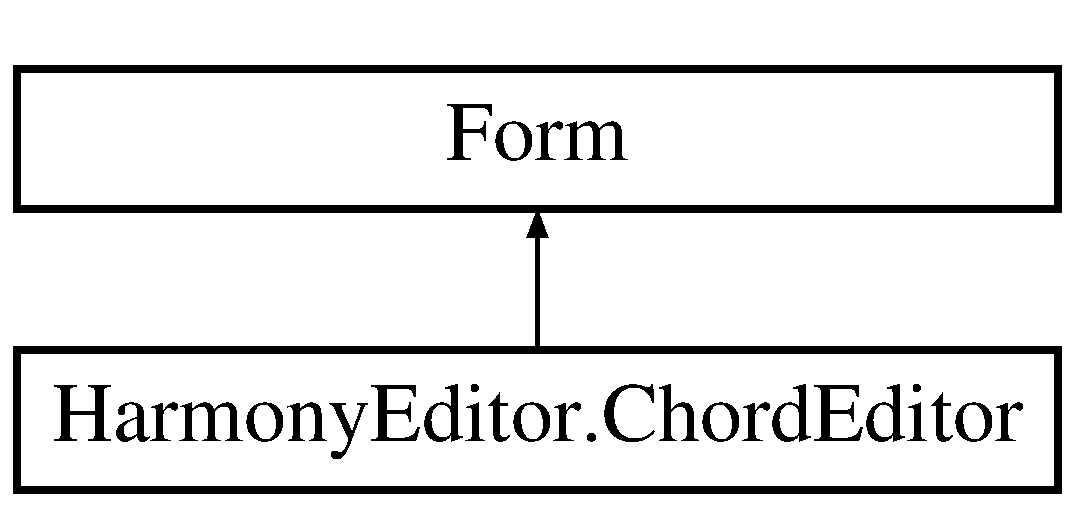
\includegraphics[height=2.000000cm]{class_harmony_editor_1_1_chord_editor}
\end{center}
\end{figure}
\subsection*{Public Member Functions}
\begin{DoxyCompactItemize}
\item 
\hypertarget{class_harmony_editor_1_1_chord_editor_a700c141670055da86cc0503f39c9f9fe}{{\bfseries Chord\+Editor} (\hyperlink{class_periodic_chords_1_1_periodic_chord}{Periodic\+Chord} chord)}\label{class_harmony_editor_1_1_chord_editor_a700c141670055da86cc0503f39c9f9fe}

\end{DoxyCompactItemize}
\subsection*{Protected Member Functions}
\begin{DoxyCompactItemize}
\item 
override void \hyperlink{class_harmony_editor_1_1_chord_editor_af2ec925f93bfb82bb1f231552a0a8984}{Dispose} (bool disposing)
\begin{DoxyCompactList}\small\item\em Clean up any resources being used. \end{DoxyCompactList}\end{DoxyCompactItemize}
\subsection*{Properties}
\begin{DoxyCompactItemize}
\item 
\hypertarget{class_harmony_editor_1_1_chord_editor_ab8995a7871bf3be74b4a5d7dc8a33adb}{\hyperlink{class_periodic_chords_1_1_periodic_chord}{Periodic\+Chord} {\bfseries Result}\hspace{0.3cm}{\ttfamily  \mbox{[}get\mbox{]}}}\label{class_harmony_editor_1_1_chord_editor_ab8995a7871bf3be74b4a5d7dc8a33adb}

\item 
\hypertarget{class_harmony_editor_1_1_chord_editor_aa8766f1fe7d848603601382355183050}{bool {\bfseries Default}\hspace{0.3cm}{\ttfamily  \mbox{[}get\mbox{]}}}\label{class_harmony_editor_1_1_chord_editor_aa8766f1fe7d848603601382355183050}

\item 
\hypertarget{class_harmony_editor_1_1_chord_editor_a89fb843b999fccf64ad62abd09e9db00}{bool {\bfseries Ok\+Clicked}\hspace{0.3cm}{\ttfamily  \mbox{[}get\mbox{]}}}\label{class_harmony_editor_1_1_chord_editor_a89fb843b999fccf64ad62abd09e9db00}

\end{DoxyCompactItemize}


\subsection{Member Function Documentation}
\hypertarget{class_harmony_editor_1_1_chord_editor_af2ec925f93bfb82bb1f231552a0a8984}{\index{Harmony\+Editor\+::\+Chord\+Editor@{Harmony\+Editor\+::\+Chord\+Editor}!Dispose@{Dispose}}
\index{Dispose@{Dispose}!Harmony\+Editor\+::\+Chord\+Editor@{Harmony\+Editor\+::\+Chord\+Editor}}
\subsubsection[{Dispose}]{\setlength{\rightskip}{0pt plus 5cm}override void Harmony\+Editor.\+Chord\+Editor.\+Dispose (
\begin{DoxyParamCaption}
\item[{bool}]{disposing}
\end{DoxyParamCaption}
)\hspace{0.3cm}{\ttfamily [protected]}}}\label{class_harmony_editor_1_1_chord_editor_af2ec925f93bfb82bb1f231552a0a8984}


Clean up any resources being used. 


\begin{DoxyParams}{Parameters}
{\em disposing} & true if managed resources should be disposed; otherwise, false.\\
\hline
\end{DoxyParams}


The documentation for this class was generated from the following files\+:\begin{DoxyCompactItemize}
\item 
C\+:/\+Users/praktykant/\+Documents/\+Git\+Hub/\+Harmony-\/\+Simulation/\+Harmony\+Editor/\+Harmony\+Editor/\+Windows/Chord\+Editor.\+cs\item 
C\+:/\+Users/praktykant/\+Documents/\+Git\+Hub/\+Harmony-\/\+Simulation/\+Harmony\+Editor/\+Harmony\+Editor/\+Windows/Chord\+Editor.\+Designer.\+cs\end{DoxyCompactItemize}

\hypertarget{class_harmony_editor_1_1_draggable_component}{\section{Harmony\+Editor.\+Draggable\+Component Class Reference}
\label{class_harmony_editor_1_1_draggable_component}\index{Harmony\+Editor.\+Draggable\+Component@{Harmony\+Editor.\+Draggable\+Component}}
}
Inheritance diagram for Harmony\+Editor.\+Draggable\+Component\+:\begin{figure}[H]
\begin{center}
\leavevmode
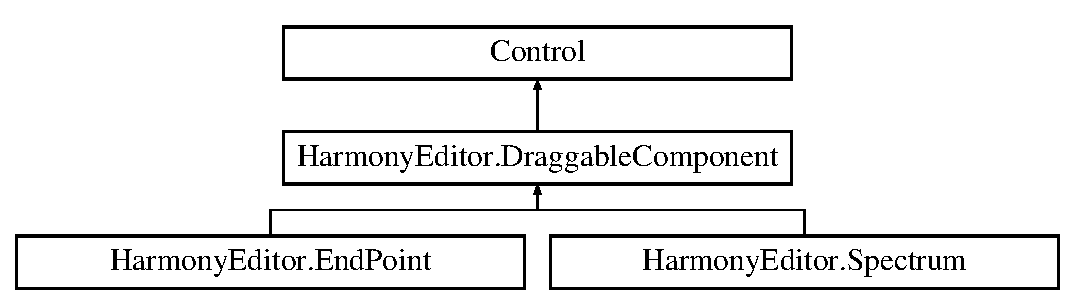
\includegraphics[height=3.000000cm]{class_harmony_editor_1_1_draggable_component}
\end{center}
\end{figure}
\subsection*{Protected Member Functions}
\begin{DoxyCompactItemize}
\item 
\hypertarget{class_harmony_editor_1_1_draggable_component_ae2ba64093df9694d6e00079865700990}{override void {\bfseries On\+Mouse\+Down} (Mouse\+Event\+Args e)}\label{class_harmony_editor_1_1_draggable_component_ae2ba64093df9694d6e00079865700990}

\item 
\hypertarget{class_harmony_editor_1_1_draggable_component_aa923ef4da4c16938c9ff8a17dc48bdef}{override void {\bfseries On\+Mouse\+Move} (Mouse\+Event\+Args e)}\label{class_harmony_editor_1_1_draggable_component_aa923ef4da4c16938c9ff8a17dc48bdef}

\item 
\hypertarget{class_harmony_editor_1_1_draggable_component_a346b8728cf21f558414a8a08593ccc76}{override void {\bfseries On\+Mouse\+Up} (Mouse\+Event\+Args e)}\label{class_harmony_editor_1_1_draggable_component_a346b8728cf21f558414a8a08593ccc76}

\item 
override void \hyperlink{class_harmony_editor_1_1_draggable_component_ae8db8c1a141eb59a081904bc7a7d1cfe}{Dispose} (bool disposing)
\begin{DoxyCompactList}\small\item\em Clean up any resources being used. \end{DoxyCompactList}\end{DoxyCompactItemize}
\subsection*{Protected Attributes}
\begin{DoxyCompactItemize}
\item 
\hypertarget{class_harmony_editor_1_1_draggable_component_a4c7a186d04e6c809b3bf131afb78ddec}{bool {\bfseries \+\_\+is\+Dragging} = false}\label{class_harmony_editor_1_1_draggable_component_a4c7a186d04e6c809b3bf131afb78ddec}

\item 
\hypertarget{class_harmony_editor_1_1_draggable_component_a44fe8fb455c60aafec61e34ac134ffe6}{int {\bfseries \+\_\+m\+X} = 0}\label{class_harmony_editor_1_1_draggable_component_a44fe8fb455c60aafec61e34ac134ffe6}

\item 
\hypertarget{class_harmony_editor_1_1_draggable_component_a501e29b4dbd7d0c057693417e3db1b4f}{int {\bfseries \+\_\+m\+Y} = 0}\label{class_harmony_editor_1_1_draggable_component_a501e29b4dbd7d0c057693417e3db1b4f}

\item 
\hypertarget{class_harmony_editor_1_1_draggable_component_ae5523a4fcf1f34720a0c53212368ab1d}{int {\bfseries \+\_\+\+D\+Dradius} = 40}\label{class_harmony_editor_1_1_draggable_component_ae5523a4fcf1f34720a0c53212368ab1d}

\end{DoxyCompactItemize}
\subsection*{Properties}
\begin{DoxyCompactItemize}
\item 
\hypertarget{class_harmony_editor_1_1_draggable_component_a890ba1aedc8bcdc12ea47e36a8371043}{bool {\bfseries Allow\+Drag}\hspace{0.3cm}{\ttfamily  \mbox{[}get, set\mbox{]}}}\label{class_harmony_editor_1_1_draggable_component_a890ba1aedc8bcdc12ea47e36a8371043}

\item 
\hypertarget{class_harmony_editor_1_1_draggable_component_a62a9adb83be766a0ec4d309bcee8b9ae}{bool {\bfseries Selected}\hspace{0.3cm}{\ttfamily  \mbox{[}get, set\mbox{]}}}\label{class_harmony_editor_1_1_draggable_component_a62a9adb83be766a0ec4d309bcee8b9ae}

\end{DoxyCompactItemize}


\subsection{Member Function Documentation}
\hypertarget{class_harmony_editor_1_1_draggable_component_ae8db8c1a141eb59a081904bc7a7d1cfe}{\index{Harmony\+Editor\+::\+Draggable\+Component@{Harmony\+Editor\+::\+Draggable\+Component}!Dispose@{Dispose}}
\index{Dispose@{Dispose}!Harmony\+Editor\+::\+Draggable\+Component@{Harmony\+Editor\+::\+Draggable\+Component}}
\subsubsection[{Dispose}]{\setlength{\rightskip}{0pt plus 5cm}override void Harmony\+Editor.\+Draggable\+Component.\+Dispose (
\begin{DoxyParamCaption}
\item[{bool}]{disposing}
\end{DoxyParamCaption}
)\hspace{0.3cm}{\ttfamily [protected]}}}\label{class_harmony_editor_1_1_draggable_component_ae8db8c1a141eb59a081904bc7a7d1cfe}


Clean up any resources being used. 


\begin{DoxyParams}{Parameters}
{\em disposing} & true if managed resources should be disposed; otherwise, false.\\
\hline
\end{DoxyParams}


The documentation for this class was generated from the following files\+:\begin{DoxyCompactItemize}
\item 
C\+:/\+Users/praktykant/\+Documents/\+Git\+Hub/\+Harmony-\/\+Simulation/\+Harmony\+Editor/\+Harmony\+Editor/\+Controls/Draggable\+Component.\+cs\item 
C\+:/\+Users/praktykant/\+Documents/\+Git\+Hub/\+Harmony-\/\+Simulation/\+Harmony\+Editor/\+Harmony\+Editor/\+Controls/Draggable\+Component.\+Designer.\+cs\end{DoxyCompactItemize}

\hypertarget{class_harmony_editor_1_1_end_point}{\section{Harmony\+Editor.\+End\+Point Class Reference}
\label{class_harmony_editor_1_1_end_point}\index{Harmony\+Editor.\+End\+Point@{Harmony\+Editor.\+End\+Point}}
}
Inheritance diagram for Harmony\+Editor.\+End\+Point\+:\begin{figure}[H]
\begin{center}
\leavevmode
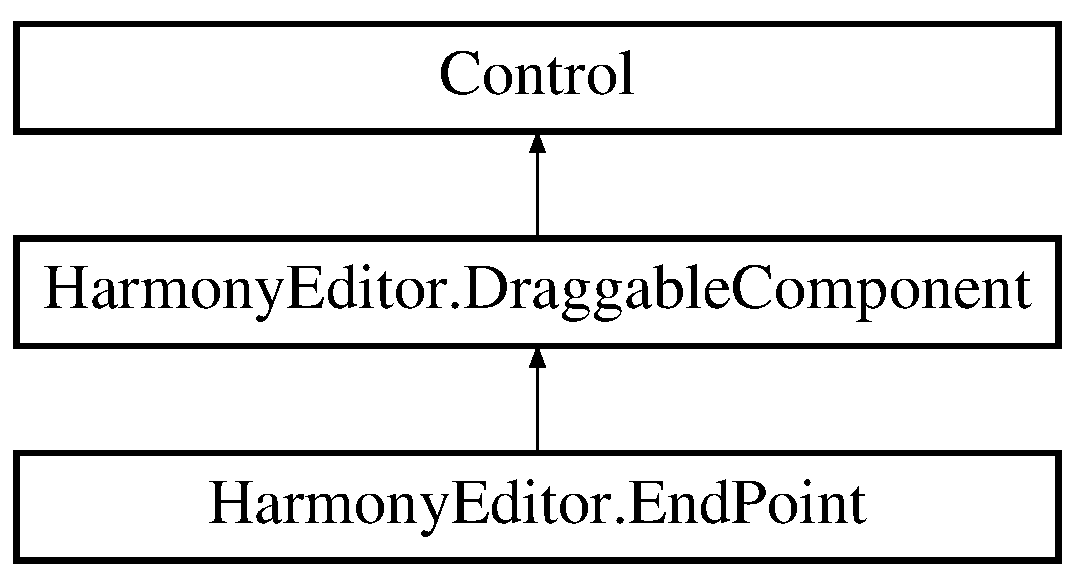
\includegraphics[height=3.000000cm]{class_harmony_editor_1_1_end_point}
\end{center}
\end{figure}
\subsection*{Public Member Functions}
\begin{DoxyCompactItemize}
\item 
\hypertarget{class_harmony_editor_1_1_end_point_a455c66b888889ee0285baf14e40195a6}{{\bfseries End\+Point} (int width, int height)}\label{class_harmony_editor_1_1_end_point_a455c66b888889ee0285baf14e40195a6}

\end{DoxyCompactItemize}
\subsection*{Protected Member Functions}
\begin{DoxyCompactItemize}
\item 
\hypertarget{class_harmony_editor_1_1_end_point_a2e12f6940c3b26e0d6d24420763454a6}{override void {\bfseries On\+Paint} (Paint\+Event\+Args pe)}\label{class_harmony_editor_1_1_end_point_a2e12f6940c3b26e0d6d24420763454a6}

\end{DoxyCompactItemize}
\subsection*{Additional Inherited Members}


The documentation for this class was generated from the following file\+:\begin{DoxyCompactItemize}
\item 
C\+:/\+Users/praktykant/\+Documents/\+Git\+Hub/\+Harmony-\/\+Simulation/\+Harmony\+Editor/\+Harmony\+Editor/\+Controls/End\+Point.\+cs\end{DoxyCompactItemize}

\hypertarget{class_periodic_chords_1_1_herz_periodic_chord}{\section{Periodic\+Chords.\+Herz\+Periodic\+Chord Class Reference}
\label{class_periodic_chords_1_1_herz_periodic_chord}\index{Periodic\+Chords.\+Herz\+Periodic\+Chord@{Periodic\+Chords.\+Herz\+Periodic\+Chord}}
}
Inheritance diagram for Periodic\+Chords.\+Herz\+Periodic\+Chord\+:\begin{figure}[H]
\begin{center}
\leavevmode
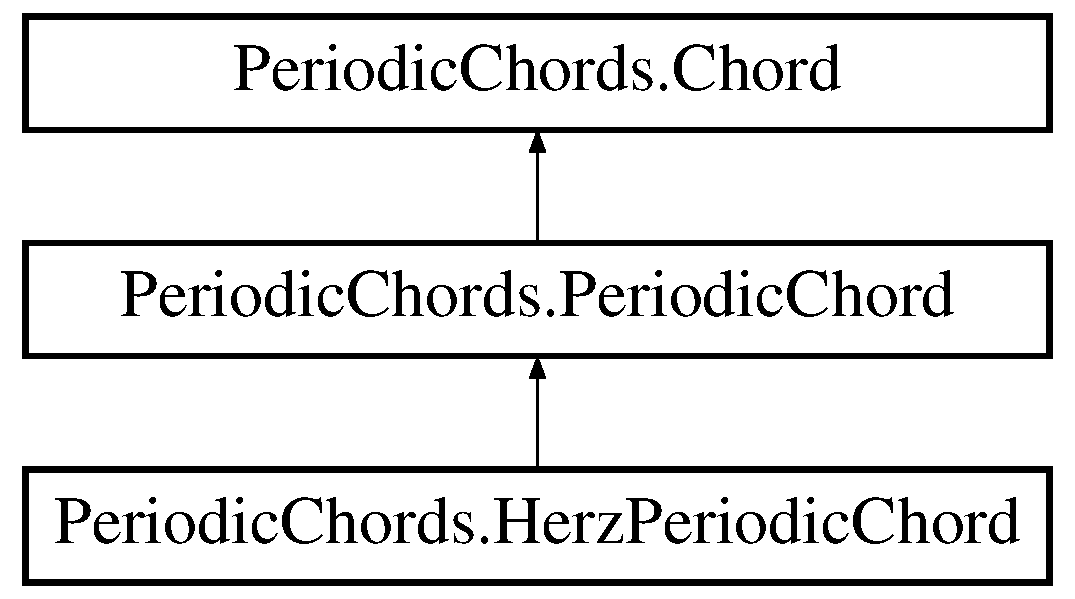
\includegraphics[height=3.000000cm]{class_periodic_chords_1_1_herz_periodic_chord}
\end{center}
\end{figure}
\subsection*{Properties}
\begin{DoxyCompactItemize}
\item 
\hypertarget{class_periodic_chords_1_1_herz_periodic_chord_a0af7958a9c11aaa08e607af318c72b34}{override double\mbox{[}$\,$\mbox{]} {\bfseries Frequencies}\hspace{0.3cm}{\ttfamily  \mbox{[}get\mbox{]}}}\label{class_periodic_chords_1_1_herz_periodic_chord_a0af7958a9c11aaa08e607af318c72b34}

\item 
\hypertarget{class_periodic_chords_1_1_herz_periodic_chord_acab810914d959ee196a210e5e4a34383}{override double\mbox{[}$\,$\mbox{]} {\bfseries Notes}\hspace{0.3cm}{\ttfamily  \mbox{[}get\mbox{]}}}\label{class_periodic_chords_1_1_herz_periodic_chord_acab810914d959ee196a210e5e4a34383}

\end{DoxyCompactItemize}
\subsection*{Additional Inherited Members}


The documentation for this class was generated from the following file\+:\begin{DoxyCompactItemize}
\item 
C\+:/\+Users/praktykant/\+Documents/\+Git\+Hub/\+Harmony-\/\+Simulation/\+Harmony\+Editor/\+Periodic\+Chords/Periodic\+Chord.\+cs\end{DoxyCompactItemize}

\hypertarget{class_periodic_chords_1_1_herz_simple_chord}{\section{Periodic\+Chords.\+Herz\+Simple\+Chord Class Reference}
\label{class_periodic_chords_1_1_herz_simple_chord}\index{Periodic\+Chords.\+Herz\+Simple\+Chord@{Periodic\+Chords.\+Herz\+Simple\+Chord}}
}
Inheritance diagram for Periodic\+Chords.\+Herz\+Simple\+Chord\+:\begin{figure}[H]
\begin{center}
\leavevmode
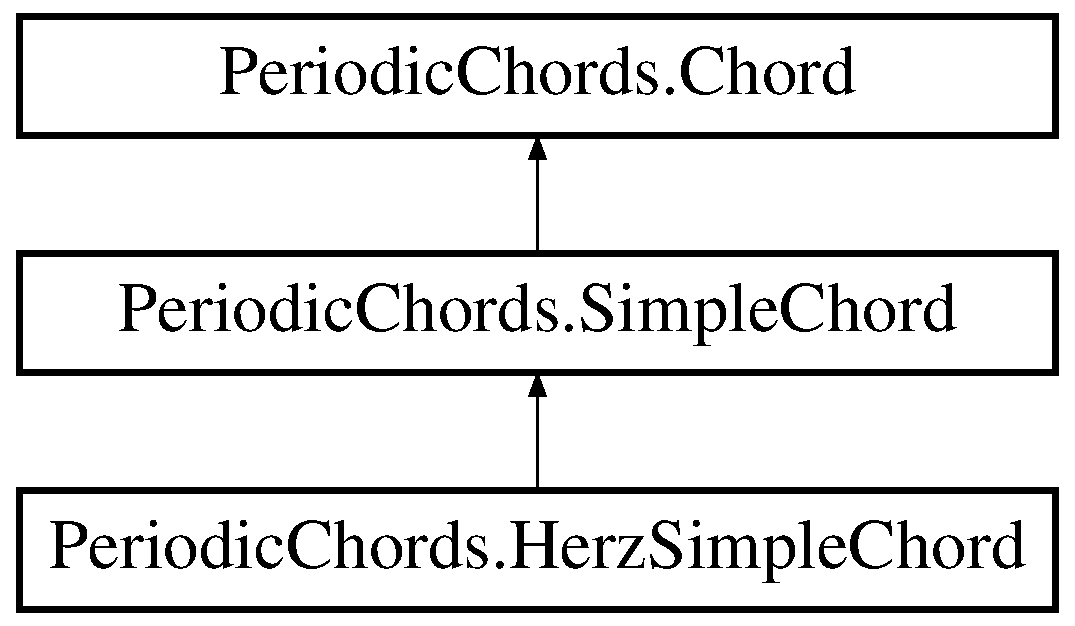
\includegraphics[height=3.000000cm]{class_periodic_chords_1_1_herz_simple_chord}
\end{center}
\end{figure}
\subsection*{Properties}
\begin{DoxyCompactItemize}
\item 
\hypertarget{class_periodic_chords_1_1_herz_simple_chord_ae121de3de908e42b6814eb80661ba623}{override double\mbox{[}$\,$\mbox{]} {\bfseries Frequencies}\hspace{0.3cm}{\ttfamily  \mbox{[}get\mbox{]}}}\label{class_periodic_chords_1_1_herz_simple_chord_ae121de3de908e42b6814eb80661ba623}

\item 
\hypertarget{class_periodic_chords_1_1_herz_simple_chord_a84ce2c5b4d290b3cad788f15cf1314fb}{override double\mbox{[}$\,$\mbox{]} {\bfseries Notes}\hspace{0.3cm}{\ttfamily  \mbox{[}get\mbox{]}}}\label{class_periodic_chords_1_1_herz_simple_chord_a84ce2c5b4d290b3cad788f15cf1314fb}

\end{DoxyCompactItemize}
\subsection*{Additional Inherited Members}


The documentation for this class was generated from the following file\+:\begin{DoxyCompactItemize}
\item 
C\+:/\+Users/praktykant/\+Documents/\+Git\+Hub/\+Harmony-\/\+Simulation/\+Harmony\+Editor/\+Periodic\+Chords/Simple\+Chord.\+cs\end{DoxyCompactItemize}

\hypertarget{class_populo_application_1_1_main_window}{\section{Populo\+Application.\+Main\+Window Class Reference}
\label{class_populo_application_1_1_main_window}\index{Populo\+Application.\+Main\+Window@{Populo\+Application.\+Main\+Window}}
}


Main window of \hyperlink{namespace_populo_application}{Populo\+Application}  


Inheritance diagram for Populo\+Application.\+Main\+Window\+:\begin{figure}[H]
\begin{center}
\leavevmode
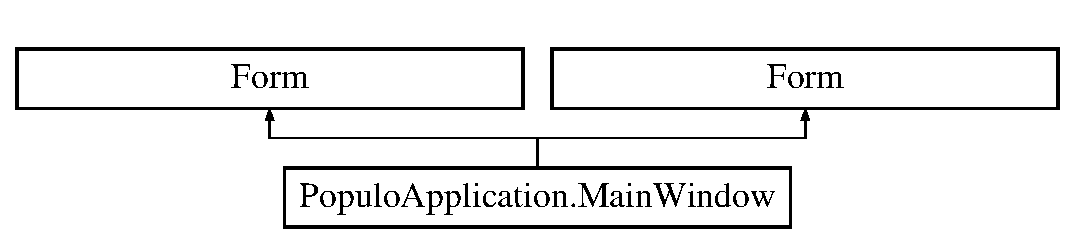
\includegraphics[height=2.000000cm]{class_populo_application_1_1_main_window}
\end{center}
\end{figure}
\subsection*{Public Member Functions}
\begin{DoxyCompactItemize}
\item 
\hyperlink{class_populo_application_1_1_main_window_a2d0281fd0fad2e4077e839e06386bf27}{Main\+Window} ()
\begin{DoxyCompactList}\small\item\em Constructor of \hyperlink{class_populo_application_1_1_main_window}{Main\+Window} \end{DoxyCompactList}\item 
void \hyperlink{class_populo_application_1_1_main_window_a51aeb83f39fcbff00c395c49bd318fdf}{Refresh\+Simulation\+Controls} ()
\begin{DoxyCompactList}\small\item\em Method used for refreshing controls in main window. Can be used outside the class. Sets the color of progress control\+: green-\/ if simulation is running, red-\/ otherwise \end{DoxyCompactList}\item 
void \hyperlink{class_populo_application_1_1_main_window_a080f38423250539baf475a7cc6124e68}{Save\+Parameters} ()
\begin{DoxyCompactList}\small\item\em Method used for saving parameters from application to Simulation \end{DoxyCompactList}\end{DoxyCompactItemize}
\subsection*{Protected Member Functions}
\begin{DoxyCompactItemize}
\item 
override void \hyperlink{class_populo_application_1_1_main_window_a0aada52294ee41ee42a948f1acf23ec9}{Dispose} (bool disposing)
\begin{DoxyCompactList}\small\item\em Clean up any resources being used. \end{DoxyCompactList}\end{DoxyCompactItemize}
\subsection*{Properties}
\begin{DoxyCompactItemize}
\item 
List$<$ List$<$ \hyperlink{class_periodic_chords_1_1_pitch_data}{Pitch\+Data} $>$ $>$ \hyperlink{class_populo_application_1_1_main_window_a65f0c59f093d0cda3bcbb3401a25f2d1}{Accord}\hspace{0.3cm}{\ttfamily  \mbox{[}get, set\mbox{]}}
\begin{DoxyCompactList}\small\item\em Public property for setting accord \end{DoxyCompactList}\end{DoxyCompactItemize}


\subsection{Detailed Description}
Main window of \hyperlink{namespace_populo_application}{Populo\+Application} 



\subsection{Constructor \& Destructor Documentation}
\hypertarget{class_populo_application_1_1_main_window_a2d0281fd0fad2e4077e839e06386bf27}{\index{Populo\+Application\+::\+Main\+Window@{Populo\+Application\+::\+Main\+Window}!Main\+Window@{Main\+Window}}
\index{Main\+Window@{Main\+Window}!Populo\+Application\+::\+Main\+Window@{Populo\+Application\+::\+Main\+Window}}
\subsubsection[{Main\+Window}]{\setlength{\rightskip}{0pt plus 5cm}Populo\+Application.\+Main\+Window.\+Main\+Window (
\begin{DoxyParamCaption}
{}
\end{DoxyParamCaption}
)}}\label{class_populo_application_1_1_main_window_a2d0281fd0fad2e4077e839e06386bf27}


Constructor of \hyperlink{class_populo_application_1_1_main_window}{Main\+Window} 



\subsection{Member Function Documentation}
\hypertarget{class_populo_application_1_1_main_window_a0aada52294ee41ee42a948f1acf23ec9}{\index{Populo\+Application\+::\+Main\+Window@{Populo\+Application\+::\+Main\+Window}!Dispose@{Dispose}}
\index{Dispose@{Dispose}!Populo\+Application\+::\+Main\+Window@{Populo\+Application\+::\+Main\+Window}}
\subsubsection[{Dispose}]{\setlength{\rightskip}{0pt plus 5cm}override void Populo\+Application.\+Main\+Window.\+Dispose (
\begin{DoxyParamCaption}
\item[{bool}]{disposing}
\end{DoxyParamCaption}
)\hspace{0.3cm}{\ttfamily [protected]}}}\label{class_populo_application_1_1_main_window_a0aada52294ee41ee42a948f1acf23ec9}


Clean up any resources being used. 


\begin{DoxyParams}{Parameters}
{\em disposing} & true if managed resources should be disposed; otherwise, false.\\
\hline
\end{DoxyParams}
\hypertarget{class_populo_application_1_1_main_window_a51aeb83f39fcbff00c395c49bd318fdf}{\index{Populo\+Application\+::\+Main\+Window@{Populo\+Application\+::\+Main\+Window}!Refresh\+Simulation\+Controls@{Refresh\+Simulation\+Controls}}
\index{Refresh\+Simulation\+Controls@{Refresh\+Simulation\+Controls}!Populo\+Application\+::\+Main\+Window@{Populo\+Application\+::\+Main\+Window}}
\subsubsection[{Refresh\+Simulation\+Controls}]{\setlength{\rightskip}{0pt plus 5cm}void Populo\+Application.\+Main\+Window.\+Refresh\+Simulation\+Controls (
\begin{DoxyParamCaption}
{}
\end{DoxyParamCaption}
)}}\label{class_populo_application_1_1_main_window_a51aeb83f39fcbff00c395c49bd318fdf}


Method used for refreshing controls in main window. Can be used outside the class. Sets the color of progress control\+: green-\/ if simulation is running, red-\/ otherwise 

\hypertarget{class_populo_application_1_1_main_window_a080f38423250539baf475a7cc6124e68}{\index{Populo\+Application\+::\+Main\+Window@{Populo\+Application\+::\+Main\+Window}!Save\+Parameters@{Save\+Parameters}}
\index{Save\+Parameters@{Save\+Parameters}!Populo\+Application\+::\+Main\+Window@{Populo\+Application\+::\+Main\+Window}}
\subsubsection[{Save\+Parameters}]{\setlength{\rightskip}{0pt plus 5cm}void Populo\+Application.\+Main\+Window.\+Save\+Parameters (
\begin{DoxyParamCaption}
{}
\end{DoxyParamCaption}
)}}\label{class_populo_application_1_1_main_window_a080f38423250539baf475a7cc6124e68}


Method used for saving parameters from application to Simulation 



\subsection{Property Documentation}
\hypertarget{class_populo_application_1_1_main_window_a65f0c59f093d0cda3bcbb3401a25f2d1}{\index{Populo\+Application\+::\+Main\+Window@{Populo\+Application\+::\+Main\+Window}!Accord@{Accord}}
\index{Accord@{Accord}!Populo\+Application\+::\+Main\+Window@{Populo\+Application\+::\+Main\+Window}}
\subsubsection[{Accord}]{\setlength{\rightskip}{0pt plus 5cm}List$<$List$<${\bf Pitch\+Data}$>$ $>$ Populo\+Application.\+Main\+Window.\+Accord\hspace{0.3cm}{\ttfamily [get]}, {\ttfamily [set]}}}\label{class_populo_application_1_1_main_window_a65f0c59f093d0cda3bcbb3401a25f2d1}


Public property for setting accord 



The documentation for this class was generated from the following files\+:\begin{DoxyCompactItemize}
\item 
C\+:/\+Users/praktykant/\+Documents/\+Git\+Hub/\+Harmony-\/\+Simulation/\+Populo/\+Populo\+Application/Main\+Window.\+cs\item 
C\+:/\+Users/praktykant/\+Documents/\+Git\+Hub/\+Harmony-\/\+Simulation/\+Populo/\+Populo\+Application/\+Windows/Main\+Window.\+Designer.\+cs\end{DoxyCompactItemize}

\hypertarget{class_harmony_editor_1_1_main_window}{\section{Harmony\+Editor.\+Main\+Window Class Reference}
\label{class_harmony_editor_1_1_main_window}\index{Harmony\+Editor.\+Main\+Window@{Harmony\+Editor.\+Main\+Window}}
}


Main window of application.  


Inheritance diagram for Harmony\+Editor.\+Main\+Window\+:\begin{figure}[H]
\begin{center}
\leavevmode
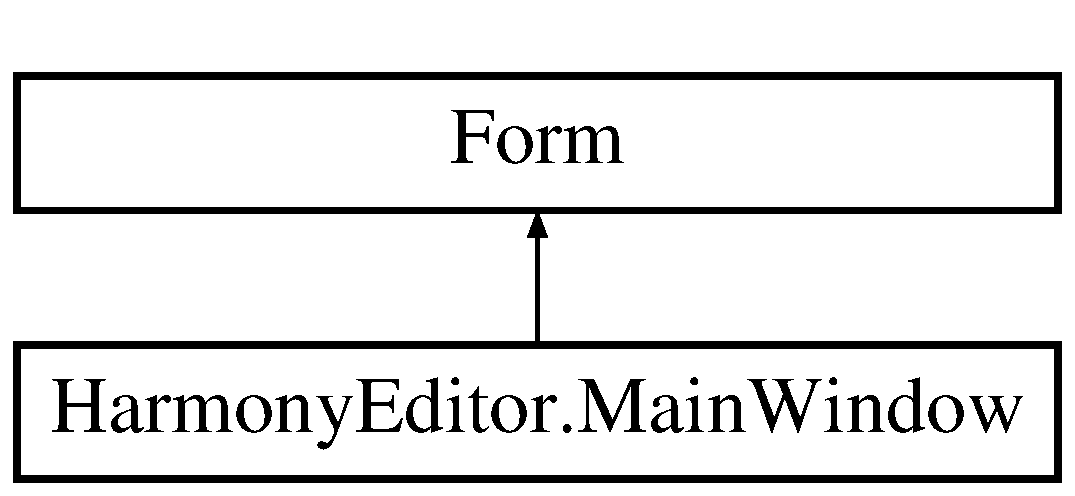
\includegraphics[height=2.000000cm]{class_harmony_editor_1_1_main_window}
\end{center}
\end{figure}
\subsection*{Protected Member Functions}
\begin{DoxyCompactItemize}
\item 
\hypertarget{class_harmony_editor_1_1_main_window_aa6f21116b893261c47e338a654bd1a25}{override void {\bfseries On\+Closed} (Event\+Args e)}\label{class_harmony_editor_1_1_main_window_aa6f21116b893261c47e338a654bd1a25}

\item 
override void \hyperlink{class_harmony_editor_1_1_main_window_a72a09ae6274e5b02720d28f5c12d7fa4}{Dispose} (bool disposing)
\begin{DoxyCompactList}\small\item\em Clean up any resources being used. \end{DoxyCompactList}\end{DoxyCompactItemize}


\subsection{Detailed Description}
Main window of application. 



\subsection{Member Function Documentation}
\hypertarget{class_harmony_editor_1_1_main_window_a72a09ae6274e5b02720d28f5c12d7fa4}{\index{Harmony\+Editor\+::\+Main\+Window@{Harmony\+Editor\+::\+Main\+Window}!Dispose@{Dispose}}
\index{Dispose@{Dispose}!Harmony\+Editor\+::\+Main\+Window@{Harmony\+Editor\+::\+Main\+Window}}
\subsubsection[{Dispose}]{\setlength{\rightskip}{0pt plus 5cm}override void Harmony\+Editor.\+Main\+Window.\+Dispose (
\begin{DoxyParamCaption}
\item[{bool}]{disposing}
\end{DoxyParamCaption}
)\hspace{0.3cm}{\ttfamily [protected]}}}\label{class_harmony_editor_1_1_main_window_a72a09ae6274e5b02720d28f5c12d7fa4}


Clean up any resources being used. 


\begin{DoxyParams}{Parameters}
{\em disposing} & true if managed resources should be disposed; otherwise, false.\\
\hline
\end{DoxyParams}


The documentation for this class was generated from the following files\+:\begin{DoxyCompactItemize}
\item 
C\+:/\+Users/praktykant/\+Documents/\+Git\+Hub/\+Harmony-\/\+Simulation/\+Harmony\+Editor/\+Harmony\+Editor/\+Windows/Main\+Window.\+cs\item 
C\+:/\+Users/praktykant/\+Documents/\+Git\+Hub/\+Harmony-\/\+Simulation/\+Harmony\+Editor/\+Harmony\+Editor/\+Windows/Main\+Window.\+Designer.\+cs\end{DoxyCompactItemize}

\hypertarget{class_populo_application_1_1_melody_sequence}{\section{Populo\+Application.\+Melody\+Sequence Class Reference}
\label{class_populo_application_1_1_melody_sequence}\index{Populo\+Application.\+Melody\+Sequence@{Populo\+Application.\+Melody\+Sequence}}
}
\subsection*{Public Member Functions}
\begin{DoxyCompactItemize}
\item 
\hypertarget{class_populo_application_1_1_melody_sequence_a35e82799d15efa2f5ce0668f71d3f337}{void {\bfseries Tick} ()}\label{class_populo_application_1_1_melody_sequence_a35e82799d15efa2f5ce0668f71d3f337}

\item 
\hypertarget{class_populo_application_1_1_melody_sequence_a4624f6c1164392a3ff874ef30b242012}{void {\bfseries Add} (int i, Channel\+Message On, Channel\+Message Off)}\label{class_populo_application_1_1_melody_sequence_a4624f6c1164392a3ff874ef30b242012}

\item 
\hypertarget{class_populo_application_1_1_melody_sequence_a870dbd2bbe99ad90c586a55b242ea4c1}{void {\bfseries Simple\+Add} (int i, Channel\+Message On, Channel\+Message Off)}\label{class_populo_application_1_1_melody_sequence_a870dbd2bbe99ad90c586a55b242ea4c1}

\item 
\hypertarget{class_populo_application_1_1_melody_sequence_a696a610555c285ce7e60cd3bd7522742}{void {\bfseries Correct} ()}\label{class_populo_application_1_1_melody_sequence_a696a610555c285ce7e60cd3bd7522742}

\item 
\hypertarget{class_populo_application_1_1_melody_sequence_afcc6aff8580df3f8076b6629d166ef62}{{\bfseries Melody\+Sequence} (Output\+Device o, \hyperlink{class_populo_application_1_1_m_i_d_i_player}{M\+I\+D\+I\+Player} player)}\label{class_populo_application_1_1_melody_sequence_afcc6aff8580df3f8076b6629d166ef62}

\item 
\hypertarget{class_populo_application_1_1_melody_sequence_acb2aff6b6410fc54cba4b2a5f8fe9e64}{void {\bfseries Clean} ()}\label{class_populo_application_1_1_melody_sequence_acb2aff6b6410fc54cba4b2a5f8fe9e64}

\item 
\hypertarget{class_populo_application_1_1_melody_sequence_a3f8127362fd77e2c662cf0bd5a300de8}{void {\bfseries Clear} ()}\label{class_populo_application_1_1_melody_sequence_a3f8127362fd77e2c662cf0bd5a300de8}

\end{DoxyCompactItemize}


The documentation for this class was generated from the following file\+:\begin{DoxyCompactItemize}
\item 
C\+:/\+Users/praktykant/\+Documents/\+Git\+Hub/\+Harmony-\/\+Simulation/\+Populo/\+Populo\+Application/\+Melody/\+M\+I\+D\+I/Melody\+Sequence.\+cs\end{DoxyCompactItemize}

\hypertarget{class_music_population_1_1_member}{\section{Music\+Population.\+Member Class Reference}
\label{class_music_population_1_1_member}\index{Music\+Population.\+Member@{Music\+Population.\+Member}}
}


Each class representing member should be inherit this abstract class.  


Inheritance diagram for Music\+Population.\+Member\+:\begin{figure}[H]
\begin{center}
\leavevmode
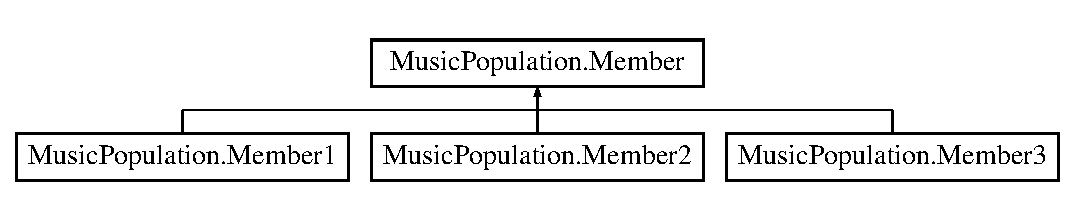
\includegraphics[height=2.000000cm]{class_music_population_1_1_member}
\end{center}
\end{figure}
\subsection*{Public Member Functions}
\begin{DoxyCompactItemize}
\item 
\hypertarget{class_music_population_1_1_member_ac82cc845ee466649dc698f60a20043c9}{{\bfseries Member} (Random rand\+Context)}\label{class_music_population_1_1_member_ac82cc845ee466649dc698f60a20043c9}

\item 
\hypertarget{class_music_population_1_1_member_a240df0f16bc7879f56f50d4eb00352b5}{Tuple$<$ int, int\mbox{[},\mbox{]}$>$ {\bfseries Clone\+Parameters} ()}\label{class_music_population_1_1_member_a240df0f16bc7879f56f50d4eb00352b5}

\item 
abstract int \hyperlink{class_music_population_1_1_member_a238549ad669c4f8eda036e608beba422}{Rank} ()
\begin{DoxyCompactList}\small\item\em Rank of the member. \end{DoxyCompactList}\item 
abstract void \hyperlink{class_music_population_1_1_member_affe5eeed6ac4b042d5729991f0c39eba}{Mutate} (Random rand\+Context)
\begin{DoxyCompactList}\small\item\em Method responsible for member mutation. \end{DoxyCompactList}\item 
abstract void \hyperlink{class_music_population_1_1_member_a99042d0181ef0e48ad71d45313a176b6}{Influence} (\hyperlink{class_music_population_1_1_member}{Member} influencer, Random rand\+Context)
\begin{DoxyCompactList}\small\item\em Method responible for influencing individual. \end{DoxyCompactList}\item 
abstract \hyperlink{class_music_population_1_1_member}{Member} \hyperlink{class_music_population_1_1_member_af310ebdf342531da3edc882987574a16}{Clone} ()
\begin{DoxyCompactList}\small\item\em Clone member. \end{DoxyCompactList}\end{DoxyCompactItemize}
\subsection*{Protected Attributes}
\begin{DoxyCompactItemize}
\item 
\hypertarget{class_music_population_1_1_member_a2224ee5f8d0c6be59f85fd4e12f62741}{const int {\bfseries \+\_\+max\+Notes} = 255}\label{class_music_population_1_1_member_a2224ee5f8d0c6be59f85fd4e12f62741}

\end{DoxyCompactItemize}
\subsection*{Properties}
\begin{DoxyCompactItemize}
\item 
abstract int \hyperlink{class_music_population_1_1_member_af0a14babb0cd654761c327e927ebdd8d}{Number\+Of\+Notes}\hspace{0.3cm}{\ttfamily  \mbox{[}get\mbox{]}}
\begin{DoxyCompactList}\small\item\em Getter which returns number of notes. \end{DoxyCompactList}\item 
abstract int\mbox{[},\mbox{]} \hyperlink{class_music_population_1_1_member_a0c7562c7c67ef2fbdf57fa1c6cab9b70}{Notes}\hspace{0.3cm}{\ttfamily  \mbox{[}get\mbox{]}}
\begin{DoxyCompactList}\small\item\em Getter which returns array of notes. \end{DoxyCompactList}\end{DoxyCompactItemize}


\subsection{Detailed Description}
Each class representing member should be inherit this abstract class. 



\subsection{Member Function Documentation}
\hypertarget{class_music_population_1_1_member_af310ebdf342531da3edc882987574a16}{\index{Music\+Population\+::\+Member@{Music\+Population\+::\+Member}!Clone@{Clone}}
\index{Clone@{Clone}!Music\+Population\+::\+Member@{Music\+Population\+::\+Member}}
\subsubsection[{Clone}]{\setlength{\rightskip}{0pt plus 5cm}abstract {\bf Member} Music\+Population.\+Member.\+Clone (
\begin{DoxyParamCaption}
{}
\end{DoxyParamCaption}
)\hspace{0.3cm}{\ttfamily [pure virtual]}}}\label{class_music_population_1_1_member_af310ebdf342531da3edc882987574a16}


Clone member. 

\begin{DoxyReturn}{Returns}
copy of member
\end{DoxyReturn}


Implemented in \hyperlink{class_music_population_1_1_member2_a6e676c34e7af1ef9ffbbe68cfa38424f}{Music\+Population.\+Member2}, \hyperlink{class_music_population_1_1_member1_a6f3395ebd0d2c9ebe4834eeece0df200}{Music\+Population.\+Member1}, and \hyperlink{class_music_population_1_1_member3_ae37f77498a7c3ccec6b8531746eff1ec}{Music\+Population.\+Member3}.

\hypertarget{class_music_population_1_1_member_a99042d0181ef0e48ad71d45313a176b6}{\index{Music\+Population\+::\+Member@{Music\+Population\+::\+Member}!Influence@{Influence}}
\index{Influence@{Influence}!Music\+Population\+::\+Member@{Music\+Population\+::\+Member}}
\subsubsection[{Influence}]{\setlength{\rightskip}{0pt plus 5cm}abstract void Music\+Population.\+Member.\+Influence (
\begin{DoxyParamCaption}
\item[{{\bf Member}}]{influencer, }
\item[{Random}]{rand\+Context}
\end{DoxyParamCaption}
)\hspace{0.3cm}{\ttfamily [pure virtual]}}}\label{class_music_population_1_1_member_a99042d0181ef0e48ad71d45313a176b6}


Method responible for influencing individual. 


\begin{DoxyParams}{Parameters}
{\em influencer} & \hyperlink{class_music_population_1_1_member}{Member} which should be influenced\\
\hline
{\em rand\+Context} & random context\\
\hline
\end{DoxyParams}


Implemented in \hyperlink{class_music_population_1_1_member2_af413c7ad74a1979698f87fece3d02f3e}{Music\+Population.\+Member2}, \hyperlink{class_music_population_1_1_member3_aabde212fac4cd75573a3ed07b6522e1d}{Music\+Population.\+Member3}, and \hyperlink{class_music_population_1_1_member1_a1661d1dcac2b013fc77b669611648365}{Music\+Population.\+Member1}.

\hypertarget{class_music_population_1_1_member_affe5eeed6ac4b042d5729991f0c39eba}{\index{Music\+Population\+::\+Member@{Music\+Population\+::\+Member}!Mutate@{Mutate}}
\index{Mutate@{Mutate}!Music\+Population\+::\+Member@{Music\+Population\+::\+Member}}
\subsubsection[{Mutate}]{\setlength{\rightskip}{0pt plus 5cm}abstract void Music\+Population.\+Member.\+Mutate (
\begin{DoxyParamCaption}
\item[{Random}]{rand\+Context}
\end{DoxyParamCaption}
)\hspace{0.3cm}{\ttfamily [pure virtual]}}}\label{class_music_population_1_1_member_affe5eeed6ac4b042d5729991f0c39eba}


Method responsible for member mutation. 


\begin{DoxyParams}{Parameters}
{\em rand\+Context} & random context\\
\hline
\end{DoxyParams}


Implemented in \hyperlink{class_music_population_1_1_member1_ae0f96683b9fdfdfee1418f5b606b772c}{Music\+Population.\+Member1}, \hyperlink{class_music_population_1_1_member2_a30e51d2e61399a954b006cdbd6a37952}{Music\+Population.\+Member2}, and \hyperlink{class_music_population_1_1_member3_a443d06792b6e3566308a67d56e31c2d8}{Music\+Population.\+Member3}.

\hypertarget{class_music_population_1_1_member_a238549ad669c4f8eda036e608beba422}{\index{Music\+Population\+::\+Member@{Music\+Population\+::\+Member}!Rank@{Rank}}
\index{Rank@{Rank}!Music\+Population\+::\+Member@{Music\+Population\+::\+Member}}
\subsubsection[{Rank}]{\setlength{\rightskip}{0pt plus 5cm}abstract int Music\+Population.\+Member.\+Rank (
\begin{DoxyParamCaption}
{}
\end{DoxyParamCaption}
)\hspace{0.3cm}{\ttfamily [pure virtual]}}}\label{class_music_population_1_1_member_a238549ad669c4f8eda036e608beba422}


Rank of the member. 

\begin{DoxyReturn}{Returns}
integer representing rank of member
\end{DoxyReturn}


Implemented in \hyperlink{class_music_population_1_1_member1_acb90358a28ed446f2373fe0be35a8b01}{Music\+Population.\+Member1}, \hyperlink{class_music_population_1_1_member3_a3148bb13399637bb2cf2addf6d8ecbec}{Music\+Population.\+Member3}, and \hyperlink{class_music_population_1_1_member2_a1978ab05a86b98491d5ce7d201cfd4f0}{Music\+Population.\+Member2}.



\subsection{Property Documentation}
\hypertarget{class_music_population_1_1_member_a0c7562c7c67ef2fbdf57fa1c6cab9b70}{\index{Music\+Population\+::\+Member@{Music\+Population\+::\+Member}!Notes@{Notes}}
\index{Notes@{Notes}!Music\+Population\+::\+Member@{Music\+Population\+::\+Member}}
\subsubsection[{Notes}]{\setlength{\rightskip}{0pt plus 5cm}abstract int \mbox{[},\mbox{]} Music\+Population.\+Member.\+Notes\hspace{0.3cm}{\ttfamily [get]}}}\label{class_music_population_1_1_member_a0c7562c7c67ef2fbdf57fa1c6cab9b70}


Getter which returns array of notes. 

\hypertarget{class_music_population_1_1_member_af0a14babb0cd654761c327e927ebdd8d}{\index{Music\+Population\+::\+Member@{Music\+Population\+::\+Member}!Number\+Of\+Notes@{Number\+Of\+Notes}}
\index{Number\+Of\+Notes@{Number\+Of\+Notes}!Music\+Population\+::\+Member@{Music\+Population\+::\+Member}}
\subsubsection[{Number\+Of\+Notes}]{\setlength{\rightskip}{0pt plus 5cm}abstract int Music\+Population.\+Member.\+Number\+Of\+Notes\hspace{0.3cm}{\ttfamily [get]}}}\label{class_music_population_1_1_member_af0a14babb0cd654761c327e927ebdd8d}


Getter which returns number of notes. 



The documentation for this class was generated from the following file\+:\begin{DoxyCompactItemize}
\item 
C\+:/\+Users/praktykant/\+Documents/\+Git\+Hub/\+Harmony-\/\+Simulation/\+Populo/\+Music\+Population/\+Components/\+Member/Member.\+cs\end{DoxyCompactItemize}

\hypertarget{class_music_population_1_1_member1}{\section{Music\+Population.\+Member1 Class Reference}
\label{class_music_population_1_1_member1}\index{Music\+Population.\+Member1@{Music\+Population.\+Member1}}
}


Implementation of First phase member.  


Inheritance diagram for Music\+Population.\+Member1\+:\begin{figure}[H]
\begin{center}
\leavevmode
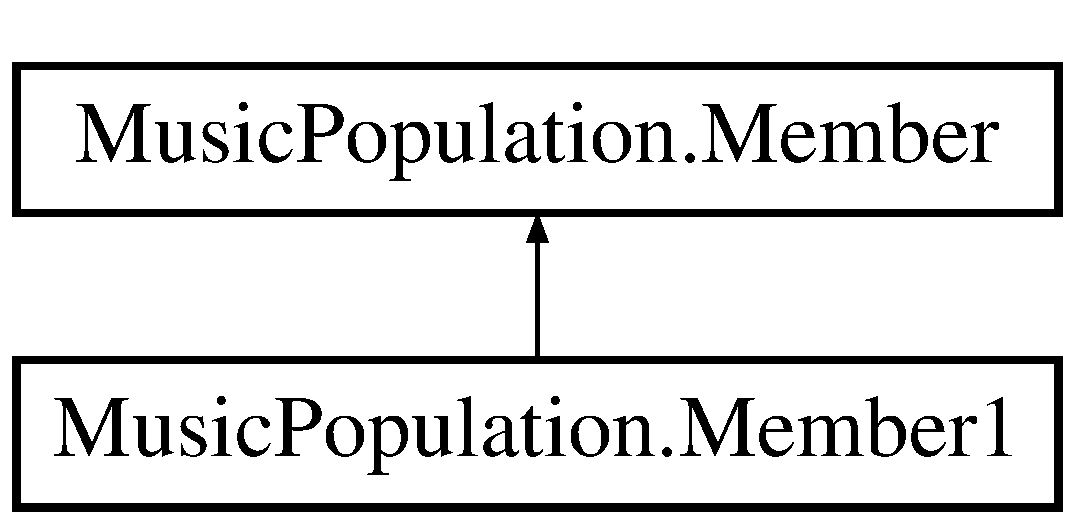
\includegraphics[height=2.000000cm]{class_music_population_1_1_member1}
\end{center}
\end{figure}
\subsection*{Public Member Functions}
\begin{DoxyCompactItemize}
\item 
\hypertarget{class_music_population_1_1_member1_aef8953b43d7d0f2e3433fef744e000e1}{{\bfseries Member1} (Random rand\+Context)}\label{class_music_population_1_1_member1_aef8953b43d7d0f2e3433fef744e000e1}

\item 
override void \hyperlink{class_music_population_1_1_member1_a1661d1dcac2b013fc77b669611648365}{Influence} (\hyperlink{class_music_population_1_1_member}{Member} influencer, Random rand\+Context)
\begin{DoxyCompactList}\small\item\em Method responible for influencing individual. \end{DoxyCompactList}\item 
override int \hyperlink{class_music_population_1_1_member1_acb90358a28ed446f2373fe0be35a8b01}{Rank} ()
\begin{DoxyCompactList}\small\item\em Rank of the member. \end{DoxyCompactList}\item 
override void \hyperlink{class_music_population_1_1_member1_ae0f96683b9fdfdfee1418f5b606b772c}{Mutate} (Random rand\+Context)
\begin{DoxyCompactList}\small\item\em Method responsible for member mutation. \end{DoxyCompactList}\item 
override \hyperlink{class_music_population_1_1_member}{Member} \hyperlink{class_music_population_1_1_member1_a6f3395ebd0d2c9ebe4834eeece0df200}{Clone} ()
\begin{DoxyCompactList}\small\item\em Clone member. \end{DoxyCompactList}\end{DoxyCompactItemize}
\subsection*{Static Public Attributes}
\begin{DoxyCompactItemize}
\item 
\hypertarget{class_music_population_1_1_member1_a86549329af1e5727450170dd02427441}{static int\mbox{[}$\,$\mbox{]} {\bfseries Modify\+Amount} = new int\mbox{[}$\,$\mbox{]} \{ 3,0, 5, 15 \}}\label{class_music_population_1_1_member1_a86549329af1e5727450170dd02427441}

\item 
\hypertarget{class_music_population_1_1_member1_a0002f60dd91b2de9928db76cc8c451ac}{static double\mbox{[}$\,$\mbox{]} {\bfseries Influence\+Amount} = new double\mbox{[}$\,$\mbox{]} \{ 0.\+2,0, 0.\+2, 0.\+2 \}}\label{class_music_population_1_1_member1_a0002f60dd91b2de9928db76cc8c451ac}

\item 
\hypertarget{class_music_population_1_1_member1_a4e7afb22ea6cb2153113540c781e176d}{static double\mbox{[}$\,$\mbox{]} {\bfseries Transpose\+Chance} = new double\mbox{[}$\,$\mbox{]} \{ 0.\+05,0, 0.\+05, 0.\+05 \}}\label{class_music_population_1_1_member1_a4e7afb22ea6cb2153113540c781e176d}

\item 
\hypertarget{class_music_population_1_1_member1_a996d5b04fb45c0618b2683fb726a285b}{static double\mbox{[}$\,$\mbox{]} {\bfseries Exchange\+Chance} = new double\mbox{[}$\,$\mbox{]} \{ 0.\+05,0, 0.\+05, 0.\+05 \}}\label{class_music_population_1_1_member1_a996d5b04fb45c0618b2683fb726a285b}

\item 
\hypertarget{class_music_population_1_1_member1_add664b4e7a4a867d45aaae94d27835d3}{static double\mbox{[}$\,$\mbox{]} {\bfseries Modify\+Chance} = new double\mbox{[}$\,$\mbox{]} \{ 0.\+05,0, 0.\+05, 0.\+05 \}}\label{class_music_population_1_1_member1_add664b4e7a4a867d45aaae94d27835d3}

\item 
\hypertarget{class_music_population_1_1_member1_a3c82666179e1b0b0974c6feef16814b6}{static double {\bfseries Growth\+Chance} = 0.\+05}\label{class_music_population_1_1_member1_a3c82666179e1b0b0974c6feef16814b6}

\item 
\hypertarget{class_music_population_1_1_member1_a7dfdefc75909d42031ec64873954024c}{static double {\bfseries Shrink\+Chance} = 0.\+05}\label{class_music_population_1_1_member1_a7dfdefc75909d42031ec64873954024c}

\item 
\hypertarget{class_music_population_1_1_member1_a11ccb48eebb833e95132a3fe2bd6b22b}{static int {\bfseries Preffered\+Length} = 10}\label{class_music_population_1_1_member1_a11ccb48eebb833e95132a3fe2bd6b22b}

\end{DoxyCompactItemize}
\subsection*{Protected Member Functions}
\begin{DoxyCompactItemize}
\item 
\hypertarget{class_music_population_1_1_member1_ae7d3efd24060a4c5d1a52368fa7aec79}{void {\bfseries Transpose} (uint n, Random rand\+Context)}\label{class_music_population_1_1_member1_ae7d3efd24060a4c5d1a52368fa7aec79}

\item 
\hypertarget{class_music_population_1_1_member1_a720b21ed0d2966e05aaa1c7b880d7c65}{void {\bfseries Exchange} (uint n, Random rand\+Context)}\label{class_music_population_1_1_member1_a720b21ed0d2966e05aaa1c7b880d7c65}

\item 
\hypertarget{class_music_population_1_1_member1_a1adf3286eab4efb6fbed397855cb4078}{void {\bfseries Modify} (uint n, Random rand\+Context)}\label{class_music_population_1_1_member1_a1adf3286eab4efb6fbed397855cb4078}

\item 
\hypertarget{class_music_population_1_1_member1_a769d65c91a63868d22b791cf548e6d69}{void {\bfseries Shrink} ()}\label{class_music_population_1_1_member1_a769d65c91a63868d22b791cf548e6d69}

\item 
\hypertarget{class_music_population_1_1_member1_af65bc0bf3e52457f8cb9acecd5ef45e8}{void {\bfseries Grow} (Random rand\+Context)}\label{class_music_population_1_1_member1_af65bc0bf3e52457f8cb9acecd5ef45e8}

\end{DoxyCompactItemize}
\subsection*{Static Protected Attributes}
\begin{DoxyCompactItemize}
\item 
\hypertarget{class_music_population_1_1_member1_a990892a889f12181ac818256c2f27204}{static readonly int\mbox{[}$\,$\mbox{]} {\bfseries limits} = new int\mbox{[}$\,$\mbox{]} \{ 20,0, 24, 50 \}}\label{class_music_population_1_1_member1_a990892a889f12181ac818256c2f27204}

\end{DoxyCompactItemize}
\subsection*{Properties}
\begin{DoxyCompactItemize}
\item 
\hypertarget{class_music_population_1_1_member1_a0a403bb6895c965d743bf2561ec5d3be}{override int {\bfseries Number\+Of\+Notes}\hspace{0.3cm}{\ttfamily  \mbox{[}get\mbox{]}}}\label{class_music_population_1_1_member1_a0a403bb6895c965d743bf2561ec5d3be}

\item 
\hypertarget{class_music_population_1_1_member1_ac463f5275e2f81cd72a59b57ff633988}{override int\mbox{[},\mbox{]} {\bfseries Notes}\hspace{0.3cm}{\ttfamily  \mbox{[}get\mbox{]}}}\label{class_music_population_1_1_member1_ac463f5275e2f81cd72a59b57ff633988}

\end{DoxyCompactItemize}
\subsection*{Additional Inherited Members}


\subsection{Detailed Description}
Implementation of First phase member. 



\subsection{Member Function Documentation}
\hypertarget{class_music_population_1_1_member1_a6f3395ebd0d2c9ebe4834eeece0df200}{\index{Music\+Population\+::\+Member1@{Music\+Population\+::\+Member1}!Clone@{Clone}}
\index{Clone@{Clone}!Music\+Population\+::\+Member1@{Music\+Population\+::\+Member1}}
\subsubsection[{Clone}]{\setlength{\rightskip}{0pt plus 5cm}override {\bf Member} Music\+Population.\+Member1.\+Clone (
\begin{DoxyParamCaption}
{}
\end{DoxyParamCaption}
)\hspace{0.3cm}{\ttfamily [virtual]}}}\label{class_music_population_1_1_member1_a6f3395ebd0d2c9ebe4834eeece0df200}


Clone member. 

\begin{DoxyReturn}{Returns}
copy of member
\end{DoxyReturn}


Implements \hyperlink{class_music_population_1_1_member_af310ebdf342531da3edc882987574a16}{Music\+Population.\+Member}.

\hypertarget{class_music_population_1_1_member1_a1661d1dcac2b013fc77b669611648365}{\index{Music\+Population\+::\+Member1@{Music\+Population\+::\+Member1}!Influence@{Influence}}
\index{Influence@{Influence}!Music\+Population\+::\+Member1@{Music\+Population\+::\+Member1}}
\subsubsection[{Influence}]{\setlength{\rightskip}{0pt plus 5cm}override void Music\+Population.\+Member1.\+Influence (
\begin{DoxyParamCaption}
\item[{{\bf Member}}]{influencer, }
\item[{Random}]{rand\+Context}
\end{DoxyParamCaption}
)\hspace{0.3cm}{\ttfamily [virtual]}}}\label{class_music_population_1_1_member1_a1661d1dcac2b013fc77b669611648365}


Method responible for influencing individual. 


\begin{DoxyParams}{Parameters}
{\em influencer} & \hyperlink{class_music_population_1_1_member}{Member} which should be influenced\\
\hline
{\em rand\+Context} & random context\\
\hline
\end{DoxyParams}


Implements \hyperlink{class_music_population_1_1_member_a99042d0181ef0e48ad71d45313a176b6}{Music\+Population.\+Member}.

\hypertarget{class_music_population_1_1_member1_ae0f96683b9fdfdfee1418f5b606b772c}{\index{Music\+Population\+::\+Member1@{Music\+Population\+::\+Member1}!Mutate@{Mutate}}
\index{Mutate@{Mutate}!Music\+Population\+::\+Member1@{Music\+Population\+::\+Member1}}
\subsubsection[{Mutate}]{\setlength{\rightskip}{0pt plus 5cm}override void Music\+Population.\+Member1.\+Mutate (
\begin{DoxyParamCaption}
\item[{Random}]{rand\+Context}
\end{DoxyParamCaption}
)\hspace{0.3cm}{\ttfamily [virtual]}}}\label{class_music_population_1_1_member1_ae0f96683b9fdfdfee1418f5b606b772c}


Method responsible for member mutation. 


\begin{DoxyParams}{Parameters}
{\em rand\+Context} & random context\\
\hline
\end{DoxyParams}


Implements \hyperlink{class_music_population_1_1_member_affe5eeed6ac4b042d5729991f0c39eba}{Music\+Population.\+Member}.

\hypertarget{class_music_population_1_1_member1_acb90358a28ed446f2373fe0be35a8b01}{\index{Music\+Population\+::\+Member1@{Music\+Population\+::\+Member1}!Rank@{Rank}}
\index{Rank@{Rank}!Music\+Population\+::\+Member1@{Music\+Population\+::\+Member1}}
\subsubsection[{Rank}]{\setlength{\rightskip}{0pt plus 5cm}override int Music\+Population.\+Member1.\+Rank (
\begin{DoxyParamCaption}
{}
\end{DoxyParamCaption}
)\hspace{0.3cm}{\ttfamily [virtual]}}}\label{class_music_population_1_1_member1_acb90358a28ed446f2373fe0be35a8b01}


Rank of the member. 

\begin{DoxyReturn}{Returns}
integer representing rank of member
\end{DoxyReturn}


Implements \hyperlink{class_music_population_1_1_member_a238549ad669c4f8eda036e608beba422}{Music\+Population.\+Member}.



The documentation for this class was generated from the following files\+:\begin{DoxyCompactItemize}
\item 
C\+:/\+Users/praktykant/\+Documents/\+Git\+Hub/\+Harmony-\/\+Simulation/\+Populo/\+Music\+Population/\+Components/\+Member/Member1.\+cs\item 
C\+:/\+Users/praktykant/\+Documents/\+Git\+Hub/\+Harmony-\/\+Simulation/\+Populo/\+Music\+Population/\+Components/\+Member/Member1\+Parameters.\+cs\end{DoxyCompactItemize}

\hypertarget{class_music_population_1_1_member2}{\section{Music\+Population.\+Member2 Class Reference}
\label{class_music_population_1_1_member2}\index{Music\+Population.\+Member2@{Music\+Population.\+Member2}}
}


Implementation of second phase member.  


Inheritance diagram for Music\+Population.\+Member2\+:\begin{figure}[H]
\begin{center}
\leavevmode
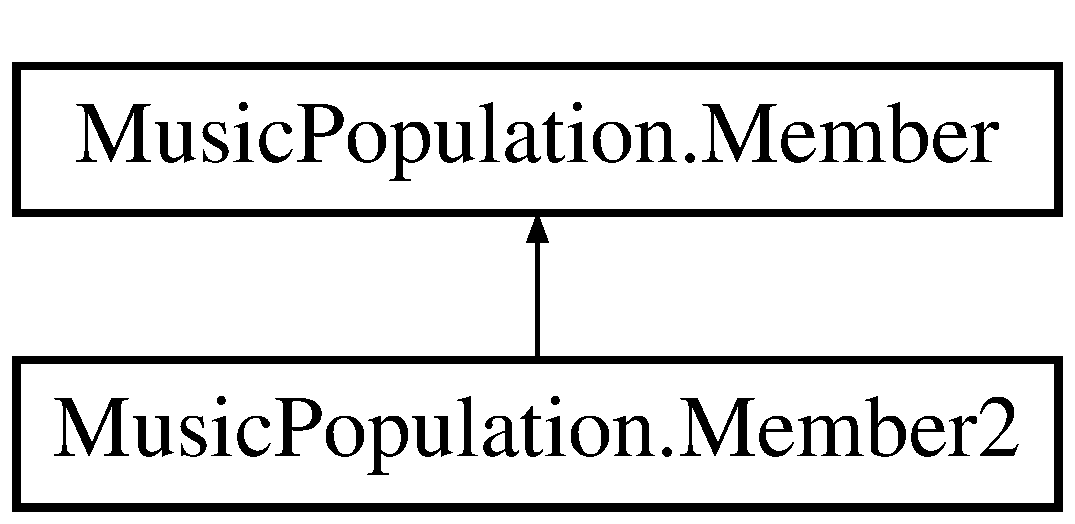
\includegraphics[height=2.000000cm]{class_music_population_1_1_member2}
\end{center}
\end{figure}
\subsection*{Public Member Functions}
\begin{DoxyCompactItemize}
\item 
override int \hyperlink{class_music_population_1_1_member2_a1978ab05a86b98491d5ce7d201cfd4f0}{Rank} ()
\begin{DoxyCompactList}\small\item\em Rank of the member. \end{DoxyCompactList}\item 
override void \hyperlink{class_music_population_1_1_member2_a30e51d2e61399a954b006cdbd6a37952}{Mutate} (Random rand\+Context)
\begin{DoxyCompactList}\small\item\em Method responsible for member mutation. \end{DoxyCompactList}\item 
override void \hyperlink{class_music_population_1_1_member2_af413c7ad74a1979698f87fece3d02f3e}{Influence} (\hyperlink{class_music_population_1_1_member}{Member} influencer, Random rand\+Context)
\begin{DoxyCompactList}\small\item\em Method responible for influencing individual. \end{DoxyCompactList}\item 
\hypertarget{class_music_population_1_1_member2_a77c259e324f669d446ba8c3a4a8e959f}{{\bfseries Member2} (Random rand\+Context)}\label{class_music_population_1_1_member2_a77c259e324f669d446ba8c3a4a8e959f}

\item 
override \hyperlink{class_music_population_1_1_member}{Member} \hyperlink{class_music_population_1_1_member2_a6e676c34e7af1ef9ffbbe68cfa38424f}{Clone} ()
\begin{DoxyCompactList}\small\item\em Clone member. \end{DoxyCompactList}\end{DoxyCompactItemize}
\subsection*{Static Public Attributes}
\begin{DoxyCompactItemize}
\item 
\hypertarget{class_music_population_1_1_member2_acc6a6df1d3a59bfbc5a98079f7380d0a}{static double {\bfseries Pitch\+Influence\+Amount} = 0.\+05}\label{class_music_population_1_1_member2_acc6a6df1d3a59bfbc5a98079f7380d0a}

\item 
\hypertarget{class_music_population_1_1_member2_aa32e3d4e5efd44ffcc61800131879222}{static double {\bfseries Rhythm\+Influence\+Amount} = 0.\+05}\label{class_music_population_1_1_member2_aa32e3d4e5efd44ffcc61800131879222}

\item 
\hypertarget{class_music_population_1_1_member2_a69db93212a8844ddeea740a67f0e3549}{static double {\bfseries Dynamics\+Influence\+Amount} = 0.\+05}\label{class_music_population_1_1_member2_a69db93212a8844ddeea740a67f0e3549}

\item 
\hypertarget{class_music_population_1_1_member2_a0cc907c865be2515d8fefe7daf96eab3}{static double {\bfseries Pause\+Influence\+Amount} = 0.\+05}\label{class_music_population_1_1_member2_a0cc907c865be2515d8fefe7daf96eab3}

\item 
\hypertarget{class_music_population_1_1_member2_a0f6c8ffe0039644b06a0a57f7253a6d4}{static double {\bfseries Rhythm\+Distortion\+Influence\+Chance} = 0.\+05}\label{class_music_population_1_1_member2_a0f6c8ffe0039644b06a0a57f7253a6d4}

\item 
\hypertarget{class_music_population_1_1_member2_a3fe5b6a8392f753bb7e39aaa21f219fd}{static double {\bfseries Dynamics\+Distortion\+Influence\+Chance} = 0.\+05}\label{class_music_population_1_1_member2_a3fe5b6a8392f753bb7e39aaa21f219fd}

\item 
\hypertarget{class_music_population_1_1_member2_ab9ca3b61729112b343104e154150b82d}{static double {\bfseries Type\+Influence\+Chance} = 0.\+2}\label{class_music_population_1_1_member2_ab9ca3b61729112b343104e154150b82d}

\item 
\hypertarget{class_music_population_1_1_member2_ab889e8c8c0bbce32ec788ded5a98fbdf}{static double {\bfseries Growth\+Chance} = 0.\+5}\label{class_music_population_1_1_member2_ab889e8c8c0bbce32ec788ded5a98fbdf}

\item 
\hypertarget{class_music_population_1_1_member2_acdaaab2cd3eebbd202ce7e8192c85cec}{static double {\bfseries Shrink\+Chance} = 0.\+05}\label{class_music_population_1_1_member2_acdaaab2cd3eebbd202ce7e8192c85cec}

\item 
\hypertarget{class_music_population_1_1_member2_a525b83ae02f295f6c74a809169d1a9b1}{static double {\bfseries Peak\+Move\+Chance} = 0.\+05}\label{class_music_population_1_1_member2_a525b83ae02f295f6c74a809169d1a9b1}

\item 
\hypertarget{class_music_population_1_1_member2_a9d485a62f262793819fb6b510958b153}{static int {\bfseries Peak\+Max\+Move} = 7}\label{class_music_population_1_1_member2_a9d485a62f262793819fb6b510958b153}

\item 
\hypertarget{class_music_population_1_1_member2_a377f9971e60116719b4ace739a491bc9}{static double {\bfseries Pause\+Change\+Chance} = 0.\+05}\label{class_music_population_1_1_member2_a377f9971e60116719b4ace739a491bc9}

\item 
\hypertarget{class_music_population_1_1_member2_ad135a25f8421b7ee086d7b8f65ec037e}{static int {\bfseries Pause\+Max\+Change} = 20}\label{class_music_population_1_1_member2_ad135a25f8421b7ee086d7b8f65ec037e}

\item 
\hypertarget{class_music_population_1_1_member2_a56aa903e1ec052ffa2f4919d3fea8b79}{static double {\bfseries Initial\+Rhythm\+Change\+Chance} = 0.\+05}\label{class_music_population_1_1_member2_a56aa903e1ec052ffa2f4919d3fea8b79}

\item 
\hypertarget{class_music_population_1_1_member2_a707e52a9a4c1913b95d0cad061558f27}{static int {\bfseries Initial\+Rhythm\+Max\+Change} = 7}\label{class_music_population_1_1_member2_a707e52a9a4c1913b95d0cad061558f27}

\item 
\hypertarget{class_music_population_1_1_member2_a4efdd9b8c8fef2aebab9b83a7c8be2c5}{static double {\bfseries Initial\+Dynamics\+Change\+Chance} = 0.\+05}\label{class_music_population_1_1_member2_a4efdd9b8c8fef2aebab9b83a7c8be2c5}

\item 
\hypertarget{class_music_population_1_1_member2_a0e7cbcf6bc3b08e78849d4403a2d5901}{static int {\bfseries Initial\+Dynamics\+Max\+Change} = 20}\label{class_music_population_1_1_member2_a0e7cbcf6bc3b08e78849d4403a2d5901}

\item 
\hypertarget{class_music_population_1_1_member2_a79fa86aa7fff7365e733e5daa686160e}{static double {\bfseries Initial\+Chord\+Change\+Chance} = 0.\+05}\label{class_music_population_1_1_member2_a79fa86aa7fff7365e733e5daa686160e}

\item 
\hypertarget{class_music_population_1_1_member2_ae639e3e64ace1dd711c6410ff8fbd9a5}{static double {\bfseries Chord\+Change\+Chance} = 0.\+05}\label{class_music_population_1_1_member2_ae639e3e64ace1dd711c6410ff8fbd9a5}

\item 
\hypertarget{class_music_population_1_1_member2_a854810e0c221d5d52b3b367f1b79ff18}{static double {\bfseries Rhythm\+Distortion\+Change\+Chance} = 0.\+05}\label{class_music_population_1_1_member2_a854810e0c221d5d52b3b367f1b79ff18}

\item 
\hypertarget{class_music_population_1_1_member2_a96ffb908162ce83169c0a5ef43407b28}{static double {\bfseries Dynamics\+Distortion\+Change\+Chance} = 0.\+05}\label{class_music_population_1_1_member2_a96ffb908162ce83169c0a5ef43407b28}

\item 
\hypertarget{class_music_population_1_1_member2_a63c9f376d6b094a2535d83a56c4d3030}{static double {\bfseries Pitch\+Change\+Chance} = 0.\+05}\label{class_music_population_1_1_member2_a63c9f376d6b094a2535d83a56c4d3030}

\item 
\hypertarget{class_music_population_1_1_member2_a0c82bcef65296b921d0be3e5b3fc8f57}{static int {\bfseries Pitch\+Max\+Change} = 5}\label{class_music_population_1_1_member2_a0c82bcef65296b921d0be3e5b3fc8f57}

\item 
\hypertarget{class_music_population_1_1_member2_aedd0c5f9c974c64f7935138be1761d8f}{static double {\bfseries Rhythm\+Change\+Chance} = 0.\+05}\label{class_music_population_1_1_member2_aedd0c5f9c974c64f7935138be1761d8f}

\item 
\hypertarget{class_music_population_1_1_member2_ac04a8e31cd3167d763b6ff76c09ff7e3}{static int {\bfseries Rhythm\+Max\+Change} = 5}\label{class_music_population_1_1_member2_ac04a8e31cd3167d763b6ff76c09ff7e3}

\item 
\hypertarget{class_music_population_1_1_member2_a4405fd9bdf51d621768ebc3585c4f601}{static double {\bfseries Dynamics\+Change\+Chance} = 0.\+05}\label{class_music_population_1_1_member2_a4405fd9bdf51d621768ebc3585c4f601}

\item 
\hypertarget{class_music_population_1_1_member2_ab87cfb3d5ff661c6a18aa8e79d41c20e}{static int {\bfseries Dynamics\+Max\+Change} = 20}\label{class_music_population_1_1_member2_ab87cfb3d5ff661c6a18aa8e79d41c20e}

\item 
\hypertarget{class_music_population_1_1_member2_a73edca70ed1d84402130a22bb2161970}{static int {\bfseries Preffered\+Length} = 25}\label{class_music_population_1_1_member2_a73edca70ed1d84402130a22bb2161970}

\item 
\hypertarget{class_music_population_1_1_member2_a85f949dc40d734b10de8c6bd5e64ecb7}{static int {\bfseries Preffered\+Pause\+Length} = 12}\label{class_music_population_1_1_member2_a85f949dc40d734b10de8c6bd5e64ecb7}

\item 
\hypertarget{class_music_population_1_1_member2_ab57206a0fe05c538448f8c1f39807ee8}{static double {\bfseries Type\+Change\+Chance} = 0.\+1}\label{class_music_population_1_1_member2_ab57206a0fe05c538448f8c1f39807ee8}

\end{DoxyCompactItemize}
\subsection*{Protected Member Functions}
\begin{DoxyCompactItemize}
\item 
\hypertarget{class_music_population_1_1_member2_abae4582df340f8a7906b50fdcff5a445}{void {\bfseries Shrink} ()}\label{class_music_population_1_1_member2_abae4582df340f8a7906b50fdcff5a445}

\item 
\hypertarget{class_music_population_1_1_member2_ae5b7fc755e529b2a03c8e60996ea782e}{void {\bfseries Grow} (Random rand\+Context)}\label{class_music_population_1_1_member2_ae5b7fc755e529b2a03c8e60996ea782e}

\end{DoxyCompactItemize}
\subsection*{Properties}
\begin{DoxyCompactItemize}
\item 
\hypertarget{class_music_population_1_1_member2_a1c0d24f13a1add473466eee243f54b30}{override int {\bfseries Number\+Of\+Notes}\hspace{0.3cm}{\ttfamily  \mbox{[}get\mbox{]}}}\label{class_music_population_1_1_member2_a1c0d24f13a1add473466eee243f54b30}

\item 
\hypertarget{class_music_population_1_1_member2_ae73d7137c58d2f40c8f5849c836af4c1}{override int\mbox{[},\mbox{]} {\bfseries Notes}\hspace{0.3cm}{\ttfamily  \mbox{[}get\mbox{]}}}\label{class_music_population_1_1_member2_ae73d7137c58d2f40c8f5849c836af4c1}

\end{DoxyCompactItemize}
\subsection*{Additional Inherited Members}


\subsection{Detailed Description}
Implementation of second phase member. 



\subsection{Member Function Documentation}
\hypertarget{class_music_population_1_1_member2_a6e676c34e7af1ef9ffbbe68cfa38424f}{\index{Music\+Population\+::\+Member2@{Music\+Population\+::\+Member2}!Clone@{Clone}}
\index{Clone@{Clone}!Music\+Population\+::\+Member2@{Music\+Population\+::\+Member2}}
\subsubsection[{Clone}]{\setlength{\rightskip}{0pt plus 5cm}override {\bf Member} Music\+Population.\+Member2.\+Clone (
\begin{DoxyParamCaption}
{}
\end{DoxyParamCaption}
)\hspace{0.3cm}{\ttfamily [virtual]}}}\label{class_music_population_1_1_member2_a6e676c34e7af1ef9ffbbe68cfa38424f}


Clone member. 

\begin{DoxyReturn}{Returns}
copy of member
\end{DoxyReturn}


Implements \hyperlink{class_music_population_1_1_member_af310ebdf342531da3edc882987574a16}{Music\+Population.\+Member}.

\hypertarget{class_music_population_1_1_member2_af413c7ad74a1979698f87fece3d02f3e}{\index{Music\+Population\+::\+Member2@{Music\+Population\+::\+Member2}!Influence@{Influence}}
\index{Influence@{Influence}!Music\+Population\+::\+Member2@{Music\+Population\+::\+Member2}}
\subsubsection[{Influence}]{\setlength{\rightskip}{0pt plus 5cm}override void Music\+Population.\+Member2.\+Influence (
\begin{DoxyParamCaption}
\item[{{\bf Member}}]{influencer, }
\item[{Random}]{rand\+Context}
\end{DoxyParamCaption}
)\hspace{0.3cm}{\ttfamily [virtual]}}}\label{class_music_population_1_1_member2_af413c7ad74a1979698f87fece3d02f3e}


Method responible for influencing individual. 


\begin{DoxyParams}{Parameters}
{\em influencer} & \hyperlink{class_music_population_1_1_member}{Member} which should be influenced\\
\hline
{\em rand\+Context} & random context\\
\hline
\end{DoxyParams}


Implements \hyperlink{class_music_population_1_1_member_a99042d0181ef0e48ad71d45313a176b6}{Music\+Population.\+Member}.

\hypertarget{class_music_population_1_1_member2_a30e51d2e61399a954b006cdbd6a37952}{\index{Music\+Population\+::\+Member2@{Music\+Population\+::\+Member2}!Mutate@{Mutate}}
\index{Mutate@{Mutate}!Music\+Population\+::\+Member2@{Music\+Population\+::\+Member2}}
\subsubsection[{Mutate}]{\setlength{\rightskip}{0pt plus 5cm}override void Music\+Population.\+Member2.\+Mutate (
\begin{DoxyParamCaption}
\item[{Random}]{rand\+Context}
\end{DoxyParamCaption}
)\hspace{0.3cm}{\ttfamily [virtual]}}}\label{class_music_population_1_1_member2_a30e51d2e61399a954b006cdbd6a37952}


Method responsible for member mutation. 


\begin{DoxyParams}{Parameters}
{\em rand\+Context} & random context\\
\hline
\end{DoxyParams}


Implements \hyperlink{class_music_population_1_1_member_affe5eeed6ac4b042d5729991f0c39eba}{Music\+Population.\+Member}.

\hypertarget{class_music_population_1_1_member2_a1978ab05a86b98491d5ce7d201cfd4f0}{\index{Music\+Population\+::\+Member2@{Music\+Population\+::\+Member2}!Rank@{Rank}}
\index{Rank@{Rank}!Music\+Population\+::\+Member2@{Music\+Population\+::\+Member2}}
\subsubsection[{Rank}]{\setlength{\rightskip}{0pt plus 5cm}override int Music\+Population.\+Member2.\+Rank (
\begin{DoxyParamCaption}
{}
\end{DoxyParamCaption}
)\hspace{0.3cm}{\ttfamily [virtual]}}}\label{class_music_population_1_1_member2_a1978ab05a86b98491d5ce7d201cfd4f0}


Rank of the member. 

\begin{DoxyReturn}{Returns}
integer representing rank of member
\end{DoxyReturn}


Implements \hyperlink{class_music_population_1_1_member_a238549ad669c4f8eda036e608beba422}{Music\+Population.\+Member}.



The documentation for this class was generated from the following files\+:\begin{DoxyCompactItemize}
\item 
C\+:/\+Users/praktykant/\+Documents/\+Git\+Hub/\+Harmony-\/\+Simulation/\+Populo/\+Music\+Population/\+Components/\+Member/Member2.\+cs\item 
C\+:/\+Users/praktykant/\+Documents/\+Git\+Hub/\+Harmony-\/\+Simulation/\+Populo/\+Music\+Population/\+Components/\+Member/Member2\+Parameters.\+cs\end{DoxyCompactItemize}

\hypertarget{class_music_population_1_1_member3}{\section{Music\+Population.\+Member3 Class Reference}
\label{class_music_population_1_1_member3}\index{Music\+Population.\+Member3@{Music\+Population.\+Member3}}
}


Implementation of third phase member.  


Inheritance diagram for Music\+Population.\+Member3\+:\begin{figure}[H]
\begin{center}
\leavevmode
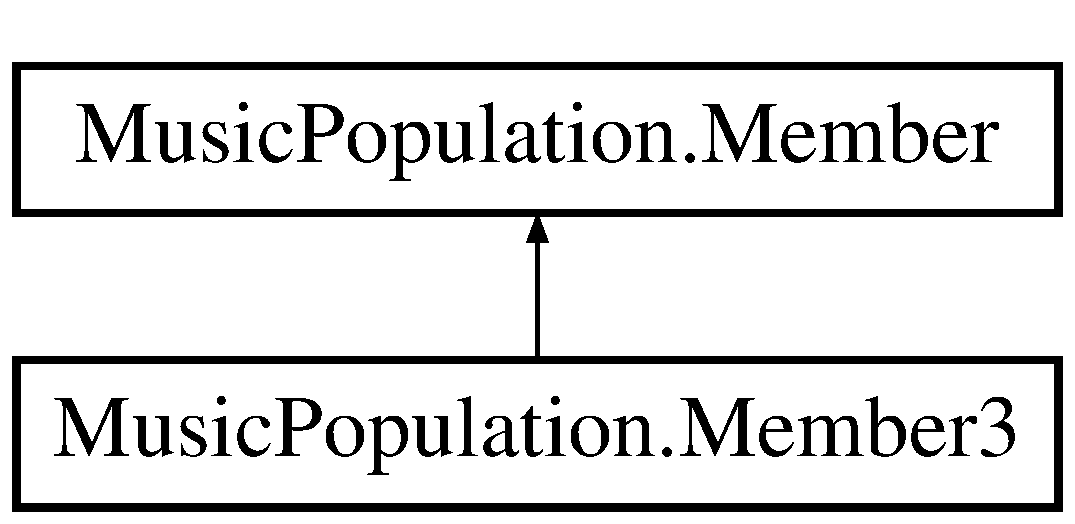
\includegraphics[height=2.000000cm]{class_music_population_1_1_member3}
\end{center}
\end{figure}
\subsection*{Public Member Functions}
\begin{DoxyCompactItemize}
\item 
override int \hyperlink{class_music_population_1_1_member3_a3148bb13399637bb2cf2addf6d8ecbec}{Rank} ()
\begin{DoxyCompactList}\small\item\em Rank of the member. \end{DoxyCompactList}\item 
override void \hyperlink{class_music_population_1_1_member3_a443d06792b6e3566308a67d56e31c2d8}{Mutate} (Random rand\+Context)
\begin{DoxyCompactList}\small\item\em Method responsible for member mutation. \end{DoxyCompactList}\item 
override void \hyperlink{class_music_population_1_1_member3_aabde212fac4cd75573a3ed07b6522e1d}{Influence} (\hyperlink{class_music_population_1_1_member}{Member} influencer, Random rand\+Context)
\begin{DoxyCompactList}\small\item\em Method responible for influencing individual. \end{DoxyCompactList}\item 
override \hyperlink{class_music_population_1_1_member}{Member} \hyperlink{class_music_population_1_1_member3_ae37f77498a7c3ccec6b8531746eff1ec}{Clone} ()
\begin{DoxyCompactList}\small\item\em Clone member. \end{DoxyCompactList}\item 
\hypertarget{class_music_population_1_1_member3_a64e08c71b9df2f480a2f71325bb45058}{{\bfseries Member3} (Random rand\+Context)}\label{class_music_population_1_1_member3_a64e08c71b9df2f480a2f71325bb45058}

\end{DoxyCompactItemize}
\subsection*{Static Public Attributes}
\begin{DoxyCompactItemize}
\item 
\hypertarget{class_music_population_1_1_member3_a0f2432f6350e143c9481a396aa772488}{static int\mbox{[}$\,$\mbox{]} {\bfseries Modify\+Amount} = new int\mbox{[}$\,$\mbox{]} \{ 3, 2, 5, 3, 15, 3,2 \}}\label{class_music_population_1_1_member3_a0f2432f6350e143c9481a396aa772488}

\item 
\hypertarget{class_music_population_1_1_member3_a1c5540a52ddaf4bf79860228ec2d0c6d}{static double\mbox{[}$\,$\mbox{]} {\bfseries Influence\+Amount} = new double\mbox{[}$\,$\mbox{]} \{ 0.\+2, 0.\+2, 0.\+2, 0.\+2, 0.\+2, 0.\+2,0 \}}\label{class_music_population_1_1_member3_a1c5540a52ddaf4bf79860228ec2d0c6d}

\item 
\hypertarget{class_music_population_1_1_member3_aee4d992f98eae4b1041d23d3e16dbf25}{static double\mbox{[}$\,$\mbox{]} {\bfseries Transpose\+Chance} = new double\mbox{[}$\,$\mbox{]} \{ 0.\+05, 0.\+05, 0.\+05, 0.\+05, 0.\+05, 0.\+05, 0.\+05 \}}\label{class_music_population_1_1_member3_aee4d992f98eae4b1041d23d3e16dbf25}

\item 
\hypertarget{class_music_population_1_1_member3_ad1e54d4ec4deb35b63ea19d99781a933}{static double\mbox{[}$\,$\mbox{]} {\bfseries Exchange\+Chance} = new double\mbox{[}$\,$\mbox{]} \{ 0.\+05, 0.\+05, 0.\+05, 0.\+05, 0.\+05, 0.\+05, 0.\+05 \}}\label{class_music_population_1_1_member3_ad1e54d4ec4deb35b63ea19d99781a933}

\item 
\hypertarget{class_music_population_1_1_member3_aeef13e2b79c4d030a44f9668beaa4e94}{static double\mbox{[}$\,$\mbox{]} {\bfseries Modify\+Chance} = new double\mbox{[}$\,$\mbox{]} \{ 0.\+05, 0.\+05, 0.\+05, 0.\+05, 0.\+05, 0.\+05, 0.\+05 \}}\label{class_music_population_1_1_member3_aeef13e2b79c4d030a44f9668beaa4e94}

\item 
\hypertarget{class_music_population_1_1_member3_aeab9c6bd36d28028d98abcd9164907b8}{static double {\bfseries Growth\+Chance} = 0.\+05}\label{class_music_population_1_1_member3_aeab9c6bd36d28028d98abcd9164907b8}

\item 
\hypertarget{class_music_population_1_1_member3_a0e5ce99e51dfbbb45aa8772bfc213a13}{static double {\bfseries Shrink\+Chance} = 0.\+05}\label{class_music_population_1_1_member3_a0e5ce99e51dfbbb45aa8772bfc213a13}

\item 
\hypertarget{class_music_population_1_1_member3_a930d4be917d694eaa957ba4989fe7c23}{static int {\bfseries Preffered\+Length} = 300}\label{class_music_population_1_1_member3_a930d4be917d694eaa957ba4989fe7c23}

\item 
\hypertarget{class_music_population_1_1_member3_a3dfb4ff64667f49ab80db4926d38d0d2}{static int {\bfseries Preffered\+Groups} =10}\label{class_music_population_1_1_member3_a3dfb4ff64667f49ab80db4926d38d0d2}

\item 
\hypertarget{class_music_population_1_1_member3_a0151620624164750c4f3f8a06a490586}{static int {\bfseries Preffered\+Notes} = 50}\label{class_music_population_1_1_member3_a0151620624164750c4f3f8a06a490586}

\item 
\hypertarget{class_music_population_1_1_member3_a25ef5c37a1e77339811361dbf40bb0ea}{static int {\bfseries Played\+Group} = 0}\label{class_music_population_1_1_member3_a25ef5c37a1e77339811361dbf40bb0ea}

\end{DoxyCompactItemize}
\subsection*{Protected Member Functions}
\begin{DoxyCompactItemize}
\item 
\hypertarget{class_music_population_1_1_member3_ae9ba132fdb49dbdd756d66b286cb164d}{void {\bfseries Transpose} (uint n, Random rand\+Context)}\label{class_music_population_1_1_member3_ae9ba132fdb49dbdd756d66b286cb164d}

\item 
\hypertarget{class_music_population_1_1_member3_aa081ffe848adf82a4fd2a683b9adb9ea}{void {\bfseries Exchange} (uint n, Random rand\+Context)}\label{class_music_population_1_1_member3_aa081ffe848adf82a4fd2a683b9adb9ea}

\item 
\hypertarget{class_music_population_1_1_member3_a1ae8fde6d20043b2d9e06c7ebb6b08ca}{void {\bfseries Modify} (uint n, Random rand\+Context)}\label{class_music_population_1_1_member3_a1ae8fde6d20043b2d9e06c7ebb6b08ca}

\item 
\hypertarget{class_music_population_1_1_member3_a7b27b07ab3c2ffc20e06d9fae9182dcc}{void {\bfseries Shrink} ()}\label{class_music_population_1_1_member3_a7b27b07ab3c2ffc20e06d9fae9182dcc}

\item 
\hypertarget{class_music_population_1_1_member3_a0e2fd531ab8add6f8b8b737a60bbb006}{void {\bfseries Grow} (Random rand\+Context)}\label{class_music_population_1_1_member3_a0e2fd531ab8add6f8b8b737a60bbb006}

\end{DoxyCompactItemize}
\subsection*{Properties}
\begin{DoxyCompactItemize}
\item 
\hypertarget{class_music_population_1_1_member3_a3a02315e983d81c72581dd9d39b6af52}{override int {\bfseries Number\+Of\+Notes}\hspace{0.3cm}{\ttfamily  \mbox{[}get\mbox{]}}}\label{class_music_population_1_1_member3_a3a02315e983d81c72581dd9d39b6af52}

\item 
\hypertarget{class_music_population_1_1_member3_a277a89aa1335d01b38edd8cd78ca1add}{override int\mbox{[},\mbox{]} {\bfseries Notes}\hspace{0.3cm}{\ttfamily  \mbox{[}get\mbox{]}}}\label{class_music_population_1_1_member3_a277a89aa1335d01b38edd8cd78ca1add}

\end{DoxyCompactItemize}
\subsection*{Additional Inherited Members}


\subsection{Detailed Description}
Implementation of third phase member. 



\subsection{Member Function Documentation}
\hypertarget{class_music_population_1_1_member3_ae37f77498a7c3ccec6b8531746eff1ec}{\index{Music\+Population\+::\+Member3@{Music\+Population\+::\+Member3}!Clone@{Clone}}
\index{Clone@{Clone}!Music\+Population\+::\+Member3@{Music\+Population\+::\+Member3}}
\subsubsection[{Clone}]{\setlength{\rightskip}{0pt plus 5cm}override {\bf Member} Music\+Population.\+Member3.\+Clone (
\begin{DoxyParamCaption}
{}
\end{DoxyParamCaption}
)\hspace{0.3cm}{\ttfamily [virtual]}}}\label{class_music_population_1_1_member3_ae37f77498a7c3ccec6b8531746eff1ec}


Clone member. 

\begin{DoxyReturn}{Returns}
copy of member
\end{DoxyReturn}


Implements \hyperlink{class_music_population_1_1_member_af310ebdf342531da3edc882987574a16}{Music\+Population.\+Member}.

\hypertarget{class_music_population_1_1_member3_aabde212fac4cd75573a3ed07b6522e1d}{\index{Music\+Population\+::\+Member3@{Music\+Population\+::\+Member3}!Influence@{Influence}}
\index{Influence@{Influence}!Music\+Population\+::\+Member3@{Music\+Population\+::\+Member3}}
\subsubsection[{Influence}]{\setlength{\rightskip}{0pt plus 5cm}override void Music\+Population.\+Member3.\+Influence (
\begin{DoxyParamCaption}
\item[{{\bf Member}}]{influencer, }
\item[{Random}]{rand\+Context}
\end{DoxyParamCaption}
)\hspace{0.3cm}{\ttfamily [virtual]}}}\label{class_music_population_1_1_member3_aabde212fac4cd75573a3ed07b6522e1d}


Method responible for influencing individual. 


\begin{DoxyParams}{Parameters}
{\em influencer} & \hyperlink{class_music_population_1_1_member}{Member} which should be influenced\\
\hline
{\em rand\+Context} & random context\\
\hline
\end{DoxyParams}


Implements \hyperlink{class_music_population_1_1_member_a99042d0181ef0e48ad71d45313a176b6}{Music\+Population.\+Member}.

\hypertarget{class_music_population_1_1_member3_a443d06792b6e3566308a67d56e31c2d8}{\index{Music\+Population\+::\+Member3@{Music\+Population\+::\+Member3}!Mutate@{Mutate}}
\index{Mutate@{Mutate}!Music\+Population\+::\+Member3@{Music\+Population\+::\+Member3}}
\subsubsection[{Mutate}]{\setlength{\rightskip}{0pt plus 5cm}override void Music\+Population.\+Member3.\+Mutate (
\begin{DoxyParamCaption}
\item[{Random}]{rand\+Context}
\end{DoxyParamCaption}
)\hspace{0.3cm}{\ttfamily [virtual]}}}\label{class_music_population_1_1_member3_a443d06792b6e3566308a67d56e31c2d8}


Method responsible for member mutation. 


\begin{DoxyParams}{Parameters}
{\em rand\+Context} & random context\\
\hline
\end{DoxyParams}


Implements \hyperlink{class_music_population_1_1_member_affe5eeed6ac4b042d5729991f0c39eba}{Music\+Population.\+Member}.

\hypertarget{class_music_population_1_1_member3_a3148bb13399637bb2cf2addf6d8ecbec}{\index{Music\+Population\+::\+Member3@{Music\+Population\+::\+Member3}!Rank@{Rank}}
\index{Rank@{Rank}!Music\+Population\+::\+Member3@{Music\+Population\+::\+Member3}}
\subsubsection[{Rank}]{\setlength{\rightskip}{0pt plus 5cm}override int Music\+Population.\+Member3.\+Rank (
\begin{DoxyParamCaption}
{}
\end{DoxyParamCaption}
)\hspace{0.3cm}{\ttfamily [virtual]}}}\label{class_music_population_1_1_member3_a3148bb13399637bb2cf2addf6d8ecbec}


Rank of the member. 

\begin{DoxyReturn}{Returns}
integer representing rank of member
\end{DoxyReturn}


Implements \hyperlink{class_music_population_1_1_member_a238549ad669c4f8eda036e608beba422}{Music\+Population.\+Member}.



The documentation for this class was generated from the following files\+:\begin{DoxyCompactItemize}
\item 
C\+:/\+Users/praktykant/\+Documents/\+Git\+Hub/\+Harmony-\/\+Simulation/\+Populo/\+Music\+Population/\+Components/\+Member/Member3.\+cs\item 
C\+:/\+Users/praktykant/\+Documents/\+Git\+Hub/\+Harmony-\/\+Simulation/\+Populo/\+Music\+Population/\+Components/\+Member/Member3\+Parameters.\+cs\end{DoxyCompactItemize}

\hypertarget{class_periodic_chords_1_1_midi_cent_periodic_chord}{\section{Periodic\+Chords.\+Midi\+Cent\+Periodic\+Chord Class Reference}
\label{class_periodic_chords_1_1_midi_cent_periodic_chord}\index{Periodic\+Chords.\+Midi\+Cent\+Periodic\+Chord@{Periodic\+Chords.\+Midi\+Cent\+Periodic\+Chord}}
}
Inheritance diagram for Periodic\+Chords.\+Midi\+Cent\+Periodic\+Chord\+:\begin{figure}[H]
\begin{center}
\leavevmode
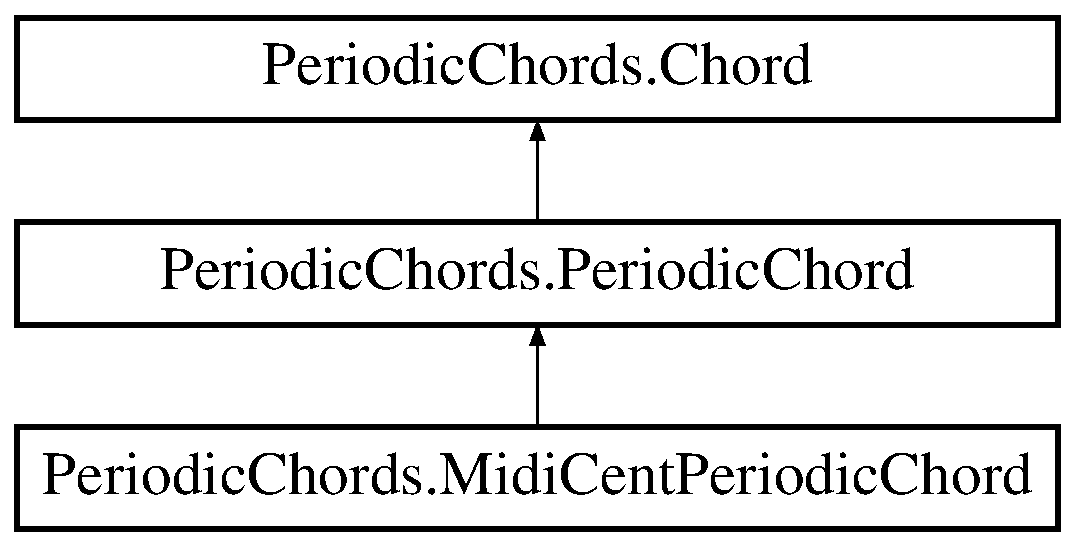
\includegraphics[height=3.000000cm]{class_periodic_chords_1_1_midi_cent_periodic_chord}
\end{center}
\end{figure}
\subsection*{Properties}
\begin{DoxyCompactItemize}
\item 
\hypertarget{class_periodic_chords_1_1_midi_cent_periodic_chord_a53fb6447477b22579280d5ded1b2daf2}{override double\mbox{[}$\,$\mbox{]} {\bfseries Frequencies}\hspace{0.3cm}{\ttfamily  \mbox{[}get\mbox{]}}}\label{class_periodic_chords_1_1_midi_cent_periodic_chord_a53fb6447477b22579280d5ded1b2daf2}

\item 
\hypertarget{class_periodic_chords_1_1_midi_cent_periodic_chord_acd8d30256b212e5e8048a147554f34b3}{override double\mbox{[}$\,$\mbox{]} {\bfseries Notes}\hspace{0.3cm}{\ttfamily  \mbox{[}get\mbox{]}}}\label{class_periodic_chords_1_1_midi_cent_periodic_chord_acd8d30256b212e5e8048a147554f34b3}

\end{DoxyCompactItemize}
\subsection*{Additional Inherited Members}


The documentation for this class was generated from the following file\+:\begin{DoxyCompactItemize}
\item 
C\+:/\+Users/praktykant/\+Documents/\+Git\+Hub/\+Harmony-\/\+Simulation/\+Harmony\+Editor/\+Periodic\+Chords/Periodic\+Chord.\+cs\end{DoxyCompactItemize}

\hypertarget{class_periodic_chords_1_1_midi_cent_simple_chord}{\section{Periodic\+Chords.\+Midi\+Cent\+Simple\+Chord Class Reference}
\label{class_periodic_chords_1_1_midi_cent_simple_chord}\index{Periodic\+Chords.\+Midi\+Cent\+Simple\+Chord@{Periodic\+Chords.\+Midi\+Cent\+Simple\+Chord}}
}
Inheritance diagram for Periodic\+Chords.\+Midi\+Cent\+Simple\+Chord\+:\begin{figure}[H]
\begin{center}
\leavevmode
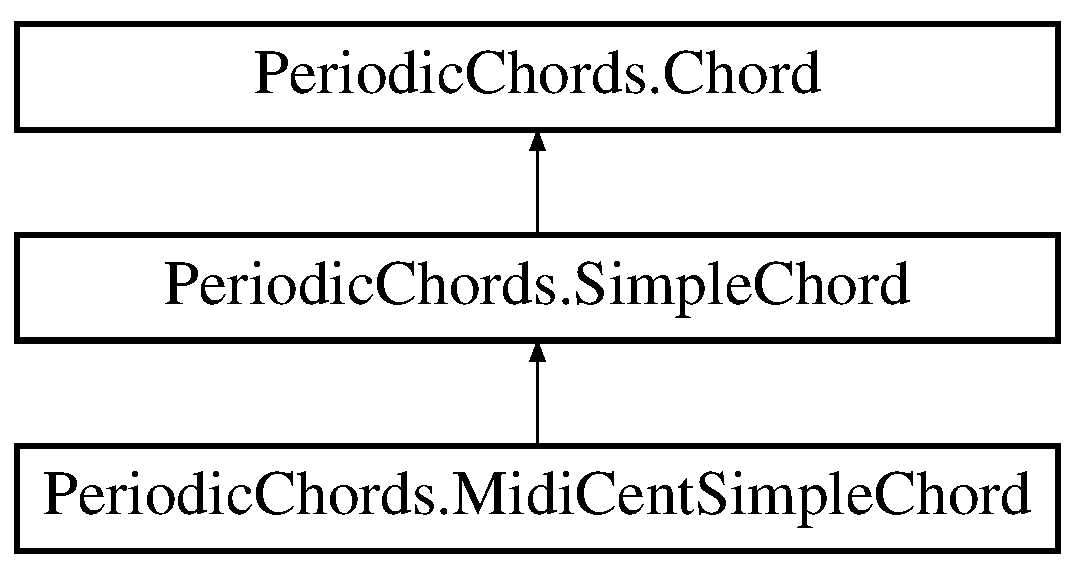
\includegraphics[height=3.000000cm]{class_periodic_chords_1_1_midi_cent_simple_chord}
\end{center}
\end{figure}
\subsection*{Properties}
\begin{DoxyCompactItemize}
\item 
\hypertarget{class_periodic_chords_1_1_midi_cent_simple_chord_a717c9bbbd90aea19cf949b02bbe6f1d5}{override double\mbox{[}$\,$\mbox{]} {\bfseries Frequencies}\hspace{0.3cm}{\ttfamily  \mbox{[}get\mbox{]}}}\label{class_periodic_chords_1_1_midi_cent_simple_chord_a717c9bbbd90aea19cf949b02bbe6f1d5}

\item 
\hypertarget{class_periodic_chords_1_1_midi_cent_simple_chord_a6e61b7c207ec293d2f72846550ddf879}{override double\mbox{[}$\,$\mbox{]} {\bfseries Notes}\hspace{0.3cm}{\ttfamily  \mbox{[}get\mbox{]}}}\label{class_periodic_chords_1_1_midi_cent_simple_chord_a6e61b7c207ec293d2f72846550ddf879}

\end{DoxyCompactItemize}
\subsection*{Additional Inherited Members}


The documentation for this class was generated from the following file\+:\begin{DoxyCompactItemize}
\item 
C\+:/\+Users/praktykant/\+Documents/\+Git\+Hub/\+Harmony-\/\+Simulation/\+Harmony\+Editor/\+Periodic\+Chords/Simple\+Chord.\+cs\end{DoxyCompactItemize}

\hypertarget{class_periodic_chords_1_1_midi_periodic_chord}{\section{Periodic\+Chords.\+Midi\+Periodic\+Chord Class Reference}
\label{class_periodic_chords_1_1_midi_periodic_chord}\index{Periodic\+Chords.\+Midi\+Periodic\+Chord@{Periodic\+Chords.\+Midi\+Periodic\+Chord}}
}
Inheritance diagram for Periodic\+Chords.\+Midi\+Periodic\+Chord\+:\begin{figure}[H]
\begin{center}
\leavevmode
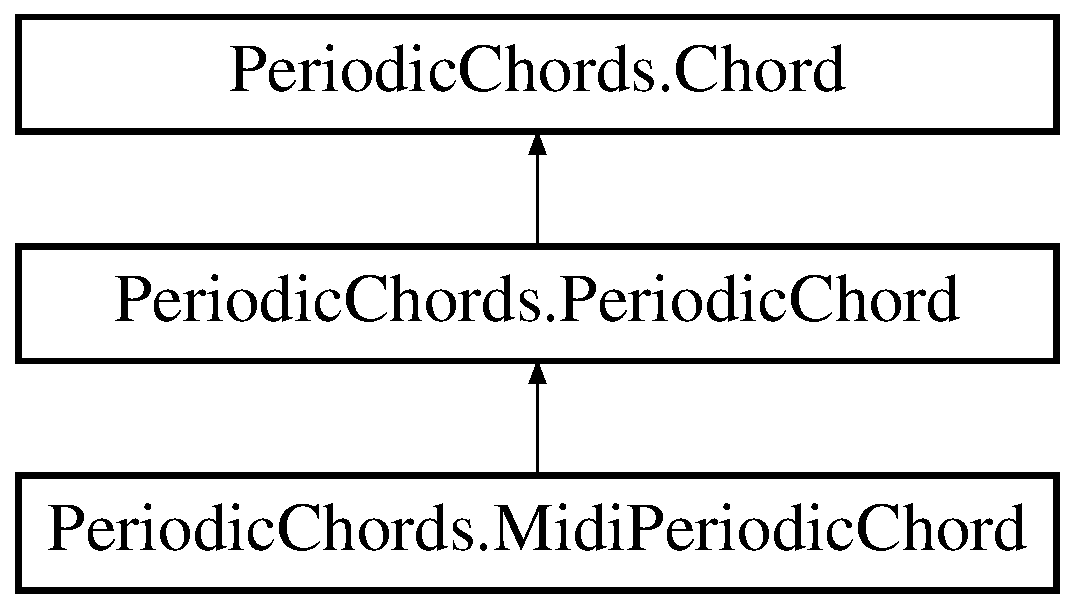
\includegraphics[height=3.000000cm]{class_periodic_chords_1_1_midi_periodic_chord}
\end{center}
\end{figure}
\subsection*{Properties}
\begin{DoxyCompactItemize}
\item 
\hypertarget{class_periodic_chords_1_1_midi_periodic_chord_a53e10613924317f1d3fc92def7b62cab}{override double\mbox{[}$\,$\mbox{]} {\bfseries Frequencies}\hspace{0.3cm}{\ttfamily  \mbox{[}get\mbox{]}}}\label{class_periodic_chords_1_1_midi_periodic_chord_a53e10613924317f1d3fc92def7b62cab}

\item 
\hypertarget{class_periodic_chords_1_1_midi_periodic_chord_a23ec201aea969c6a95638f0cc2cc0f73}{override double\mbox{[}$\,$\mbox{]} {\bfseries Notes}\hspace{0.3cm}{\ttfamily  \mbox{[}get\mbox{]}}}\label{class_periodic_chords_1_1_midi_periodic_chord_a23ec201aea969c6a95638f0cc2cc0f73}

\end{DoxyCompactItemize}
\subsection*{Additional Inherited Members}


The documentation for this class was generated from the following file\+:\begin{DoxyCompactItemize}
\item 
C\+:/\+Users/praktykant/\+Documents/\+Git\+Hub/\+Harmony-\/\+Simulation/\+Harmony\+Editor/\+Periodic\+Chords/Periodic\+Chord.\+cs\end{DoxyCompactItemize}

\hypertarget{class_populo_application_1_1_m_i_d_i_player}{\section{Populo\+Application.\+M\+I\+D\+I\+Player Class Reference}
\label{class_populo_application_1_1_m_i_d_i_player}\index{Populo\+Application.\+M\+I\+D\+I\+Player@{Populo\+Application.\+M\+I\+D\+I\+Player}}
}
\subsection*{Public Member Functions}
\begin{DoxyCompactItemize}
\item 
\hypertarget{class_populo_application_1_1_m_i_d_i_player_a0823f764c3cbfd3627b60d2c108056a2}{{\bfseries M\+I\+D\+I\+Player} (int device, int number\+Of\+Tracks, int interval)}\label{class_populo_application_1_1_m_i_d_i_player_a0823f764c3cbfd3627b60d2c108056a2}

\item 
\hypertarget{class_populo_application_1_1_m_i_d_i_player_a505b4bfce27dc991d04431a840c9df4d}{void {\bfseries Start} ()}\label{class_populo_application_1_1_m_i_d_i_player_a505b4bfce27dc991d04431a840c9df4d}

\item 
\hypertarget{class_populo_application_1_1_m_i_d_i_player_a77c3144d6d8900541b3ea2b3a3d7d24b}{void {\bfseries Pause} ()}\label{class_populo_application_1_1_m_i_d_i_player_a77c3144d6d8900541b3ea2b3a3d7d24b}

\item 
\hypertarget{class_populo_application_1_1_m_i_d_i_player_a467a3c2662628f43e2a4da5ad1fdcc1e}{void {\bfseries Stop} ()}\label{class_populo_application_1_1_m_i_d_i_player_a467a3c2662628f43e2a4da5ad1fdcc1e}

\item 
\hypertarget{class_populo_application_1_1_m_i_d_i_player_a273e31c34b35bb0358f1f02082a55888}{void {\bfseries Tick} (object sender, Elapsed\+Event\+Args e)}\label{class_populo_application_1_1_m_i_d_i_player_a273e31c34b35bb0358f1f02082a55888}

\item 
\hypertarget{class_populo_application_1_1_m_i_d_i_player_a8b8e5bf6144ba59a7ff02bc9dfba01be}{void {\bfseries Add} (Tuple$<$ int, int\mbox{[},\mbox{]}$>$\mbox{[}$\,$\mbox{]} voices)}\label{class_populo_application_1_1_m_i_d_i_player_a8b8e5bf6144ba59a7ff02bc9dfba01be}

\end{DoxyCompactItemize}
\subsection*{Public Attributes}
\begin{DoxyCompactItemize}
\item 
\hypertarget{class_populo_application_1_1_m_i_d_i_player_a8589d2ae5ef8efb531878c1444393699}{bool {\bfseries need} =true}\label{class_populo_application_1_1_m_i_d_i_player_a8589d2ae5ef8efb531878c1444393699}

\item 
\hypertarget{class_populo_application_1_1_m_i_d_i_player_aa46eb8a190ba7c6186d9ea836ebe4a74}{bool {\bfseries adding} = false}\label{class_populo_application_1_1_m_i_d_i_player_aa46eb8a190ba7c6186d9ea836ebe4a74}

\end{DoxyCompactItemize}


The documentation for this class was generated from the following file\+:\begin{DoxyCompactItemize}
\item 
C\+:/\+Users/praktykant/\+Documents/\+Git\+Hub/\+Harmony-\/\+Simulation/\+Populo/\+Populo\+Application/\+Melody/\+M\+I\+D\+I/M\+I\+D\+I\+Player.\+cs\end{DoxyCompactItemize}

\hypertarget{class_periodic_chords_1_1_midi_simple_chord}{\section{Periodic\+Chords.\+Midi\+Simple\+Chord Class Reference}
\label{class_periodic_chords_1_1_midi_simple_chord}\index{Periodic\+Chords.\+Midi\+Simple\+Chord@{Periodic\+Chords.\+Midi\+Simple\+Chord}}
}
Inheritance diagram for Periodic\+Chords.\+Midi\+Simple\+Chord\+:\begin{figure}[H]
\begin{center}
\leavevmode
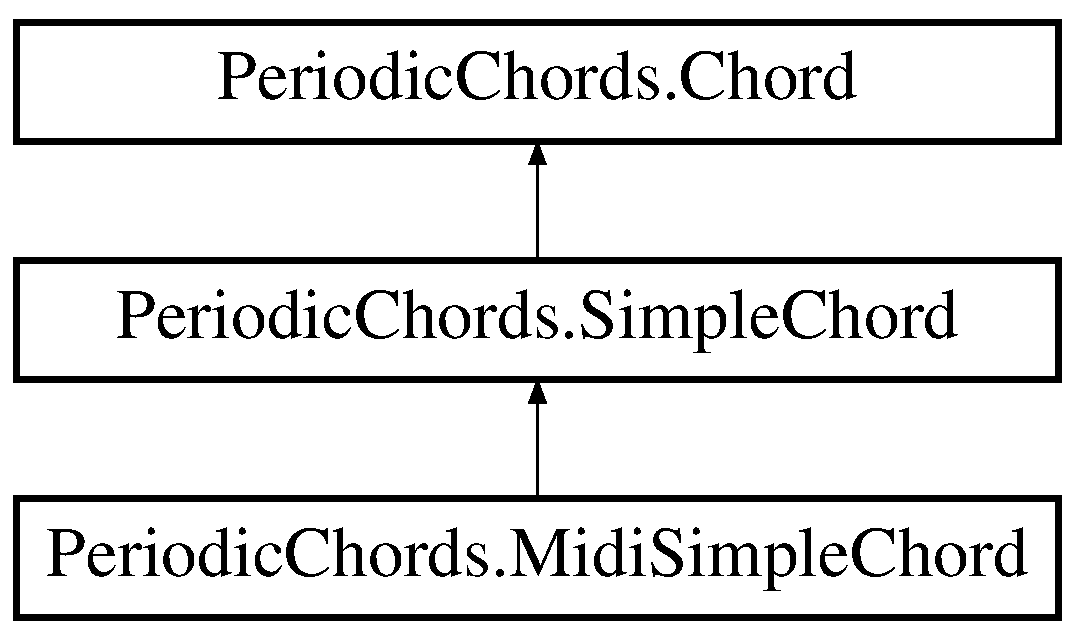
\includegraphics[height=3.000000cm]{class_periodic_chords_1_1_midi_simple_chord}
\end{center}
\end{figure}
\subsection*{Properties}
\begin{DoxyCompactItemize}
\item 
\hypertarget{class_periodic_chords_1_1_midi_simple_chord_ac60a8574539a8d9e909e26ace308e55f}{override double\mbox{[}$\,$\mbox{]} {\bfseries Frequencies}\hspace{0.3cm}{\ttfamily  \mbox{[}get\mbox{]}}}\label{class_periodic_chords_1_1_midi_simple_chord_ac60a8574539a8d9e909e26ace308e55f}

\item 
\hypertarget{class_periodic_chords_1_1_midi_simple_chord_a7f0bdddefff85af2f94de594ecacd9f8}{override double\mbox{[}$\,$\mbox{]} {\bfseries Notes}\hspace{0.3cm}{\ttfamily  \mbox{[}get\mbox{]}}}\label{class_periodic_chords_1_1_midi_simple_chord_a7f0bdddefff85af2f94de594ecacd9f8}

\end{DoxyCompactItemize}
\subsection*{Additional Inherited Members}


The documentation for this class was generated from the following file\+:\begin{DoxyCompactItemize}
\item 
C\+:/\+Users/praktykant/\+Documents/\+Git\+Hub/\+Harmony-\/\+Simulation/\+Harmony\+Editor/\+Periodic\+Chords/Simple\+Chord.\+cs\end{DoxyCompactItemize}

\hypertarget{class_populo_application_1_1_per_cent_numeric_up_down}{\section{Populo\+Application.\+Per\+Cent\+Numeric\+Up\+Down Class Reference}
\label{class_populo_application_1_1_per_cent_numeric_up_down}\index{Populo\+Application.\+Per\+Cent\+Numeric\+Up\+Down@{Populo\+Application.\+Per\+Cent\+Numeric\+Up\+Down}}
}


Defined Percent numericupdown control  


Inheritance diagram for Populo\+Application.\+Per\+Cent\+Numeric\+Up\+Down\+:\begin{figure}[H]
\begin{center}
\leavevmode
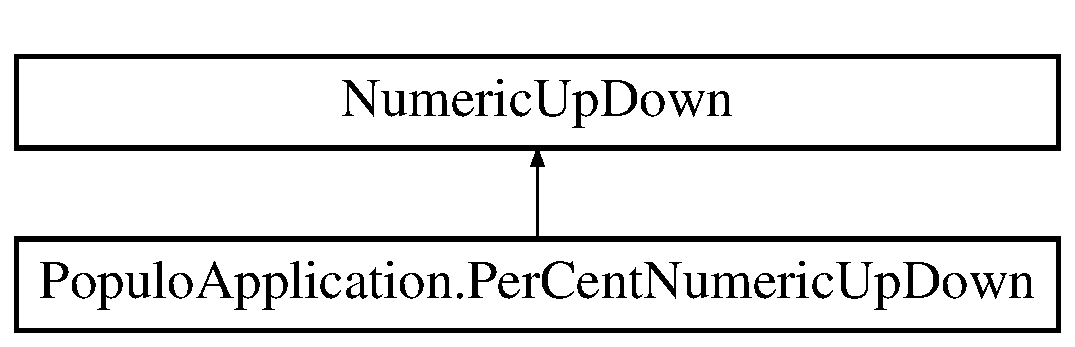
\includegraphics[height=2.000000cm]{class_populo_application_1_1_per_cent_numeric_up_down}
\end{center}
\end{figure}
\subsection*{Protected Member Functions}
\begin{DoxyCompactItemize}
\item 
\hypertarget{class_populo_application_1_1_per_cent_numeric_up_down_a11e3c2c4bab813f1d4f0dfd2b0314d6e}{override void {\bfseries Update\+Edit\+Text} ()}\label{class_populo_application_1_1_per_cent_numeric_up_down_a11e3c2c4bab813f1d4f0dfd2b0314d6e}

\end{DoxyCompactItemize}


\subsection{Detailed Description}
Defined Percent numericupdown control 



The documentation for this class was generated from the following file\+:\begin{DoxyCompactItemize}
\item 
C\+:/\+Users/praktykant/\+Documents/\+Git\+Hub/\+Harmony-\/\+Simulation/\+Populo/\+Populo\+Application/\+Windows/\+Controls/Per\+Cent\+Numeric\+Up\+Down.\+cs\end{DoxyCompactItemize}

\hypertarget{class_periodic_chords_1_1_period}{\section{Periodic\+Chords.\+Period Class Reference}
\label{class_periodic_chords_1_1_period}\index{Periodic\+Chords.\+Period@{Periodic\+Chords.\+Period}}
}
\subsection*{Public Member Functions}
\begin{DoxyCompactItemize}
\item 
\hypertarget{class_periodic_chords_1_1_period_a524d6b86e4fede75ce3840f79d59bd7f}{{\bfseries Period} (double period, uint repeats, double\mbox{[}$\,$\mbox{]} divides)}\label{class_periodic_chords_1_1_period_a524d6b86e4fede75ce3840f79d59bd7f}

\item 
\hypertarget{class_periodic_chords_1_1_period_a204b109c86b615911136b10e9a2605b5}{{\bfseries Period} (double period, uint repeats, double\mbox{[}$\,$\mbox{]} divides, uint number\+Of\+Divides)}\label{class_periodic_chords_1_1_period_a204b109c86b615911136b10e9a2605b5}

\item 
\hypertarget{class_periodic_chords_1_1_period_ab3bbccd315c5a88416bbf4831458df01}{double\mbox{[}$\,$\mbox{]} {\bfseries derivatives} (double base\+Value)}\label{class_periodic_chords_1_1_period_ab3bbccd315c5a88416bbf4831458df01}

\end{DoxyCompactItemize}
\subsection*{Properties}
\begin{DoxyCompactItemize}
\item 
\hypertarget{class_periodic_chords_1_1_period_a754288fdd271c484b18d4d27a4ca8884}{double {\bfseries Period\+A}\hspace{0.3cm}{\ttfamily  \mbox{[}get, set\mbox{]}}}\label{class_periodic_chords_1_1_period_a754288fdd271c484b18d4d27a4ca8884}

\item 
\hypertarget{class_periodic_chords_1_1_period_a0b93224ab6fc5af1b026dff27943ffa6}{uint {\bfseries Repeats}\hspace{0.3cm}{\ttfamily  \mbox{[}get, set\mbox{]}}}\label{class_periodic_chords_1_1_period_a0b93224ab6fc5af1b026dff27943ffa6}

\item 
\hypertarget{class_periodic_chords_1_1_period_aeb122e2539791f3dbdaa41fe1562bdd0}{double\mbox{[}$\,$\mbox{]} {\bfseries Divides}\hspace{0.3cm}{\ttfamily  \mbox{[}get, set\mbox{]}}}\label{class_periodic_chords_1_1_period_aeb122e2539791f3dbdaa41fe1562bdd0}

\end{DoxyCompactItemize}


The documentation for this class was generated from the following file\+:\begin{DoxyCompactItemize}
\item 
C\+:/\+Users/praktykant/\+Documents/\+Git\+Hub/\+Harmony-\/\+Simulation/\+Harmony\+Editor/\+Periodic\+Chords/Period.\+cs\end{DoxyCompactItemize}

\hypertarget{class_harmony_editor_1_1_period_editor}{\section{Harmony\+Editor.\+Period\+Editor Class Reference}
\label{class_harmony_editor_1_1_period_editor}\index{Harmony\+Editor.\+Period\+Editor@{Harmony\+Editor.\+Period\+Editor}}
}
Inheritance diagram for Harmony\+Editor.\+Period\+Editor\+:\begin{figure}[H]
\begin{center}
\leavevmode
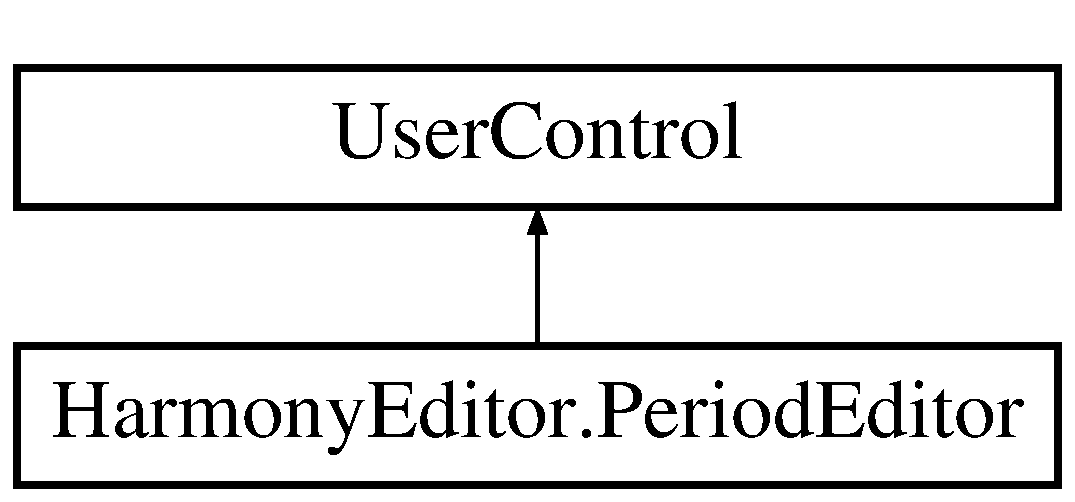
\includegraphics[height=2.000000cm]{class_harmony_editor_1_1_period_editor}
\end{center}
\end{figure}
\subsection*{Public Member Functions}
\begin{DoxyCompactItemize}
\item 
\hypertarget{class_harmony_editor_1_1_period_editor_a2a45b4f705ce8a28f7b990b92dcc5593}{void {\bfseries Clear} ()}\label{class_harmony_editor_1_1_period_editor_a2a45b4f705ce8a28f7b990b92dcc5593}

\end{DoxyCompactItemize}
\subsection*{Public Attributes}
\begin{DoxyCompactItemize}
\item 
\hypertarget{class_harmony_editor_1_1_period_editor_a901ae3e8aa448a3243c61c13df752a05}{Event\+Handler {\bfseries Was\+Validated}}\label{class_harmony_editor_1_1_period_editor_a901ae3e8aa448a3243c61c13df752a05}

\end{DoxyCompactItemize}
\subsection*{Protected Member Functions}
\begin{DoxyCompactItemize}
\item 
\hypertarget{class_harmony_editor_1_1_period_editor_a7bc3928e2a891722774568f4c1391ec6}{virtual void {\bfseries on\+Validation} ()}\label{class_harmony_editor_1_1_period_editor_a7bc3928e2a891722774568f4c1391ec6}

\item 
override void \hyperlink{class_harmony_editor_1_1_period_editor_a71c11fbb8292b277a56cccce4542d957}{Dispose} (bool disposing)
\begin{DoxyCompactList}\small\item\em Clean up any resources being used. \end{DoxyCompactList}\end{DoxyCompactItemize}
\subsection*{Properties}
\begin{DoxyCompactItemize}
\item 
\hypertarget{class_harmony_editor_1_1_period_editor_abe7f3f2e2f72b27ef60bb9b603df3285}{bool {\bfseries Valid}\hspace{0.3cm}{\ttfamily  \mbox{[}get\mbox{]}}}\label{class_harmony_editor_1_1_period_editor_abe7f3f2e2f72b27ef60bb9b603df3285}

\item 
\hypertarget{class_harmony_editor_1_1_period_editor_ae41df49a3acdf3040133f60552ab7ddb}{\hyperlink{class_periodic_chords_1_1_period}{Period} {\bfseries Value}\hspace{0.3cm}{\ttfamily  \mbox{[}get, set\mbox{]}}}\label{class_harmony_editor_1_1_period_editor_ae41df49a3acdf3040133f60552ab7ddb}

\item 
\hypertarget{class_harmony_editor_1_1_period_editor_a79a30bb78ce39cc4b22214ce40d95956}{bool {\bfseries Default}\hspace{0.3cm}{\ttfamily  \mbox{[}get\mbox{]}}}\label{class_harmony_editor_1_1_period_editor_a79a30bb78ce39cc4b22214ce40d95956}

\end{DoxyCompactItemize}


\subsection{Member Function Documentation}
\hypertarget{class_harmony_editor_1_1_period_editor_a71c11fbb8292b277a56cccce4542d957}{\index{Harmony\+Editor\+::\+Period\+Editor@{Harmony\+Editor\+::\+Period\+Editor}!Dispose@{Dispose}}
\index{Dispose@{Dispose}!Harmony\+Editor\+::\+Period\+Editor@{Harmony\+Editor\+::\+Period\+Editor}}
\subsubsection[{Dispose}]{\setlength{\rightskip}{0pt plus 5cm}override void Harmony\+Editor.\+Period\+Editor.\+Dispose (
\begin{DoxyParamCaption}
\item[{bool}]{disposing}
\end{DoxyParamCaption}
)\hspace{0.3cm}{\ttfamily [protected]}}}\label{class_harmony_editor_1_1_period_editor_a71c11fbb8292b277a56cccce4542d957}


Clean up any resources being used. 


\begin{DoxyParams}{Parameters}
{\em disposing} & true if managed resources should be disposed; otherwise, false.\\
\hline
\end{DoxyParams}


The documentation for this class was generated from the following files\+:\begin{DoxyCompactItemize}
\item 
C\+:/\+Users/praktykant/\+Documents/\+Git\+Hub/\+Harmony-\/\+Simulation/\+Harmony\+Editor/\+Harmony\+Editor/\+Controls/Period\+Editor.\+cs\item 
C\+:/\+Users/praktykant/\+Documents/\+Git\+Hub/\+Harmony-\/\+Simulation/\+Harmony\+Editor/\+Harmony\+Editor/\+Controls/Period\+Editor.\+Designer.\+cs\end{DoxyCompactItemize}

\hypertarget{class_periodic_chords_1_1_periodic_chord}{\section{Periodic\+Chords.\+Periodic\+Chord Class Reference}
\label{class_periodic_chords_1_1_periodic_chord}\index{Periodic\+Chords.\+Periodic\+Chord@{Periodic\+Chords.\+Periodic\+Chord}}
}
Inheritance diagram for Periodic\+Chords.\+Periodic\+Chord\+:\begin{figure}[H]
\begin{center}
\leavevmode
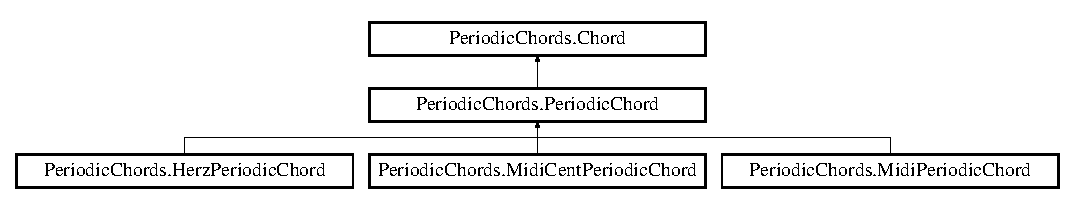
\includegraphics[height=2.295082cm]{class_periodic_chords_1_1_periodic_chord}
\end{center}
\end{figure}
\subsection*{Protected Member Functions}
\begin{DoxyCompactItemize}
\item 
\hypertarget{class_periodic_chords_1_1_periodic_chord_a6a0af17872bad7e2f59759b6f041dfe2}{override double\mbox{[}$\,$\mbox{]} {\bfseries get\+Values} ()}\label{class_periodic_chords_1_1_periodic_chord_a6a0af17872bad7e2f59759b6f041dfe2}

\end{DoxyCompactItemize}
\subsection*{Properties}
\begin{DoxyCompactItemize}
\item 
\hypertarget{class_periodic_chords_1_1_periodic_chord_aa3e10ced590f148788c4ba40878e35cc}{uint {\bfseries Base\+Note}\hspace{0.3cm}{\ttfamily  \mbox{[}get, set\mbox{]}}}\label{class_periodic_chords_1_1_periodic_chord_aa3e10ced590f148788c4ba40878e35cc}

\item 
\hypertarget{class_periodic_chords_1_1_periodic_chord_aaf74837a4f47ffe44b42d38071664c09}{\hyperlink{class_periodic_chords_1_1_period}{Period}\mbox{[}$\,$\mbox{]} {\bfseries Periods}\hspace{0.3cm}{\ttfamily  \mbox{[}get, set\mbox{]}}}\label{class_periodic_chords_1_1_periodic_chord_aaf74837a4f47ffe44b42d38071664c09}

\end{DoxyCompactItemize}
\subsection*{Additional Inherited Members}


The documentation for this class was generated from the following file\+:\begin{DoxyCompactItemize}
\item 
C\+:/\+Users/praktykant/\+Documents/\+Git\+Hub/\+Harmony-\/\+Simulation/\+Harmony\+Editor/\+Periodic\+Chords/Periodic\+Chord.\+cs\end{DoxyCompactItemize}

\hypertarget{class_periodic_chords_1_1_pitch_data}{\section{Periodic\+Chords.\+Pitch\+Data Class Reference}
\label{class_periodic_chords_1_1_pitch_data}\index{Periodic\+Chords.\+Pitch\+Data@{Periodic\+Chords.\+Pitch\+Data}}
}
\subsection*{Properties}
\begin{DoxyCompactItemize}
\item 
\hypertarget{class_periodic_chords_1_1_pitch_data_abe473d97cf439c72fd7a40198f6f01b4}{double\mbox{[}$\,$\mbox{]} {\bfseries Pitches}\hspace{0.3cm}{\ttfamily  \mbox{[}get, set\mbox{]}}}\label{class_periodic_chords_1_1_pitch_data_abe473d97cf439c72fd7a40198f6f01b4}

\item 
\hypertarget{class_periodic_chords_1_1_pitch_data_aaaa5e93ce6101b04692c64359396cbe3}{int {\bfseries Left}\hspace{0.3cm}{\ttfamily  \mbox{[}get, set\mbox{]}}}\label{class_periodic_chords_1_1_pitch_data_aaaa5e93ce6101b04692c64359396cbe3}

\item 
\hypertarget{class_periodic_chords_1_1_pitch_data_afc7f131d95a1eda021ebb3a562782f4c}{int {\bfseries Right}\hspace{0.3cm}{\ttfamily  \mbox{[}get, set\mbox{]}}}\label{class_periodic_chords_1_1_pitch_data_afc7f131d95a1eda021ebb3a562782f4c}

\end{DoxyCompactItemize}


The documentation for this class was generated from the following file\+:\begin{DoxyCompactItemize}
\item 
C\+:/\+Users/praktykant/\+Documents/\+Git\+Hub/\+Harmony-\/\+Simulation/\+Harmony\+Editor/\+Periodic\+Chords/\+Serialization/Pitch\+Data.\+cs\end{DoxyCompactItemize}

\hypertarget{classpopulo_1_1_program}{\section{populo.\+Program Class Reference}
\label{classpopulo_1_1_program}\index{populo.\+Program@{populo.\+Program}}
}
\subsection*{Static Public Member Functions}
\begin{DoxyCompactItemize}
\item 
\hypertarget{classpopulo_1_1_program_a3e97a9050cf639b4eb65a13d17b7913f}{static void {\bfseries Main} (string\mbox{[}$\,$\mbox{]} args)}\label{classpopulo_1_1_program_a3e97a9050cf639b4eb65a13d17b7913f}

\end{DoxyCompactItemize}


The documentation for this class was generated from the following file\+:\begin{DoxyCompactItemize}
\item 
C\+:/\+Users/praktykant/\+Documents/\+Git\+Hub/\+Harmony-\/\+Simulation/\+Populo/\+Test\+Populo/Program.\+cs\end{DoxyCompactItemize}

\hypertarget{class_periodic_chords_1_1_simple_chord}{\section{Periodic\+Chords.\+Simple\+Chord Class Reference}
\label{class_periodic_chords_1_1_simple_chord}\index{Periodic\+Chords.\+Simple\+Chord@{Periodic\+Chords.\+Simple\+Chord}}
}
Inheritance diagram for Periodic\+Chords.\+Simple\+Chord\+:\begin{figure}[H]
\begin{center}
\leavevmode
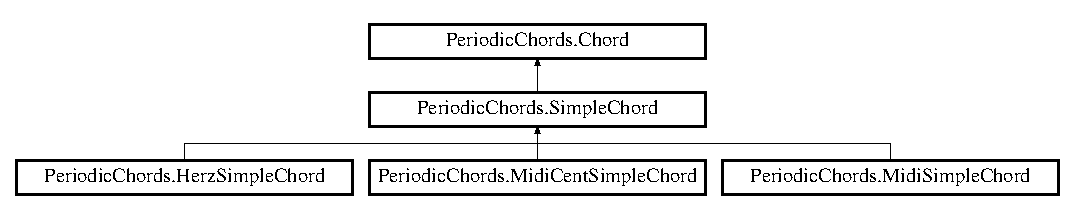
\includegraphics[height=2.393162cm]{class_periodic_chords_1_1_simple_chord}
\end{center}
\end{figure}
\subsection*{Protected Member Functions}
\begin{DoxyCompactItemize}
\item 
\hypertarget{class_periodic_chords_1_1_simple_chord_ad4bd98831bf186378108e76d34227f13}{override double\mbox{[}$\,$\mbox{]} {\bfseries get\+Values} ()}\label{class_periodic_chords_1_1_simple_chord_ad4bd98831bf186378108e76d34227f13}

\end{DoxyCompactItemize}
\subsection*{Properties}
\begin{DoxyCompactItemize}
\item 
\hypertarget{class_periodic_chords_1_1_simple_chord_a3cbf7fcba934e14e05106f6b6c511c30}{double\mbox{[}$\,$\mbox{]} {\bfseries Peaks}\hspace{0.3cm}{\ttfamily  \mbox{[}get, set\mbox{]}}}\label{class_periodic_chords_1_1_simple_chord_a3cbf7fcba934e14e05106f6b6c511c30}

\end{DoxyCompactItemize}
\subsection*{Additional Inherited Members}


The documentation for this class was generated from the following file\+:\begin{DoxyCompactItemize}
\item 
C\+:/\+Users/praktykant/\+Documents/\+Git\+Hub/\+Harmony-\/\+Simulation/\+Harmony\+Editor/\+Periodic\+Chords/Simple\+Chord.\+cs\end{DoxyCompactItemize}

\hypertarget{class_harmony_editor_1_1_simple_chord_editor}{\section{Harmony\+Editor.\+Simple\+Chord\+Editor Class Reference}
\label{class_harmony_editor_1_1_simple_chord_editor}\index{Harmony\+Editor.\+Simple\+Chord\+Editor@{Harmony\+Editor.\+Simple\+Chord\+Editor}}
}
Inheritance diagram for Harmony\+Editor.\+Simple\+Chord\+Editor\+:\begin{figure}[H]
\begin{center}
\leavevmode
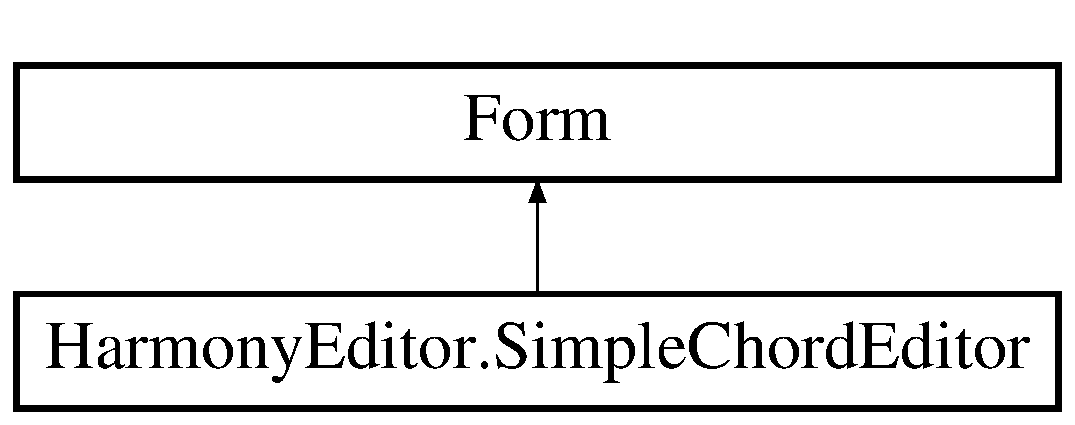
\includegraphics[height=2.000000cm]{class_harmony_editor_1_1_simple_chord_editor}
\end{center}
\end{figure}
\subsection*{Public Member Functions}
\begin{DoxyCompactItemize}
\item 
\hypertarget{class_harmony_editor_1_1_simple_chord_editor_a0f53a8a071c6351dfbee7a5806d49753}{{\bfseries Simple\+Chord\+Editor} (\hyperlink{class_periodic_chords_1_1_simple_chord}{Simple\+Chord} chord)}\label{class_harmony_editor_1_1_simple_chord_editor_a0f53a8a071c6351dfbee7a5806d49753}

\end{DoxyCompactItemize}
\subsection*{Protected Member Functions}
\begin{DoxyCompactItemize}
\item 
override void \hyperlink{class_harmony_editor_1_1_simple_chord_editor_a9293aff01254ab51d2765bcfebe28d53}{Dispose} (bool disposing)
\begin{DoxyCompactList}\small\item\em Clean up any resources being used. \end{DoxyCompactList}\end{DoxyCompactItemize}
\subsection*{Properties}
\begin{DoxyCompactItemize}
\item 
\hypertarget{class_harmony_editor_1_1_simple_chord_editor_a484b8e9a4e6f485f5c58df6da7811b3d}{\hyperlink{class_periodic_chords_1_1_simple_chord}{Simple\+Chord} {\bfseries Result}\hspace{0.3cm}{\ttfamily  \mbox{[}get\mbox{]}}}\label{class_harmony_editor_1_1_simple_chord_editor_a484b8e9a4e6f485f5c58df6da7811b3d}

\item 
\hypertarget{class_harmony_editor_1_1_simple_chord_editor_aad6159339b4e9010aae29b664ae644e3}{bool {\bfseries Ok\+Clicked}\hspace{0.3cm}{\ttfamily  \mbox{[}get\mbox{]}}}\label{class_harmony_editor_1_1_simple_chord_editor_aad6159339b4e9010aae29b664ae644e3}

\end{DoxyCompactItemize}


\subsection{Member Function Documentation}
\hypertarget{class_harmony_editor_1_1_simple_chord_editor_a9293aff01254ab51d2765bcfebe28d53}{\index{Harmony\+Editor\+::\+Simple\+Chord\+Editor@{Harmony\+Editor\+::\+Simple\+Chord\+Editor}!Dispose@{Dispose}}
\index{Dispose@{Dispose}!Harmony\+Editor\+::\+Simple\+Chord\+Editor@{Harmony\+Editor\+::\+Simple\+Chord\+Editor}}
\subsubsection[{Dispose}]{\setlength{\rightskip}{0pt plus 5cm}override void Harmony\+Editor.\+Simple\+Chord\+Editor.\+Dispose (
\begin{DoxyParamCaption}
\item[{bool}]{disposing}
\end{DoxyParamCaption}
)\hspace{0.3cm}{\ttfamily [protected]}}}\label{class_harmony_editor_1_1_simple_chord_editor_a9293aff01254ab51d2765bcfebe28d53}


Clean up any resources being used. 


\begin{DoxyParams}{Parameters}
{\em disposing} & true if managed resources should be disposed; otherwise, false.\\
\hline
\end{DoxyParams}


The documentation for this class was generated from the following files\+:\begin{DoxyCompactItemize}
\item 
C\+:/\+Users/praktykant/\+Documents/\+Git\+Hub/\+Harmony-\/\+Simulation/\+Harmony\+Editor/\+Harmony\+Editor/\+Windows/Simple\+Chord\+Editor.\+cs\item 
C\+:/\+Users/praktykant/\+Documents/\+Git\+Hub/\+Harmony-\/\+Simulation/\+Harmony\+Editor/\+Harmony\+Editor/\+Windows/Simple\+Chord\+Editor.\+Designer.\+cs\end{DoxyCompactItemize}

\hypertarget{class_periodic_chords_1_1_sound_out_of_range_exception}{\section{Periodic\+Chords.\+Sound\+Out\+Of\+Range\+Exception Class Reference}
\label{class_periodic_chords_1_1_sound_out_of_range_exception}\index{Periodic\+Chords.\+Sound\+Out\+Of\+Range\+Exception@{Periodic\+Chords.\+Sound\+Out\+Of\+Range\+Exception}}
}
Inheritance diagram for Periodic\+Chords.\+Sound\+Out\+Of\+Range\+Exception\+:\begin{figure}[H]
\begin{center}
\leavevmode
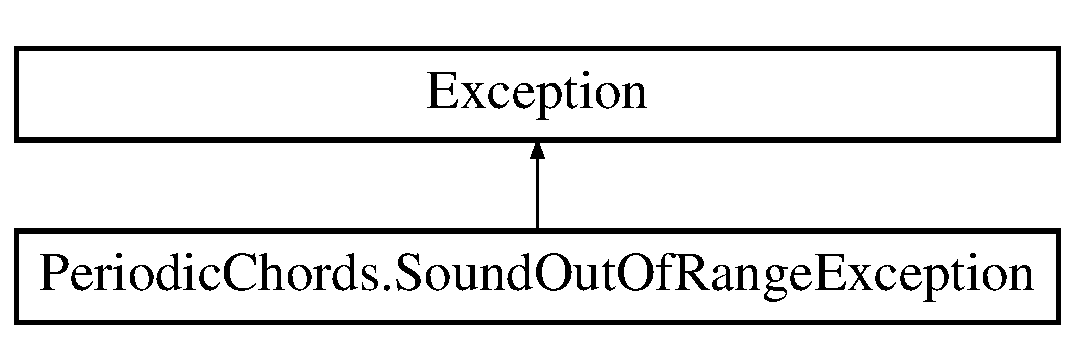
\includegraphics[height=2.000000cm]{class_periodic_chords_1_1_sound_out_of_range_exception}
\end{center}
\end{figure}
\subsection*{Public Member Functions}
\begin{DoxyCompactItemize}
\item 
\hypertarget{class_periodic_chords_1_1_sound_out_of_range_exception_abd13be5d6f01f29a1a01a0622efd915b}{{\bfseries Sound\+Out\+Of\+Range\+Exception} (string message)}\label{class_periodic_chords_1_1_sound_out_of_range_exception_abd13be5d6f01f29a1a01a0622efd915b}

\item 
\hypertarget{class_periodic_chords_1_1_sound_out_of_range_exception_ac86e331d7e21c689f5bf087b61e67aaf}{{\bfseries Sound\+Out\+Of\+Range\+Exception} (string message, Exception inner)}\label{class_periodic_chords_1_1_sound_out_of_range_exception_ac86e331d7e21c689f5bf087b61e67aaf}

\end{DoxyCompactItemize}


The documentation for this class was generated from the following file\+:\begin{DoxyCompactItemize}
\item 
C\+:/\+Users/praktykant/\+Documents/\+Git\+Hub/\+Harmony-\/\+Simulation/\+Harmony\+Editor/\+Periodic\+Chords/Exceptions.\+cs\end{DoxyCompactItemize}

\hypertarget{class_harmony_editor_1_1_spectrum}{\section{Harmony\+Editor.\+Spectrum Class Reference}
\label{class_harmony_editor_1_1_spectrum}\index{Harmony\+Editor.\+Spectrum@{Harmony\+Editor.\+Spectrum}}
}
Inheritance diagram for Harmony\+Editor.\+Spectrum\+:\begin{figure}[H]
\begin{center}
\leavevmode
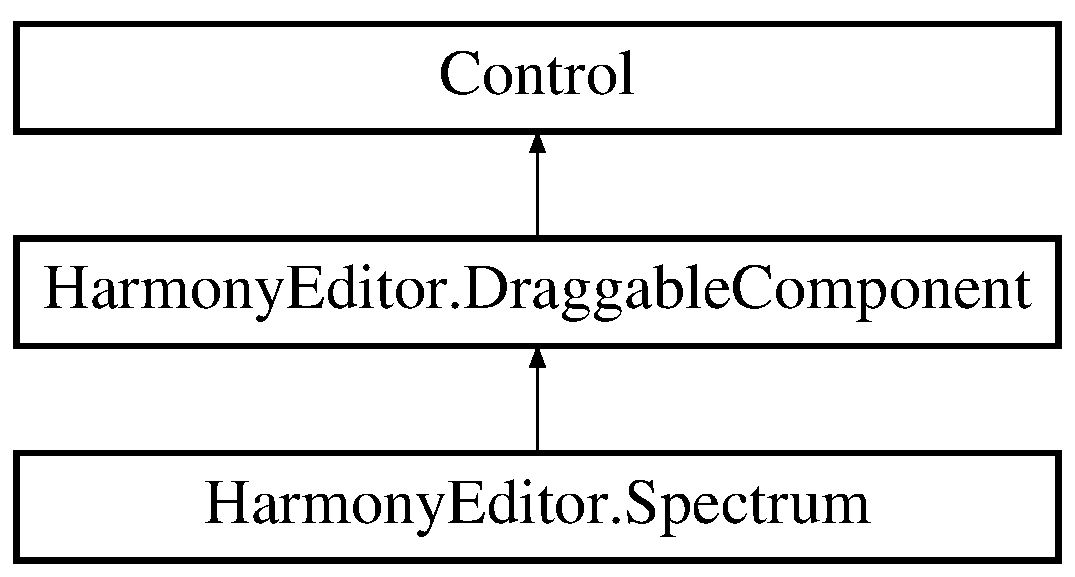
\includegraphics[height=3.000000cm]{class_harmony_editor_1_1_spectrum}
\end{center}
\end{figure}
\subsection*{Public Member Functions}
\begin{DoxyCompactItemize}
\item 
\hypertarget{class_harmony_editor_1_1_spectrum_a26ee8eba598ed569eb1e363b6676328c}{{\bfseries Spectrum} (bool rotated, bool freqnotes, \hyperlink{class_periodic_chords_1_1_chord}{Chord} chord, int width, int height)}\label{class_harmony_editor_1_1_spectrum_a26ee8eba598ed569eb1e363b6676328c}

\end{DoxyCompactItemize}
\subsection*{Protected Member Functions}
\begin{DoxyCompactItemize}
\item 
\hypertarget{class_harmony_editor_1_1_spectrum_aa6e1f0f21ee8671f5f32e785b7b4d076}{override void {\bfseries On\+Paint} (Paint\+Event\+Args pe)}\label{class_harmony_editor_1_1_spectrum_aa6e1f0f21ee8671f5f32e785b7b4d076}

\end{DoxyCompactItemize}
\subsection*{Properties}
\begin{DoxyCompactItemize}
\item 
\hypertarget{class_harmony_editor_1_1_spectrum_a993abb04ea909dbebad7da17e10cc642}{\hyperlink{class_periodic_chords_1_1_chord}{Chord} {\bfseries Cur\+Chord}\hspace{0.3cm}{\ttfamily  \mbox{[}get, set\mbox{]}}}\label{class_harmony_editor_1_1_spectrum_a993abb04ea909dbebad7da17e10cc642}

\item 
\hypertarget{class_harmony_editor_1_1_spectrum_ad57883de83d316e57be550b6f883d000}{bool {\bfseries Rotated}\hspace{0.3cm}{\ttfamily  \mbox{[}get, set\mbox{]}}}\label{class_harmony_editor_1_1_spectrum_ad57883de83d316e57be550b6f883d000}

\item 
\hypertarget{class_harmony_editor_1_1_spectrum_a72c7c1f115b7b903f874066fe9610439}{bool {\bfseries Freq\+Notes}\hspace{0.3cm}{\ttfamily  \mbox{[}get, set\mbox{]}}}\label{class_harmony_editor_1_1_spectrum_a72c7c1f115b7b903f874066fe9610439}

\end{DoxyCompactItemize}
\subsection*{Additional Inherited Members}


The documentation for this class was generated from the following file\+:\begin{DoxyCompactItemize}
\item 
C\+:/\+Users/praktykant/\+Documents/\+Git\+Hub/\+Harmony-\/\+Simulation/\+Harmony\+Editor/\+Harmony\+Editor/\+Controls/Spectrum.\+cs\end{DoxyCompactItemize}

%--- End generated contents ---

% Index
\newpage
\phantomsection
\addcontentsline{toc}{chapter}{Index}
\printindex

\end{document}
